\documentclass{thesis}

\usepackage{amsthm}
\usepackage{charter}
\usepackage{eulervm}
\usepackage{amsmath}
\usepackage{amssymb}
\usepackage{graphicx}
\usepackage{caption}
\usepackage{subcaption}
\usepackage{enumerate}
\usepackage{cancel}
\usepackage{hyperref}
\usepackage{makeidx}
\usepackage{footmisc}
\usepackage{mathrsfs}
\usepackage{float}

\theoremstyle{definition}
\newtheorem{theorem}{Theorem}
\newtheorem{definition}{Definition}
\newtheorem{corollary}{Corollary}
\newtheorem{lemma}{Lemma}
\newtheorem{example}{Example}
\setcounter{tocdepth}{4}
\floatstyle{ruled}
\newfloat{pseudo}{h}{lop}
\floatname{pseudo}{Algorithm}

%\let\doendproof\endproof
%\renewcommand\endproof{~\hfill\qed\doendproof}

\usepackage{color}
\usepackage[usenames,dvipsnames,svgnames,table]{xcolor}

\newcommand{\argmin}{\mathop{\arg\min}}
%\DeclareMathOperator*{\argmin}{\arg\,\min}
\DeclareMathOperator*{\argmax}{\arg\,\max}
\DeclareMathOperator*{\nid}{NID}
\DeclareMathOperator*{\id}{ID}

\newcommand{\sdr}[1]{\textcolor{blue}{\small #1\textsuperscript{[sdr]} }}
\newcommand{\pb}[1]{\textcolor{OliveGreen}{\small #1 \textsuperscript{[pb]} }}

\newcommand{\p}{\,\text{.}}
\newcommand{\fl}[1]{\left \lfloor #1 \right \rfloor}
\newcommand{\g}[1]{\color{gray} #1 \color{black}}
\newcommand{\B}{{\mathbb B}}
\newcommand{\R}{{\mathbb R}}
\newcommand{\N}{{\mathbb N}}
\newcommand{\C}{{\cal C}}
\newcommand{\M}{{\cal M}}
\newcommand{\T}{{\cal T}}
\newcommand{\F}{{\cal F}}
\renewcommand{\P}{\mathscr P}
\newcommand{\K}{{\cal K}}
\newcommand{\X}{{\cal X}}
\newcommand{\D}{\Delta}
\newcommand{\Nm}{{\cal N}}
\newcommand{\m}{{\overline{m}}}
\newcommand{\ok}{{\overline{\kappa}}}
\newcommand{\mmid}{\;\middle|\;}
\newcommand{\tn}[1]{\textnormal{#1}}
\newcommand{\pair}[1]{\left\langle{#1}\right\rangle}
\newcommand{\tuple}[1]{\left\langle{#1}\right\rangle}
\newcommand{\concat}{\oplus}
\newcommand{\symb}[1]{\texttt{#1}}
\newcommand{\br}[1]{\overline{#1}}
\newcommand{\s}{S}
\newcommand{\bi}{\bar\imath}
\newcommand{\dom}[1]{\mathop{\tn{dom}(#1)}}
\newcommand{\range}[1]{\mathop{\tn{range}(#1)}}
\newcommand{\Cc}{C_\tn{comp}}
\newcommand{\G}{{\mathbb G}}
\newcommand{\cG}{{\mathcal G}}
\newcommand{\tab}{\hspace*{5mm}}
\newcommand{\bD}{\boldsymbol\Lambda}
\newcommand{\bm}{\boldsymbol\mu}
\newcommand{\cN}{{\cal N}}
\newcommand{\bs}[1]{{\boldsymbol {#1} }}
\newcommand{\hide}[1]{}
\newcommand{\ol}[1]{\overline{#1}}

\setcounter{tocdepth}{1}

\title{The single sample setting \\ \normalsize \emph{Exercises in learning from just one example}}
\date{\today}

% non-indented, spaced paragraphs
\setlength{\parindent}{0.0in}
\setlength{\parskip}{0.1in}

\makeindex

\begin{document}

\maketitle

\tableofcontents

\chapter*{Summary}
\noindent What can be learned from a single example? If we are faced with some complex process, producing large intricate constructs, but we are only given one example of its output, can we still draw conclusions about the source, or ascribe meaning to the patterns we find? This is by no means just an academic exercise: we only have one Internet, for example, only one climate system and only one global financial system. What assumptions must we make about the processes that generated them, in order to learn about their structure? What can we do if we make no assumptions at all? Each chapter of this dissertation studies a perspective on this question, starting with a high-level theoretical approach, and gradually working towards more practical aspects.
 
The first chapter provides an informal introduction to this question, and the tools we use to study it. In \textbf{Chapter~\ref{chapter:safe}}, we view the problem in its most general form, using the principle of \emph{Kolmogorov complexity}. Kolmogorov complexity makes only one assumption: that the source of the data can be understood as a computational process. Under this assumption, it gives us an objective definition of the data's \emph{information content}. As is well known, the incomputable Kolmogorov complexity can be bounded from above by computable means. We show that with additional assumptions about the source of the data, such as its computational complexity, we can compute a value that is not just an upper bound, but also, with high probability, a good approximation. We also analyze functions derived from Kolmogorov complexity, such as the \emph{normalized information distance}: we show that good approximations to Kolmogorov complexity do not necessarily translate to good approximations of derived functions, but with careful analysis, we can provide some guarantees.

\textbf{Chapter\ref{chapter:problem}} deals with model selection. Given only a single sample, what can we say about the complexity of its source? How much of the data is structure, and how much is random? This question has been studied under many names, like \emph{sophistication}, the \emph{algorithmic sufficient statistic} and  \emph{effective complexity}. We show that all these approaches have fundamental problems: the functions proposed \emph{cannot} correspond to the intuition that inspired them. It remains an open question whether objective model selection in this setting is possible, but we provide several arguments that suggest the answer is negative.

In \textbf{Chapter~\ref{chapter:fractals}} we turn to a practical application of the single sample setting: large complex graphs. These are complex objects, with rich internal structure, but no straightforward way to divide the data into chunks with similar properties. One solution is to find small, frequently recurring subgraphs, known as \emph{network motifs}. However, the fact that a subgraph is frequent is by itself no indication that it is a meaningful pattern: many subgraphs occur frequently, simply by chance. To show that a particular subgraph is special, we must show that its occurrences are \emph{unexpected} for a particular source. Using the Minimum Description Length principle, the practical cousin of Kolmogorov complexity, we develop a fast way to judge whether such subgraphs are unexpected. This allows motif analysis to scale to much larger graphs than was possible with traditional techniques.

Where the previous chapter studies the recurrence of similar structures at the same scale, \textbf{Chapter~\ref{chapter:fractals}} investigates \emph{self-similarity}: the recurrence of the same structure across scales. This is often a crucial assumption in graph analysis: we cannot analyse the whole of the World Wide Web, so we assume that a large subgraph, extracted from a random walk, has the same properties as the whole. Learning self-similar structure is known as the \emph{fractal inverse problem}, a long-standing open question. We analyze the fractal inverse problem in the domain of point patterns in Euclidean spaces, and show that it can be solved using an EM algorithm. 

The field of statistics is divided neatly by the type of data under analysis. The available models and techniques differ sharply from times series to sets of iid. samples, to geospatial information. The single sample setting provides us with a general perspective: it shows that in all cases we are dealing with a single, finite example from some partially random, computable source. The type of the data is simply an assumption we make about its source, usually to let us divide the data in chunks, so that the similarities and differences between these chunks will let us reconstruct the source from the data. This view is instructive when we are faced with modern types of data like complex graphs, where the question of how to subdivide the data is not easily answered. The perspective of single sample statistics gives us a starting point: we can always consider the data a single sample from some computable distribution.

\chapter{Introduction}
\label{chapter:introduction}
\begin{quote}
He waved a photograph of the Phaistos Disc. `The people who made this. Four thousand years ago! They used stamps! And if they were such pre-alfabetic genuises, then surely this must say something interesting, mustn't it? So I should be the first to read it, shouldn't I? The miserable thing is we have only this one specimen. But you don't make stamps for just one tablet, do you?'[\ldots]

`Let me explain my predicament to you.' He picked a newspaper up from the floor, and scribbled something in the margins.
`Write down the following number: eighty-three billion one hundred and ninety-one million twenty-four thousand five hundred and sixty-seven.' And after she had written it down on the sheet she used for her notes: `Now imagine an aboriginal cryptographer in an ancient Australian forest, who doesn't even know that those are numbers; all he sees is eleven incomprehensible marks: 8 3 1 9 1 0 2 4 5 6 7. They're all different, except the repeated symbol 1. Wat can he conclude from this? Nothing at all. That's the point I'm at now. Imagine that he suddenly has the brilliant idea that they're numbers, how is he supposed to figure out that they're alphabetically ordered, Dutch numerals from one to ten? How is he supposed to figure out that ``acht'' is the name of the number 8? He doesn't even know the decimal system, let alone the Dutch language.\\
---\emph{The Discovery of Heaven}, Harry Mulish \cite{mulisch1996discovery} 
\end{quote}

In the early chapters of the novel \emph{The Discovery of Heaven} we meet Onno Quist: a disorganized, left-wing philologist, who has become obsessed with a mysterious artifact discovered centuries ago in the ruins of the Minoan palace on Crete, the \emph{Phaistos disc}. The disc actually exists. It contains a spiralling sequence of 242 symbols, from an alphabet of 45 distinct signs. Quist is convinced the disc holds an important message, and is sufficiently lacking in humility to decide that he must be the one to decipher it. But the strange marking that adorn the Phaistos disc are not found anywhere else. The disc is the only example of this kind of writing.

\index{The Discovery of Heaven} \index{Harry Mulisch} \index{Phaistos Disc}

Quist is living a scientist's nightmare. Not for nothing are studies with small sample sizes easily dismissed as near-meaningless. To make strong inferences and hard claims, we cannot do without many repetitions: large amounts of examples of the same type of thing, over and over again. The recent announcement of the discovery of the Higgs Boson, inferred from experimental data with the famously stringent $5\sigma$ level of statistical significance that particle physics requires, took 300 trillion repetitions of the proton collision experiment that the Large Hadron Collider was built for. For a particle physicist, attempting anything with just one sample, must feel like digging a railway tunnel with a toothpick.

\index{Higgs Boson} \index{$5\sigma$} \index{Large Hadron Collider}

There is still, however, considerable difference between one sample and no samples at all. Consider this classic scenario, used the world over to instruct students in the basics of statistics: a soldier for a nation engaged in a bitter ground war is debriefed after being rescued from behind enemy lines. He relates to his superiors that he witnessed a new type of tank in a training exercise. The tank is clearly a secret weapon, and far in advance of anything their side can produce. The officers become anxious and wish to know how many of these tanks the enemy posess. The soldier only saw one, but he can relate that its serial number was 17.

\index{German tank problem}

Assuming that the enemy number their tanks in sequence, and that the soldier was as likely to spot this tank as any other, what does this one observation tell us about the number of tanks produced? Clearly, there are at least 17, but how many beyond that? What would be a good guess? One approach would be to take the number of tanks $n$ for which this outcome (a soldier spotting tank number 17) is most likely. For $n$ less than 17, seeing tank 17 is impossible, and for higher $n$ the probability of observing any particular tank is $1/n$. Thus, by this criterion we will guess that the enemy made just 17 tanks, and our soldier just happened to stumble on the one with the highest serial number. This seems like an optimistic conclusion, so perhaps we need to adjust our criterion.

Instead of choosing the $n$ for which our particular outcome is the most likely, let us try to find a different procedure; one that (a) ensures that the average of many repeats of this experiment (one soldier, one tank) converges to the true value, and (b) produces the smallest expected difference between our guess and the true value. Such a procedure is known as an \emph{unbiased minimum-variance estimator}. For this problem, one exists, and it tells us to expect that the enemy has 33 tanks. It also tells us that if we want to make a statement with 95\% confidence, we should say that the enemy has between 16 and 341 tanks. Still a great deal of uncertainty, but much better than we would have had if we had dismissed the single sample as useless. This is not just an exercise to stimulate the minds of young students. During the second world war, the Allies used exactly this procedure to estimate the number of Mark V tanks the Germans were producing (although they had more than one observation to work with) \cite{davies2006statistical}.

This type of trick is not much help to Onno Quist. The Phaistos disc contains no serial number, or at least not one that we can read. And if it did, estimating the production capability of the ancient Minoans is of no more help in {translating} the contents of the disc, than the tank's serial number would be in guessing the names of its occupants. But Onno does have one advantage that the beleaguered nation didn't have: the Phaistos disc contains \emph{internal structure}. We can count its symbols, look at their frequencies, their proximities and co-occurrences. The single number 17 could not be cracked open in this way to to find more information.

And in this respect Onno is not so lonely in his quest. While few scientists are asked to use just one sample to estimate the mean life expectancy, or the median income of a population, when the objects under study become more complex and richly structured, the number of examples available usually drops. Take the current webgraph, for example: the densely connected web of links between webpages on the internet. This is one of the most important ``objects'' of study in the world today. Unlocking just part of its structure catapulted Google into the company it is today. And like Onno, students of the web graph have only one example to work with. Climate researchers may sympathise. Until our telescopes improves their resolution, we have only one liquid-water planet whose atmosphere we can investigate. Speaking of telescopes, until 2003, astronomers had no proof that other stars even \emph{had} planets circling them, and the only sample of a solar system they had access to was our own. 

\index{web graph} \index{Google} \index{Solar system}

So what can be done? How far can Quist hope to get with the Phaistos disc? The world of statistics, machine learning and data mining offers a vast landscape of approaches. A landscape, that is, unfortunately, rather chaotic. The statisticians are divided in two camps, Frequentists and Bayesians, with incompatible ideas of what constitutes a probability. Furthermore, there is a zoo of different types of data: 
independent draws, or draws arranged in time, both in single dimensions or multiple, each draw may be from a fixed, finite number of outcomes, or from a continuous spectrum. And then there are objects like networks and trees, rich in structure, but requiring a whole new approach.

How can we capture this entire landscape in a single framework? Imagine a large room, filled with a vast number of machines. The machines are started, and each begins to write a sequence of ones and zeroes to a tape. Some machines will run indefinitely, and some, after a while, will stop. Each machine operates like clockwork: once started it will follow the exact same sequence of steps every time. The only thing that affects this deterministic operation is the ability the machines have to ask for randomness. The machine, at any point, can ask for a random input. If it does, the operation of the machine pauses, we flip a coin, and provide the machine with the result: 1 if the coin lands head and 0 if it lands tails. Since we don't feel like standing around waiting for the machines to ask us for coinflips, we simply flip a large number of coins in advance, write the results on a large tape, and let the machine read from this tape as it pleases.

Now imagine that we are given a finite sequence of ones and zeroes, a \emph{bitstring}, and we are told only that it came from one of the machines. The question put to us, is which machine produced the data? This is a metaphor for the business of inference. The world is a collection of processes. Each partly deterministic, and partly random. Our data is some set of observations from one of these processes: perhaps a human brain formulating an order for movie tickets, perhaps a human investigator sampling the heights of randomly selected individuals. You may object that none of these datasets are bitstrings, but they can all be encoded as such. In fact any statistician using a computer to analyze her data must admit that whatever shape or properties she assumes her data has, the way it is stored on the harddrive of her laptop is as a string of ones and zeroes.

But of course, we haven't described what these machines are. How should we build them? By what rules do they operate? Can we define a family of machines so that any process that might produce our data is equivalent to some machine in our family? It turns out that there is such a family, called Turing machines. These are purely mathematical constructs, and although occasionally a computer scientist with time to spare will build one out of Meccano or Lego, they are mostly studied with pen and paper. As we will see in the next chapter, there are very good reasons to believe that any process we can hope to understand is equivalent to a Turing machine. We can't say that the family of Turing machines captures all the processes that we may encounter in the universe, but they certainly seem to capture all the ones that we can understand.

This will be our framework. We have encountered some data, and we will assume that a Turing machine (or some process equivalent to it) has produced it. If we assume that we have unlimited resources at our disposal, what can we hope to do? We could test every machine: try every sequence of coinflips as input. Many machines are capable of producing our data, but for which machines is it most likely that they produced our data? This is a simple matter: for every sequence of random bits for which the machine produces our data, the probability is $\frac{1}{2} \times \frac{1}{2} \times \frac{1}{2}\times \ldots$ and so on, for as many bits as we fed the machine. That is, if we fed the machine $n$ bits, the probability of the machine producing our data in this way is $2^{-n}$. If there are multiple sequences for which the machine produces our data, we can sum their probabilities. We will introduce some notation to represent these ideas concisely: let $T$ represent one of the machines, and let $y$ be a sequence of bits that we should feed the machine so that it produces our data $x$. We then write:
\[
T(y) = x \p
\]

Unfortunately, there is always a machine that doesn't require any random bits, and simply produces our data whenever we start it. For any dataset, such a machine exists, encoding the data in the details of its cogs and wheels. For this machine, the probability of seeing our data is 1. By our current logic, this is always the best explanation for our data. But this isn't very satisfying. If Onno Quist translated the Phaistos Disc to a bitstring and found such a machine, he would not be very satisfied. Somehow, we need to penalize machines that encode to much of the data in their internals. The solution is found in \emph{universal} machines. Somewhere in our vast room of infinite machines, there are machines that work as follows: they first choose, using the coinflips, a random other machine, in such a way that any machine can be chosen, and then proceed to \emph{simulate} that machine.

Instead of asking which of the many machines produced our data, we can simply assume that the universal machine produced it, and ask which is the shortest sequence of random coinflips that causes the universal machine to produce our data. This sequence encodes first a machine, and then a sequence of random bits to feed to that machine to get our data. This simple idea has two very important consequences. Consequences that have allowed theoretical computer scientists to build a theory that connects statistics, computer science and philosophy: the theory of Kolmogorov complexity.

The first consequence is the connection between a \emph{description} of our data, and its \emph{probability}. If we take the sequence of random bits that causes our universal machine to produce our data, we can send it to somebody else, somebody who knows which universal machine we've chosen, and they can reconstruct the data from just this sequence. Thus, there is a strong connection between how compactly we can describe our data, and how likely we are to see it. This means that the most likely way for the universal machine to have produced our data is equivalent to the shortest description for the data using the universal Turing machine. And that value is called the \emph{Kolmogorov complexity}. 

The Kolmogorov complexity answers the question ``how much information does an object contain?''. If I can describe an object in 500 bits, then the information contained in the object cannot be more than 500 bits. So, if I find the shortest possible description, the length of that description is the amount of information contained in the object. 
\index{Information content}

To make this intuition precise, we must detail what we mean by a \emph{description}. The objects themselves, we will assume, are encoded as bitstrings. We will not specify what the description language should be, save that it is (a) effective, and (b) Turing complete. Effectiveness simply means that there is a formal, unambiguous method to get from a description to the object being described. In modern terms, there is an algorithm for unpacking the description. Turing completeness means that the description language is as powerful as the family of Turing machines. The simplest way to satisfy these requirements is to choose a universal Turing machine, and to take the sequence of bits we feed it as the description to the data it outputs. We will refer to the bits fed to the universal Turing machine as the \emph{program} $p$. As before, we write the operation of $U$ on $p$ to produce $x$ as:
\[
U(p) = x \p
\]  
The Kolmogorov complexity of $x$ is the length of the shortest \emph{program} $p$ that we can feed $U$ so that it produces $x$:
\[
K(x) = \min \left \{ |p| : U(p) = x\right \}
\]
where $|p|$ denotes the length of $p$.

\index{Description language}

You may object at this point that this definition of information content is very dependent on a lot of arbitrary choices. What if we had chosen a different universal machine? Or a different description language altogether? Wouldn't we get an entirely different Kolmogorov complexity for the same $x$? How then, can we talk as if this \emph{information content} is somehow a property of the data? This brings us to the second important property of Kolmogorov complexity: if we change our description language, we may indeed get a different complexity, but there's a strong bound on how much the complexity will differ. For two different description languages, the Kolmogorov complexity will differ by at most a constant amount, independent of $x$. 

The argument is simple. First we note that any description language that fits the criteria outlined above, can be implemented by a universal Turing machine. So the question can be reduced to \emph{how much will the Kolmogorov complexity change, if we switch to a different Turing machine?} The next step follows from the fact that a universal Turing machine can simulate any other Turing machine. In fact $p$ is the concatenation of two bitstrings: one, $i$, describing a Turing machine, and another $y$, describing the bits to be fed to that Turing machine. If we denote the Turing machine described by $i$ as $T_i$, then we can rewrite the operation of $U$ as 
\[
U(iy) = T_i(y) \p
\]
Now, if somebody else, with a different universal Turing machine $V$, claims that the Kolmogorov complexity is $500$ bits, how much can we disagree with him on the basis of our universal Turing machine $U$? Since $U$ can simulate any other Turing machine, it can also simulate $V$. Let $v$ be a description of the machine $V$ so that 
\[
U(vy) = V(y) \p
\]
Then, one program we have to produce $x$, is $v$, concatenated with the 500-bit program that our opponent claims to have. So our Kolmogorov complexity must be less than 500 plus the length of $v$. Using the same argument in reverse, there is some value $u$ such that their Kolmogorov complexity will always be less than ours plus $|u|$. 

We say that Kolmogorov complexity is independent of the choice of universal Turing machine in an \emph{asymptotic sense}: for small datasets there may be meaningful differences, but so long as the datasets grow large enough, the difference becomes insignificant. This kind of asymptotic thinking takes some getting used to, and while it is tempting to simply think of Kolmogorov complexity as an objective function per se, it is important to make such simplifications with the eyes wide open. For instance, given a dataset, we can always choose two universal Turing machines such that their `constant of disagreement' is much larger than the size of the data. However, given these two universal Turing machines, there is always a number $n$ such that for other datasets, larger than $n$, the constant is dwarfed by the size of the data. To summarize, information content is subjective, but that subjectivity is bounded by a constant. 

The second thing that makes Kolmogorov complexity challenging to work with is that it is incomputable. There exists no computer program (or Turing machine) that can compute it for us. The precise reason for this is too technical to discuss here, but the crux of the problem is that if we decide to simply try all programs for the universal Turing machine one by one, and see which produces $x$, there will be some programs that take a long time to finish, and some programs that never halt. We may try programs in parallel, of course, using multiple copies of $U$, and at any point we will have a current shortest program $p$, and several shorter programs that are still running. The problem is, we can never be sure if those programs still running might, at some point, stop and produce $x$, of if they will never halt, and we have in fact found the shortest program already. 

This is the point where the practically-minded statistician tends to depart. An incomputable function, that is only objectively defined in an asymptotic sense? What possible use is such a thing to those of us with practical, everyday jobs to do, like decoding the Phaistos disc? The point here is not so much that we must all change our ways, to the glorious path of Kolmogorov complexity, but that Kolmogorov complexity offers a a framework, a perspective on the things that we are all doing already. We all sit behind computers, so we all analyze bitstrings. We all try to fit probabilistic models to these bitstrings, models that are equivalent to Turing machines.

And it is a perspective that shows us our limits as well as our options: the constant machine-dependence discussed above does not go away if we forget about Turing machines: we are still sitting behind one, even if we're just trying to fit a normal distribution to this year's exam results. We may limit our model class to normal distributions, but outside that model class, there is still an incomputable ideal.

These are the limits that the perspective of Kolmogorov complexity imposes. Are there more? What else can't we do? If we get enough data, can we recover with some level of certainty, the exact Turing machine that produced our data? Or will there always be multiple Turing machines that are equally likely to be responsible? What about the statistician who just wanted to fit a normal distribution to his list of exam results. He looks at the plotted data, and sees a bell curve. His intuition tells him that there is no chance that any other distribution could provide such a perfect fit, or, equivalently, that the Kolmogorov complexity cannot be lower than the description length provided by the normal distribution. Is this intuition justified? Can it be formalized and proved or disproved?

And what of the statisticians whose datasets do not fit well established forms like independent draws from a single source. What can Onno Quist and researchers studying the web graph or the climate system take from Kolmogorov complexity? How can this incomputable quantity help them to cut up the data into manageable chunks and expose its inner structure? What if we find some structure, and it helps us to compress the data, can we take this as proof that the patterns we have found are somehow intrinsic to the data?

Kolmogorov complexity giveth, and Kolmogorov complexity taketh away. The answers to these questions are negative as often as they are positive. Some of the things we do every day, with constrained model classes, become impossible if the model class grows. Others survive the generalization, and are still valid techniques if we extend our model class to include all Turing machines. As we will see, this leaves us with a highly robust subset of statistical techniques. Techniques that supersede the many nagging practical uncertainties, doubts and philosophical debates that plague modern statistical practice. Practices that can guide us in the era of vast graphs, linguistic corpora and complex dynamical systems. The era of large and unfamiliar types of data that the arrival of global networking, exascale data storage and petascale processing has propelled us in to.




\pagebreak
{
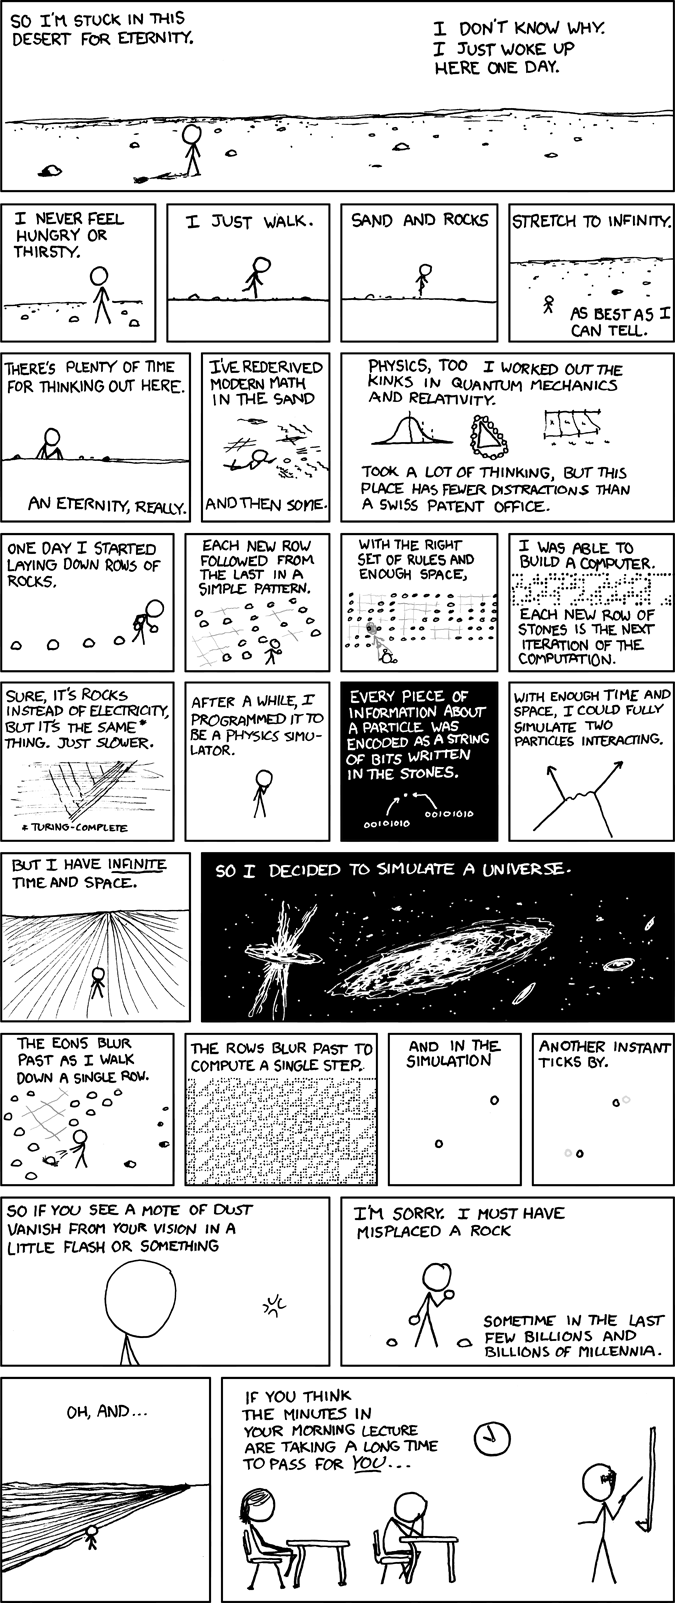
\includegraphics[width=0.7\textwidth]{./images/xkcd.png}\\
{source: \url{http://xkcd.com/505}}
}
\pagebreak

\chapter{A safe approximation of Kolmogorov complexity}
\label{chapter:safe}

\begin{abstract}
\noindent Kolmogorov complexity ($K$) is an incomputable function. It can be approximated from above but not to arbitrary given precision and it cannot be approximated from below. By restricting the source of the data to a specific model class, we can construct a computable function $\ok$ to approximate $K$ in a probabilistic sense: the probability that the error is greater than $k$ decays exponentially with $k$. We apply the same method to the normalized information distance (NID) and discuss conditions that affect the safety of the approximation.
\end{abstract}

\noindent The Kolmogorov complexity of an object is its shortest description, considering all computable descriptions. It has been described as ``the accepted absolute measure of information content of an individual object'' \cite{DBLP:journals/tit/GacsTV01}, and its investigation has spawned a slew of derived functions and analytical tools. Most of these tend to separate neatly into one of two categories: the platonic and the practical. 

On the platonic side, we find such tools as the normalized information distance \cite{DBLP:journals/tit/LiCLMV04}, algoritheoremic statistics \cite{DBLP:journals/tit/GacsTV01} and sophistication \cite{DBLP:journals/tit/Vitanyi06,adriaans2012facticity}. These subjects all deal with incomputable ``ideal'' functions: they optimize over all computable functions, but they cannot be computed themselves.

To construct practical applications (ie. runnable computer programs), the most common approach is to take one of these platonic, incomputable functions, derived from Kolmogorov complexity ($K$), and to approximate it by swapping $K$ out for a computable compressor like GZIP \cite{gailly1991gzip}. This approach has proved effective in the case of normalized information distance (NID) \cite{DBLP:journals/tit/LiCLMV04} and its approximation, the normalized compression distance (NCD) \cite{DBLP:journals/tit/CilibrasiV05}. Unfortunately, the switch to a general-purpose compressor leaves an analytical gap. We know that the compressor serves as an upper bound to $K$---up to a constant---but we do not know the difference between the two, and how this error affects the error of derived functions like the NCD. This can cause serious contradictions. For instance, the normalized information distance has been shown to be non-approximable \cite{DBLP:journals/jcss/TerwijnTV11}, yet the NCD has proved its merit empirically \cite{DBLP:journals/tit/CilibrasiV05}. Why this should be the case, and when this approach may fail has, to our knowledge, not yet been investigated.

We aim to provide the first tools to bridge this gap. We will define a computable function which can be said to approximate Kolmogorov complexity, with some practical limit to the error. To this end, we introduce two concepts:

\begin{itemize}
\item We generalize resource-bounded Kolmogorov complexity ($K^t$) to \emph{model-\\bounded Kolmogorov complexity}, which minimizes an object's description length over any given enumerable subset of Turing machines (a \emph{model class}). We explicitly assume that the source of the data is contained in the model class. 
\item We introduce a probabilistic notion of approximation. A function approximates another \emph{safely}, under a given distribution, if the probability of them differing by more than $k$ bits, decays at least exponentially in $k$. \footnotemark
\end{itemize}

\footnotetext{This consideration is subject to all the normal drawbacks of asymptotic approaches. For this reason, we have foregone the use of big-O notation as much as possible, in order to make the constants and their meaning explicit.} 

\noindent While the resource-bounded Kolmogorov complexity is computable in a technical sense, it is never computed practically. The generalization to model bounded Kolmogorov complexity creates a connection to \emph{minimum description length} (MDL) \cite{rissanen1978modeling,DBLP:journals/tit/Rissanen84,grunwald2007minimum}, which does produce algoritheorems and methods that are used in a practical manner. Kolmogorov complexity has long been seen as a kind of platonic ideal which MDL approximates. Our results show that MDL is not just an upper bound to $K$, it also approximates it in a probabilistic sense.

Interestingly, the model-bounded Kolmogorov complexity itself---the smallest description using a single element from the model class---is not a safe approximation. We can, however, construct a computable, safe approximation by taking into account all descriptions the model class provides for the data.

The main result of this paper is a computable function $\ok$ which, under a model assumption, safely approximates $K$ (Theorem~\ref{theorem:safe-computable}). We also investigate whether a $\ok$-based approximation of NID is safe, for different properties of the model class from which the data originated (Theorems \ref{theorem:unsafe-id}, \ref{theorem:safe-id} and \ref{theorem:safe-nid}).


\section{Turing Machines and Probability}

\subsection*{Turing Machines}

Let $\B= \{0, 1\}^*$. We assume that our data is encoded as a finite binary string. Specifically, the natural numbers can be associated to binary strings, for instance by the bijection: $(0, \epsilon)$, $(1, 0)$, $(2, 1)$, $(3, 00)$, $(4, 01)$, etc, where $\epsilon$ is the empty string. To simplify notation, we will sometimes conflate natural numbers and binary strings, implicitly using this ordering.

We fix a canonical prefix-free coding, denoted by $\overline{x}$, such that $|\overline{x}| \leq |x| + 2 \log{|x|}$. See \cite[Example~1.11.13]{DBLP:books/daglib/0087328} for an example . Among other things, this gives us a canonical pairing function to encode two strings $x$ and $y$ into one: $\overline{x}y$.

\noindent We use the Turing machine model from \cite[Example~3.1.1]{DBLP:books/daglib/0087328}. The following properties are important: the machine has a read-only, right-moving input tape, an auxiliary tape which is read-only and two-way, two read-write two-way worktapes and a read-write two-way output tape.\footnotemark~All tapes are one-way infinite. If a tape head moves off the tape or the machine reads beyond the length of the input, it enters an infinite loop. For the function computed by TM $i$ on input $p$ with auxiliary input $y$, we write $T_i(p\mid y)$ and $T_i(p) = T_i(p \mid \epsilon)$. The most important consequence of this construction is that the programs for which a machine with a given auxiliary input $y$ halts, form a prefix-free set \cite[Example~3.1.1]{DBLP:books/daglib/0087328}. This allows us to interpret the machine as a probability distribution (as described in the next subsection).

\footnotetext{Multiple work tapes are only required for proofs involving resource bounds.}

We fix an effective ordering $\{T_i\}$. We call the set of all Turing machines $\C$. There exists a universal Turing machine, which we will call $U$, that has the property that $U(\overline{\imath}p\mid y) = T_i(p\mid y)$ \cite[Theorem~3.1.1]{DBLP:books/daglib/0087328}. 

\subsection*{Probability}

We want to formalize the idea of a probability distribution that is \emph{computable}: it can be simulated or computed by a computational process. For this purpose, we will interpret a given Turing machine $T_q$ as a probability distribution $p_q$: each time the machine reads from the input tape, we provide it with a random bit. The Turing machine will either halt, read a finite number of bits without halting, or read an unbounded number of bits. $p_q(x)$ is the probability that this process halts and produces $x$: $p_q(x) = \sum_{p: T_q(p) = x} 2^{-|p|}$. We say that $T_q$ \emph{samples} $p_q$. Note that if $p$ is a semimeasure, $1-\sum_x p(x)$ corresponds to the probability that this sampling process will not halt.

We model the probability of $x$ conditional on $y$ by a Turing machine with $y$ on its auxiliary tape: $p_q(x \mid y) = \sum_{p : T_q(p|y) = x} 2^{-|p|}$.  

The \emph{lower semicomputable semimeasures} \cite[Chapter~4]{DBLP:books/daglib/0087328} are an alternative formalization. We show that it is equivalent to ours:

\renewcommand*{\thefootnote}{\fnsymbol{footnote}}

\begin{lemma}\footnotemark[2]
The set of probability distributions sampled by Turing machines in $\C$ is equivalent to the set of lower semicomputable semimeasures.
\label{lemma:sampling-equivalence}
\end{lemma}

\footnotetext[2]{Proof in the appendix.}

\noindent The distribution corresponding to the universal Turing machine $U$ is called $m$: $m(x) = \sum_{p: U(p) = x} 2^{-|p|}$. This is known as a universal distribution. $K$ and $m$ dominate each other, ie. $\exists c \forall x : |K(x) - \log m(x)| < c$ \cite[Theorem~4.3.3]{DBLP:books/daglib/0087328}.

\section{Model-Bounded Kolmogorov Complexity}

In this section we present a generalization of the notion of resource-bounded Kolmogorov complexity. We first review the unbounded version:

\begin{definition}
Let $k(x\mid y) = \argmin_{p:U(p\mid y) = x} |p|$. The prefix-free, conditional \emph{Kolmogorov complexity} is \begin{align*}
K(x\mid y) = |k(x\mid y)|
\end{align*} with $K(x) = K(x\mid \epsilon)$. \label{definition:kolmogorov-complexity}
\end{definition}
Due to the halting problem, $K$ is not computable. By limiting the set of Turing machines under consideration, we can create a computable approximation. 

\begin{definition}
A \emph{model class} $C \subseteq \C$ is a computably enumerable set of Turing machines. Its members are called \emph{models}. A \emph{universal model} for $C$ is a Turing machine $U^C$ such that $U^C(\overline{\imath}p\mid y) = T_i(p\mid y)$ where $i$ is an index over the elements of $C$. 
\end{definition}

\begin{definition}
For a given $C$ and $U^C$ we have $K^C(x) = \min \left \{|p| \;:\; U^C(p) = x \right \}$, called the \emph{model-bounded Kolmogorov complexity}.
\end{definition}
$K^C$, unlike $K$, depends heavily on the choice of enumeration of $C$. A notation like $K_{U^C}$ or $K^{i, C}$ would express this dependence better, but for the sake of clarity we will use $K^C$.

We define a model-bounded variant of $m$ as $m^C(x) = \sum_{p: U^C(p) = x} 2^{-|p|}$, which dominates all distributions in $C$:

\begin{lemma}
For any $T_q \in C$, $m^C(x) \geq c_q p_q(x)$ for some $c_q$ independent of $x$.
\label{lemma:universal-bounded-distribution}
\end{lemma}
\begin{proof}\belowdisplayskip=-12pt
\begin{align*}
m^C(x) = \sum_{i,p : U^C(\overline{\imath}p) = x} 2^{-|\overline{\imath}p|} 
\geq \sum_{p : U^C(\overline{q}p) = x} 2^{-|\overline{q}|}2^{-|p|} 
= 2^{-|\overline{q}|} p_q(x) \p
\end{align*}
\end{proof}

\noindent Unlike $K$ and $-\log m$, $K^C$ and $-\log m^C$ do not dominate one another. We can only show that $-\log m^C$ bounds $K^C$ from below ($\sum_{U^C(p)=x} 2^{-|p|} > 2^{-|k^C(x)|}$). In fact, as shown in Theorem~\ref{theorem:unsafe}, $-\log m^C$ and $K^C$ can differ by arbitrary amounts.

\renewcommand*{\thefootnote}{\arabic{footnote}}

\begin{example}[{resource-bounded Kolmogorov complexity \cite[Ch.~7]{DBLP:books/daglib/0087328}}]
\label{example:traditional-time-bounded}
\-\\ Let $t(n)$ be some time-constructible function.\footnotemark Let $T_i^t$ be the modification of $T_i \in \C$ such that at any point in the computation, it halts immediately if more than $k$ cells have been written to on the output tape and the number of steps that have passed is less than $t(k)$. In this case, whatever is on the output tape is taken as the output of the computation. If this situation does not occur, $T_i$ runs as normal. Let $U^t(\overline{\imath}p) = T^t_i(p)$. We call this model class $C^t$. We abbreviate $K^{C^t}$ as $K^t$. 

Since there is no known means of simulating $U^t$ within $t(n)$, we do not know whether $U^t \in C^t$. It can be run in $ct(n) \log t(n)$ \cite{DBLP:books/daglib/0087328,DBLP:journals/jacm/HennieS66}, so we do know that $U^t \in C^{ct\log t}$.
\end{example}

\footnotetext{Ie. $t: \N \rightarrow \N$ and $t$ can be computed in $O(t(n))$~\cite{DBLP:journals/mst/AntunesMSV09}.}

\noindent Other model classes include Deterministic Finite Automata, Markov Chains, or the exponential family (suitably discretized). These have all been thoroughly investigated in coding contexts in the field of Minimum Description Length \cite{grunwald2007minimum}.

\renewcommand*{\thefootnote}{\fnsymbol{footnote}}

\section{Safe Approximation}

When a code-length function like $K$ turns out to be incomputable, we may try to find a lower and upper bound, or to find a function which dominates it. Unfortunately, neither of these will help us. Such functions invariably turn out to be incomputable themselves \cite[Section~2.3]{DBLP:books/daglib/0087328}. 

To bridge the gap between incomputable and computable functions, we require a softer notion of approximation; one which states that errors of any size may occur, but that the larger errors are so unlikely, that they can be safely ignored: 

\begin{definition}
Let $f$ and $f_a$ be two functions. We take $f_a$ to be an approximation of $f$. We call the approximation \emph{$b$-safe (from above)} for a distribution (or \emph{adversary}) $p$ if for all $k$ and some $c > 0$: 
\[
p(f_a(x) - f(x) \geq k) \leq c b^{-k} \p
\] 
Since we focus on code-length functions, usually omit ``from above''. A \emph{safe} function is $b$-safe for some $b > 1$. An approximation is safe for a model class $C$ if it is safe for all $p_q$ with $T_q \in C$.
\label{definition:safety}
\end{definition}

\noindent While the definition requires this property to hold for all $k$, it actually suffices to show that it holds for $k$ above a constant, as we can freely scale $c$:

\begin{lemma}
If $\exists_{c} \forall_{k: k >k_0} : p(f_a(x) - f(x) \geq k) \leq c b^{-k}$, then $f_a$ is $b$-safe for $f$ against $p$. \label{lemma:k-zero}
\end{lemma}
\begin{proof}
First, we name the $k$ below $k_0$ for which the ratio between the bound and the probability is the greatest: $k_m = \argmax_{k\in [0, k_0]} \left[p(f_a(x) - f(x) \geq k)/cb^{-k}\right]$. We also define $b_m = cb^{-k_m}$ and $p_m = p(f_a(x) - f(x) \geq k_m)$. At $k_m$, we have $p(f_a(x) - f(x)\geq k_m) = p_m = \frac{p_m}{b_m}cb^{-k_m}$. In other words, the bound $c'b^{-k}$ with $c' = \frac{p_m}{b_m}c$ bounds $p$ at $k_m$, the point where it diverges the most from the old bound. Therefore, it must bound it at all other $k >0$ as well.
\end{proof}

\noindent Safe approximation, domination and lowerbounding form a hierarchy:

\begin{lemma}
Let $f_a$ and $f$ be code-length functions. If $f_a$ is a lower bound on $f$, it also dominates $f$. If $f_a$ dominates $f$, it is also a safe approximation.
\label{lemma:domination-safety}
\end{lemma}
\begin{proof}
Domination means that for all $x$: $f_a(x) - f(x) < c$, if $f_a$ is a lower bound, $c=0$. If $f_a$ dominates $f$ we have  
$\forall p, k > c : p(f_a(x) - f(x) \geq k) = 0$.
\end{proof}
Finally, we show that safe approximation is transitive, so we can chain together proofs of safe approximation; if we have several functions with each safe for the next, we know that the first is also safe for the last.

\begin{lemma}
The property of safety is transitive over the space of functions from $\mathbb B$ to $\mathbb B$ for a fixed adversary.
\label{lemma:reflexitvity}
\end{lemma}
\begin{proof} Let $f$, $g$ and $h$ be functions such that 
\begin{align*}
p(f(x) - g(x) \geq k) &\leq c_1{b_1}^{-k} \text{ and}\\
p(g(x) - h(x) \geq k) &\leq c_2{b_2}^{-k} \p
\end{align*}
We need to show that $p(f(x) - h(x) \geq k)$ decays exponentially with $k$. We start with
\begin{align*}
p\left(f(x) - g(x) \geq k \vee g(x) - h(x) \geq k\right)\;&\leq\;c_1{b_1}^{-k} + c_2{b_2}^{-k}\p
\end{align*}
$\left\{x : f(x) - h(x) \geq 2k\right\}$ is a subset of $\left\{x : f(x) - g(x) \geq k\vee g(x) - h(x) \geq k\right\}$, so that the probability of the first set is less than that of the second:
\begin{align*}
p\left(f(x) - h(x) \geq 2k\right) \leq c_1{b_1}^{-k} + c_2{b_2}^{-k} \p
\end{align*}
Which gives us \belowdisplayskip=-12pt
\begin{align*}
&p\left(f(x) - h(x) \geq 2k\right)\leq cb^{-k} \quad&& \text{with $b=\min(b_1, b_2)$ and $c = \max(c_1, c_2)$} \;,\\
&p\left(f(x) - h(x) \geq k'\right)\leq cb'^{-k'} \quad&& \text{with $b'=\sqrt{b}$}\p
\end{align*} 
\end{proof}

\section{A Safe, Computable Approximation of $K$}

\begin{figure*}[tb]
  \centering
  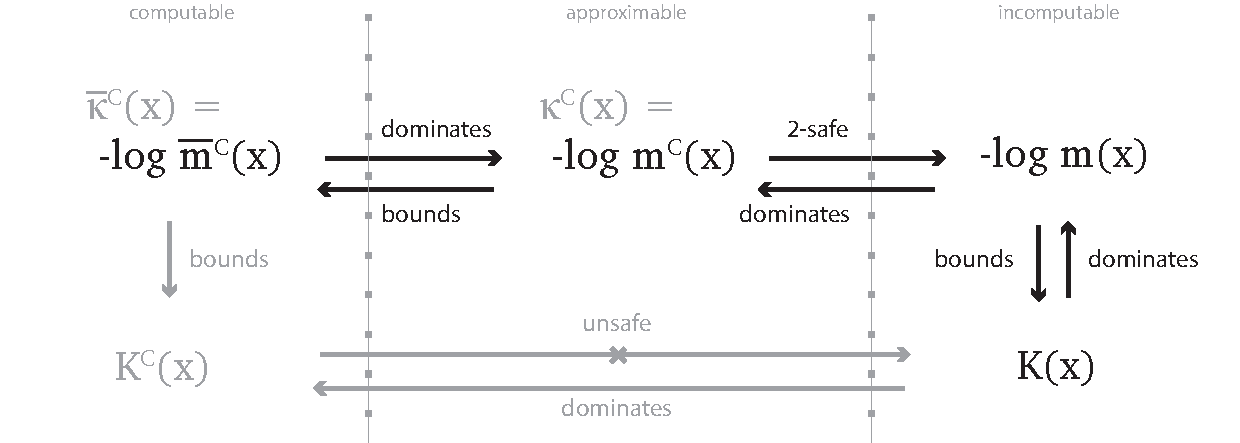
\includegraphics[width=\textwidth]{./images/approximation-map.pdf}
  \caption{\small An overview of how various code-length functions relate to each other in terms of approximation safety. These relations hold under the assumption that the data is generated by a distribution in $C$ and that $C$ is sufficient and complete.}
  \label{fig:approximation-map}
\end{figure*}

Assuming that our data is produced from a model in $C$, can we construct a computable function which is safe for $K$? An obvious first choice is $K^C$. For it to be computable, we would normally ensure that all programs for all models in $C$ halt. Since the halting programs form a prefix-free set, this is impossible. There is however a property for prefix-free functions that is analogous. We call this \emph{sufficiency}:

\begin{definition}
A sufficient model $T$ is a model for which every infinite binary string contains a halting program as a prefix. A \emph{sufficient model class} contains only sufficient models. 
\end{definition}
We can therefore enumerate all inputs for $U^C$ from short to long in series to find $k^C(x)$, so long as $C$ is sufficient. For each input, $U^C$ either halts or attempts to read beyond the length of the input. 

In certain cases, we also require that $C$ can represent all $x \in \B$ (ie. $m^C(x)$ is never 0). We call this property \emph{completeness}:
\begin{definition}
A model class $C$ is called \emph{complete} if for any $x$, there is at least one $p$ such that $U^C(p) = x$. 
\end{definition}
We can now say, for instance, that $K^C$ is computable for sufficient $C$. Unfortunately, $K^C$ turns out to be unsafe:
\begin{theorem}
There exist model classes $C$ so that $K^C(x)$ is an unsafe approximation for $K(x)$ against some $p_q$ with $T_q \in C$.  \label{theorem:unsafe}
\end{theorem}
\begin{proof}
We first show that $K^C$ is unsafe for $-\log m^C$. 

Let $C$ contain a single Turing machine $T_q$ which outputs $x$ for any input of the form $\overline{x}p$ with $|p| = x$ and computes indefinitely for all other inputs.

$T_q$ samples from $p_q(x) = 2^{-|\overline{x}|}$, but it distributes each $x$'s probability mass uniformly over many programs much longer than $|\overline{x}|$.

This gives us $K^C(x) = |\overline{x}| + |p| = |\overline{x}| + x $ and $-\log m^C(x) = |\overline{x}|$, so that $K^C(x) + \log m^C(x) = x$. We get 
\begin{align*}
m^C&(K^C(x) + \log m^C(x) \geq k) = m^C(x \geq k) = \\
&\sum_{x : x \geq k} 2^{-|\overline{x}|} \geq \sum_{x : x \geq k} 2^{-2 \log x} \geq k^{-2}
\end{align*}
so that $K^C$ is unsafe for $-\log m^C$.

It remains to show that this implies that $K^C$ is unsafe for $K$. In Theorem~\ref{theorem:safe}, we prove that $-\log m^C$ is safe for $K$. Assuming that $K^C$ is safe for $K$ (which dominates $-\log m^C$) implies $K^C$ is safe for $-\log m^C$, which gives us a contradiction.
\end{proof}
Note that the use of a model class with a single model is for convenience only. The main requirement for $K^C$ to be unsafe is that the prefix tree of $U^C$'s programs distributes the probability mass for $x$ over many programs of similar length. The greater the difference between $K^C$ and $- \log m^C$, the greater the likelihood that $K^C$ is unsafe.

Our next candidate for a safe approximation of $K$ is $-\log m^C$. This time, we fare better. We first require the following lemma, called the \emph{no-hypercompression theorem} in \cite[p103]{grunwald2007minimum}:
\begin{lemma}
Let $p_q$ be a probability distribution. The corresponding code-length function, $-\log p_q$, is a $2$-safe approximation for any other code-length function against $p_q$. For any $p_r$ and $k>0$: $
p_q(-\log p_q(x) +  \log p_r(x) \geq k) \leq 2^{-k}$.
\label{lemma:no-hypercompression}
\end{lemma} 

\renewcommand*{\thefootnote}{\arabic{footnote}}

\begin{theorem}
$-\log m^C(x)$ is a 2-safe approximation of $K(x)$ against any adversary from $C$.
\label{theorem:safe}
\end{theorem}
\begin{proof}\belowdisplayskip=-12pt
Let $p_q$ be some adversary in $C$. We have 
\begin{align*}
p_q&(-\log m^C(x) - K(x) \geq k) \\ 
&\leq c m^C(-\log m^C(x) - K(x) \geq k) &\text{by Lemma~\ref{lemma:universal-bounded-distribution},} \\
&\leq c 2^{-k} &\text{by Lemma~\ref{lemma:no-hypercompression}.}
\end{align*}
\end{proof}
While we have shown $m^C$ to be safe for $K$, it may not be computable, even if $C$ is sufficient (since it is an infinite sum). We can, however, define an approximation, which, for sufficient $C$, is computable and dominates $m^C$.

\begin{definition}
\label{definition:algoritheorem}
Let the model class $D$ be the union of $C$ and some arbitrary sufficient and complete distribution from $\C$.

Let $\m^C_c(x)$ be the function computed by the following algoritheorem:
Dovetail the computation of all programs on $U^D(x)$ in cycles, so that in cycle $n$, the first $n$ programs are simulated for one further step. After each such step we consider the probability mass $s$ of all programs that have stopped (where each program $p$ contributes $2^{-|p|}$), and the probability mass $s_x$ of all programs that have stopped and produced $x$. We halt the dovetailing and output $s_x$ if $s_x > 0$ and the following stop condition is met:
\[
\frac{1-s}{s_x} \leq 2^c - 1 \p
\] 
\end{definition}
Note that if $C$ is sufficient so is $D$, so that $s$ goes to 1 and $s_x$ never decreases.  Since all programs halt, the stop condition must be reached. The addition of a complete model is required to ensure that $s_x$ does not remain $0$ indefinitely.

\begin{lemma}
If $C$ is sufficient, $\m^C_c(x)$ dominates $m^C$ with a constant multiplicative factor $2^{-c}$ (ie. their code-lengths differ by at most $c$ bits).
\label{lemma:overline-dominance}
\end{lemma}
\begin{proof}\belowdisplayskip=-12pt
We will first show that $\m^C_c$ dominates $m^D$. Note that when the computation of $\m^C_c$ halts, we have $\m^C_c(x) = s_x$ and $m^D(x) \leq s_x + (1 - s)$. This gives us:
\[
\frac{m^D(x)}{\m^C_c(x)} \leq 1 + \frac{1 - s}{s_x} \leq 2^{c} \p
\]
Since $C \subseteq D$, $m^D$ dominates $m^C$ (see Lemma~\ref{lemma:subset-dominance} in the appendix) and thus, $\m^C_c$ dominates $m^C$.
\end{proof}
The parameter $c$ in $\m^C_c$ allows us to tune the algoritheorem to trade off running time for a smaller constant of domination. We will usually omit it when it is not relevant to the context. 

Putting all this together, we have achieved our aim: 
\begin{theorem}
For a sufficient model class $C$, $-\log \overline{m}^C$ is a safe, computable approximation of $K(x)$ against any adversary from $C$
\label{theorem:safe-computable}
\end{theorem}
\begin{proof}
We have shown that, under these conditions, $-\log m^C$ safely approximates $-\log m$ which dominates $K$, and that $-\log \overline{m}^C$ dominates $-\log m^C$. Since domination implies safe approximation (Lemma~\ref{lemma:domination-safety}), and safe approximation is transitive (Lemma~\ref{lemma:reflexitvity}), we have proved the theorem.  
\end{proof}
Figure~\ref{fig:approximation-map} summarizes this chain of reasoning and other relations between the various code-length functions mentioned.

The negative logaritheorem of $m^C$ will be our go-to approximation of $K$, so we will abbreviate it with $\kappa$:
\begin{definition}
$\kappa^C(x) = -\log m^C(x)$ and $\ok^C(x) = -\log \m^C(x)$.
\end{definition}  
Finally, if we violate our model assumption we lose the property of safety. For adversaries outside $C$, we cannot be sure that $\kappa^C$ is safe:

\begin{theorem} 
There exist adversaries $p_q$ with $T_q \notin C$ for which neither $\kappa^C$ nor $\ok^C$ is a safe approximation of $K$. 
\label{theorem:unsafe-outside}
\end{theorem}
\begin{proof}
Consider the following algoritheorem for sampling from a computable distribution (which we will call $p_q$):
\begin{itemize}
\item Sample $n \in {\mathbb N}$ from some distribution $s(n)$ which decays polynomially. 
\item Loop over all $x$ of length $n$ return the first $x$ such that $\kappa^C(x) \geq n$. 
\end{itemize}
Note that at least one such $x$ must exist by a counting argument: if all $x$ of length $n$ have  $-\log \overline{m}^C(x) < n$ we have a code that assigns $2^n$ different strings to $2^n-1$ different codes.

For each $x$ sampled from $q$, we know that $\ok(x) \geq |x|$ and $K(x) \leq -\log p_q(x) + c_q$. Thus: 
\begin{align*}
p_q&(\ok^C(x) - K(x) \geq k) \;\geq\; p_q(|x| + \log p_q(x) - c_q \geq k) \\
&= p_q(|x| + \log s(|x|) - c_q \geq k) \;=\; \sum\nolimits_{n:n + \log s(n) - c_q \geq k} s(n)\p
\end{align*}
Let $n_0$ be the smallest $n$ for which $2n > n + \log s(n) - c_q$. For all $k > 2n_0$ we have \belowdisplayskip=-12pt
\begin{align*}
\sum\nolimits_{n:n + \log s(n) - c_q \geq k} s(n) \geq \sum\nolimits_{n: 2n \geq k} s(n) \geq s\left(\tfrac{1}{2} k\right)\p
\end{align*}
\end{proof}
For $C^t$ (as in Example~\ref{example:traditional-time-bounded}), we can sample the $p_q$ constructed in the proof in $O(2^n\cdot t(n))$. Thus, we know that $\kappa^t$ is safe for $K$ against adversaries from $C^t$, and we know that it is unsafe against $C^{2^t}$.
\section{Approximating Normalized Information Distance}

\begin{definition}[{\cite{DBLP:journals/tit/LiCLMV04,DBLP:journals/tit/CilibrasiV05}}]
The normalized information distance between two strings $x$ and $y$ is 
\[
\text{NID}(x, y) = \frac{\max \left [ K(x\mid y), K(y\mid x)\right ]}{\max \left [K(x), K(y)\right ]} \p
\]
\label{definition:nid}
\end{definition}
The information distance (ID) is the numerator of this function. The NID is neither lower nor upper semicomputable \cite{DBLP:journals/jcss/TerwijnTV11}. Here, we investigate whether we can safely approximate either function using $\kappa$. We define $\id^C$ and $\nid^C$ as the $\id$ and $\nid$ functions with $K$ replaced by $\ok^C$. We first show that, even if the adversary only combines functions and distributions in $C$, $\id^C$ may be an unsafe approximation.

\renewcommand*{\thefootnote}{\arabic{footnote}}
 
\begin{definition}\footnotemark
A function $f$ is a ($b$-safe) \emph{model-bounded one-way function} for $C$ if it is injective, and for some $b > 1$, some $c > 0$, all $q \in C$ and all $k$: 
\begin{align*}
p_q\left (\kappa^C(x) - \kappa^C\left(x\mid f(x)\right ) \geq k\right ) \leq cb^{-k} \p
\end{align*}
\label{definition:one-way}
\end{definition}

\footnotetext{This is similar to the Kolmogorov one-way function \cite[Definition~11]{DBLP:journals/mst/AntunesMPST13}.}
\renewcommand*{\thefootnote}{\fnsymbol{footnote}}

\begin{theorem}\footnotemark[2]
\label{theorem:unsafe-id}
Under the following assumptions:
\begin{itemize}
\item $C$ contains a model $T_0$, with $p_0(x) = 2^{-|x|}s(|x|)$, with $s$ a distribution on $\mathbb N$ which decays polynomially or slower,
\item there exists a model-bounded one-way function $f$ for $C$,
\item $C$ is \emph{normal}, ie. for some $c$ and all $x$: $\kappa^C(x) <  |\overline{x}| + c$
\end{itemize}
$\id^C$ is an unsafe approximation for $\id$ against an adversary $T_q$ which samples $x$ from $p_0$ and returns $\overline{x}f(x)$.
\end{theorem}
If $x$ and $y$ are sampled from $C$ independently, we can prove safety:

\begin{theorem}\footnotemark[2]
Let $T_q$ be a Turing machine which samples $x$ from $p_a$, $y$ from $p_b$ and returns $\overline{x}y$. If $T_a, T_b \in C$, $\id^C(x, y)$ is a safe approximation for $\id(x, y)$ against any such $T_q$.
\label{theorem:safe-id}    
\end{theorem}
The proof relies on two facts:
\begin{itemize}
  \item $\ok^C(x\mid y)$ is safe for $K(x\mid y)$ if $x$ and $y$ are generated this way.
  \item  Maximization is a \emph{safety preserving operation}: if we have two functions $f$ and $g$ with safe approximations $f_a$ and $g_a$, $\max(f_a(x), g_a(x))$ is a safe approximation of $\max(f(x), g(x))$.
\end{itemize} 
For \emph{normalized} information distance, which is dimensionless, the error $k$ in bits as we have used it so far does not mean much. Instead, we use  $f/f_a$ as a measure of approximation error, and we introduce an additional parameter $\epsilon$:

\begin{theorem}\footnotemark[2]
We can approximate $\nid$ with $\nid^C$ with the following bound:
\[
p_q\left(\frac{\nid(x, y)}{\nid^C(x, y)} \notin \left (1 - \frac{k}{c}, 1 + \frac{k}{c}\right ) \right) \leq c'b^{-k} + 2\epsilon
\]
with 
\begin{align*}
p_q(\text{\textnormal{ID}}^C(x, y) \geq c) \leq \epsilon \;\text{and}\; p_q\left(\max \left[\kappa^C(x), \kappa^C(y)\right] \geq c\right) \leq \epsilon
\end{align*}
for some $b > 1$ and $c' > 0$, assuming that $p_q$ samples $x$ and $y$ independently from models in $C$.
\label{theorem:safe-nid}
\end{theorem}

\section{Discussion}

We have provided a function $\ok^C(x)$ for a given model class $C$, which is computable if $C$ is sufficient. Under the assumption that $x$ is produced by a model from $C$, $\ok^C(x)$ approximates $K(x)$ in a probabilistic sense. We have also shown that $K^C(x)$ is not safe. Finally, we have given some insight into the conditions on $C$ and the adversary, which can affect the safety of NCD as an approximation to NID.

Since, as shown in Example~\ref{example:traditional-time-bounded}, resource-bounded Kolmogorov complexity is a variant of model-bounded Kolmogorov complexity, our results apply to $K^t$ as well: $K^t$ is not necessarily a safe approximation of $K$, even if the data can be sampled in $t$ and $\kappa^t$ \emph{is} safe if the data can be sampled in $t$. Whether $K^t$ is safe ultimately depends on whether a single shortest program dominates among the sum of all programs, as it does in the unbounded case.

For complex model classes, $\kappa^C$ may still be impractical to compute. In such cases, we may be able to continue the chain of safe approximation proofs. Ideally, we would show that a model which is only locally optimal, found by an iterative method like gradient descent, is still a safe approximation of $K$. Such proofs would truly close the circuit between the ideal world of Kolmogorov complexity and modern statistical practice.

\section{Appendix}
\renewcommand*{\thefootnote}{\arabic{footnote}} 

\subsection{Turing Machines and lsc. Probability Semimeasures (Lemma~\ref{lemma:sampling-equivalence})} 
\begin{definition}
A function $f : {\mathbb B} \rightarrow {\mathbb R}$ is \emph{lower semicomputable (lsc.)} iff there exists a total, computable two-argument function $f': {\mathbb B} \times {\mathbb N} \rightarrow \mathbb Q$ such that: $\lim_{i \rightarrow \infty} f'(x, i) = f(x)$ and  for all $i$, $f'(x, i + 1) \geq f'(x, i)$.
\label{definition:semicomputable}
\end{definition}

\begin{lemma}
If $f$ is an lsc. probability semimeasure, then there exists a a function $f^*(x, i)$ with the same properties of the function $f'$ from Definition~\ref{definition:semicomputable}, and the additional property that all values returned by $f^*$ have finite binary expansions.
\label{lemma:f-star}
\end{lemma}
\begin{proof}
Let $x_j$ represent $x \in {\mathbb D}$ truncated at the first $j$ bits of its binary expansion and $x^j$ the remainder. Let $f^*(x, i) = f'(x, i)_i$. Since $f'(x, i) - f^*(x, i)_i$ is a value with $i+1$ as the highest non-zero bit in its binary expansion, $\lim_{i\rightarrow \infty} f^*(x, i) = \lim f'(x, i) = f(x)$.
 
It remains to show that $f^*$ is nondecreasing in $i$. Let $x \geq y$. We will show that $x_j \geq y_j$, and thus $x_{j+1} \geq y_j$. If $x = y$ the result follows trivially. Otherwise, we have $x_j = x - x^j > y - x^j = y_j + y ^j - x^j \geq y_j - 2^{-j}$. Substituting $x = f'(x, i+1)$ and $y = f'(x,i)$ tells us that $f^*(x, i+1) \geq f^*(x, i)$
\end{proof}

\begin{theorem}
Any TM, $T_q$, samples from an lsc. probability semimeasure.\label{theorem:back}
\end{theorem}
\begin{proof}
We will define a program computing a function $p_q'(x, i)$ to approximate $p_q(x)$: Dovetail the computation of $T_q$ on all inputs $x \in \mathbb B$ for $i$ cycles.

Clearly this function is nondecreasing. To show that it goes to $p(x)$ with $i$, we first note that for a given $i_0$ there is a $j$ such that, $2^{-j-1} < p_q(x) - p_q(x, i_0) \leq 2^{-j}$. Let $\{p_i\}$ be an ordering of the programs producing $x$, by increasing length, that have not yet stopped at dovetailing cycle $i_0$. There is an $m$ such that $\sum_{i=1}^m 2^{-|p_i|} \geq 2^{-j-1}$, since $\sum_{i=1}^{\infty}2^{-|p_i|} > 2^{-j-i}$. Let $i_1$ be the dovetailing cycle for which the last program below $p_{m+1}$ halts. This gives us $p_q(x) - p_q(x, i_1) \leq 2^{-j-1}$. Thus, by induction, we can choose $i$ to make $p(x) - p'(x, i)$ arbitrarily small. 
\end{proof}

\begin{theorem}
Any lsc. probability semimeasure can be sampled by a TM.\label{theorem:forth}
\end{theorem}
\begin{proof}
Let $p(x)$ be an lsc. probability semimeasure and $p^*(x, i)$ as in Lemma~\ref{lemma:f-star}. We assume---without loss of generality---that $p^*(x, 0) = 0$. Consider the following algoritheorem:

\noindent\-\quad\textbf{initialize} $s \leftarrow \epsilon$, $r \leftarrow \epsilon$ \\
\-\quad \textbf{for} $c = 1, 2, \ldots$: \\
\-\quad\quad \textbf{for} $x \in \{b \in \B  : |b| \leq c\}$\\
\-\quad\quad\quad $d \leftarrow p^*(x, c-i+1) - p^*(x, c-i)$\\
\-\quad\quad\quad $s \leftarrow s + d$\\
\-\quad\quad\quad add a random bit to $r$ until it is as long as $s$\\
\-\quad\quad\quad \textbf{if} $r < s$ then return $x$ \\
 
\noindent The reader may verify that this program dovetails computation of $p^*(x,i)$ for increasing $i$ for all $x$; the variable $s$ contains the summed probability mass that has been encountered so far. Whenever s is incremented, mentally associate the interval $(s,s+d]$ with outcome $x$. Since $p^*(x,i)$ goes to $p(x)$ as $i$ increases, the summed length of the intervals associated with $x$ goes to $p(x)$ and $s$ itself goes to $\overline{s} = \sum_x p(x)$. We can therefore sample from $p$ by picking a number r that is uniformly random on $[0, 1]$ and returning the outcome associated with the interval containing $r$. Since $s$ must have finite length (due to the construction of $p^*$), we only need to know $r$ up to finite precision to be able to determine which interval it falls in; this allows us to generate $r$ on the fly. The algoritheorem halts unless $r$ falls in the interval $[\overline{s}, 1]$, which corresponds exactly to the deficiency of $p$: if $p$ is a semimeasure, we expect the non-halting probability of a TM sampling it to correspond to $1-\sum_x p(x)$.
\end{proof}
Theorems~\ref{theorem:back}~and~\ref{theorem:forth} combined prove that the class of distributions sampled by Turing machines equals the lower semicomputable semimeasures (Lemma~\ref{lemma:sampling-equivalence}).

\subsection{Domination of model class supersets}

\begin{lemma}
Let $C$ and $D$ be model classes. If $C \subseteq D$, then $m^D$ dominates $m^C$:
\begin{align*}
\frac{m^D(x)}{m^C(x)} \geq \alpha
\end{align*}
for some constant $\alpha$ independent of $x$.
\label{lemma:subset-dominance}
\end{lemma}
\begin{proof}
We can partition the models of $D$ into those belonging to $C$ and the rest, which we'll call $\overline{C}$. For any given enumeration of $D$, we get $m^D(x) = \alpha m^C(x) + (1-\alpha)m^{\overline{C}(x)}$. This gives us:
\begin{align*}
\frac{m^D(x)}{m^C(x)} = \alpha + (1-\alpha)\frac{m^{\overline{C}(x)}}{m^C(x)} \geq \alpha \p
\end{align*}
\end{proof}

\subsection{Unsafe Approximation of $\id$ (Theorem~\ref{theorem:unsafe-id})}

\begin{proof}
\begin{align*} 
p_q&\left({\id}^C(x, y) - \id(x, y) \geq k \right) = \\
 &p_0\left(\max\left[\ok^C(x \mid f(x)), \ok^C(f(x)\mid x)\right] - \max\left[K(x\mid f(x)), K(f(x)\mid x))\right] \geq k\right) \p\\
p_q&\left(|x| - {\id}^C(x, y) \geq 2k\right) \;\leq\; p_0\left(|x| - \ok^C(x \mid f(x)) \geq 2k\right)\\
&\leq \;p_0\left(|x| - \kappa^C(x) \geq k \,\lor\, \kappa^C(x) - \ok^C(x \mid f(x)) \geq k\right)\\
&\leq \;p_0\left(|x| - \kappa^C(x) \geq k \right) \;+\; p_0\left(\kappa^C(x) - \kappa^C(x \mid f(x)) \geq k\right) \;\leq\; 2^{-k} + cb^{-k} \p
\end{align*}
$K$ can invert $f(x)$, so 
\begin{align*}
\id(x, y) = \max\left[K(x\mid f(x)), K(f(x)\mid x)\right] = \max\left[|f^*|, |f^*_{\text{inv}}|\right] < c_f\end
{align*}
where $f^*$ and $f^*_{\text{inv}}$ are the shortest program to compute $f$ on $U$ and the shortest program to compute the inverse of $f$ on $U$ respectively. 
 
\begin{align*}
p_q&\left({\id}^C(x,y) - \id(x,y) \geq k\right) + p_q\left(|x| - {\id}^C(x,y) \geq k\right)\\
&\geq\; p_q\left({\id}^C(x, y) - \id(x, y) \geq k \lor|x| - {\id}^C(x, y) \geq k\right)\\
&\geq\; p_q\left(|x| - \id(x, y) \geq k \right) \geq\; p_0\left(|x| - c_f \geq k\right) = \sum\nolimits_{i \geq k- c_f} s(i)\p
\end{align*}
Which gives us:\belowdisplayskip=-12pt
\begin{align*}
p_q&\left({\id}^C(x,y) - \id(x,y) \geq k\right) \\
&\geq \; - p_q(|x| - {\id}^C \geq k) + \sum\nolimits_{i \geq k- |f|} s(i) \geq- cb^{-k} + \sum\nolimits_{i \geq k- |f|} s(i) \\
& \geq s(k-|f|) - cb^{-k} \geq c's(k) \quad\quad\text{for the right  $c'$.}
\end{align*}
\end{proof}

\begin{corollary}
Under the assumptions of Theorem~\ref{theorem:unsafe-id}, $\ok^C(x\mid y)$ is an unsafe approximation for $K(x\mid y)$ against $q$. 
\end{corollary}
\begin{proof}
Assuming $\ok^C$ is safe, then since $\max$ is safety-preserving (Lemma~\ref{lemma:safety-preserving}), $\id^C$ should be safe for $\id$. Since it isn't, $\ok^C$ cannot be safe.
\end{proof}

\subsection{Safe Approximation of $\id$ (Theorem~\ref{theorem:safe-id})}

\begin{lemma}
If $q$ samples $x$ and $y$ independently from models in $C$, then $\kappa^C(x\mid y)$ is a $2$-safe approximation of $-\log m(x\mid y)$ against $q$.
\label{lemma:conditional-safety}  
\end{lemma}
\begin{proof}\belowdisplayskip=-12pt
Let $q$ sample $x$ from $p_r$ and $y$ from $p_s$.
\begin{align*}
p_q&(-\log m^C(x\mid y)  + \log m(x\mid y) \geq k) 		&&= p_q(m(x \mid y) / m^C(x \mid y) \geq 2^k) \\ 
&\leq \; 2^{-k}E\left[m(x\mid y)/m^C(x\mid y)\right] 	&&= 2^{-k} \sum_{x, y} p_s(y)m(x \mid y) \frac{p_r(x)}{m^C(x\mid y)}  \\
&\leq \; c 2^{-k} \sum_{x, y} p_s(y)m(x \mid y) \frac{m^C(x\mid y)}{m^C(x\mid y)} &&\leq c 2^{-k} \sum_{x, y} p_s(y)m(x \mid y) \leq c 2^{-k}\p
\end{align*} 
\end{proof}
Since $m$ and $K$ mutually dominate, $- \log m^C$ is $2$-safe for $K(x\mid y)$, as is $\ok(x\mid y)$.

\begin{lemma}
If $f_a$ is safe for $f$ against $q$, and $g_a$ is safe for $g$ against $q$, then $\max (f_a, g_a)$ is safe for $\max (f, g)$ against $q$.\footnote{We will call such operations \emph{safety preserving}}

\label{lemma:safety-preserving} 
\end{lemma}
\begin{proof}\belowdisplayskip=-12pt
We first partition $\B$ into sets $A_k$ and $B_k$:

\begin{description}
\item[$A_k = \{x:f_a(x) - f(x) \geq k \lor g_a - g(x) \geq k \}$] Since both $f_a$ and $g_a$ are safe, we know that $p_q(A_k)$ will be bounded above by the sum of two inverse exponentials in $k$, which from a given $k_0$ is itself bounded by an exponential in $k$.

\item[$B_k = \{x:f_a(x) - f(x) < k \wedge g_a - g(x) < k \}$] We want to show that $B$ contains no strings with error over $k$. If, for a given $x$ the left and right $\max$ functions in $\max \left(f_a, g_a\right) - \max \left(f, g\right)$ select the outcome from matching  functions, and the error is below $k$ by definition. Assume then, that a different function is selected on each side. Without loss of generality, we can say that $\max(f_a, g_a) = f_a$ and $\max(f, g)= g$. This gives us: $\max(f_a, g_a) - \max(f, g) = f_a - g \leq f_a - f \leq k$.
\end{description}
We now have $p(B_k) = 0$ and $p(A_k) \leq cb^{-k}$, from which the theorem follows.
\end{proof}

\begin{corollary}
$\id^C$ is a safe approximation of $\id$ against sources that sample $x$ and $y$ independently from models in $C$.
\end{corollary}

\subsection{Safe approximation of $\nid$ (Theorem~\ref{theorem:safe-nid})}

\begin{lemma}
Let $f$ and $g$ be two functions, with $f_a$ and $g_a$ their safe approximations against adversary $p_q$. Let $h(x) = f(x)/g(x)$ and $h_a(x) = f_a(x)/g_a(x)$. Let $c > 1$ and $0 < \epsilon \ll 1$ be constants such that $p_q(f_a(x) \geq c) \leq \epsilon$ and $p_q(g_a(x) \geq c) \leq \epsilon$. We can show that for some $b > 1$ and $c > 0$
\[
p_q\left(\left|\frac{h(x)}{h_a(x)} - 1\right| \geq \frac{k}{c}\right) \leq cb^{-k} + 2\epsilon \p
\]
\end{lemma}
\begin{proof}
We will first prove the bound from above, using $f_a$'s safety, and then the bound from below using $g_a$'s safety. 
\begin{align*}
p_q&\left(\frac{h}{h_a} \leq 1 - \frac{k}{c}\right) \;\leq\; p_q\left(\frac{h}{h_a} \leq 1 - \frac{k}{c} \;\&\; c < f_a \right) + \epsilon \;\leq\; p_q\left(\frac{h}{h_a} \leq 1 - \frac{k}{f_a} \right) + \epsilon \\
 &= p_q\left(\frac{f}{f_a}\frac{g_a}{g} \leq 1 - \frac{k}{f_a} \right) + \epsilon \leq p_q\left(\frac{f}{f_a} \leq 1 - \frac{k}{f_a} \right) + \epsilon \\
 &= p_q\left(\frac{f + k}{f_a} \leq 1 \right) + \epsilon \;=\;p_q\left(f_a - f \geq k \right) + \epsilon \;\leq\; c_f{b_f}^{-k} + \epsilon\p
\end{align*}
The other bound we prove similarly. Combining the two, we get\belowdisplayskip=-12pt
\begin{align*}
p_q\left(h/h_a \notin \left(k/c - 1, k/c + 1\right)\right) \leq c_f{b_f}^{-k} + c_g{b_g}^{-k} + 2\epsilon \;\leq\; c'b'^{-k} + 2\epsilon \p
\end{align*}
\end{proof} 
Theorem~\ref{theorem:safe-nid} follows as a corollary.


\chapter{The problem of sophistication}

\begin{summary}
The material in this chapter was adapted from the paper \emph{Two problems for sophistication} \textbf{P. Bloem}, S. de rooij, P. Adriaans \emph{Algorithmic Learning Theory 2015, 379-394}
\end{summary}

Sophistication was proposed to complement Kolmogorov Complexity in areas where the latter does not chime with our intuition. The previous chapters have hopefully convinced you that Kolmogorov complexity formalizes very neatly the notion of how much information an object contains. Yet the objects that are the richest in information according to Kolmogorov complexity don't seem to us very interesting. They are the static you see on an old fashioned tv, the noise you hear on your car's radio when you try to find a station or simply the sequence of ones and zeroes generated by a coin-flipping game. 

\index{Sophistication}

These are not signals that are rich or valuable to us. What makes data interesting is a mixture of predictability and unexpectedness: melodies, language, plot twists. Images of rolling hills or city scapes. Most of these would probably have a Kolmogorov complexity somewhere in between a small constant and the full length of the raw data. However, not all data with moderate Kolmogorov complexity is interesting: simply bending a coin so that it lands heads more often than tails will create an utterly boring sequence, with medium compressibility. 

Is there some other way to separate the wheat from the chaff? Can we find some function, in the spirit of Kolmogorov complexity, that tells us which data is \emph{interesting}? Sophistication is one approach: it tells us to consider not the descriptive complexity of the whole data, but of the model alone. This make intuitive sense; all the boring data mentioned above may have highly complexity, but the models are all simple. Contrast this with the optimal compression of a movie: such a model should contain information about language, human anatomy, plot structure, human emotion, architecture, nature. All these concepts are patterns present in the data, and the shortest program on the universal Turing machine exploits all of them. It must have a highly complex model.    
  
Where the theory breaks down, as we discuss in this chapter, is the idea that this shortest program separates neatly into structure and noise: the structure placed into the Turing machine $T_i$ and the noise placed in its input $y$. As we saw earlier, there are programs with the universal Turing machine for a model, that place all the information in the input, and the length of this representation is equal to the Kolmogorov complexity.
 
\section{Sophistication}

Kolmogorov complexity gives us a sound definition of the amount of information contained in a binary string. It does not, however, capture what most people would consider complexity. For example, a sequence of a million coin flips will almost certainly have maximal Kolmogorov complexity, even though there is nothing complex about flipping a coin repeatedly. Many scholars have defined additional measures in the spirit of Kolmogorov complexity, aimed at quantifying not \emph{all} information in a binary string, but only the \emph{meaningful}. While this concept has been given many names, we use \emph{sophistication} as an umbrella term. In this paper, we investigate two serious problems with sophistication. We conclude with two arguments suggesting the problems are fundamental, explaining our belief that sophistication cannot be defined in a satisfactory manner.

The Kolmogorov complexity $C(x)$\footnote of a binary string $x$ is, informally, the length of the shortest computer program to print $x$. This length depends on the choice of programming language, but, by the invariance theorem \cite[Section~2.1]{li1993introduction}, only by a constant, independent of $x$. For sufficiently complex objects, the choice of programming language becomes irrelevant and Kolmogorov complexity becomes an \emph{objective} measure. A definition of sophistication $S(x)$ in the spirit of $C(x)$ should have similar guarantees:

\footnotetext{In previous chapters, we defined Kolmogorov complexity using strings that can only read their input left to right, \emph{prefix-free Turing machines}. Such Turing machines lead to the prefix-free Kolmogorov complexity $K(x)$. In this chapter, we also use the classical Kolmogorov complexity $C(x)$, defined on Turing machines that can read back an forth on their input tape at will. Since the sophistication knows many definitions, some using $C(x)$, some using $K(x)$, we must consider both variants.}

\begin{enumerate}
\item $S(x)$ should count the bits required for an effective description of the structural properties of a binary string.
\item An analogue of invariance should hold: there must be strict limits on how much sophistication can be affected by a change in programming language.
\item There should be no constant $c$ such that $S(x)\le c$ for every input $x$. If sophistication is bounded, then knowing its value under one programming language provides no constraints on its value under another language (except that it is also bounded). 
\item Similarly, there should be no constant $c$ such that $\left | C(x)-S(x)\right |\le c$ for all $x$, because then sophistication would be equivalent to Kolmogorov complexity. 
\end{enumerate}
There have been many proposals for such a measure, all based on a \emph{two-part code}: we encode a \emph{model} in the first part of the code, which is interpreted as a representation of $x$'s structural properties. The model does not fully specify $x$, but when combined with the second part of the code, which specifies the noise, the original string becomes fully determined.\footnotemark

\index{Sophistication!Required properties}\index{Two-part coding}
\footnotetext{Some variants deviate from the two-part coding format, see Section~\ref{section:other}.}

For any string $x$, there may be many different two-part codes. The total length can never be less than the Kolmogorov complexity, but it can come close. Figure~\ref{figure:diagram} illustrates the principle. The key to sophistication is to take the representations that come close to the Kolmogorov complexity, the \emph{candidates}, and define the sophistication as the size of the smallest model in this set. However, for most definitions, we can prove that they fail one of the conditions above. For others, we cannot \emph{prove} they conflict with our requirements, but we show these methods only assign substantial sophistication to strings that require an enormous amount of processing to construct. 

\begin{figure*}[tb]
  \vspace{-2\baselineskip}
  \centering
  \begin{minipage}{0.40\textwidth}
     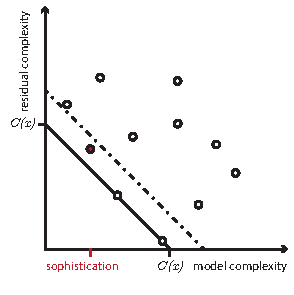
\includegraphics[width=\textwidth]{./images/sophistication.pdf}
  \end{minipage}
  \begin{minipage}{0.40\textwidth}
     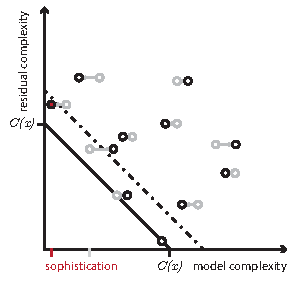
\includegraphics[width=\textwidth]{./images/sophistication-jump.pdf}
  \end{minipage}
  \caption{\small (left) Two-part representations of $x$ by the two components of their code. The Kolmogorov complexity $C(x)$, appearing as a black diagonal, provides a lower bound on the total codelength. We consider only representations that are close to this optimum---called \emph{candidates}---with the threshold represented by a dashed line. The size of the smallest model below the threshold is the sophistication of the data. (right) The same image, after a constant perturbation in the model complexity caused by a change in numbering.}
  \label{figure:diagram}
\end{figure*}\enlargethispage{3\baselineskip}

A valid definition of $S(x)$ must contend with two important issues. First, the details of the way the model is encoded are important. There are two technically distinct approaches; in one of these one has to deal with the so-called ``nickname problem'' that strangely remains unresolved in several publications. These definitions yield a sophistication that is highly dependent on the chosen programming language, unless special care is taken, as discussed in Section~\ref{section:indices}.

The second issue is that of striking the right balance between under- and overfitting, which we consider in Section~\ref{section:balance}. Overfitting is a common problem in statistics, that refers to the tendency to choose a complex model that provides a very good fit to the observed data, but does not generalise well to unseen data. In the case of sophistication, overfitting occurs if the model that determines the sophistication contains much or even all of the noise. In statistics, overfitting is often addressed by penalising complex models. In sophistication, however, such penalties tend to break the balance between structural information and noise, and lead to the opposite problem: underfitting.

\index{Overfitting}

Underfitting occurs when the selected model is simple, but fails to capture all structure in the data. This is also a problem for sophistication because the models under consideration are so powerful. In particular, in any programming language, there are programs that implement an interpreter for \emph{another} language. Such \emph{universal models} are \emph{simple}, since they can be described with a relatively small number of bits, yet are able to represent any data using a code within a constant from the Kolmogorov complexity. Such a two-part representation essentially encodes all information as noise. If complex models are penalized, then the problem becomes to make sure that universal models are not \emph{always} preferred for complex data. The usual workaround is to restrict the set of allowed models, for instance to total functions. While this excludes universal models, it is questionable whether it adequately solves the problem of underfitting in general.
\index{Underfitting}

Finally, in Section~\ref{section:conclusion} we argue that while two-part coding can yield useful insights into the structure of the data and identifies some models as poor representations, it is probably not possible to objectively separate structure from noise and identify a \emph{single} model as ``best'': many models of different complexities may be reasonable representations. Rather than doggedly trying to ``fix'' this property of algorithmic statistics, we propose embracing the idea that the data allows for multiple, equivalent interpretations of which information is structured, and which is random, and that there is no such thing as sophistication.

\section{Notation}

The following notation allows us to generalize across all definitions and variants of sophistication, save the occasional exception which we will highlight individually.

In the last chapter we dealt with Turing machines and conflated them with the functions they compute. In this chapter, we will focus more strongly on the functions themselves. A \emph{partial computable function} is one that is computable by Turing machine. We consider non-prefix-free Turing machines as well (the prefix-free Turing machines are a subset of these). 

We deal with partial computable functions $f: \B \times \B \to \B$, which we also call \emph{models}. $f$ is called \emph{prefix} if $\text{dom}_z(f)~=~\{y~:~f(y,~z)~\neq \infty\}$, is a prefix free set for all $z$, i.e. no string in $\text{dom}_z(f)$ is a prefix of another. A function $f$ is \emph{total} if $\forall_z \text{dom}_z(f) = \B$. In most cases, we do not use the second argument, and let $f(x) = f(x, \epsilon)$.

A \emph{numbering} is an enumeration of the partial computable functions, denoted by $\psi_1, \psi_2, \ldots$ or simply $\psi$. We fix one canonical numbering $\phi$, chosen to be \emph{effective}: ie. given $i$ and $y$, we can effectively compute $\phi_i(y)$. We call a numbering $\psi$ \emph{acceptable} if there exist total, computable functions $a, b: \N \to \N$ with $\forall: i$, $\phi_i = \psi_{b(i)}$ and  $\psi_i = \phi_{a(i)}$. One example of an effective, acceptable numbering is to take descriptions of Turing machines (by some standard scheme), first by length, and then lexicographically. The rank in this ordering corresponds to the number in the numbering.

\index{Numbering}\index{Acceptable numbering}\index{Numbering!Acceptable}

We generalize the definition of a model class. A \emph{generic model class} is a set of indices in a numbering $\psi$. We define four classes:
\begin{itemize} 
  \item The indices of the partial computable functions $\C=\N$.
  \item The total functions $\T=\{i:\tn{$\psi_i$ is total}\}$. Note that $\T$ is not computably enumerable.
  \item $\K$ is an enumerable set such that $\{\psi_i:i\in\K\}$ is the set of all partial computable prefix functions.
  \item The finite sets: $\F$ is an enumerable set such that $\{\psi_i:i\in\F\}$ is the set of uniform codes for all finite sets.\footnote{A uniform code for a set $F$ is a surjective prefix function $f:\{0,1\}^{\lceil\log|F|\rceil}\to F$.}
\end{itemize}
The model class $\T$ highlights the contrast with the \emph{effective} model classes of the last chapter: $\T$ is not-enumerable. All model classes in this chapter are generic, and we will omit the adjective in the remainder.

For technical reasons, we deviate slightly from the traditional notation of Kolmogorov complexity used in the last chapter: let $\M$ be a model class and $\psi$ an acceptable numbering, then let $C^{\M,\psi}(x\mid z)=\min\{|\bar\imath y|:\psi_i(y, z)=x,i\in\M\}$, with $C^{\M,\psi}(x) = C^{\M,\psi}(x\mid \epsilon)$. We omit the numbering when the distinction is not relevant. 

$C^\C(x)$ corresponds to the plain Kolmogorov complexity $C(x)$. $C^\K(x)$ corresponds to the prefix-free version $K(x)$ from te last chapter. This is a different construction, but it can be shown that the two are equal up to a constant.

Note that the notation $C^{\{i\}, \psi}(x)$ can be used to represent the smallest two-part description of $x$ using model $\psi_i$.

In these constructions we have used the principle of a numbering for the purpose normally served by the universal Turing machine: it captures the ad-hoc and subjective choices made in the construction of the Kolmogorov complexity, and by extension, the sophistication.

We prefer to work with numberings as it highlights an important issue: while Kolmogorov complexity is invariant to the choice of numbering this property does not immediately carry over to sophistication: for some treatments, the result is highly dependent on the chosen numbering, as we will see in the next section. 
 
\section{Inefficient indices}
\label{section:indices}

The simplest approach to sophistication would be to `open up' the Kolmogorov complexity and to see which program achieves the smallest description length: the program that \emph{witnesses} the Kolmogorov complexity. This witness is a two-part coding; it consists of a model and an input.

\index{Witness}\index{Two-part coding}

\begin{definition}[Index sophistication]
Let $\psi$ be an acceptable numbering. Let $\M$ be the model class from which candidates are chosen, and let $\Nm$ be the model class that determines the minimum achievable complexity. Let $c$ be a fixed constant. The \emph{index sophistication} is:
\[
\s_{\tn{index}}^{\M,\Nm,\psi,c}(x) = \min\left\{ |i| : C^{\{i\}, \psi}(x) \leq C^{\Nm, \psi}(x)+c,\;i \in \M\right\} \p
\]
When $\M = \Nm$, we will use $\s_\tn{index}^{\M,\psi,c}$. If the set over which the minimum is taken is empty, the sophistication is undefined.\label{definition:index}
\end{definition}
Koppel and Atlan's treatment \cite{koppelSoph1988,koppel1991almost}, where the name \emph{sophistication} originates, follows this basic logic, although it contains idiosyncracies like the use of monotonic models, and an extension to infinite strings. As the subsequent history of sophistication has discarded these, we will not discuss them here.

\index{Sophistication!Koppel and Atlan's}

In \cite{antunes2009sophistication,antunes2013sophistication} Koppel's principle is limited to finite strings, with $\T$ as a model class. The definition is similar to $S_\tn{index}^{\T, \C,\psi,c}$, except the total complexity of a witness $(i,y)$ is measured as $|i|+|y|$ without the cost of delimiting the two. This difference is not relevant to the current discussion. The restriction to $\T$ is a common approach, which avoids underfitting, as discussed in the next section.
 
\index{Sophistication!Antunes'}

\begin{lemma}\label{lemma:perverse}
Let $\s_\tn{index}^\psi$ denote any index sophistication with respect to numbering $\psi$ (with any choice for $\M$, $\Nm$ and $c$). There are acceptable numberings $\psi$ and $\xi$ such that for all $x$: $|\s_\tn{index}^\psi(x) - \s_\tn{index}^\xi(x)|\geq \tfrac{1}{2}\min\{\s_\tn{index}^\psi(x),\s_\tn{index}^\xi(x)\}$.
\end{lemma}
\begin{proof}
Let $z_i \in \B$ consist of $2^{i}-1$ zeroes followed by a one. Define $\psi, \xi$ such that $\psi_j(x) = \phi_i(x)$ for $j = z_{2i}$ and $\xi_j(x) = \phi_i(x)$ for $j = z_{2i+1}$, with all other functions returning $\infty$ for all inputs. Choose any $x$ and assume w.l.o.g. that $\s_\text{index}^\psi(x)\le \s_\text{index}^\xi(x)$. By construction, we have $2\s_\text{index}^\psi(x)  \leq \s_\text{index}^\xi(x)$.
\end{proof}
Thus, the length of the index is a very poor indicator of model complexity. For a robust measure, we define the complexity of a function $f$ as in \cite{grunwald2004shannon,vitanyi2004meaningful} by 
\begin{align}
C^{\M,\psi}(f) = \min\{C^{\M,\psi}(i):\psi_i=f\} \p \label{equation:function-complexity}
\end{align}
Lemma~\ref{lemma:invariance} in the appendix shows that $C^\C(f)$ and $C^\K(f)$ are invariant. 

Note that the perversely inefficient numberings of Lemma~\ref{lemma:perverse} are no issue for Kolmogorov complexity: we can use a UTM with a more efficient numbering as a model at only a constant penalty. For sophistication, however, the numbering is crucial.

There are two ways to use $C^\M(f)$ for more robust attempts to define sophistication. Confusingly, both are used in the literature. First, we can measure the complexity of the \emph{model} $\phi_i$ as $C^\K(\phi_i)$, which is then the size of the first part of a two-part code describing the data. This approach is used in  \cite{cover1985kolmogorov,gacs2001algorithmic,vitanyi2004meaningful,gellmann1996information}.

Second, we can stick to using the length of the index as the measure of sophistication, but restrict the allowed numberings to those that can represent a given function \emph{efficiently}. This approach is taken by Adriaans in \cite{adriaans2012facticity}, who defines \emph{facticity} as $\s_\text{index}^{\C,\psi,0}$, but only allows \emph{faithful} numberings. Formally, a faithful numbering has the property that $\forall i \exists j : \psi_i=\psi_j, |j|\le C^{\C}(\psi_j)+c$, for some constant $c$. Essentially, this means that a faithful numbering can represent a function $f$ with an index the same length as the Kolmogorov complexity $C^\C(f)$.

\index{Facticity}

Contrary to Adriaans' suggestion, there do actually exist faithful, acceptable numberings:

\begin{lemma}\label{lemma:faithful-numberings}
  There are faithful acceptable numberings.
\end{lemma}
\index{Numbering!Faithful}

\begin{proof}
Let $d \in \N$ be an index such that $\phi_d(y)=\infty$ for all $y$. Define
\[
\psi_q=\begin{cases}
\phi_{\phi_i(p)}&\tn{if $q$ can be written as $\bar\imath p$ and $\phi_i(p)<\infty$,}\\
\phi_d&\tn{otherwise.}\end{cases}
\]
It may seem that the second line requires a test whether $\phi_i(p)$ halts, for $\psi$ to be acceptable, but as we will show below, this is not the case.  
  
To show that $\psi$ is faithful, pick any function $f$. Then
\[\begin{split}
C^{\C, \phi}(f)&=\min\{C^{\C, \phi}(i):\phi_i=f\} =\min\{\min\{|\bar a b|:\phi_a(b)=i\}:\phi_i=f\} \\
& =\min\{|\bar a b|:\phi_{\phi_a(b)}=f\}
 =\min\{|\bar a b|:\psi_{\bar a b}=f\}.
\end{split}\]
This shows there is a sufficiently small $\psi$ index.

To show that $\psi$ is acceptable, let $\phi_j(z)=z$. Then a $\phi$-index $i$ can be mapped to a $\psi$-index
with $r(i)=\bar\jmath i$, so that
$\psi_{r(i)}(y)=\psi_{\bar\jmath i}(y)=\phi_i(y)$. For the reverse,
define $\phi_v(\bar\imath p, y)=\phi_{\phi_i(p)}(y)$. For fixed
$\bar\imath p$, the 
$s^n_m$-theorem \cite{kleene193notation} states that we can compute the $h$
such that $\phi_h(y)=\phi_v(\bar\imath p,y)$. Let $h(\bar\imath p)$
denote this index as a function of the program; further define
$h(q)=d$ if $q$ cannot be expressed as $\bar\imath p$. By
construction $h$ is total and computable. To check that the mapping
returns the correct function, rewrite $\phi_{h(\bar\imath
  p)}(y)=\phi_v(\bar\imath p,y)=\phi_{\phi_i(p)}(y)=\psi_{\bar\imath p}(y)$.
Note that if $q$ can be written as $\bar \imath p$, but $\phi_i(p)$ diverges, $h(q)$ will still return a function, but one which doesn't halt, making it equivalent to $\phi_d$ as required. 
\end{proof}

However, even choosing a faithful numbering is not enough. The Kolmogorov complexity uses representations of the form $\bar\imath y$, with $\psi_i(y) = x$,  where the bar denotes some straightforward prefix encoding to delimit the model description $i$ from its input $y$. If we define a second prefix encoding $\tilde{\imath}$, with $|\bar\imath|-|\tilde\imath|$ unbounded, we can define a second representation $\bar u \tilde \imath y$, with $\psi_u(\tilde{\imath} y) = \psi_i(y)$, at a constant overhead $|\br{u}|$, and gain more than $|\br{u}|$ for sufficiently complex strings, resulting again in a bounded sophistication.

We continue with a sophistication that avoids the issues of inefficient indices and of inefficient prefix encodings. We change the definition of index sophistication so that its two-part representations use $C^\K(\phi_i)$ bits for the representation of the model. We first introduce the following notation for the $\M$-Kolmogorov complexity using such compact two-part representations:
\[
\Cc^{\M, \psi}(x) = \min\{ C^{\K, \psi}(\psi_i) + |y| :  \psi_i(y) = x, i \in \M\}\p
\]
For model classes $\K$ and $\C$ this is equivalent to the existing definition and invariant to the numbering. Note that again, we use $\Cc^{\{i\}, \psi}(x)$ to represent the smallest two-part code using model $\psi_i$.

\begin{definition}[Sophistication]
\[
S^{\M,\Nm,\psi,c}(x)=\min\left\{C^\K(\phi_i): \Cc^{\{i\}, \psi} \le \Cc^{\Nm,\psi}(x)+c, i\in\M\right\}.
\]
\end{definition}

\section{Balancing under- and overfitting}
\label{section:balance}

In the last section, we began to see the delicate balance between the two code components. We will study this balance, starting with the variant $S^{\K,\psi,c}$, which is not used in the literature, but helps to illustrate the issues we wish to discuss.

$\K$ has optimal representations with all but a constant part of the information in the input and it has optimal representations with all information in the model. The downside to this balance is that it becomes easy to show a lack of invariance. We can tweak the numbering so that models in a specific subset $\M'\subset\K$ become cheaper to represent by an arbitrary amount relative to others: we can ensure that a model in $\M'$ always determines the sophistication. For instance, if we let $\M'$ contain only a universal model we get a bounded sophistication.

\begin{theorem}[Underfitting]
Let $\M, \Nm$ be model classes with $\M \subseteq \Nm$ and let $\M$ contain a universal model $\phi_u$, with the property that $\exists c \forall i \in \Nm, x \in \B : \Cc^{\{u\},\phi}(x) \leq \Cc^{\Nm, \phi}(x)+ c$. Then, for some numbering $\psi$, $S^{\M,\Nm, \psi,c}$ is bounded. \label{theorem:underfitting}
\end{theorem}
This problem is well known and many treatments avoid it by restricting the model class. Less well known, perhaps, is that the same holds in the other direction:  if $\M'$ is the set of \emph{singleton} models---those models that output a single $x$ for an empty input---we get a sophistication equal to the Kolmogorov complexity.

\begin{theorem}[Overfitting]
Let $\X \subseteq \B$. Let $\M \subseteq \Nm \subseteq \K$ be model classes where for every $x\in\X$ there is a singleton model $i\in\M$ with $\phi_i(\epsilon)=x$. Then there is a numbering $\psi$, and a constant $c$, such that for all $x\in\X$ we have $C^\K(x)-S^{\M,\Nm,\psi,c}(x) \leq c$.\label{theorem:overfitting}
\end{theorem}
The proofs of both theorems rely on a simple principle: there exist numberings which have the effect of penalizing $C^\K(\phi_i)$ for any model outside $\M'$ by an arbitrary constant amount. We can use this to effectively `push' these models outside of the range of candidates, ensuring that, under this numbering, a model in $\M'$ always determines the sophistication. The requirements for $\M'$ are somewhat complex. The following lemma gives a set of sufficient conditions.

\begin{lemma}
\label{lemma:thecoolone}
Let $\M$ and $\Nm$ be any model class, let $\X$ be any set of binary strings and let $D:\B\to\N$ be a partial computable decoding function with a prefix-free domain that maps function descriptions to their indices in $\phi$. Let $\M'= \tn{range}(D)$. Further assume there is a constant $c$ such that:\\
\-\hspace{1cm}(a) $\forall_{m\in\M'}:\min\{|p|:\phi_{D(p)}=\phi_m\}\le C^{\K,\phi}(\phi_m)+c$\\
\-\hspace{1cm}(b) $\forall_{x\in\X}: \Cc^{\M', \phi}(x) - \Cc^{\Nm, \phi}(x) \le c$.\\
Then, there is a $\psi$ such that if $S^{\M,\Nm,\psi,k}(x)$ is defined, then $S^{\M,\Nm,\psi,k}(x) = S^{\M',\Nm,\psi,k}(x)$ up to a constant. 
\end{lemma}
\begin{proof}\enlargethispage{2\baselineskip}
Pick any $x \in \X$. Let $f$ and $g$ be $\phi$-indices such that $f \in \M'$ and $g \notin \M'$ nor is $\phi_g$ equivalent to any function indexed by $\M'$. Furthermore let $\Cc^{\{f\}, \phi}(x)$ and $\Cc^{\{g\}, \phi}(x)$ both be within a constant $q$ of $\Cc^{\Nm,\phi}(x)$. Assumption (b) ensures that $\M'$ always provides such an $f$. 

We will show that for every integer $r$, there is a numbering $\psi$ such that $\Cc^{\{g'\}, \psi}(x) - \Cc^{\{f'\}, \psi}(x) \geq r$ for all $x \in \X$, where $f'$ and $g'$ are the $\psi$-indices equivalent to $f$ and $g$. Thus, for large enough $r$, $\phi_g$ is eliminated as a candidate model, while $\phi_f$ remains in place. Thus, under $\psi$, a member of $\M'$ determines the sophistication, or the sophistication is undefined.

Let $d$ be a positive constant. We will show later how to choose it to achieve the required result. We define $\psi$ as follows:
\[
\psi_0(p) = 0^d 1 D(p), \;\;\;
\psi_{0^d1i}(p) = \phi_i(p), \;\;\;
\psi_j(\cdot) = \infty \;\text{if $j\neq 0$ and $j \neq 0^d1\ldots$}
\]
The key to the proof is the way that the function complexity $C^\K(\cdot)$ changes when we change the numbering from $\phi$ to $\psi$. For $f$, the value increases by no more than a fixed constant, but for $g$, it increases by a constant that we can arbitrarily increase by increasing $d$.

We will first show that for $f$, the value does not increase by more than a constant $c_f$. Assume w.l.o.g. that $0 \in \K$.
\begin{align*}
C^{\K, \psi}(\phi_f) &= \min\left\{|\bar \jmath q| : \psi_{\psi_j(q)} = \phi_f, j \in \K \right\} & \text{rewriting (\ref{equation:function-complexity})} \\
&\leq \min \left\{ |\overline{0} q| : \psi_{\psi_0(q)} = \phi_f \right\}& \text{choose $j=0$} \\
&= \min \left\{ |q| : \phi_{D(q)} = \phi_f \right\} + |\overline{0}| \\
&\leq C^{\K, \phi}(\phi_f) + c_f & \text{by assumption (a).}
\end{align*}
In order to show that for $g$, we can increase the difference by an arbitrary constant, we first show that, for any $z$ not in the range of $\psi_0$, the Kolmogorov complexity itself increases by at least $d$ when we switch from $\phi$ to $\psi$:
\begin{align}
C^{\K, \psi}(z) &= \min\left\{|\bi y| : \psi_i(y) = z, i \in \K \right\} & \text{by definition}\nonumber\\
&= \min\left\{|\overline{0^d1j} y| : \psi_{0^d1j}(y) = z \right\} & \text{since $z\notin \text{range}(\psi_0)$} \nonumber\\
&\geq \min\left\{|\bar \jmath y| : \phi_{j}(y) = z \right\} + d &\nonumber\\
&= C^{\K, \phi}(z) + d\p & \label{line:kolmogorov-switch}
\end{align}
We now show the increase in model complexity for $g$. First, assume $\phi_g \neq \psi_0$:
\begin{align*}
C^{\K,\psi}(\phi_g) &= \min \left\{C^{\K, \psi}(i) : \psi_i = \phi_g \right\} \\
&= \min \left\{C^{\K, \psi}(0^d1j) : \phi_j = \phi_g \right\} \\
&= C^{\K, \psi}(0^d1j) \\
&\geq C^{\K,\phi}(0^d1j) + d & \text{by (\ref{line:kolmogorov-switch})} \\
&\geq C^{\K,\phi}(j) - c_g + d &\text{since $C^\K(j) \leq C^\K(0^d1j) + c_0$}\\
&\geq C^{\K, \phi}(\phi_g) - c_g + d \p
\end{align*}
Now assume $\phi_g = \psi_0$. We have $C^{\K,\psi}(\phi_g) = \min\left\{C^{\K, \psi}(i) : \psi_i = \psi_0 \right\} \geq d$. This follows from the fact that the minimum is achieved either at $i = 0$ or at $i = 0^d1m$ with $m \notin \M'$. Neither have a representation using a function with a $\psi$-index without the $0^d1$ prefix.

Choosing $d \geq r + \max \left\{C^{\K,\phi}(\psi_0), c_g \right\} + c_f + 2q$ ensures that for both cases, we have $C^{\K, \psi}(\phi_g) \geq C^{\K, \phi}(\phi_g) + r + c_f + 2q$. While $C^\K(\psi_0)$ depends on the choice of $d$, we have $C^\K(\psi_0) \leq C^\K(d) + C^\K(D)$, up to a constant, which is in $O(\log d)$, so we can choose $d$ to satisfy the inequality.  

Finally, we can show the result: \belowdisplayskip=-26pt
\begin{align*}
&\Cc^{\{g'\}, \psi}(x) - \Cc^{\{f'\}, \psi}(x)\\
&=C^{\K, \psi}(\phi_g) + \min\{|y| : \phi_g(y) = x\} - C^{\K, \psi}(\phi_f) - \min\{|y| : \phi_f(y) = x\}\\
&\geq C^{\K, \phi}(\phi_g) + r + c_f + 2q + \min\{|y| : \phi_g(y) = x\} \\
&\quad\quad- C^{\K, \phi}(\phi_f) - c_f - \min\{|y| : \phi_f(y) = x\} \\
&= \Cc^{\{g\}, \phi}(x) - \Cc^{\{f\}, \phi}(x) + r + 2q\geq r \p\\
\end{align*}
\end{proof}
Theorems~\ref{theorem:underfitting} and \ref{theorem:overfitting} follow as corollaries. For Theorem~\ref{theorem:underfitting}:
\begin{proof}
Let $D$ be a prefix function as in Lemma~\ref{lemma:thecoolone} that returns the index of $u$ for the argument $\epsilon$ and $\infty$ for any other argument. That is, $\M' = \{u\}$. This construction satisfies the conditions 1 and 2 from Lemma~\ref{lemma:thecoolone}. Invoking it, we find that there exists an acceptable numbering $\psi$ for which $S^{\M,\Nm,\psi,k}(x) = S^{\M',\Nm,\phi,k}(x) + c$. Since $\M'$ contains only a single model, $S^{\M',\Nm,\phi, c}(x)$ is constant.
\end{proof}
And for Theorem~\ref{theorem:overfitting}:

\begin{proof}
Let $x$ be any string. Given a description of $x$, we construct some index $i$ such that $\phi_i(\epsilon) = x$ (a singleton for $x$). Thus, $C^{\K, \psi}(\phi_i) \leq C^{\K,\psi}(x)$ up to a constant. Likewise, given $\phi$ we can produce $x$, so that $|C^{\K,\phi}(\phi_i)-C^{\K, \phi}(x)|\le c$ for some constant $c$. 

We now define a computable function $D$ by $D(\bar\imath y)=j$ where $\phi_j(\epsilon) = \phi_i(y)$ and $i \in \K$, and let $\M'$ be its range.  We will show that the two conditions of Lemma~\ref{lemma:thecoolone} hold for the prefix function $D$.

(a) Let $f \in \M'$ with $\phi_f(\epsilon) = x$. Then $\min\{|p|:\psi_{D(p)}=\phi_f\}=\min\{|\bar\imath q|:\phi_i(q)=x\}=C^{\K}(x) \le C^{\K}(\phi_f)+c$. (b) On the one hand $\Cc^{\M',\psi}(x)\le C^\K(\phi_f)+|\epsilon|\le C^\K(x)+c$. On the other hand, the witness to $\Cc^{\M,\psi}(x)$ is an effective description of $x$, so $C^{\K}(x)$ is at most a constant larger. 

Now, by Lemma~\ref{lemma:thecoolone} there is a numbering $\psi$ such that we have $S^{\M,\Nm,\psi,k}(x) =S^{\M',\Nm,\psi,k}(x) + c$. We observed that $|C^{\K}(\phi_i)-C^{\K}(x)|\le c_0$ for all singletons, so $S^{\M',\Nm,\psi, k}(x)\ge C^{\K,\psi}(x)-c_0$. This proves the theorem.
\end{proof}

\noindent Thus, in this balanced sophistication, there is no invariance: all information can be seen as structure, or as noise, depending on the numbering. To avoid these issues, existing proposals upset the balance to exclude or penalize the universal models, and possibly the singleton models. 

\subsection{Overfitting}

\index{Overfitting|textbf}
We will now review the treatments in the literature that show overfitting. The first is the structure function, proposed by Kolmogorov, most likely the first attempt at separating structure from noise in an objective manner. Kolmogorov defined the following function, using the finite sets $\F$ as models:
\[
h_x(\alpha) = \min \left \{\log |F| : x \in F, C^\K(F) \leq \alpha \right \} 
\]
and suggested that the smallest set for which $C^\K(F) + \log|F| \leq C^\K(x) + c$ holds for some pre-chosen constant $c$, can be seen as capturing all the structure in $x$ \cite{cover1985kolmogorov}. This is equivalent to the sophistication $S^{\F,\K,\psi,c}(x)$. Theorem~\ref{theorem:overfitting} shows there are numberings for which this sophistication is always equal to $C^\K(x)$. Thus, either this is true for all numberings, or this sophistication is not invariant.
\index{Structure function} 
 
In \cite{gacs2001algorithmic} the structure function is extended to an \emph{algorithmic sufficient statistic}. This is, again, essentially the witness to the sophistication $S^{\F,\K,\psi,c}(x)$. A probabilistic version is also introduced, which uses the model class $\mathcal P$, which indexes the set of functions that compute computable probability semimeasures up to a multiplicative constant error, yielding $S^{{\mathcal P}, \K, \psi, c}(x)$. For both, Lemma~\ref{theorem:overfitting} gives us a numbering such that the singleton is always the minimal sufficient statistic.

It may be argued that the slack parameter $c$ in the sophistication, which determines the allowed gap between a candidate representation and the complexity, should depend on the numbering, but this dependence has not been mentioned in the literature and there is no obvious method to choose this constant for a given numbering. 

In traditional statistics, overfitting is often addressed by a penalty on complex models. As we have seen, a strong penalty, such as the one imposed by an inefficient prefix encoding of the model, will cause underfitting. A more subtle approach is to allow descriptions that are not self-delimiting. The gap between the smallest self-delimiting description and the smallest non self-delimiting description grows without bound 
\cite[Section~4.5.5]{li1993introduction}, so that some information ends up in the noise, since placing all information in the model results in a self-delimiting, and thus non-optimal description. This eliminates the singletons as viable candidates. This approach is taken by Vit\'anyi \cite{vitanyi2004meaningful} and by Adriaans \cite{adriaans2012facticity}. Such measures reduce the overfitting problem, but they only increase the tendency to underfit. We also pay the price that the models can no longer be equated with probability measures, weakening the link to traditional statistics.

\subsection{Underfitting}
\label{section:underfitting}
\index{Underfitting|\textbf}

Universal models are a widely acknowledged problem for sophistication, and most proposals avoid them by limiting the allowed models to exclude them. It is known that there are strings $x$ for which $S^{\F, \K, \psi, c}(x)$, $S^{\T, \psi, c}(x)$ and $S^{\T, \K, \psi, c}(x)$ are close to $|x|$ (up to a logarithmic term). Proofs can be found in \cite{gacs2001algorithmic}, \cite{antunes2009sophistication} and \cite{vitanyi2004meaningful} respectively. These are the \emph{absolutely non-stochastic strings} \cite{shen1983concept}. The existence of these strings is independent of the numbering. 

\index{Absolutely non-stochastic strings}

However, the problem of the singletons remains. Only one model class eliminates both the singletons and the universal model: $\T$. The only proposal we are aware of that uses an efficient model representation \emph{and} excludes the universal models \emph{and} excludes the singletons is: $S^{\T,\K,\psi,c}$, from \cite{vitanyi2004meaningful}. While this avoids our proofs of boundedness, there is no evidence that $S^{\T,\K,\psi, c}$ is actually invariant.

\index{Meaningful information, Vit\'anyi's}

While high sophistication strings exist for $S^{\T,\K,\psi, c}$, they may not conform to sophistication's motivating intuition. To show this, we use the concept of depth:

\begin{definition}[Depth\cite{bennett1988logical,antunes2006computational}]\belowdisplayskip=-12pt
Let $U$ be some universal Turing machine, so that $U(\bar\imath y) = \phi_i(y)$. Let $U^t$ be a simulation of this machine, which is allowed to run for at most $t$ steps, and returns $0$ if it has not yet finished at that point. Let $C^\M_t(x) = \min\{|\bar\imath y| : U^t(\bar\imath y) = x, \phi_i \in \M\}$. The \emph{$c$-depth} is $d^{\M,c}(x) = \min \left\{t : C^\M_t(x) - C^\M(x) \leq c \right\}$.
\end{definition}
Deep strings are those that can only be optimally compressed with a great investment of time. As we saw in the last chapter, it is exceedingly unlikely that a deep string is sampled from a shallow distribution \cite{bennett1988logical}. 
\index{Depth}\index{Deep strings}
 
\begin{theorem}
Let $A(n)$ be the single-argument Ackermann function and $c_d$ some constant. For all $k$, there is a numbering $\psi$ such that for all strings with depth $d^{\C,c_d}(x) \leq A(C^\C(x))$ the sophistication $S^{\T, \K, \psi, k}(x)$ is bounded.\label{thm:depth}
\end{theorem}
\index{Ackermann function}

\begin{proof}
Let $U(\bar\imath y)$ be some universal Turing machine, and let $U^A(\bar\imath y)$ be a simulation of that machine which outputs $0$ if the number of steps taken exceeds $A(|\bar\imath y|)$. Let $u$ be the index of the function $U^A$ in the standard enumeration.

Let $D(\epsilon) = u$. We can instantiate Lemma~\ref{lemma:thecoolone} with $D$, $\M' = \{u\}$ and $\X = \{x : d^{\C,c_d}(x) \leq A(C^\C(x))\}$. This tells us that there exists a numbering $\psi$ for which $S^{\T, \K,\psi,k}(x) = S^{\M', \K, \psi, k}(x) + |\bar0| \leq c$ for all $x \in \X$.
\end{proof}

\noindent This shows that while high-sophistication strings exist, they do not behave as expected. Consider a string that is typical for a shallow model, say some elaborate probabilistic automaton. Under $S^{\T,\K, \psi,c}$, no matter how high the complexity of the automaton, the sophistication is bounded. We could encode the collected works of Shakespeare in its transition graph, and this information would be counted as noise. Any structure simple enough to be exploited within the time bound of the Ackermann function will not be seen as `meaningful information'. Only structure so deep that it would take beyond the lifetime of the universe to decompress would count towards sophistication. In the remainder we will refer to strings $x$ with $d^{\C,c}(x) \leq A(C^\C(x))$ as \emph{shallow} strings. Note that any string whose shortest program can be run in any time bound represented by a primitive recursive function is shallow. 

The relation between $S(x)$ and $d(x)$ is also investigated in \cite{antunes2013sophistication}, where it is shown that within a logarithmic error term on the sophistication and the slack, they are identical. Our point is not the similarity between the two, but that for all practical strings, the sophistication is bounded. This contradicts the intuition that sophistication measures structure, as it seems to suggest that all strings we can possibly hope to understand or generate contain no structure, save a constant amount. The alternative is that under other numberings these strings \emph{do} have structure, but then the sophistication is not invariant.

As for the strings with high sophistication, they have the property that they can be compressed far better with partial functions than with total: they are non-typical for the model class $\T$. This suggests that the `non-stochastic' property of strings with high sophistication \cite{shen1983concept,vereshchagin2004kolmogorov} says more about depth and totality than it does about structure and noise.

\subsection{Other variants} 
\label{section:other}

By moving away from the idea of two-part coding, the mechanics of lemma~\ref{lemma:thecoolone} can be avoided. In \cite{mota2013sophistication}, the \emph{naive sophistication} is introduced. We will define a generic version, parametrized by model class. Let $C_{\psi_i}(x) = \min\left\{|y| : \psi_i(y) = x\right\}$. Then we define the \emph{naive sophistication} as:
\[
\s_\tn{naive}^{\M, \psi, c}(x) = \min\left\{C^{\K, \psi}(\psi_i) : C_{\psi_i}(x) - C^{\K,\psi}(x\mid i) \leq c, i \in \M \right\} \p
\]
\noindent The condition now is not that the two-part code length is minimal, but that the \emph{randomness deficiency} $C_{\psi_i}(x) - C^{\K,\psi}(x\mid i)$ is less than a constant. $S_\tn{naive}^{\F,\psi,c}(x)$ corresponds to the version in \cite{mota2013sophistication}. The switch to the randomness deficiency avoids Theorem~\ref{theorem:overfitting}, but we end up with the same problem as in Theorem~\ref{thm:depth}: for shallow strings $S_\tn{naive}^{\T, \psi, c}$ is defined by the model $U^A$, and thus bounded.
\index{Naive sophistication}\index{Sophistication!Naive}\index{Randomness deficiency}

We cannot show that $S_\tn{naive}^{\F, \psi, c}(x)$ is bounded for shallow strings, but this is only a consequence of the use of sets, not of the switch to randomness deficiency as a condition. \emph{Any} set sophistication is necessarily lower-bounded by the function $\tn{set}(x) = \min\left\{C^\K(F) : x \in F\right\}$ and if this function were bounded, it would suggest that a finite amount of finite sets contained all strings.
\begin{theorem}
Let $\psi$ be \emph{any} acceptable numbering. Then for all shallow $x$ and large enough $c$, $S_\tn{naive}^{\T,\K,\psi,c}(x)$ is bounded and for come constant $c_F$, we have:\belowdisplayskip=-12pt
\[
\tn{set}(x) \leq S_\tn{naive}^{\F,\K,\psi,c}(x) \leq C^{\K,\psi}(C^{\K, \psi}(x)) + c_F \p
\]\label{theorem:naive}
\end{theorem}
\begin{proof}
Let $\psi$ be any acceptable numbering. Let the Turing machine $U$ be defined as $U(\bi y) = \psi_i(y)$ if $i \in \K$, and $U(\bi y) = \infty$ otherwise. Let $U^A$ be derived from $U$ as in section in Section~\ref{section:underfitting} and let $\phi_u$ compute $U^A$.

For the first part we have $C_{\psi_u}(x) - C^{\K, \psi}(x\mid u) \leq c_0$ for some $c_0$, thus for large enough $c$, $\s_\text{naive}^{\T,\psi,c}(x) \leq C^K(\psi_u)$. For the second part, let $C^{\K,\psi}(x) = k$ and $F^A_k = \{x \mid \exists p : U^A(p) = x, |p| = k\}$. $|F^A_k| \leq |\{p : |p| = k\}|$, so that $\log |F^A_k| \leq k$, which gives us $\log |F^A_k| - C^{K, \psi}(x \mid F^A_k) \leq c_1$. Thus, for large enough $c$, $\s_\text{naive}^{\F,\psi,c}(x) \leq C^K(F^A_k)$. From a description of $k$, we can compute $F^A_k$ with a finite program, so that $C^{\K,\psi}(F^A_k) \leq C^{\K,\psi}(k) + c_F$, which completes the proof.
\end{proof}
Note that the constant $c$ only needs to be large enough to ensure that $C^{\K,\psi}(x) - C^{\K,\psi}(x\mid u) \leq c$ and $C^{\K,\psi}(x) - C^{\K,\psi}(x\mid F^A_k)\leq c$. Since $u$ and $F^A_k$ are generally of no value in computing $x$, $c$ is likely very small.

Another approach is the \emph{coarse sophistication} \cite{antunes2009sophistication}, defined in \cite{mota2013sophistication} as:
\[
S^{\M,\Nm,\psi}_\tn{coarse}(x) = \min_c\left\{S^{\M,\Nm,\psi,c}(x) + c \right\} \p
\]
Again, this variant avoids the pitfalls of Theorem~\ref{theorem:overfitting}. If there are candidates that are as good as the singletons but with smaller size by more than a constant, the constant penalty $c$ will eventually be much less than the gain for the simpler witness, and the singletons will not determine the coarse sophistication. The coarse sophistication is within a logarithmic term of the busy beaver depth \cite{antunes2009sophistication}. As with the naive sophistication, we can show that for shallow strings, the total function version is bounded, and the set version grows very slowly:
\begin{theorem}
\index{Coarse sophistication}\index{Sophistication!Coarse}

Let $\psi$ be \emph{any} acceptable numbering. For all shallow $x$, $\s_\tn{coarse}^{\T,\K,\psi}(x)$ is bounded and there is a constant $c_F$ such that:\belowdisplayskip=-12pt
\[
\text{set}(x) \leq s_\tn{coarse}^{\F,\K,\psi}(x) \leq 2 C^{\K,\psi}(C^{\K,\psi}(x)) + c_F \p
\]\label{theorem:coarse}
\end{theorem}
\begin{proof}
Let $\psi$ be any acceptable numbering and define $U^A$, $\phi_u$ and $F^A_k$ as in the proof of Theorem~\ref{theorem:naive}. For the first part, we know that for some constant $c_0$, $\Cc^{\{u\}, \psi}(x) \leq \Cc^{\K,\psi}(x) + c_0$ so that $S^{\T, \K,\psi,c_0}(x) \leq C^{\K,\psi}(\phi_u)$, thus $S_\text{coarse}^{\T,\K,\psi}(x) \leq C^{\K,\psi}(\phi_u) + c_0$. For the second part, we know that for some $c_1$, $C^{\K,\psi}(F^A_k) + \log|F^A_k| \leq C^{\K,\psi}(k) + C^{\K,\psi}(x)+ c_1$, so that $S^{\F,\K,\psi,C^\K(k)+c_1}(x) \leq C^{\K,\psi}(F^A_k)$. Thus, $S_\tn{coarse}^{\F,\K,\psi}(x) \leq C^{\K,\psi}(F^A_k) + C^{\K,\psi}(k) + c_1 = 2 C^{\K,\psi}(C^{\K,\psi}(x)) + c_F$.
\end{proof}
In \cite{vereshchagin2013algorithmic}, Vereshchagin proposes a \emph{strongly algorithmic sufficient statistic}. Where the regular algorithmic sufficient statistic $F$ from \cite{gacs2001algorithmic} has $C^\K(F\mid x)$ constant, the strong variant imposes the stronger requirement that $C^\T(F\mid x)$ is also constant. This reduces the problems of underfitting discussed in this section, but since $C^\T(\{x\}\mid x)$ is bounded, by Theorem~\ref{theorem:overfitting}, overfitting remains a problem: there exist numberings under which the singletons are the only candidates.
\index{Strongly algorithmic sufficient statistic}\index{Algorithmic sufficient statistic!Strong}

Finally, \emph{effective complexity} \cite{gellmann1996information}, proposed by Gell-Man and Lloyd, was formulated from the perspective of physics, but fits the mold of sophistication. The model class consists of all computable probability distributions on finite sets. The complexity of the model is measured by its Kolmogorov complexity, avoiding the problems of Section~\ref{section:indices}. Theorem~\ref{theorem:overfitting}, however, still applies to effective complexity. Unlike other sophistication measures, it is not the candidate with the smallest model which is chosen, but the one which reproduces the data within the shortest time. Thus, if there are multiple candidates, this approach would likely favor the singletons. In \cite{gell2004nonextensive}, the authors abandon this approach, and note that the choice from the set of candidates is a subjective one, which depends on context, which is in line with the view we express in the next section.

\index{Effective complexity}

\section{Discussion and conclusion}
\label{section:conclusion} 

We have criticized existing measures of sophistication and shown technical problems with all of them. But that does not in itself mean that it should be impossible to come up with a sound measure. The common intuition, starting with the structure function, appears to be that the crucial property is whether a string is typical for a model, and that this typicality can be tested: another random choice from that model should select a string with the same structure. This idea is bold, but not  unreasonable. Nevertheless, we offer the opinion that such a clean-cut separation \emph{cannot} be made to work. We provide two arguments.

For the first argument, we take a generative perspective. We can generate data from a model $\phi_i, i \in \K$, by feeding it random bits until it produces an output. We will call the resulting probability distribution $p_i$. Call a sophistication \emph{consistent} if, for sufficiently large data, it reflects the complexity of the source of the data. Now, let $\phi_u(\bar\imath y)=\phi_i(y)$ and sample from $p_u$. Then the initial bits will determine the prefix encoded index $\bar\imath$ of the function $\phi_i$ that $\phi_u$ will subsequently emulate, and the remaining bits are used as inputs to $\phi_i$. We now ask, what should be the sophistication of the resulting data? 
 
Certainly, if we have to judge based only on the data, we cannot exclude the possibility that the data was sampled from $p_u$: after all, it was. Yet, neither can we deny that it may have came from $p_i$, as again, it did.  Eliminating the universal models does not solve this problem: the same argument holds if $\phi_u$ indexes, for instance, only those models computable by finite automata. \emph{Any} model that dominates a set of other models creates this kind of ambiguity.

This shows clearly the limits of the single sample setting: with a second sample, the distinction would be easily made. The probability that a second sample from $\phi_u$ chooses $\phi_i$ again is negligable. If we get another sample that is likely to have come from $\phi_i$, we have evidence to dismiss $\phi_u$ as a model. 

Consider the following metaphor. We are given a a bitmap image of the painting \emph{Impression of a Sunrise}. There are many good models for this string, from very generic to very specific. Sophistication suggests that we can choose one of these as the objective, intrinsic model of the data. The universal model says that it is `some compressible, finite object'. Another might say that it is `an image'. Even more specific would be `a painting', `a Monet', or specifically `the painting \emph{Impression of a Sunrise}'. A sound sophistication should be able to select one of these as the proper representation of structure in the data, and disqualify the others as over- or underfitting. But how should we be able to say that the data is intrinsically more of a painting than an image? More of a Monet than a painting? Intuitively, such distinctions require further assumptions, or a second sample from the same distribution.

The second reason we doubt sophistication is more technical. Consider the set of all possible two-part representations of $x$. When the numbering is changed, the codelength of the model part of all these representations will change. This is illustrated in the second diagram in Figure~\ref{figure:diagram}. The invariance theorem expresses that this change is limited by a constant term. However, even this small shift can push some representations out of the acceptable region (indicated by the dashed line), and pull others in. This may lead to a different representation determining the sophistication, one whose \emph{total} codelength is close to what it was before, but whose \emph{model} codelength can be anywhere between $0$ and $C^\C(x)$. If such jumps can occur, the sophistication is not invariant. And while we cannot \emph{prove} in general that such jumps can always occur, there seems to be no reason to believe that they do not. Indeed, in \cite{antunes2013sophistication} it is shown that logarithmic changes in the slack parameter can already cause these effects.

So we take a skeptical view of sophistication. Note that part of the theory is fine: there is nothing wrong with evaluating models for the data by comparing their two-part code lengths. In fact, the randomness deficiency $-\log p_i(x)-C^\K(x\mid i)$ has a direct statistical interpretation as a measure of counterevidence---under $p_i$, the probability of a randomness deficiency above $k$ is less than $2^{-k}$ \cite[Lemma~6]{bloem2014safe}. In the Monet example above, this will allow us to disqualify the model expressing that the data is actually, say, a recording of jazz music.

But fundamental problems arise as soon as a hard cut-off is introduced on how far we are allowed to deviate from the minimum determined by the Kolmogorov complexity. In our opinion, a lot of measures taken in the literature, such as restricting the model class or introducing model penalties, complicate the method and make problems harder to analyse, without actually addressing the fundamental issue. This is dangerous: if such ad-hoc fixes result in a theory that is hard to prove either wrong or right, it creates an artificial dead end for a valuable area of research. When the hard cut-off on candidates is avoided, however, all such measures are no longer necessary. What remains is an elegant theory that can be used to sift through all possible models, disproving most while retaining a select number of interesting candidates for our further consideration.

In the next chapter, we take this approach to attack a practical problem: finding patterns in graphs. Instead of attempting to confirm the patterns as true---that is, perform model selection---we will compute several bounds on the Kolmogorov complexity and use the no-hypercompression inequality to reject models.

Finally, we note that the crucial problem in this chapter did not arise from the fact that the model classes were close to Turing-complete, but only from the existence of universal models: models that dominate all other models in the class. As an example, let $C$ be a model class for which consistent model selection is possible: for instance, a finite set of Bernoulli distributions with rational parameter values. Each Turing machine $T_\theta$ representing such a distribution takes an input of length $- \log p(x\mid \theta)$ and uses it to reconstruct $x$, making the optimal codelength equal to $K(\fat\theta) - \log p(x\mid \hat\theta)$, up to a constant (using an efficient representation of the model). Here, $\hat\theta$ is the optimal parameter. Within this model class, sophistication is well-defined, since model selection is possible.

We now add to $C$ a Turing machine $T_\text{mix}$ that operates as follows: it reads a $U$-program for $\theta$ off the intput tape, and then simulates $T_\theta$ using the remainder of the input tape as input for $T_\theta$. Using this model, the codelength is $K(T_\text{mix}) + K(\theta) - \log p(x\mid \theta)$, up to constant. Since $K(T_\text{mix})$ is a constant, there are numberings for which $T_{\hat\theta}$ is the preferred model and there are numberings for which $T_\mix$ is the preferred model. In Bayesian terms, the influence of the prior does not disappear as the size of the data grows. These model classes are not very powerful, compared to the ones used in this chapter, and yet we have already lost the ability to perform unambiguous model selection.  



\label{chapter:problem}
\chapter{Compression as measure of network motif relevance}

\pb{TODO: source paper and contributions}



Earlier, we established that the perspective of single sample statistics is far from esoteric. In fact, anybody using a computer to analyze their data is by definition operating on a single finite bitstring. Whatever else they bring to their data is an assumption (where we will consider knowledge of the sampling process nothing but a particularly well-founded assumption).

This gives the statisticians with tabular data a comfortable corner in our worldview: they have ``assumed'' that their data can be segmented neatly into equally sized segments and that these segments have similar properties, usually because the same process generated each one independently. This is usually the most fruitful approach in single sample statistics, to take the single sample and to break it up into similarly sized pieces, in effect turning a single sample into many samples. 

Other statisticians are not so lucky. For instance, those faced with graphs: a social network, a citation network, the webgraph. These are densely interconnected objects. Following friendship links on Facebook, we can trace a path between any two random subscribers through only 3.74 intermediaries on average. Everybody is close to everybody else \cite{backstrom2012four}. This is one of the features that makes such networks so useful for things like information transfer. But it raises a question: if everybody is close to everybody else, what constitutes a ``neighbourhood''? How do we slice up the network into similar pieces? We know that social networks, at least contain clusters of friends, but finding them is no small task.

A promising approach is that of \emph{network motifs}: simply look for small subgraphs that recur frequently. These may point to communities, or to `functional units' of the network, performing the same task in different contexts. 

We investigate network motifs in Chapter~3 and show that the idea of descriptions as statistical models can be very valuable in the analysis of graphs. When we want to capture a particular structural property (like frequent occurrences of a particular subgraph) of a graph with some model, we traditional option is to create a random procedure for producing graphs, such that graphs with the required property have a high probability. 

As we've seen earlier, an equivalent approach is to simply find a description method, such that the structural property is exploited to describe the graph efficiently. We show how this principle can be applied to motif analysis, and how it allows us to massively increase the scale at which motif analysis is possible. 

We now move from the platonic world of idealized, asymptotic analysis to the mundane matter of actually analyzing real data. Our prime use case is the analysis of graph data. As we mentiond, a statistician faced with a large graph is not unlike Onno Quist: she has only one example to work with, and often very little knowledge about the process that produced the graph: how exactly are internets produced? Or social networks for that matter. In fact, one of the main research questions is usually to find the process that produced the network. Here again, the single sample setting seems not so far fetched: what assumptions, save effectiveness, can we really make to limit the model class of allowed processes? 

Since the last chapter has shown that unless our model class is highly limited, and dominating models are excluded, model selection is a hopeless business anyway, we will take a different tack. Instead of attempting to select the true model, we will use the principle of Minimum Description Length to \emph{reject} models. This will not allow us to find true pattern, necessarily, but it will provide us with patterns that \emph{might} be true. A list of candidates on  which a domain expert can build. In short we will use the principles developed so far to perform \emph{exploratory analysis}. The patterns we will focus on are \emph{network motifs}.   

\index{Exploratory analysis}\index{Network Motifs} 

\section{Introduction}

Network motifs \cite{milo2002network} provide an intuitive way to analyze graph structure. They are small, frequently occurring subgraphs. To be able to conclude that such frequent subgraphs really represent meaningful aspects of the data, we must first show that they are not simply a product of chance. That is, any subgraph may simply be a frequent subgraph in \emph{any} random graph: a subgraph is only a \emph{motif} if its frequency is \emph{higher than expected}.

This expectation is defined in reference to a \emph{null-model}: a probability distribution over graphs. We determine what the expected frequency of the subgraph is under the null-model, and if the observed frequency is substantially higher than this expectation, the subgraph is a motif. If the frequency is lower than expected, the subgraph is called an \emph{anti-motif}.

The choice of null-model is an important aspect of the analysis. Consider the case explored in \cite{carstens2013motifs}, where the data is directed and acyclic, as in the case of a citation graph. If the null model allows graph cycles, then any subgraph containing a cycle will be an \emph{anti-motif}. Such motifs show only that the data is acyclic, and obscure any deeper structure. A model that produces random acyclic graphs will fit the data better, and will allow us to explore deeper structure. This shows the role of the null-model: the better we model the \emph{known} structure in the data, the better we can expose the \emph{unknown} structure. 

However, there is usually no efficient way to compute the expected frequency of a subgraph under a null model. The most common approach is to generate a large number of random graphs, say 1000, from the null-model and compare the frequencies of the subgraph found in this sample to its frequency in the data \cite{milo2002network}. This means that any resources invested in extracting the motifs from the data must be invested again 1000 times to find out which subgraphs are motifs.

We introduce an alternative method that does not require us to repeat the motif search on samples from the null model. We use two probability distributions on graphs: the null model $p^\text{null}(G)$, and a distribution $p^\text{motif}(G)$ under which graphs with one or more frequent subgraphs have high probability. If $p^\text{motif}(G)$ is larger than $p^\text{null}(G)$, the subgraph is a motif. The section \emph{Model Selection by Codelength} explains the principle and its theoretical justification.

To design $p^\text{motif}$, we use the Minimum Description Length (MDL) Principle \cite{rissanen1978modeling,grunwald2007minimum}. It can be shown that any description method $L$, a \emph{code}, corresponds to a probability distribution $p_L$ in such a way that a graph $G$ with a short description under $L$ will have a high probability under $p_L$. This correspondence is detailed in the preliminaries. Thus, we only need to design a code that exploits recurring subgraphs to give us a probability distribution that assigns graphs with recurring subgraphs higher probability. In brief, we accomplish this by describing the motif only once, and referring back to this description wherever the motif occurs. Since we do not need to describe the motif explicitly for every occurrence, graphs with a high frequency of a certain motif will have a short description length, and thus a high probability. The code is described in the section \emph{Encoding with Motifs}.

Our method has several advantages:
\begin{itemize}
  \item The search for motifs only needs to be run once: on the data $G$. To compare the result against the null-model, we only need to know $p^\text{null}(G)$. 
  \item The number of motif instances found does not need to be an accurate estimate of the number present in the graph. The only aim is to find a sufficiently large set of non-overlapping instances in the data, to prove that the subgraph is a motif. This allows faster and simpler search algorithms to be used.
  \item Given sufficiently strong evidence, a single test can be used to eliminate multiple null models. This is explained in the section \emph{Model Selection by Codelength}.
\end{itemize}

We perform several experiments to validate these claims. First, we create random graphs with a number of occurrences of a specific subgraph inserted. We then show that our method can identify the subgraphs very precisely, even if only a small number were added. Secondly, we illustrate the behavior of the method on two directed, and two undirected graphs, using three different null models. Finally, to show what is possible with fast null models, we run the method on a dataset of a million nodes and 13 million links. This analysis was run in just under 6 hours in a single-threaded implementation, showing the scalability of the method. 

All software and data used in this paper is available. \footnote{\url{https://github.com/Data2Semantics/nodes/wiki/Motifs}} All software is released under the MIT license.

\subsection*{Related work}
Motif analysis has been applied in many domains, such as the study of biological networks \cite{wong2012biological}, the problem of community detection in social networks \cite{adamic2008knowledge} and the investigation of neural networks \cite{sporns2004motifs}. Motif extraction is a form of \emph{subgraph mining}. However, while general subgraph mining tends to focus exclusively on finding frequent subgraphs, motif extraction focuses more on the problem of finding \emph{meaningful} subgraphs, usually with the help of significance tests.  

The idea of the network motif was first introduced under that name in \cite{milo2002network}. In that paper, a computationally expensive, comprehensive search for motifs was used. Later, in \cite{kashtan2004efficient}, a simple sampling algorithm was introduced which is able find the most frequent motifs of many graphs with as little as 500 samples. However, as noted in \cite{wernicke2005faster}, it is highly biased.

A different solution to the problem of repeating the motif search on samples from the null model is provided in \cite{wernicke2005faster}: there, a faster and more correct sampling algorithm is provided, together with a technique to compute the subgraph frequencies indirectly from a single search on the data. However, this technique is restricted to the use of a specific null-model, and then only with a particular sampling method. As noted in the introduction, the restriction to one null-model is a serious drawback, and as noted in \cite{charo2010efficient}, this particular sampling method lacks strong guarantees on mixing time. \cite{ribeiro2009strategies} provides a good overview of other algorithms available for motif analysis.

The idea that compression can be used as a heuristic for subgraph discovery was also used in the SUBDUE algorithm by Cook and Holder \cite{cook1994substructure}. We introduce a compression method, connect it to the framework of motif analysis, and make the statistical implications precise.

In this paper, all candidate-motifs are induced subgraphs. This is not common to all motif analysis; in some settings the instances of the motif are allowed to have additional internal links that are not part of the motif \cite{chen2006nemofinder}. While our method could be adapted to find such motifs, it is outside the scope of the current paper.

\subsection*{Preliminaries: Graphs and Codes}
\label{section:preliminaries}

\paragraph{Graphs} A graph $G$ of size $n$ is a tuple $(N, L)$ containing a set of \emph{nodes} $N$ and a set of \emph{links} $L$. For convenience in defining probability distributions on graphs, $N$ is always the set of the first $n$ natural numbers. $L$ contains pairs of elements from $N$. Let $N_G$ be the nodeset of $G$ and $L_G$ be its linkset. For the dimensions of the graph we use the functions $n(G) = |N_G|$ and $m(G) = |L_G|$. If a graph $G$ is \emph{directed}, the pairs in $L_G$ are ordered, if it is \emph{undirected}, they are unordered. A \emph{multigraph} has the same definition as a graph, but with $L_G$ a multiset, ie. the same link can occur more than once.

A \emph{simple graph} is a graph where no link connects a node to itself. There are many types of graphs and tailoring a method to all of them is a laborious task. Here, we limit ourselves to datasets that are simple graphs. This is usually the most complex setting, so that we can trust that a method that works for simple graphs is easily translated to other settings.

Two graphs $G$ and $H$ are \emph{isomorphic} if there exists a bijection $f: N_G \to N_H$ on the nodes of $G$ such that two nodes $a$ and $b$ are adjacent in $G$ if and only if $f(a)$ and $f(b)$ are adjacent in $H$. If two graphs $G$ and $H$ are isomorphic, we say that they belong to the same isomorphism class $[G]$.

The distinction between $G$ and $[G]$ is important. Often, $G$ is given with the nodes in arbitrary order and we are actually only interested in the properties shared by all graphs in $[G]$. However, such analyses on $[G]$ can prove to be very expensive. For this reason, almost all literature on complex networks, analyzes graphs rather than isomorphism classes. Sometimes, the result is the same in both cases. For instance, let $p_a$ and $p_b$ be two graph models that are both uniform within every isomorphism class, ie. $\forall H \in [G]: p(H) = p(G)$. Then, the relative magnitude of $p_a(G)$ and $p_b(G)$ is the same as that of $p_a([G])$ and $p_b([G])$. There are other cases, however, where the analysis on $G$ must be seen as an approximation to the desired analysis on $[G]$.

\paragraph{Codes} Let $\B$ be the set of all finite-length binary strings. We use $|b|$ to represent the length of $b \in \B$. Let $\log(x) = \log_2(x)$. A \emph{code} for a set of graphs $\cG$ is an injective function $f: \cal G \to \B$. It is \emph{self-delimiting} if no code word is the prefix of another. We will denote a \emph{codelength function} with the letter $L$, ie. $L(G) = |f(G)|$. It is common practice to compute $L$ directly, without explicitly computing the codewords. In fact, we will adopt the convention of referring to $L$ itself as a code.

A well known result in information theory is the association between codes and probability distributions, implied by the  \emph{Kraft inequality}: for each probability distribution $p^*$ on $\cal G$, there exists a self-delimiting code $L^*$ such that for all $G \in \cal G$: $- \log p^*(G) \leq L^*(G) < -\log p^*(G) + 1$. Inversely, for each self-delimiting code $L^*$ for $\cal G$, there exists a probability distribution $p^*$ such that for all $G \in \cal G$: $p^*(G) = 2^{-L^*(G)}$. For proofs, see \cite[Section~3.2.1]{grunwald2007minimum} or \cite[Theorem~5.2.1]{cover2006elements}. To explain the intuition, note that we can easily transform a code $L^*$ into a sampling algorithm for $p^*$ by feeding the decoding function random bits until it produces an output. To transform a probability distribution to a code, techniques like arithmetic coding \cite{rissanen1979arithmetic} can be used. 

As explained in \cite[page 96]{grunwald2007minimum}, the discrepancy between $-\log p^*(G)$ and $L^*(G)$ can be safely ignored and we may \emph{identify} codes with probability distributions. Thus we allow $L(G)$ to take non-integer values. 

When we need to encode a single choice from a finite set $S$ of options, we will often use the code with length $\log |S|$, corresponding to a uniform probability on $S$. 

\section*{Model Selection by Codelength}

\label{section:model-selection}

The association between codes and probability distributions is particularly useful in the design of graph models: many structural properties can easily be exploited to encode a graph efficiently. Consider an undirected graph $G$ containing a large clique: all nodes in some subset $N_C \subseteq N_G$ are connected to one another directly. We can describe the graph by first describing $N_C$, and then describing $G$ in a canonical manner. Since every node in $N_C$ is connected to every other node in the clique, we can omit these links from the second part of our description, shortening the total description length, if $N_C$ is large enough. By the correspondence mentioned in the preliminaries, this gives us not just a code $L^\text{clique}$ with short codelengths for graphs with large cliques, but also a probability distribution $p^\text{clique}$ with high probabilities for graphs with large cliques. 

Of course, there is no guarantee that of all the distributions with a bias towards large cliques, $p^\text{clique}$ matches the source of our data. Luckily, it does not need to. The presence of the clique disproves the hypothesis that the data came from the null-model, so long as we can show that our clique-based model encodes the data more efficiently. Under the hypothesis that the null-model was the source of the data, we can show that the probability that any other model compresses the data better by $k$ bits or more, decays exponentially in $k$. This is known as  the \emph{no-hypercompression inequality} \cite[p103]{grunwald2007minimum}. More precisely, let $p^\text{null}(x)$ be any probability distribution, with $L^\text{null}(x) = - \log p^\text{null}(x)$ and let $L(x)$ be any code, then we have:
\[
p^\text{null}\left(L^\text{null}(x) - L(x) \geq k\right) \leq 2^{-k} \p
\]
Thus, under the null-model, the probability that $L^\text{clique}$ will compress the data better than the null-model by 10 bits or more is less than one in one-thousand. For twenty bits, we get one in a million, for thirty bits, one in a billion, and so on. So while a low codelength under $L^\text{clique}$ does not prove that the clique-code is the true model, it does allow us to comfortably reject the null model. 

We can interpret procedure as a significance test: the difference in compression $D$ between the null model and the alternative model is a statistic \cite[Example~14.2]{grunwald2007minimum}. The no-hypercompression inequality gives us a bound on the probability $p^\text{null}(D \geq k)$. To reject the null-model with significance level $\alpha$, we must find some code on the set of all graphs and show that it compresses the data better than the null-model by $k$ bits, with $2^{-k} \leq \alpha$. Any code will do, so long as it was chosen before seeing the data.

Note that $D$ is also the logarithm of the likelihood ratio between the null model and $L$, so we can see this as a likelihood ratio test. We can also interpret the difference in codelength between two models $p_a$ and $p_b$  as the logarithm of the \emph{Bayes factor} $p_a(x)/p_b(x)$ \cite[Section~14.2.3]{grunwald2007minimum}. 

Now, while our test  only \emph{rejects} the null-model, and does not confirm anything, we would like to make sure that it was the pattern we are interested in (eg. the clique) that allowed us to reject the null model, and not some other aspect of the alternative model. To ensure this, we aim to have the alternative model exploit only the pattern, and nothing else. We use the null model for everything but the pattern. For instance, in the example above, the clique model must store the graph minus the links of the clique. If we use the null model for this, we know that the only change between the null model and the alternative is the use of the clique, so that must be what made the difference.

A final benefit of this method is that we can reject multiple null models with a single test. In many situations we will have a function $B(G)$ that lower bounds any code in some set $\cal L$. If our alternative model provides a codelength below $B(G) - k_\alpha$ with $k_\alpha$ the number of bits required for our chosen $\alpha$, we can reject all of $\cal L$.

As an example, Let $\cG_n$ be the set of all undirected graphs of size $n$. We can define a uniform code on such graphs: $L^\text{uniform}_n = \log |\cG_n|$. This code captures the idea that the size of the graph is the only informative statistic: given the size, all graphs  are equally likely. This is a good null-model to test the assumption that the graph contains no significant structure, save for its size. However, it is \emph{parametrized}. It is currently not a code on \emph{all} graphs, just those of size $n$. To turn it into a code that can represent all graphs, we need to encode the parameter $n$ as well, with some code over the natural numbers
\[
L^\text{complete}(G) = L^\N(n(G)) + L^\text{uniform}_{n(G)}(G) \p
\]
This is called \emph{two-part coding}, we encode the parameters of a model first, and then the data given the parameters. For some parametrized model $L_\theta$, we can choose any code for $\theta$ to make it complete. We will call the set of all such complete codes the \emph{two-part codes on $L_\theta$}. 

Which two-part code we choose is arbitrary. We may be able to reject the uniform code for one choice of $L^\N$, or several, but how can we prove that $L^\text{complete}$ will be rejected whatever $L^\N$ we choose? Instead of choosing an arbitrary code for the size, we can instead use the \emph{bound} $B(G) = L^\text{uniform}_{n(G)}(G)$ as our null model. This is not a code, but it \emph{is} a lower bound for any two-part code on $L^\text{uniform}_n$. If $L^\text{clique}(G)$ is shorter than $B(G)$, it is also shorter than $L^\text{complete}(G)$ for any choice of $L^\N$.\footnotemark

\footnotetext{
In probabilistic terms, the code on the parameter corresponds to a prior on the parameter. The two-part codes correspond to maximum likelihood posterior probabilities: $p(\hat\theta) p(x \mid\hat\theta)$. Our bound corresponds to the maximal likelihood of the data: $p(x \mid \hat \theta)$. This shows us that the bound applies not only to the two-part codes, but also to the full mixture: $\sum_\theta p(x \mid \theta) p(\theta) \leq \sum_\theta p(x \mid \hat\theta) p(\theta) = p(x \mid\hat\theta)$
} 

Contrast this with the traditional approach, where we would define a statistic on $G$, like the size of the largest clique, and compare the observed value of the statistic with the expectation under the null model. In this case the models would have to be rejected with separate tests. If a large clique is unlikely in a sample from $p^\text{uniform}_n$, we have no guarantee that it will also be unlikely in a sample from $p^\text{complete}$. 

Note that when we store the rest of the graph within $L^\text{clique}$ we \emph{cannot} use $B(G)$ in place of $L^\text{complete}(G)$. We want a \emph{conservative} hypothesis test: the probability of rejecting a true null model may be lower than $\alpha$ but never higher. By this principle, bounds chosen in place of a model should always decrease $D$. The code corresponding to the null-model must always be lowerbounded, and the code for the alternative model must always be upperbounded. Thus when we re-use the null model inside the alternative model, we must always use a complete code.

\section*{Encoding with Motifs}

\label{section:motif-code}

Let $S = \langle S_1, \ldots, S_k \rangle$ be an ordered set of nodes from $N_G$. The \emph{induced subgraph} $I(S, G)$ is a graph $G'$ with $k$ nodes, containing a link  $(i, j)$ if and only if $G$ has a link $(S_i, S_j)$. That is, the induced subgraph extracts all links existing between members of $S$. 

Assume that we are given a graph $G$, a potential motif $G'$, and a list ${\cal M}^\text{raw} = \langle M_1, \ldots, M_k\rangle$ of instances of $G'$ in $G$. That is, each sequence $M\in {\cal M}^\text{raw}$ consists  of nodes in $N_G$, such that the induced subgraph $I(M, G)$ is equal to $G'$. Sequences in ${\cal M}^\text{raw}$ may overlap, ie. two instances may share one or more nodes. We are also provided with a generic graph code $L^\text{base}(G)$ on the simple graphs. 

The basic principle behind our code is illustrated in Fig.~\ref{figure:motif-code}: we want to store the motif only once, remove as many instances of the motif from the data as we can, and replace them with references to the stored motif. The two graphs combined contain enough information to recover the data, but we have only had to describe the motif once. Algorithm~\ref{algorithm:motif-code} describes the exact process. 

\begin{figure*}[htb]
  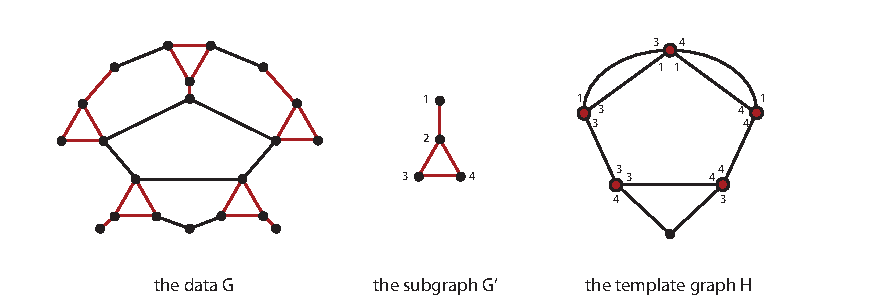
\includegraphics[width=\textwidth]{./images/illustration.pdf}
  \caption{An illustration of the motif code. We store $G'$ once, and remove its instances from $G$, replacing them with a single, special node. The links to special nodes are annotated with `rewiring' information, which tells us how to rewire the subgraph back into $H$. Storing only $H$ and $G'$ is enough to reconstruct the data.}
   \label{figure:motif-code}
\end{figure*}  

The first thing we need for this scheme is a subset $\cal M$ of ${\cal M}^\text{raw}$ such that the instances contained within it do not overlap: ie for each $M_a$ and $M_b$ in $\cal M$, we have $M_a \cap M_b = \emptyset$. Selecting the subset that would give us optimal compression is NP-Hard (as the set cover problem is reducible to it), so we must make do with an approximation. As we will see later, the most important factor is the number of links an instance has to nodes outside the instance. We call this the \emph{exdegree}.\footnote{Unlike the in- and outdegree the exdegree is not a property of a node, but of a subgraph.} In order to find a subset of instances with low exdegree, we first sort ${\cal M}^\text{raw}$ by exdegree in ascending order. We then remove the first $M$, add it to our subset $\cal M$ and remove all other instances that overlap with it. We continue removing the first remaining instance until $\cal M$ is empty.

In the following, we will often need to store a sequence of integers. We will store all such sequences using the code corresponding to a \emph{Dirichlet-Multinomial} (DM) distribution. Let $S$ be a sequence of length $k$ of elements in alphabet $\Sigma$. Conceptually, the DM distribution models the following sampling process: we sample a probability vector $p$ on $[0, |\Sigma|]$ from a Dirichlet distribution with parameter vector $\alpha$, and then sample $k$ symbols from the categorical distribution represented by $p$. The probability mass function corresponding to this process can be expressed as:
\begin{align*}
&p^\text{DirM}_\alpha(S\mid k, \Sigma) = \prod_{i \in [1,k]} \text{DirM}_\alpha(S_i\mid S_{1:i-1})  \\
&p^\text{DirM}_\alpha(S_i \mid S', k, \Sigma) = \frac{f(S_i, S') + \alpha_i}{|S'| + \sum_i \alpha_i}
\end{align*}
where $f(x, X)$ denotes the frequency of $x$ in $X$. We use $\alpha_i = 1/2$ for all $i$. Let $L^\text{DirM}_{k,\Sigma} (S) = -\log p^\text{DirM}(S \mid k, \Sigma)$. Note that this code is parametrized with $k$ and $\Sigma$. If these cannot be deduced from earlier parts of the code, they need to be encoded separately. Often, we will have $\Sigma = [0, n_\text{max}]$, and we only need to encode $n_\text{max}$.

We also require a self delimiting code to represent natural numbers. We will use the code corresponding to the probability distribution $p^\N(n) = 1/ (n(n+1))$, and denote it $L^\N(n)$.

\begin{description}
\item[subgraph] First, we store the subgraph $G'$ using $L^\text{base}(G')$ bits.
\item[template] We then create the \emph{template graph} $H$ by removing the nodes of each instance $M \in \cal M$, except for the first, which becomes a specially marked node, called an \emph{instance node}. The internal links of $M$---those incident to two nodes both in $M$---are removed from the graph. Any link connecting a node outside of $M$ to a node inside of $M$ is kept, and rewired to the instance node.
\item[instance nodes] $L^\text{base}$ does not record which nodes of $H$ are instance nodes, so we must record this separately. There are $n(G) \choose |{\cal M}|$ possibilities, so we can encode this information in $\log {n(g) \choose |{\cal M}|}$ bits.
\item[rewiring] For each side of a link in $H$ incident to an instance node, we need to know which node in the motif it originally connected to. Let there be some agreed-upon order in which to enumerate the links of any given graph. Given this order, we only need to encode the sequence $W$ of integers $w_i \in [1,\ldots, n(G')]$. We do so using the DM model described above. The maximum symbol and length of $W$ can be deduced from parts already encoded. Note that this code is invariant to the ordering of $W$, so the particulars of the canonical node ordering do not need to be specified.
\item[multiple edges] Since $L^\text{base}$ can only encode simple graphs, we cannot use it to store $H$ directly, since collapsing the instances into single nodes may have created multiple edges. In this case we remove all multiple edges and encode them separately. We assume a canonical ordering over the links and record for each link incident to an instance node, how many copies of it were removed. This gives us a sequence $R$ of natural numbers $R_i \in [0, r_\text{max}]$ which we store by first recording the maximum value in $L^\N(\max(R))$ bits, and then recording $R$ with the DM model.
\item[insertions] Finally, while $H$ and $G'$ give us enough information to recover a graph isomorphic to $G$, we cannot yet reconstruct where each node of a motif instance belongs in the node ordering of $G$. Note that the first node in the instance became the instance node, so we only need to record where to insert the rest of the nodes of the motif. This means that we perform $|{\cal M}| (n(G')-1)$ such insertions. Each insertion requires $\log (t+1)$ bits to describe, where $t$ is the size of the graph before the insertion. Let $H$ be the template graph and $G$ the complete graph, then we require $\sum_{t=n(H)}^{n(G)-1} \log (t+1) = \log (n(G)!) - \log (n(H)!)$ bits to record the correct insertions.
\end{description} 

\begin{pseudo}[th]
\caption{The motif code $L^\text{motif}(G ; G', {\cal M}, L^\text{base})$. Note that the nodes of the graph are integers.}
\label{algorithm:motif-code}
{ 
Given:\\ 
\tab a graph $G$, a subgraph $G'$,\\ 
\tab a list $\cal M$ of instances of $G'$ in $G$, a code $L^\text{base}$ on the simple graphs.\\
\\
$b_\text{subgraph} \leftarrow L^\text{base}(G')$\hfill \textbf{subgraph} \\
\\
\emph{\# replace each instance with a single node} \\
$H \leftarrow \text{copy}(G)$, $W = [] $\hfill \textbf{template} \\
\textbf{for each } $M = \{ m_1, \ldots m_{n(G')}\}$ \textbf{in} $\cal M'$:\\
\tab \emph{\# We use $m_1$ (the $m_1$-th node in $G$) as the instance node}\\
\tab \textbf{for each} link $l$ between a node $n_\text{out}$ not in $M$ and a node $m_j$ in $M$:\\
\tab \tab \textbf{if} $j \neq 1$: add a link between $n_\text{out}$ and $m_j$\\
\tab \tab $W$.append$(j)$\\
\tab remove all nodes $m_i$ except $m_1$, and all incident links\\
$b_\text{rewiring} \leftarrow  L^\text{DirM}_{|W|, n(G')}(W)\hfill\textbf{rewiring}$\\
\\
\emph{\#Remove multiple edges from $H$  and record the duplicates in $R$}\\
$R, H' \leftarrow \text{simple}(H)$ \\
$b_\text{template} \leftarrow L^\text{base}(H')$\\ 
$b_\text{multi-edges} \leftarrow L^\N(\max(R)) + L^\text{DirM}_{|R|, \max(R)}(R)$ \hfill \textbf{multiple edges}\\
\\
$b_\text{instances} \leftarrow \log {n(G) \choose |{\cal M'}|}$ \hfill \textbf{instance nodes}\\
$b_\text{insertions} \leftarrow \log (n(G))! - \log (n(H))!$ \hfill \textbf{insertions}\\    
\\
\textbf{return} $b_\text{subgraph} + b_\text{template} + b_\text{rewiring} + b_\text{multi-edges} + b_\text{instances} + b_\text{insertions}$\\
}
\end{pseudo} 

\paragraph{search} Since our code accepts any list of motif instances, we are free to take the list $\cal M$ and prune it further, before passing it to the motif compressor, effectively discounting instances of the motif. This can often improve compression, as storing the rewiring information for instances with high exdegrees may cost more than we gain from removing them from the graph. We will sort  $\cal M$ by exdegree and search for the value $c$ for which compressing the graph with only the first $c$ elements of $\cal M$ gives the lowest codelength.

The codelength $L^\text{motif}$ as a function of $c$ is roughly unimodal, which means that a ternary search should give us a good value of $c$ while reducing the number of times we have to compute the full codelength. We use a \emph{Fibonacci search} \cite{kiefer1953sequential}, an elegant variation on ternary search requiring only one sample per recursion. Note that $c$ is not a parameter of the model, so we do not need to store it separately.  

\paragraph{implementation} The \textbf{template} part of the code can be time and memory intensive for large graphs, as it involves creating a copy of the data. For any given $L^\text{base}$, we can create a specific implementation which computes the codelength required for storing the template graph without constructing $H$ explicitly. This will speed up the computation of the code at the expense of creating a new implementation for each new null model. We use such specific implementations for our three null models.

\section*{Null Models}

We will define three null models. For each model we follow the same pattern, we first describe a parametrized model (which does not represent a code on all graphs). We then use this to derive a bound as described in the second section, so that we can reject a set of null models, and finally we describe how to turn the parametrized model into a complete model to store graphs within the motif code.  

Specifically, let $L^\text{name}_\theta(G)$ be a parametrized model with parameter $\theta$. Let $\hat\theta(G)$ be the value of $\theta$ that minimizes $L^\text{name}_\theta(G)$ (the maximum likelihood parameter). From this we derive a bound $B^\text{name}(G)$ from this---usually using $B^\text{name}(G) = L^\text{name}_{\hat\theta(G)}(G)$---which we will use in place of a null-model. Finally, we create the complete model by two-part coding: $L^\text{name}(G) = L^{\theta}(\hat\theta(G)) + L^\text{name}_{\hat\theta(G)}(G)$. 

\subsection*{The Erd\H{o}s-Renyi Model}

The Erd\H{o}s-Renyi (ER) model is probably the best known probability distribution on graphs\cite{renyi1959random,gilbert1959random}. It takes a number of nodes $n$ and a number of links $m$ as parameters, and assigns equal probability to all graphs with these attributes, and zero probability to all others. This gives us 
\[
L^\text{ER}_{n, m}(G) = \log{(n^2-n)/2 \choose m} 
\] 
for undirected graphs, and 
\[
L^\text{ER}_{n, m}(G) = \log{n^2-n \choose m} 
\] 
for directed graphs. We use the bound $B^\text{ER}(G) = L^\text{ER}_{n(G), m(G)}(G)$.

For a complete code on simple graphs, we encode $n$ with $L^\N$. For $m$ we know that the value is at most $m_\text{max}=(n^2-n)/2$ in the undirected case, and at most $m_\text{max}=n^2-n$ in the directed case, and we can encode such a value in $\log m_\text{max}$ bits: 
\[
L^\text{ER}(G) = L^\N(n(G)) + \log m_\text{max} + L^\text{ER}_{n(G), m(G)}(G)\p
\]
 
\subsection*{The Degree-Sequence Model}
\label{section:degree-sequence-model}

The most common null-model in motif analysis is the \emph{degree-sequence model} (also known as the \emph{configuration model} \cite{newman2010networks}). 
For undirected graphs, we define the degree sequence of graph $G$ as the sequence $D(G)$ of length $n(G)$ such that $D_i$ is the number of links incident to node node $i$ in $G$. For directed graphs, the degree sequence is a pair of such sequences $D(G) = (D^\text{in}, D^\text{out})$, such that $D^\text{in}_i$ is the number of incoming links of node $i$, and $D^\text{out}_i$ is the number of outgoing links.

\paragraph{The parametrized model $L^\textnormal{DS}_D(G)$} The degree-sequence model $L^\text{DS}_D(G)$ takes a degree sequence $D$ as a parameter and assigns equal probability to all graphs with that degree sequence. Assuming that $G$ matches the degree sequence, we have $L^\text{DS}_D(G) = \log |\cG_D|$ where $\cG_D$ is the set of simple graphs with degree sequence $D$. There is no known efficient way to compute this value for either directed or undirected graphs, but various estimation procedures are known. We use an importance sampling algorithm discovered independently by \cite{blitzstein2011sequential} and \cite{charo2010efficient}.\footnotemark~This algorithm is guaranteed to produce any graph matching $D$ with some nonzero probability. Crucially, the algorithm does not backtrack or reject candidates, which means that if we multiply the probability of each random choice made in sampling, we get the probability of the sample under our sampling procedure. That is, the algorithm produces, along with a sample $G \in \cG_D$, the probability $q^\text{DS}_D(G)$ of the algorithm producing $G$. While the samples are not uniform, we do have:
\begin{equation}
{E} \left [\frac{1}{q^\text{DS}_D(G)}\right] = |\cG_D| \label{line:expectation}
\end{equation}
where $G$ is a random variable representing a sample from the algorithm. Thus, we can sample a number of graphs and take the mean of their inverse probability under $q^\text{DS}_D$ to estimate $p^\text{DS}_D(G)$. This is a form of \emph{importance sampling}. 

This approach was taken in \cite{blitzstein2011sequential}: the sample mean $1/n \sum_i 1/q^\text{DS}_D(G_i)$ was used as an estimator for the expectation in (\ref{line:expectation}). However, as shown in \cite{charo2010efficient}, the distribution of $1/q^\text{DS}_D(G)$ tends to be very close to log-normal. This means that the sample mean will converge \emph{very} slowly to the correct value. Specifically, the standard deviation of this estimate after $n$ samples is $\frac{1}{\sqrt{n}} \sqrt{(e^{\sigma^2}-1)e^{2\mu +\sigma^2}}$, which for a distribution with $\mu=200$ and $\sigma=10$, leads to a standard deviation of approximately $\frac{1}{\sqrt{n}} e^{300}$.

For this reason, we use the \emph{maximum-likelihood estimator} for the log-normal distribution instead. Let $Q_i = 1/q^\text{DS}_{D}(G_i)$. We assume $Q_i$ is log-normally distributed, so that $Y_i = \log Q_i$ is normally distributed. Let $\overline{Y} = \frac{1}{n}\sum_i Y_i$ and $S_Y = 1/n \sum_i (\overline{Y} - Y_i)^2$; then the maximum-likelihood estimator of $EQ$ is $\exp\left(\overline{Y} + \frac{1}{2}S_Y\right)$. Thus, the codelength under the degree sequence model can be estimated as $\left(\overline{Y} + \frac{1}{2}S_Y\right)\log_2(e)$.

\footnotetext{Specifically, our implementation uses the algorithms described in \cite{charo2010efficient} and \cite{kim2012constructing}. However the non-uniform sampling from the candidate set, discussed in \cite[p10, step 5]{blitzstein2011sequential} is crucial to achieving a low variance in the sampling distribution, and thus a fast convergence.}

Unfortunately, even with the highly optimized implementations described in \cite{charo2010efficient} and \cite{kim2012constructing} sampling can be slow for large graphs. Luckily, we are only interested in an estimate of the codelength accurate to around the level of single bits, which means that we only need to sample until we have a rough estimate of the order of magnitude of $|\cG_D|$. For instance, if we accept a margin of error of only 15 bits (of the potentially $10^6$ bits required to store the graph), we can underestimate the number of graphs by 4 orders of magnitude and still end up within the margin. All we need is a reliable confidence interval for our estimate, so that we can choose a suitably conservative bound for our estimate. Our method of obtaining such a confidence interval is described in the supporting materials. In all cases, we use a one-sided confidence interval: when computing the codelength under the null model, we use a lower bound for the true value, and when computing the codelength for the motif code, we use an upper bound. Thus, the difference in codelength is a lower bound for the true value.

\paragraph{The bound $B^\textnormal{DS}(G)$} To get a bound for all two-part codes on $L^\text{DS}_D$, we could use ${B'}^\text{DS}(G) = L^\text{DS}_{D(G)}(G)$. Beating such a bound would tell us that no property of the degree sequence could explain the motif we had found. Unfortunately, the degree sequence forms a large part of the code, and a lot of evidence is required to compress better than ${B'}^\text{DS}(G)$ with a complete code. 

Instead, we make the assumption that the degrees are sampled independently from a single distribution $p^\text{deg}(n)$ on the the natural numbers. This corresponds to a code $\sum_{D_i \in D}L^\text{deg}(D_i)$ on the entire degree sequence. Let $f(s, D)$ be the frequency of symbol $s$ in sequence $D$. It can be shown that $B^\text{deg}(D) = \sum_{D_i \in D} f(D_i, D)/|D|$ is a lower bound for any such code on the degree sequence. This gives us the bound $B^\text{DS}(G) = B^\text{deg}(D(G))) + L^\text{DS}_{D(G)}(G)$. For directed graphs, we use $B^\text{DS}(G) = B^\text{deg}(D^\text{in}(G))) + B^\text{deg}(D^\text{out}(G))) + L^\text{DS}_{D(G)}(G)$

\paragraph{The complete model $L^\textnormal{DS}(G)$} For the alternative model we need a complete code. First, we store $n(G)$ with $L^\N$. We then store the maximum degree and encode the degree sequence with the DM model. For undirected graphs we get: 
\[
L^\text{DS}(G) = L^\N(n(G)) + L^\N(\max(D)) + L^\text{DirM}_{n(G), \max(D)}(D) + L^\text{DS}_{D(G)}(G)
\]
and for directed graphs
\begin{align*}
L^\text{DS}(G) = &L^\N(n(G)) \\ 
 + &L^\N(\max(D^\text{in})) + L^\text{DirM}_{n(G), \max(D^\text{in})}(D^\text{in})\\
 + &L^\N(\max(D^\text{out})) + L^\text{DirM}_{n(G), \max(D^\text{out})}(D^\text{out}) + L^\text{DS}_{D(G)}(G) \p
\end{align*} 

Note that in the computation of $L^\text{motif}$ with $L^\text{DS}$ as a base model, we estimate $|\cG_D|$ for both the template graph and the motif. It is important to combine the confidence intervals over these two estimates carefully, so that we end up with a correct confidence interval over the total codelength. This is discussed in the supporting materials. For $L^\text{motif}$, we compute a one-sided confidence interval to get an \emph{upper}bound, so that with 95\% confidence we are \emph{over}estimating the size of the motif code. 

\subsection*{The Edgelist Model}

While estimating $|\cG_D|$ can be costly, we can compute an upper bound efficiently. Assume that we have a directed graph $G$ with $n$ nodes, $m$ links and a pair of degree sequences $D = (D^\text{in}, D^\text{out})$. To describe $G$, we might write down the links as a pair of sequences $(F, T)$ of nodes: with  $F_i$ the node from which link $i$ originates, and $T_i$ the node to which it points. Let $S_d$ be the set of all pairs of such sequences satisfying $D$. We have $ m \choose D_1^\text{in}, \ldots, D_n^\text{in}$ possibilities for the first sequence, and $m \choose D_1^\text{out}, \ldots, D_n^\text{out}$ for the second. This gives us $|S_D| = {m \choose D_1^\text{in}, \ldots, D_n^\text{in}}{m \choose D_1^\text{out}, \ldots, D_n^\text{out}} = m!m! / \prod_{i=1}^n D^\text{in}_i ! D^\text{out}_i !$. We have $|S_D| > |\cG_D|$ for two reasons. First, many of the graphs represented by such a sequence pair contain multiple links and self-loops, which means they are not in $\cG_D$. Second, the link order is arbitrary: we can interchange any two different links, and we would get a different pair of sequences, representing the same graph, so that for a graph with no multiple edges, there are $m!$ different sequence-pairs to represent them. 

To refine this upper bound, let $S'_D \subset S_D$ be the set of sequence pairs representing simple graphs. Since all links in such graphs are distinct, we have $|\cG_D| = |S'_D|/m!$. Since $|S'_D| \leq |S_D|$, we have \footnotemark
\[
|\cG_D| \leq \frac{m!}{\prod_{i=1}^n D^\text{in}_i ! D^\text{out}_i !} \p
\]

\footnotetext{This value was previously used in \cite{bezakova2006graph} as a precise value for the number of graphs with multiple edges. This is incorrect, as we can only divide by $m!$ if we know that no graphs have multiple edges.}

In the undirected case, we can imagine a single, long list of nodes of length $2m$. We construct a graph from this by connecting the node at index $i$ in this list to the node at index $m+i$ for all $i \in [1, m]$. In this list, node $a$ should occur $D_a$ times. We define $S_D$ as the set of all lists such that the resulting graph satisfies $D$. There are $(2m)! \choose D_1, \ldots, D_n$ such lists.
We now have an additional reason why $|S_D| > |\cG_D|$: each pair of nodes describing a link can be swapped around to give us the exact same graph. This gives us:
\[
|\cG_D| \leq |S'_D| / (2^m m!) = \frac{(2m)!}{2^m m! \prod_{i=1}^n D_i!} \p
\]

In both cases, the fact that we have an upperbound gives us a code: while the code as described assigns some probability mass to non-simple graphs, we can easily assume that this is assigned instead to some null-element, since we are only interested in the codelengths and probabilites of simple graphs. This gives us the following parametrized code for directed graphs:
\[
L^\text{EL}_D(G) = \log m! - \sum_{i=0}^n \log D_i^\text{in}! - \sum_{i=0}^n \log D_i^\text{out}!   
\]
where $(D^\text{in}, D^\text{out})$ are the degree sequences of $G$, and for the undirected case:
\[
L^\text{EL}_D(G) = \log (2m)! - \log m! - m - \sum_{i=0}^n \log D_i! \p   
\]

For the bound and the complete model, we follow the same strategy we used for the degree-sequence model: $B^\text{EL}(G) = B^\text{deg}(G) + L^\text{EL}_{D(G)}(G)$ and, 
\[
L^\text{EL}(G) = L^\N(n(G)) + L^\N(\max(D)) + L^\text{DirM}_{n(G), \max(D)}(D) + L^\text{EL}_{D(G)}(G)
\] for undirected graphs and 
\begin{align*}
L^\text{EL}(G) = &L^\N(n(G)) \\ 
 + &L^\N(\max(D^\text{in})) + L^\text{DirM}_{n(G), \max(D^\text{in})}(D^\text{in})\\
 + &L^\N(\max(D^\text{out})) + L^\text{DirM}_{n(G), \max(D^\text{out})}(D^\text{out}) + L^\text{EL}_{D(G)}(G)
\end{align*} for directed graphs.

\section*{Experiments}

To validate and illustrate our method, we will perform three experiments. First, we will construct a graph by injecting instances of a single motif into a random network. The method should recover only this motif as significant. Second, we will run the method on datasets from four different domains, and show the results for the most frequent subgraphs, using the three null-models we have described. Finally, to show the scalability of the model with fast null models, we will run the analysis on a large graph.

In all experiments we search for motifs by sampling, based on the method described in \cite{kashtan2004efficient}. Note that we have no particular need for a sampling algorithm which provides an accurate approximation of the actual frequencies present in the graph, so long as it can provide us with a large selection of non-overlapping instances with low exdegree. For this reason we adapt the algorithm to improve its speed: we start with an empty selection of nodes $N'$, and add a random node drawn uniformly. We then add to $N'$ a random neighbour of a random member of $N_G$, and repeat this action until $N'$ has the required size. We then extract and return $I(N', G)$. In the case of a directed graph, nodes reachable by incoming and outgoing links are both considered neighbours.  

The size $n(G')$ of the subgraph is chosen before each sample from a uniform distribution over the interval $[n_\text{min}, n_\text{max}]$.

We re-order the nodes of the extracted graph to a canonical ordering for its isomorphism class, using the Nauty algorithm \cite{mckay1981practical}. We maintain a map from each  subgraph in canonical form to a list of instances found for the subgraph. After sampling is completed, we end up with a set of potential motifs and a list of instances for each, to pass to the motif code described in the Section \emph{Encoding with Motifs}.

In all experiments we report the log-factor: $B^\text{null}(G) - L^\text{motif}(G; G', {\cal M}, L^\text{null})$. That is we use the bound in place of the null model, and the complete code of the same null model is passed to the motif code. If the log-factor is larger than 10 bits, we can interpret it, as described in the section \emph{Model Selection by Codelength}, as a successful significance test, allowing us to reject the null model at $\alpha=0.001$. In all cases, a negative log-factor means that we do not have sufficient evidence to reject the null-model, but a different experiment might yet achieve a positive log-factor. This could be achieved by sampling more subgraphs, using a different algorithm to find motif instances or taking more samples from the degree-sequence estimator.

\subsection*{Recovering Motifs in Synthetic Data}

\label{section:recovering}

We use the following procedure to sample an undirected graph with $5000$ nodes and $10000$ links, containing $n^i$ injected instances of a particular motif $G'$ with $n'$ nodes and $m'$ links:

\begin{enumerate}
  \item Let $n = 5000 - (n'-1)n^i$ and $m = 10000 - m'n^i$ and sample a graph $H$ from the uniform distribution over all graphs with $n$ nodes and $m$ links.   
  \item Label $n^i$ random nodes, with degree 5 or less, as instance nodes.
  \item Let $p^\text{cat}$ be a categorical distribution on $\{1, \ldots, 5\}$, chosen randomly from the uniform distribution over all such distributions.
  \item Label every connection between an instance node and a link with a random value from $p^\text{cat}$. Links incident to two instance nodes, will thus get \emph{two} values.
  \item Reconstruct the graph $G$ from $G'$ and $H$.
\end{enumerate}

This is roughly similar to sampling from our motif code. In this graph, $G'$ should be the only significant motif, with the exception of motifs that can be explained from the prevalence of $G'$, ie. subgraphs and supergraphs of $G'$, or graphs that contain part of $G'$. However, these should have a markedly lower log-factor than $G'$. For our experiment, we will only extract subgraphs of size 5, to rule out the first two cases.

On this sampled graph, we run our motif analysis. We run the experiment multiple times, with $n^i = 0$, $n^i = 10$ and $n^i = 100$, using the same subgraph $G'$ over all runs, but sampling a different $H$ each time. For each value of $n^i$, we repeat the experiment 10 times. Per run we sample 5000 motifs. This value is chosen to show that even a very \emph{low} sample size is sufficient to recover the motif. The null-model in all cases is the ER model, as that corresponds to the source of the data.

Fig.~\ref{figure:plot-synthetic} shows the results for the 21 possible connected simple graphs of size 5. As expected, when we insert no subgraphs, the motif model cannot compress the graph better than the null model, for any motifs, since the source of the data \emph{is} the null-model. There are motifs with very high frequencies (shown on the right), much higher than the frequencies of our motif, but these can be explained as a consequence of the null model and have a negative log-factor. We can also see that once we insert 100 instances of the motif, two other subgraphs become motifs: in both cases, these share a part of the inserted motif (a rectangle and a triangle). This is an important lesson for motif analysis: not every motif represents a meaningful result, some motifs may be a byproduct of other motifs. 

\begin{figure*}[htb]
  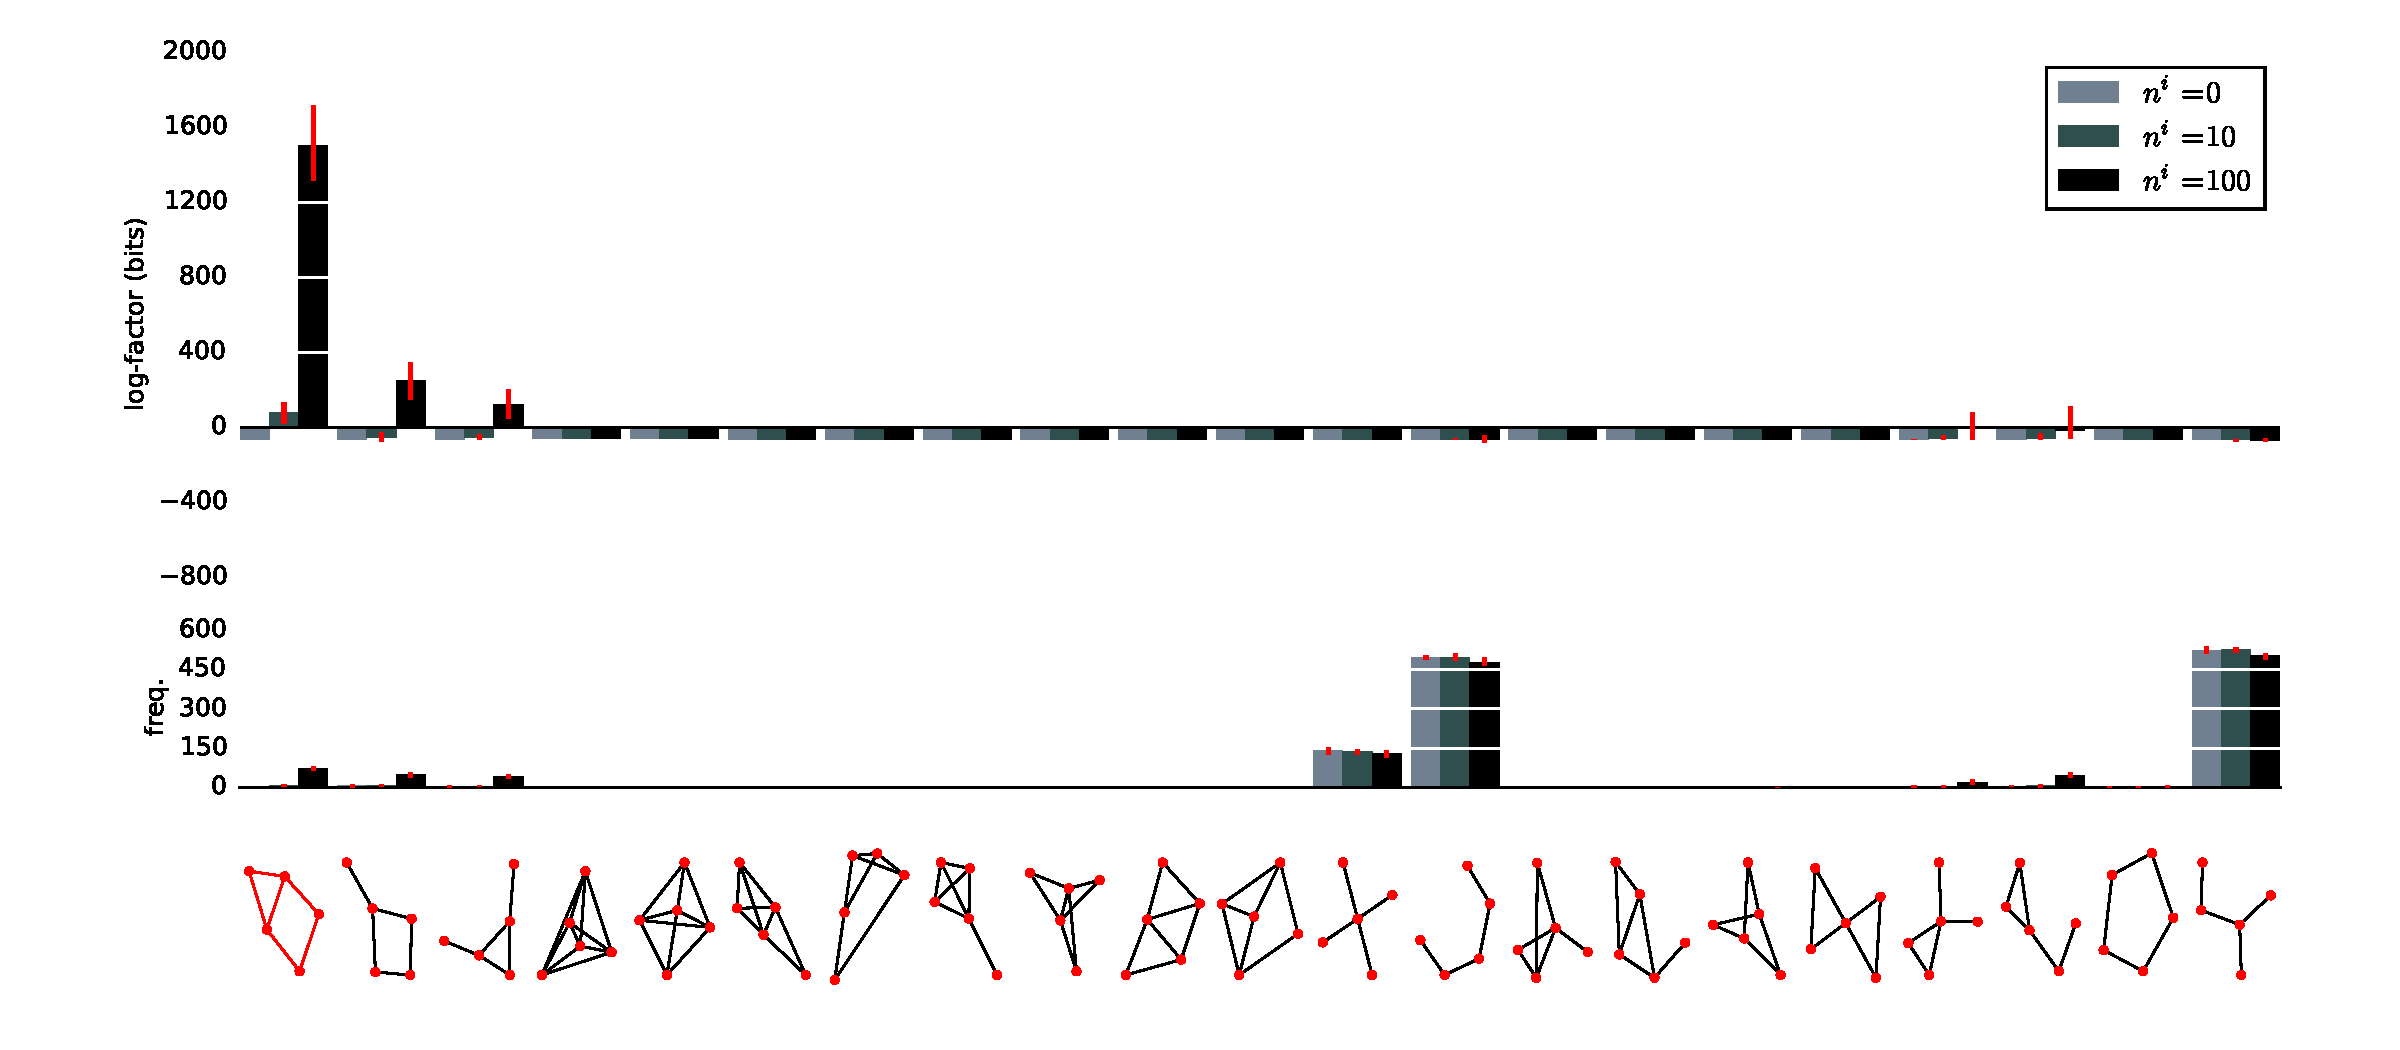
\includegraphics[width=\textwidth]{./images/synthetic-plot.pdf}
  \caption{\small The results of the experiment on synthetic data. The bottom row shows all 21 simple connected graphs with 5 nodes (up to isomorphism). The middle row shows the number of non-overlapping instances found by the sampling algorithm for $n^i = 0$, $n^i=10$ and $n^i=100$ from left to right, for each motif. The bars show the average value over 10 randomly sampled graphs, with the same subgraph (shown in red) injected each time. The top row shows the difference between  the code length under the null model (the ER model) and under the motif code. The error bars represent the \emph{range}, ie. they are drawn from the smallest to the largest observation.}
  \label{figure:plot-synthetic}
\end{figure*}

\subsection*{Various Datasets and Null-Models}
\label{section:various}

Next, we show how our our approach operates on a selection of datasets across domains. We use the following datasets:
\begin{description}

\item[kingjames (undirected, $n=1773, m=9131$)] Co-occurrences of nouns in the text of the King James bible \cite{konect:2014:moreno_names,konect:harrison}. Nodes represent nouns (places and names) and links represent whether these occur together in one or more verses.
\item[yeast (undirected, $n=1528, m=2844$)] A network of the protein interactions in yeast, based on a literature review \cite{reguly2006comprehensive}. Nodes are proteins, and links are reported interactions between proteins. We removed 81 self-loops.
\item[physicians (directed, $n=241, m=1098$)] Nodes are physicians in Illinois \cite{konect:2015:moreno_innovation,konect:coleman1957}. Links indicate that one physician turns to the other for advice.
\item[citations (directed, $n=1769, m=4222$)] The arXiv citation network in the category of theoretical astrophysics, as created for the 2003 KDD Cup \cite{gehrke2003overview}. To create a workable graph, we follow the procedure outlined in \cite{carstens2013motifs}: we include only papers published before 1994, remove citations to papers published after the citing paper, and select the largest connected component.
\end{description}

All datasets are simple (no multiple edges, no self-loops). In each case we take $5 \cdot 10^6$ samples with $n_\text{min} = 2$ and $n_\text{max} = 6$. We test the 100 motifs with the highest number of instances (after overlap removal), and report the log-factor for each null model. For the edgelist and ER models we use a Fibonacci search at full depth, for the degree-sequence model we restrict the search depth to $3$. For the degree-sequence estimator, we use $40$ samples and $\alpha=0.05$ to determine our confidence interval. We use the same set of instances for each null-model.

\begin{figure*}[h]
  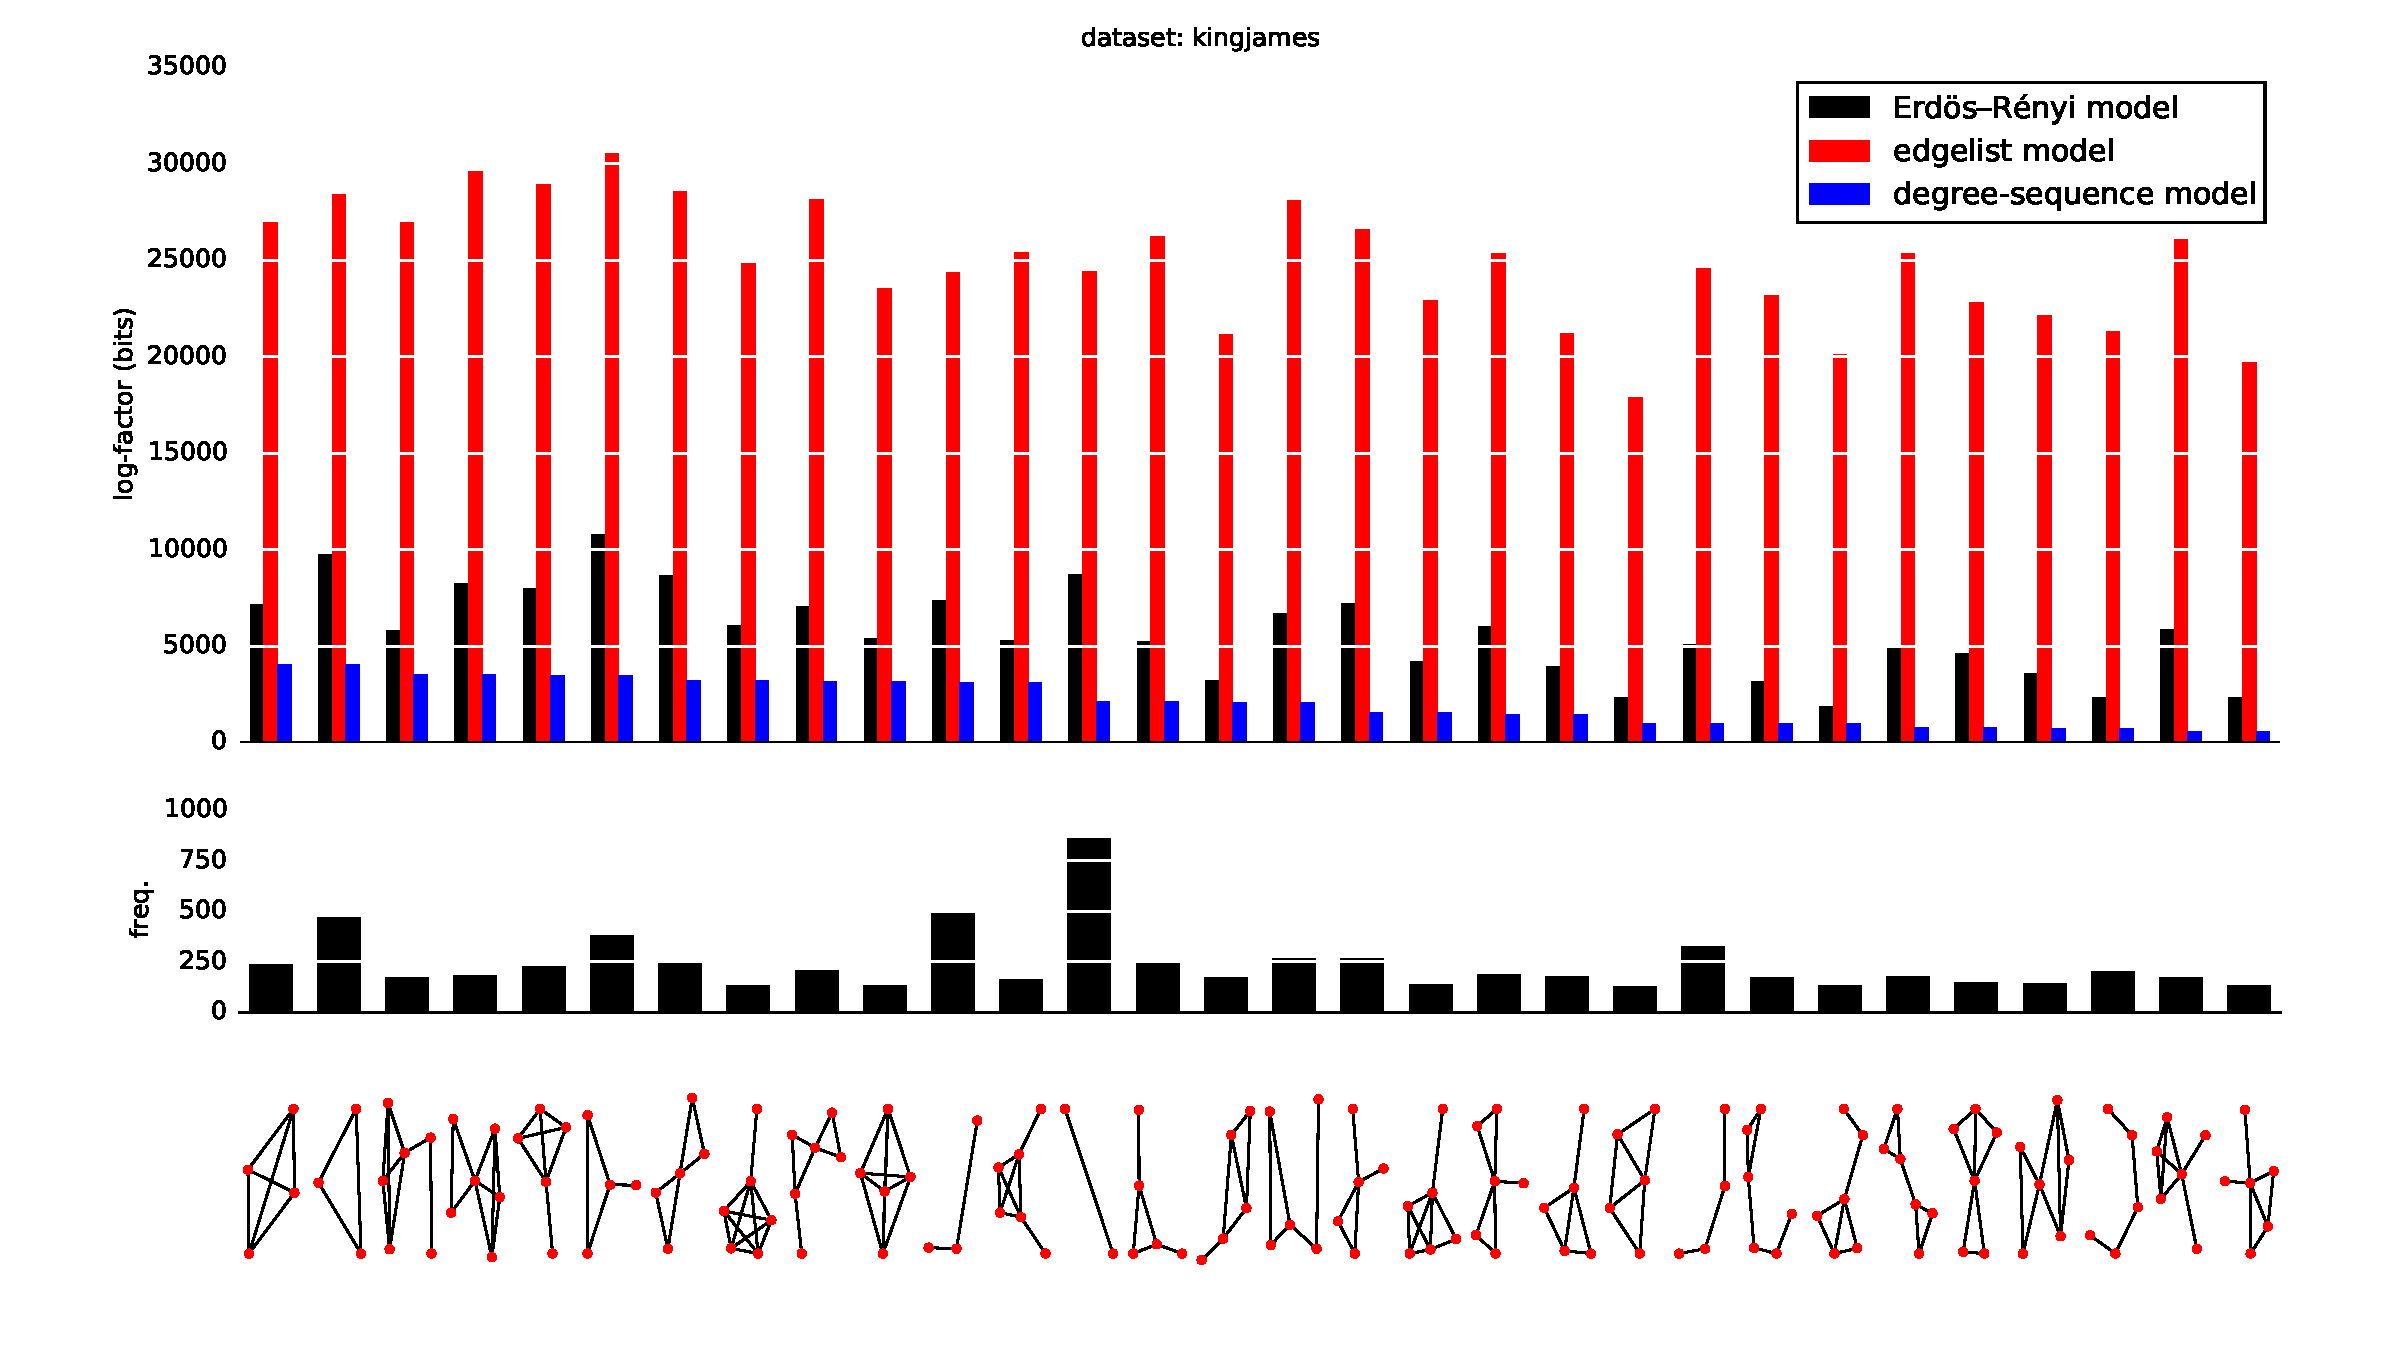
\includegraphics[width=\textwidth]{./images/kingjames/compare-plot.pdf}\\
  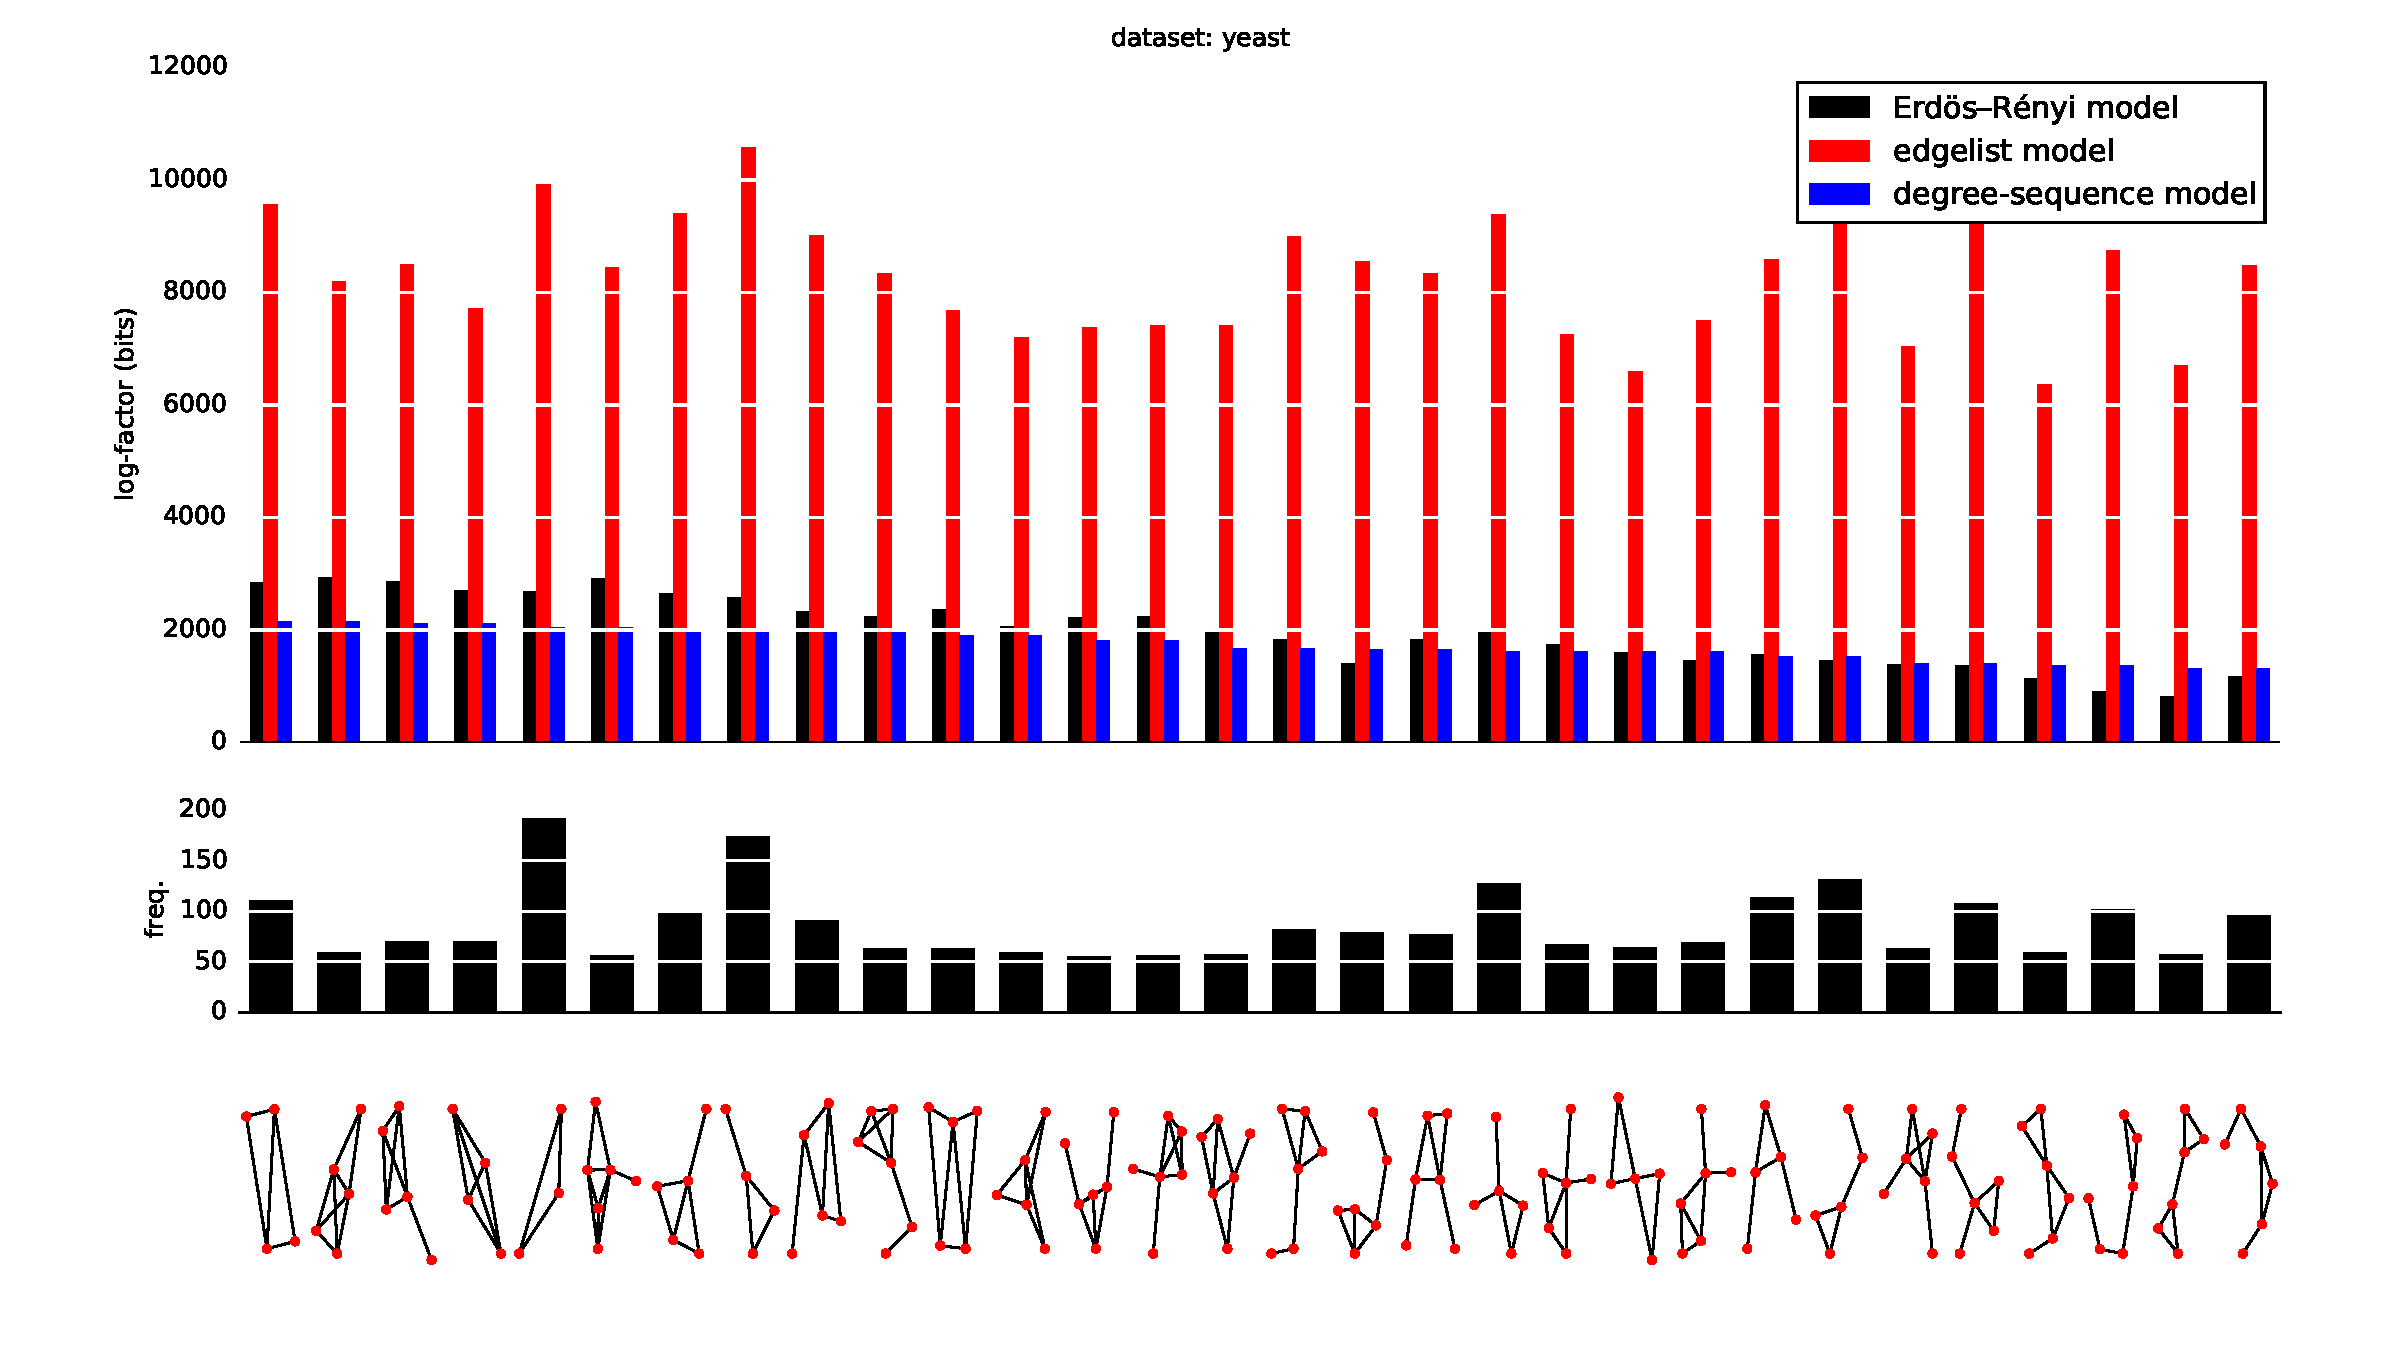
\includegraphics[width=\textwidth]{./images/yeast/compare-plot.pdf}\\
  \caption{The results of the motif extraction on the 2 undirected networks.}
  \label{figure:plot-und}
\end{figure*}
  
\begin{figure*}[h]
  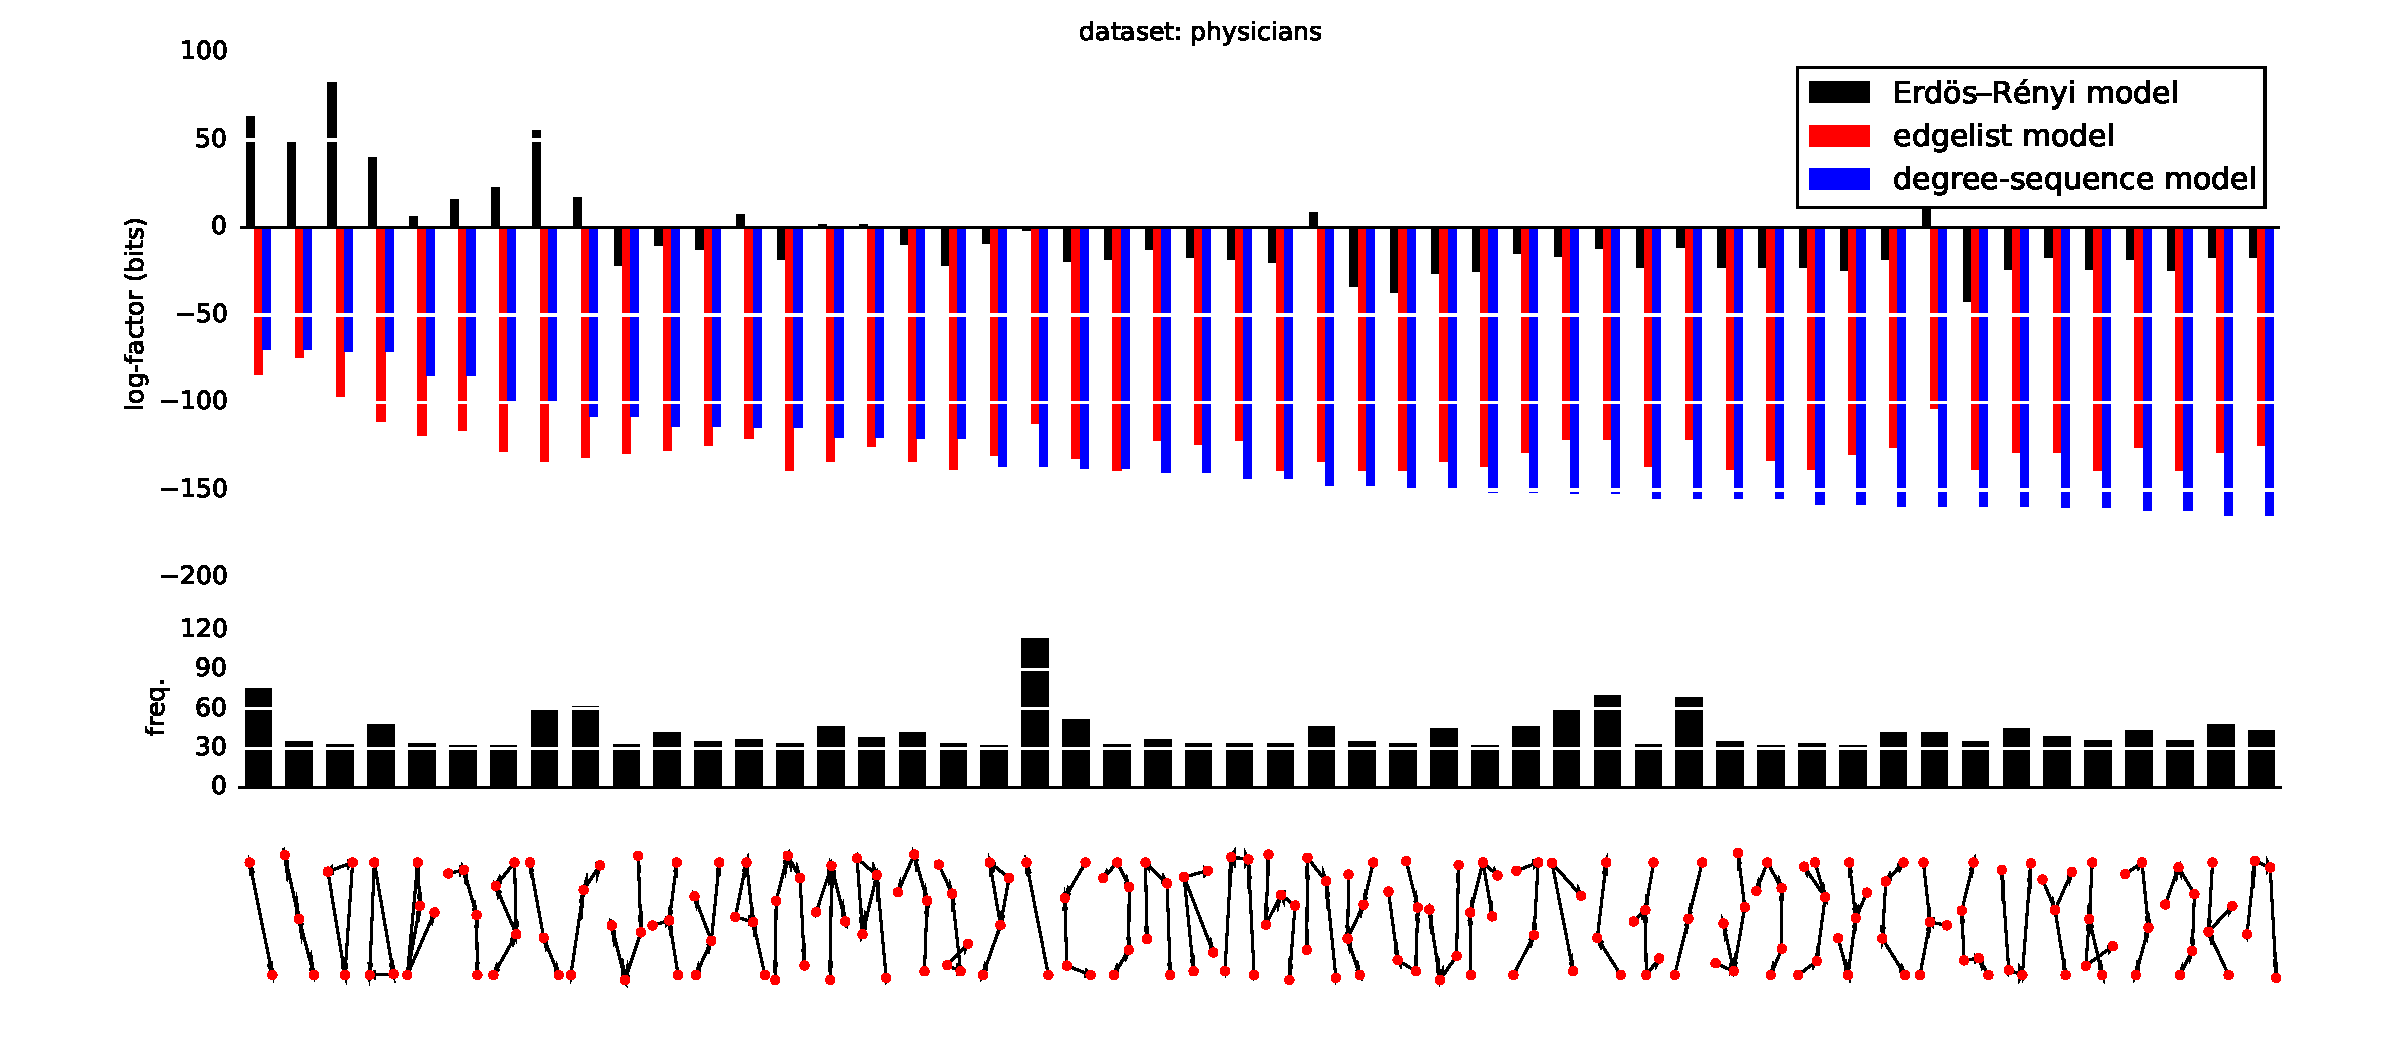
\includegraphics[width=\textwidth]{./images/physicians/compare-plot.pdf}\\
  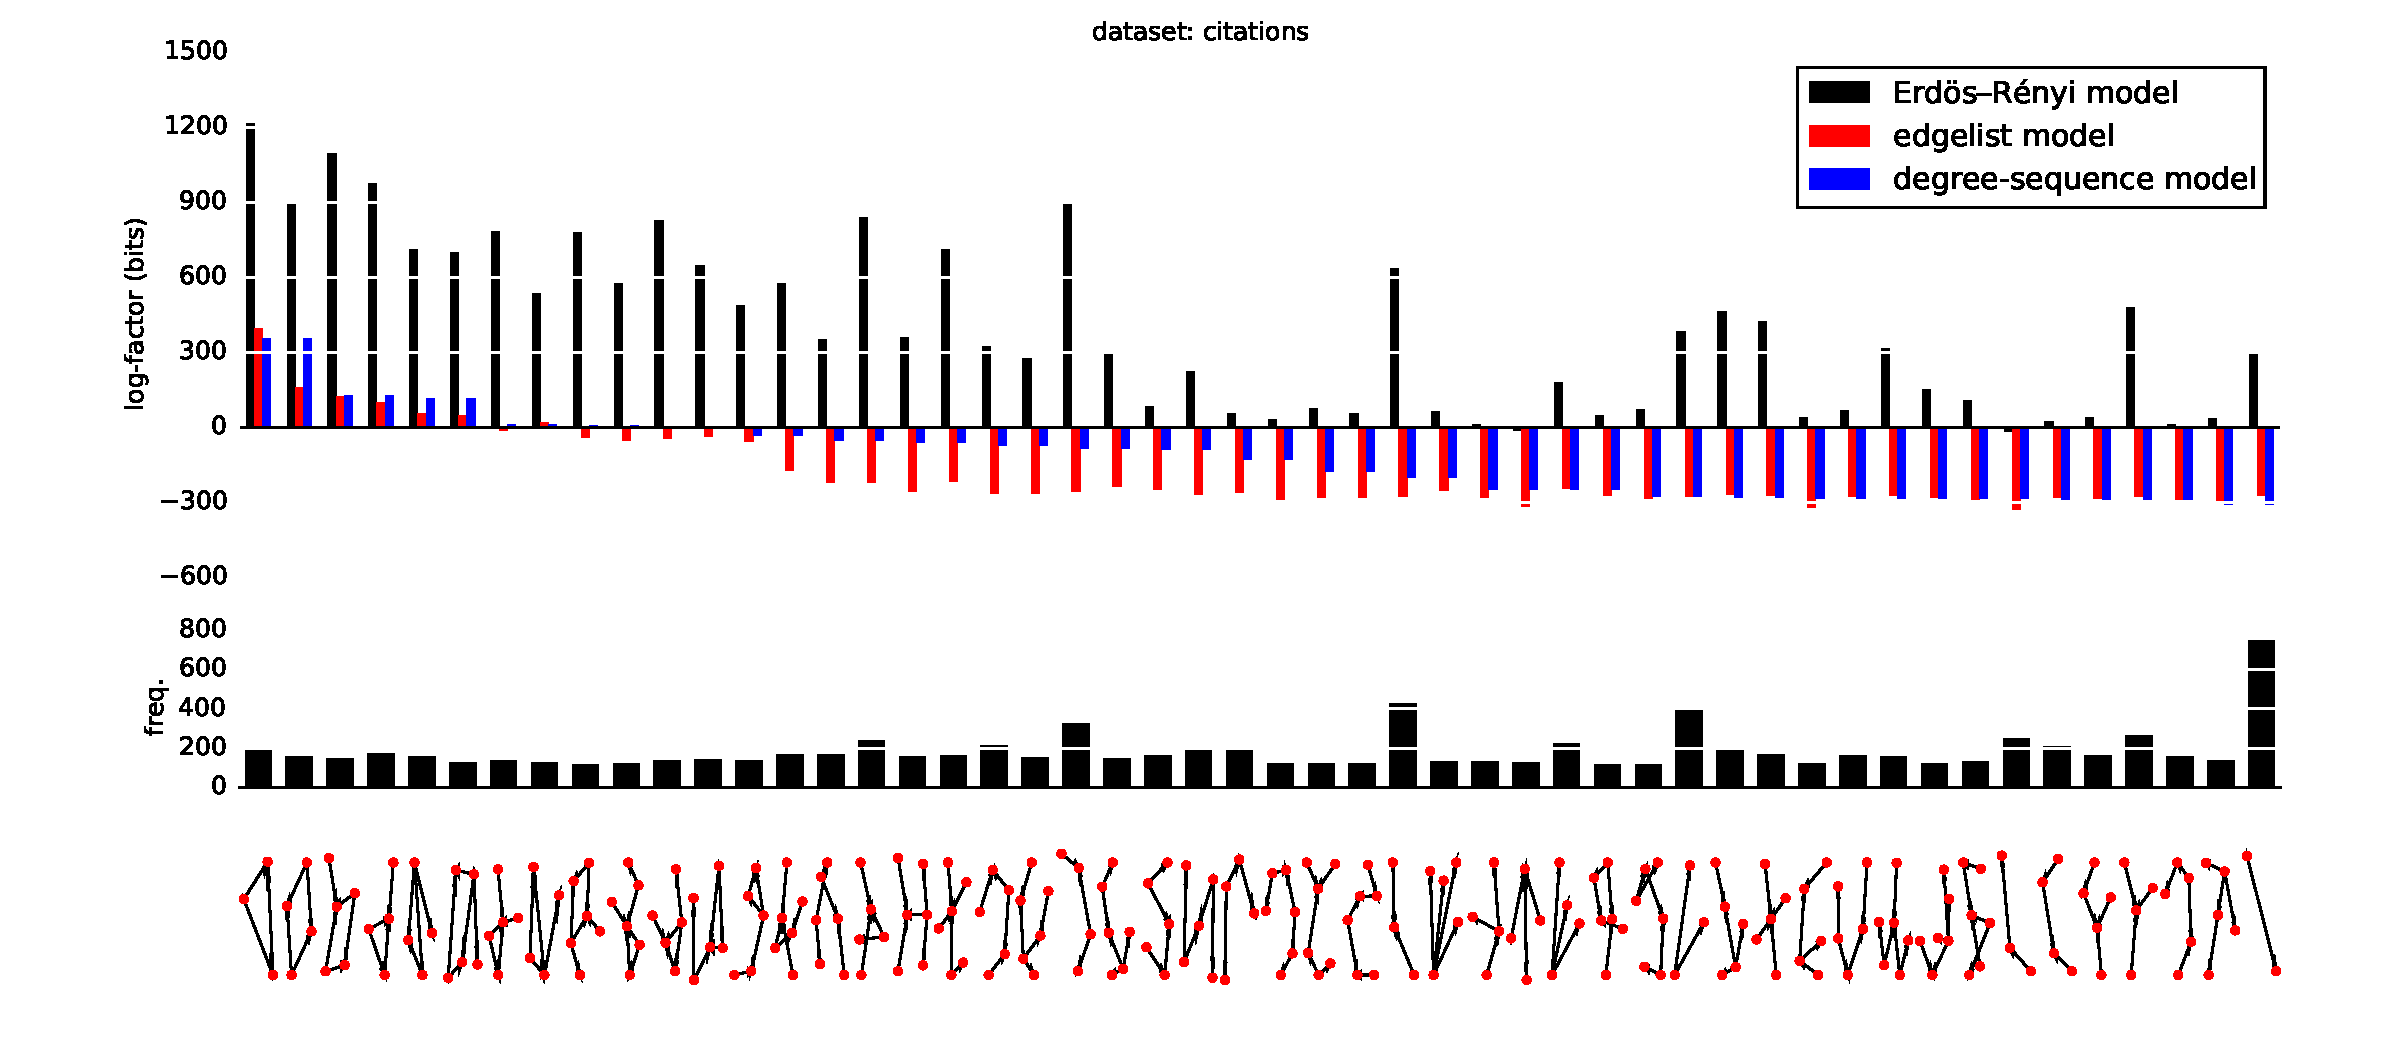
\includegraphics[width=\textwidth]{./images/citations/compare-plot.pdf}\\
  \caption{The results of the motif extraction on the 2 directed networks.}
  \label{figure:plot-dir}
\end{figure*}

Our first observation is that for the physician dataset, there are no motifs under the degree-sequence null-model. We have found this to be a common property of many social networks. Whether this indicates that social networks are simpler, more random, or perhaps even well-modeled by the degree sequence model, requires further investigation. We may be tempted to draw the conclusion that directed networks contain fewer motifs for these null models, or that fewer motifs can be found in directed networks with this method, but the experiment in the next section shows that that is not the case. 

In both the kingjames and the yeast graphs, many motifs contain cliques or near-cliques. This suggests that the data contains local communities of highly connected nodes which the null model cannot explain.

We also observe a degree of agreement between the degree sequence model and the edgelist model, suggesting that the edgelist model may be an acceptable proxy for the degree sequence model.

These analyses were run on a single machine with 8 Gigabyte of java heapspace \footnote{This was the system default. The amount of memory used was not measured.} and 2 1.80 Ghz Intel Xeon processors (E5-2650L). For the kingjames dataset the time taken was, on average, 23 minutes and 34 seconds per motif. For the yeast dataset, 3 minutes and 8 seconds per motif. For the physicians dataset, 35 seconds per motif and for the citations dataset 9 minutes and 25 seconds per motif. In all these experiments the degree-sequence model took by far the most time. The next section shows the possibilities if this model is not considered.
 
The sampling from the degree-sequence estimator was done in parallel, taking advantage of the 16 cores available in total. All other code was single-threaded. 

\subsection*{Large-Scale Motif Extraction}
\label{section:large}

In the experiments above, the computation of $L^\text{DS}_D$ was by far the greatest bottleneck. In order to test the scalability of the method for null-models which can be computed efficiently, we omit the degree-sequence null model. This allows us to perform motif detection on much larger graphs. We use the hyperlink graph of the Dutch Wikipedia \cite{konect:2015:link-dynamic-nlwiki,konect:unlink} as a benchmark. This dataset contains all links that existed at some point between any two articles of the Dutch Wikipedia. We removed self loops and multiple edges, resulting in a network of 1 039 253 nodes and 13 485 902 links.  We sampled $5 \cdot 10^6$ subgraphs of sizes from 2 to 6 nodes. We selected the 100 motifs with the greatest number of instances (after overlap removal) and computed their log-factor under the ER and edgelist models. The top 30 are shown in Fig.~\ref{figure:plot-large}. We used the Fibonacci search at full depth for both models.

The analysis was executed using 3.5 gigabytes of Java heapspace, on a machine with 2 1.80 Ghz Intel Xeon processors (E5-2650L). It took 5 hours and 27 minutes to complete. Sampling of subgraphs took 9 minutes, overlap removal took 14 minutes and the compression analysis took, on average, 3 minutes and 2 seconds per motif (for 100 motifs analyzed).

Note that all code in this analysis is single-threaded, so the availability of multiple cores and multiple processors was \emph{not} exploited. While it is a simple matter to run the computation of the log-factors in parallel, with a thread for each motif, a single-threaded run shows that the experiment can also be run on commodity hardware, in reasonable time.

\begin{figure*}[htb]
  \hspace{-4cm}
  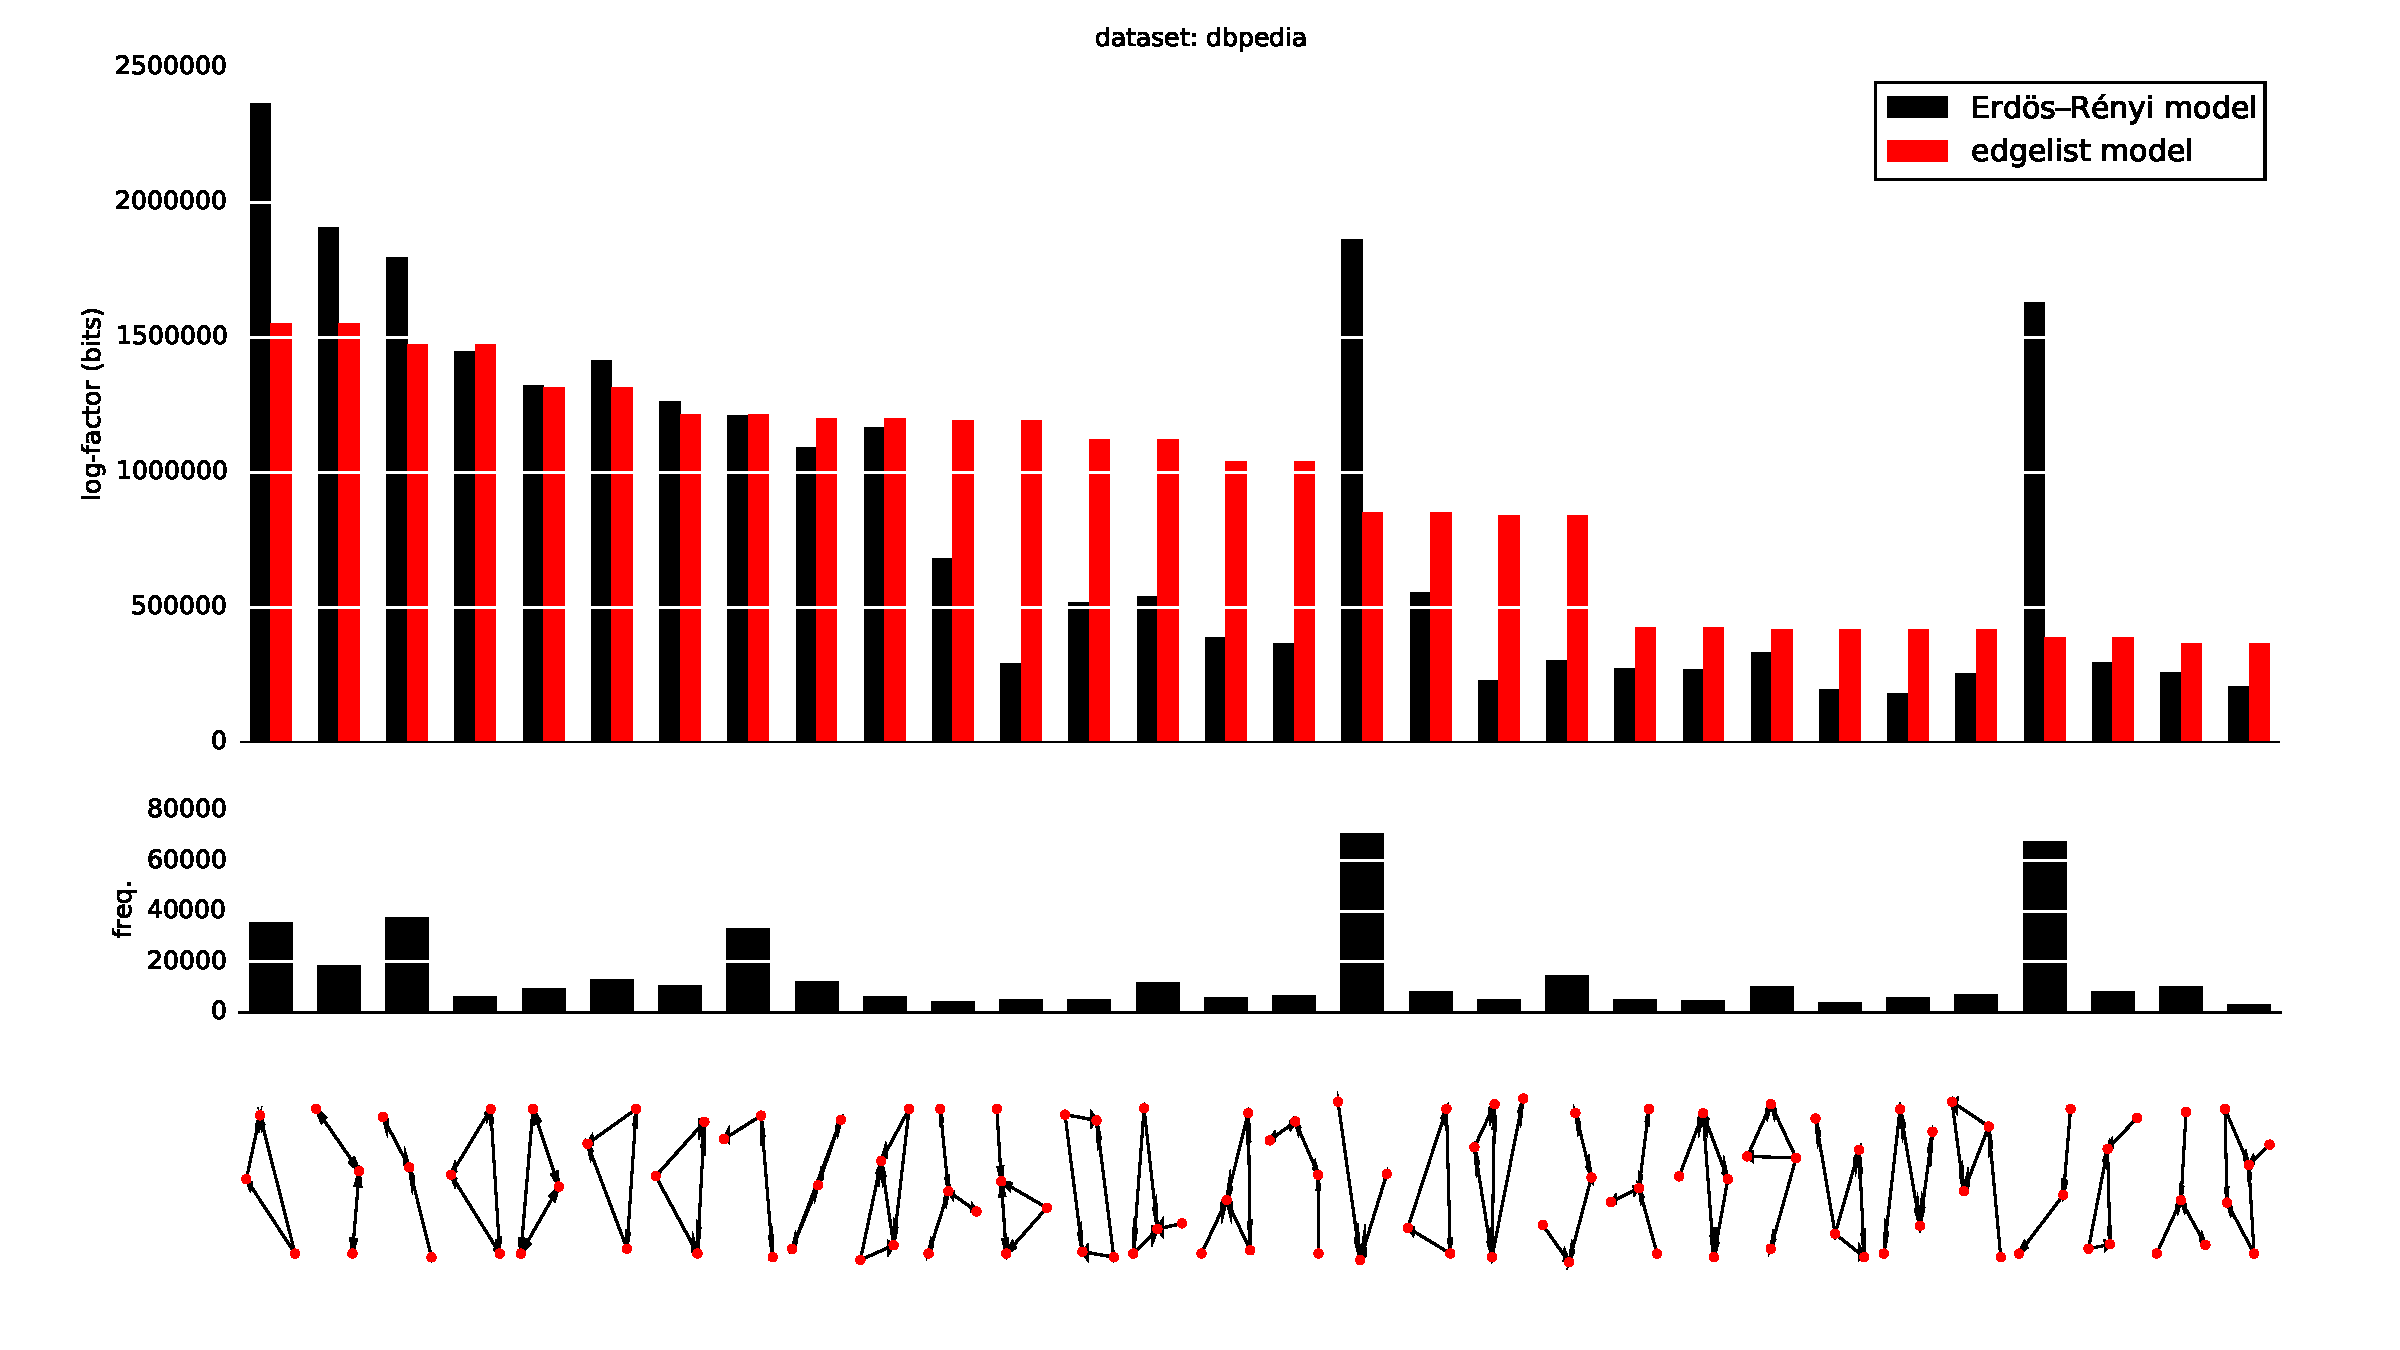
\includegraphics[width=\textwidth]{./images/large/compare-plot.pdf}
  \caption{The results of the motif extraction on a large-scale network. We show the thirty motifs with the highest log-factor under the EL model.}
  \label{figure:plot-large}
\end{figure*}

\section*{Conclusion} 

We have introduced a new method of testing motif relevance, which allows motif analysis to be scaled up to graphs with millions of nodes, even on commodity hardware. 

One observation from our experiments deserves further mention: in the first experiment, we saw that injection of one subgraph into a network caused other subgraphs to become motifs, ie. their frequencies became statistically significant. This tells us that even \emph{if} some motifs represent functional units of a network, as is often claimed (and contested) \cite{milo2002network,konagurthu2008origin}, the fact that a subgraph occurs with statistically significant regularity cannot be taken as proof that it is a functional unit. Hypothesis testing allows one to make a binary decision, but that decision is always \emph{about the null-model}. A low $p$-value should not be interpreted as evidence for the meaning of the subgraph. In fact, at this level of abstraction, the best any method can do is to offer sound \emph{candidates} for functional units. 

The proof that a particular motif actually corresponds to a meaningful unit can only be achieved in context: that is, a domain expert should evaluate the list of instances found for a particular motif, to see whether a large subset of them perform the same role in the network, or if not, what other reason can be found for the prevalence of the motif. In other words, motif analysis is necessarily an \emph{exploratory} technique, and while a significance test provides a good heuristic to separate trivially frequent subgraphs from subgraphs which may represent important properties, it is ultimately just a heuristic. The only thing it \emph{proves} is the incorrectness of the null-model. 

The reader may note that while we have shown that our method is fast in principle, if we wish to use the degree-sequence model, we are still limited to medium-scale graphs, and long processing times. There are several potential ways around this problem. First, the codelength for the whole graph is not specific to motif analysis. It only needs to be computed once for each $G$, after which it can be re-used in any MDL or Bayesian analysis (for motifs, cliques, clustering, etc.). Second, while we have chosen to use the null model also inside the motif model, this is not the only approach. We could also use the edgelist model in the motif code: since the edgelist code upperbounds the degree-sequence code, any positive log-factor in this setting means we would also get a positive log-factor if we used the degree-sequence model to store the motif and the template graph. There may also be efficient lowerbounds for the degree-sequence model, which we can use in its place for the null model. \footnotemark

\footnotetext{\cite{barvinok2010number} provides a lowerbound, but it cannot be computed much faster than the estimators used in our experiments. It may, however, be easier to parallelize.}

Our current model does not allow the detection of anti-motifs. For that purpose, another model would be required; one which exploits the property that a subgraph has a \emph{lower} frequency than expected to compress the data. In theory, this is certainly possible: any such non-randomness can be exploited for the purposes of compression. We leave this as a matter for future research.

Finally, we hope that our approach is illustrative of the general benefit of MDL techniques in the analysis of complex graphs. In conventional graph analysis a researcher often starts with a structural property that is observed in a graph, and then attempts to construct a process which generates graphs with that structural property. A case in point is the property of scale-freeness and the preferential attachment algorithm that was introduced to explain it \cite{albert2002statistical}. The Kraft inequality allows us instead to build models based on a description method for graphs. The trick then becomes to find a code that describes such graphs  with the desired property efficiently, instead of finding a process that is likely to generate such graphs. For many properties, such as cliques, motifs or specific degree sequences, such a code readily suggests itself. 


\label{chapter:motifs}
\chapter{An Expectation-Maximization algorithm for the fractal inverse problem}
\chaptermark{An EM algorithm for the inverse problem}


\begin{summary}
We present an expectation-maximization algorithm to solve the \emph{inverse problem} for iterated function systems (IFS): the task of fitting a fractal model to a given dataset. An IFS is defined by a small number of maps on $\mathbb{R}^H$, the IFS's \emph{components}. A point is sampled from the IFS by starting with some initial point and applying a sequence of randomly chosen components. The central idea of our algorithm is to treat this sequence as a latent variable. If we are given such a \emph{code} for each point in the data, we know which points should map to one another under each transformation of the IFS, allowing us to reconstruct the components. Given the components, we can easily assign codes each point. Iterating these two steps provides us with a basic algorithm to fit an IFS model to data.
\end{summary}

In the previous section, we met statisticians faced with graph data, and saw the envy they feel for their colleagues with tabular data who know exactly how to slice and dice their bitstrings. Their data is \emph{symmetrical under translation}: slide the bitstring a fixed number of bits to the left or right, and the data looks the same. Not exactly the same, of course, but the probability distribution over the instance we are looking at remains fixed.

As we saw, in analysing graphs we have very little idea of how to move our data so that the part we're looking at stays the same. Motifs provide one solution: if we look at one motif instance, and move the graph around so that we are facing another instance of the same motif, we have achieved a kind of symmetry. Not as clean as our smug colleagues with their tabular data, but it's a start at least.

There is, however, another kind of symmetry in graph data that is rarely used in tabular data: \emph{symmetry under re-scaling}. This principle is commonly used implicitly: no researcher actually has access to the entire web-graph. What is commonly used is a subgraph of the whole, extracted by crawling links on the web. All research using such datasets makes the implicit assumption that conclusions drawn on the basis of this subgraph also hold for the whole. A subgraph, some times much smaller than the full object under study, is assumed to be similar to the whole set.

This assumption may seem reasonable, but it can have some far reaching consequences. For instance, if the subgraph is like the whole in every respect, is a subgraph of the subgraph also like the subgraph, and thereby like the whole? Can the whole dataset be split in increasingly smaller sections that are all scaled down copies of the whole? The result is a fractal: a shape determined entirely by its self-similarity.

Fractals models have been popular since the seventies, when mathematicians and physicists began to realize that they could explain jagged, irregular features like coastlines, clouds and trees. Object that had been proving increasingly difficult to analyze with  classical Euclidean geometry. One problem that has always held back fractal analysis, however, is the inverse problem: we know how to draw pictures of a fractal model, but how to reconstruct the model given the picture?

To simplify the task, we investigate the problem in the domain of tabular data: we consider fractal datasets as points drawn independently from some self-similar distribution on a $d$-dimensional Euclidean space. We show that the inverse problem can be efficiently solved with Expectation-Maximization methods.

\section{Introduction}
What constitutes a fractal is not precisely defined. \footnotemark There are, however, three properties that are common to most objects that are described as fractals. First, there is \textbf{self similarity}: a part is a scaled down copy of the whole. See for instance the Sierpinski triangle (fig. \ref{figure:codes}). It consists of three triangular shapes which are scaled down copies of itself. Second, fractals tend to posess \textbf{infinitely fine structure}. 'Zooming in' reveals ever finer detail. In the case of the Sierpinski triangle, we will see the same shape recurring again and again, but other fractals like the Mandelbrot set reveal a great variety of shapes.
Finally, fractals tend to have \textbf{non-integer dimension}. The Sierpinski triangle, for example, has a Hausdorff dimension of $1.58$. 
 
\begin{figure}[b!]
  \centering
  \begin{subfigure}[b]{0.48\textwidth}
    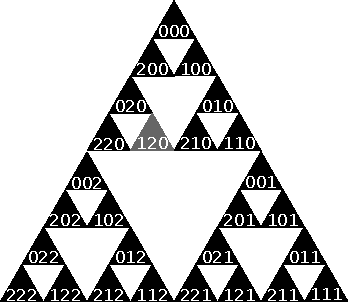
\includegraphics[width=\textwidth]{./images/sierpinski-codes.pdf}
    \caption{}
    \label{fig:sierpinski-codes}
  \end{subfigure}  
  \hspace{0.015\textwidth}
  \begin{subfigure}[b]{0.48\textwidth}
    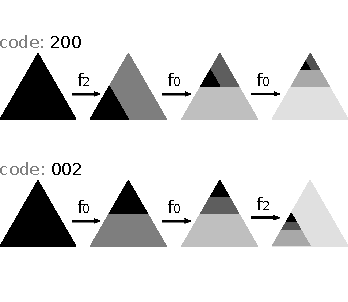
\includegraphics[width=\textwidth]{./images/code-construction.pdf}
    \caption{}
    \label{fig:code-construction}
  \end{subfigure}

  \caption{\small (a) Codes of length three on the Sierpinski triangle and the subsets they code for. (b) The construction of a subset from its code.}
  \label{figure:codes}
\end{figure}

Since the name fractal was coined in the 1970s, fractals have been seen as a potential model for many natural phenomena. Mandelbrot put it as follows in the \emph{The Fractal Geometry of Nature} \cite{mandelbrot1982fractal}:

\begin{quotation}
\small
\noindent Clouds are not spheres, mountains are not cones, coastlines are not circles, and bark is not smooth, nor does lightning travel in a straight line.
\end{quotation}

Fractal geometry has been used in many fields, including physics \cite{mandelbrot1984fractals}, geology \cite{cheng1997multifractal}, biology \cite{goldberger1992fractal} and economics \cite{turiel2003multifractal}.

One of the greatest problem with fractal analysis has always been the difficulty of finding a fractal model for a given set of data. It may be visually clear that a cloud or a coastline `looks' fractal, and we may be able to determine that it has a non-integer dimension, but how do we get from a dataset to a model? How do we determine the parameters of a fractal-generating model that lead to this particular dataset? Current approaches tend to rely on evolutionary algorithms \cite{deliu1991genetic}. Such algorithms take a long time, and it can be difficult to get them to converge to precise parameter values, even if the dataset itself is sampled from a fractal model.
Other approaches are highly domain-specific, such as fractal image compression \cite{hart1996fractal}. Some interesting results have been also been derived from the method of moments \cite{rinaldo1994inverse} and sampling random transformations from the data \cite{hart1997similarity}, but so far these have not led to a practical algorithm. 

\footnotetext{Mandelbrot originally defined it as a set whose topological dimension differs from its Hausdorff dimension, but retracted this definition, stating that he preferred the word to be not precisely defined.}

A very popular fractal model is the iterated function system (IFS). Many fractals, like the Sierpinski gasket, the Koch curve and the Menger sponge can be seen as IFSs. We will use the following definition:
\begin{definition}
An \emph{Iterated Function System} of order $K$ and dimension $H$ is a pair $(\{f_k\}, \{w_k\})$ of $K$ \emph{components} $f_k$ with $K$ associated \emph{weights} $w_k$. Each component is is a function $f_k: \R^H \to \R^H$, and each weight is a nonnegative scalar, with $\sum_i w_i = 1$. 
\end{definition}
In this paper, all components are similitudes: ie. $f_k$ is defined by a scalar $s_k$, a rotation matrix $R_k$ and a translation vector $t_k$:
\[
f_k(x) = s_kR_k x + t_k \p
\]
The definition can be extended to functions of any kind on metric spaces \cite{hutchinson2000deterministic}, but this formulation is sufficient for our purposes. 

The IFS determines a probability distribution on $\R_H$ in the following way. Let $p_0$ be some initial distribution on $\R^H$, whose support is a compact set, and let $D$ be some nonnegative integer. Let  $x_0 \sim p_0$. Let $x_1 \sim \sum_k  w_k f_k(x_0)$, that is, the distribution on $x_1$ is a mixture of the distribution on $x_0$ as transformed by the components. Let  $x_2 = \sum_k w_k f_k(x_1)$, and so on until $x_D$.

There are two basic properties to of IFSs. First, the distribution on $x_D$ converges with increasing $D$. We call the distribution it converges to the \emph{limit distribution}. Second, the limit distribution is independent of the choice of $p_0$. Thus, we can take the weights and components as \emph{parameters} that determine a distribution, and we can evaluate the IFS to high $D$ to approximate this ditribution. For formal statements of these properties and their proofs we refer the reader to \cite{hutchinson2000deterministic}. 

We can now frame the fractal inverse problem as a problem of statistical parameter estimation: we would like to find the IFS for which the probability of of the data under its limit distribution is maximal. The algorithm we describe is based on the following ideas:
\begin{itemize}
  \item Since the initial distribution doesn't matter, we can choose what we like. We choose the standard multivariate Normal (MVN) distribution $\cN_0$. The benefit of this choice is that every affine transformation of an MVN is itself an MVN. Thus, no matter how high we set $D$, the resulting distribution will always be a mixture of MVNs. 
  \item We assume that each point in the dataset was the result of a sequence of applications of the components of the model. We cast this sequence---called a \emph{code} hereafter---as a latent variable in our model. Each code $c$ determines an \emph{endpoint distribution}, and each endpoint distribution is an MVN $\cN_c$.
  \item  Given the IFS that generated our data, it is a simple matter to find the most likely code for each point $x$. Conversely, if we know the most likely code for each datapoint, we can determine which points in the dataset should map to one another, under a particular component $f_k$. This correspondence allows us to reconstruct $f_k$.    
\end{itemize}

We make the correspondences in the last point probabilistic: instead of assigning each point its most likely code, we compute a \emph{responsibility} that each possible component takes for the point. This is the posterior probability of the component given the point: $p(c \mid x) \propto p(x \mid c) p(c)$, where $p(x\mid c) = N_c(x)$ and $p(x) = \prod_{s \in c} w_s$. This is the \emph{expectation} step of the algorithm. The \emph{maximization} step, optimizing the IFS model given these probabilities is detailed in the body of the paper. 

Note that finding a code corresponding to a particular endpoint can be counter-intuitive, as the first component applied determines the location at the smallest scale, and the last component applied determines the location at the largest scale. Figure~\ref{figure:codes} provides an illustration.

We show in Section~\ref{section:experiments} that our algorithm quickly reconstructs known fractals, such as the Sierpinski gasket and the Koch curve. We also apply the algorithm to some datasets sampled from images, and some natural data of higher dimension, showing that, while there are no IFSs to perfectly capture these images, the self similarity in the model does often allow a better fit than a simple mixture of MVNs.

\subsection{Preliminaries}
\paragraph{Measures and transformations} Let $\{x_i\}_{i\in[1,N]}$, $x_i\in\R^H$ be our dataset. Let $X$ be the $N\times H$ matrix with $x_i$ as its columns. All vectors are column vectors.  

Let $1_L$ be the length-$L$ vector with $1$ at all indices. Such vectors are useful tools in matrix notation: for instance, the sum of the elements of the $K \times L$ matrix $M$ can be expressed as ${1_K}^T M 1_L$, while its marginal vectors are $({1_K}^T M)^T$ and $M 1_L$. Let $0_L^j$ be the length-$M$ vector with element $j$ $1$ and all others $1$. This vector functions as a row- or column-selector, eg. $X 0^j_N = x_i$.

Let $v(X)$ be a probability distribution with $X \subseteq \R^H$. Let $f_{t, A}(x) = Ax + t$ be an invertible affine transformation represented by a vector $t$ and a matrix $A$. Then the transformation of $v$ by $f_{t, A}$ is defined by the relation $f_{t, A}(v)(X) = v({f_{t, A}}^{-1}(X))$. Let $v(x)$ be the density function of  the measure $v$ (with respect to the Lebesgue measure). Then the density function of the measure $f_{t, A}(v)$ is $f_{t, A}(v)(x) = |A^{-1}| v({f_{t, A}}^{-1}(x))$.

A multivariate normal distribution (MVN) on $\R^H$ is determined by a mean $\mu \in \R_H$ and a covariance matrix $\Sigma \in \R^{H\times H}$. Its probability density function is:
\[
\cN(x \mid \mu, \Sigma) = (2\pi)^{-\frac{H}{2}}|\Sigma|^{-\frac{1}{2}} \exp \left [-\frac{1}{2} \left \| (x-\mu)^T\Sigma^{-1}(x-\mu) \right\|^2\right] 
\]
We will call the MVN with $\mu = 0$, $\Sigma = I_H$ the standard multivariate normal distribution, or $\cN_0$. A \emph{spherical MVN} has $\Sigma = sI$ for some scalar $s$. Let $x$ be random variable with $x \sim \cN(\mu, \Sigma)$, then $f_{t, A}(x) \sim \cN(t + A\mu, A\Sigma A^T)$. 

A \emph{rotation matrix} $R$ is a matrix with $R_R = I$ and $|R| = 1$. A \emph{similitude} (or rigid transformation) on $\R^H$ is a transformation defined by a rotation matrix $R \in \R^{H\times H}$, a translation vector $t \in \R^H$ and uniform scaling $s \in R$: $f_{t, R, s}(x) = sRx + t$. 
The inverse of a similitude is also a similitude: ${f_{s, R, t}}^{-1}(x) = f_{\frac{1}{s}, R^T, -\frac{1}{s}R^Tt}(x)$.

$f_{s, R, t}(\cN_0)$ is a spherical MVN with mean $t$ and covariance $s^2I$. Transforming a generic spherical MVN by a similitude can be cast as the transformation of $\cN_0$ by two similitudes:
\begin{align}
f_{t, R, s}(\cN_{t_0, {s_0}^2 I})(x) &= f_{t, R, s}(f_{t_0, R_0, s_0}(\cN_0))(x) \notag \\
&=  (2\pi)^{-\frac{H}{2}} ({ss_0})^{-H} \exp \left[- \frac{1}{2{s_0}^2s^2}\left\| x - (s R t_0 + t)\right \|^2\right] \label{line:inverse}
\end{align}
\paragraph{The EM Algorithm} \cite{dempster1977maximum}
Let $p(X\mid Z, \theta)$ be probability distribution with parameters $\theta$ and latent variables $z$. In the most common oexample of the EM algorithm, $p$ is a mixture of MVNs: $\theta$ contains the parameters of $K$ MVNs together with a weight $w_k$ for each. $Z$ is a matrix whose rows $z_i$ determine which component is responsible for $x_i$: ie. if component $k$ is responsible, then $Z_{ik}$ is 1 and all other elements of row $i$ are 0.

The maximum likelihood parameters for a dataset $X$ are determined by 
\[
\argmax_{\theta} \ln p(X|\theta) = \argmax_{\theta} \ln \sum_Z p(X|Z, \theta)p(Z) 
\]
where the sum is over all possible values of $Z$. The value inside the sum is the \emph{complete-data likelihood} $p(X, Z\mid \theta)$. In the mixture-of-MVNs example, there are $K^N$ possibilities for $Z$, making this sum intractable for practical data. 
 
The intuition behind EM is to optimize $\theta$ with respect to our best guess for $Z$ and vice versa. Let $\theta^\text{old}$ be our current best guess for the parameters. We first optimize $p(Z\mid X, \theta^\text{old})$, the posterior on the latent variables. Note that, in the MVN example, we can represent this as an $N\times K$ matrix $Z$ with $Z_{ij} = p(j\mid x,\theta) = N^\text{old}_j(x) w_j$. These are known as the \emph{responsibilities}.

We then determine the expectation of the logarithmic complete-data likelihood under  our posterior $p(Z|X, \theta^\text{old})$ as a function of $\theta$.
\[
Q(\theta) = \sum_Z p(X|Z, \theta^\text{old})p(Z) \ln p(X, Z \mid \theta)
\]  
Note that the complete-data likelihood is now inside the logarithm. We optimize this \emph{$Q$-function}, with respect to $\theta$:
\[
\theta^\text{new} = \argmax_\theta Q(\theta)\p
\]
 The computation of the matrix $Z$ is know as the \emph{expectation} step and the computation of $\theta^\text{new}$ is known as the \emph{maximization} step. The EM algorithm iterates the two steps until the parameters converge.

\section{The IFS model}

\begin{figure*}[t]
  \center
  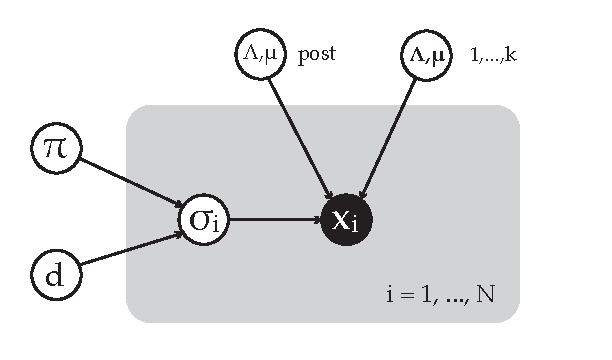
\includegraphics[width=0.7\textwidth]{./images/factor-graph.pdf}
  \caption{A graphical model, illustrating the components of the IFS model. The gray box is a plate, representing a repetition of the nodes inside the box for each datapoint. The black node represents the observed data.}
  \label{figure:ifs-diagram}
\end{figure*}

The complete IFS model is illustrated in Figure~\ref{figure:ifs-diagram}. It consists of:
\begin{description}
\item[the depth  priors $v$] The number of times the IFS is iterated for each point. $v$ is a vector representing a categorical distribution on $[0,D]$, from which the length of the code $c$ is sampled.
\item[the component weights $w$] This is a vector of $K$ non-negative real values, with $\sum_k w_k = 1$. Each weight determines the probability of its associated component being chosen at each iteration of the IFS.
\item[the components $f_k = \{s_k, R_k, t_k\}$] $K$ similitudes. 
\item[The post-transformation $s_p, R_p, t_p$] The parameters a single \emph{post-transformation}. This transformation is applied once to all sampled points.
\item[The code $c_i$] An ordered sequence $c_i = \langle c_{i1}, \ldots, c_{id} \rangle$. Each element of the code is an integer in $[1,K]$ representing a component. 
\item[The data $x_i$] This is the point after the post-transformation is applied: ie. the observed data.
\end{description}

To sample a point $x_i$ from this model we first sample a depth $d$ with $p(d=a) = v_a$. We then sample a sequence $c_j$ of $d$ components $c_{i1}, \ldots, c_{id}$ with each $c_ji \in [1,K]$ chosen independently with $p(c_{ji} = a) = w_a$. We then create the composite function $f = f_p \circ f_{c_{j1}} \circ \ldots \circ f_{c_{jd}}$ and sample $x$ from $f(\cN_0)$. Equivalently, we can sample $x_0$ from $\cN_0$ and apply the components prescribed by $c_i$ in series, and then apply $f_p$.

Giving the model a variable depth has several advantages. First, it makes the model a generalization of good fall-back models. With $v_0 = 1$, the model becomes a spherical multivariate Gaussian. With $v_1 = 1$, the model becomes a mixture of spherical Gaussians.\footnotemark Since each point has its own depth, the full model is a mixture over all these models, and the deeper IFS models. If the data is not self similar, or only partially self similar (like an IFS model with outliers), the lower depth parts of the mixture can account for this.

The variable depth also allows the EM search a `gentle start'. In the limit, most IFSs have a support with lower dimension than the embedding dimension of the data: ie. almost all of $\R^H$ has probability zero. This means that even if the model fits the source of the data perfectly, the slightest addition of noise will make the entire likelihood zero. It also means that a minute change in parameters can mean the difference between the maximum likelihood, and likelihood zero. In effect, for high values of $d$, the fitness landscape becomes very jagged. 

The depth parameters provide an automatic defense: if such a drop occurs, the lower models, whose fitness landscape is smoother, automatically get a higher posterior, smoothing out the fitness landscape for the complete mixture. As the search converges to the correct model, the depth prior becomes more weighted towards the higher depths.

However, the variable depth also creates a problem when our data is not perfectly centered. If we transform an IFS, evaluated to depth $d$, by an affine transformation, the result is also an IFS. However, the resulting components depend on $d$. Imagine a dataset sampled from a Sierpinski gasket translated away form the origin. We have good models at every depth for this data, but their components are different. Only if the data is centered do the components coincide for all depths. This is desirable, because once the solution has converged to these components, we will see the higher depths gaining more weight. But how the data should be centered for the components to coincide differs from one IFS to another. This is the reason for the \emph{post-transform}: we learn a centered IFS, and transform it to the data.   

\footnotetext{To generalize to non-spherical MVNs and mixtures over non-spherical MVNs, the component family should be extended to positive definite affine functions. This extension is discussed in the conclusion.}

\section{The EM algorithm for IFS models}

We will use the notation $[1,K]^d$ to refer to the set of all length-$d$ codes. Let $[1,K]^{[a,b]} = \bigcup_{d \in [a,b]} [1,K]^d$. Thus, the set of all codes, including the empty code, is $[1, K]^{[0, D]}$. For every code $c_j$ in this set, we have 
\begin{align*} 
p(x \mid c_j) &= \cN(x \mid \mu_j, \Sigma_j) \\
p(c_j) &= p(d) \prod_i p(c_j) = v_{|c_j|}\prod_{i \in c_j} w_{i}
\end{align*}

Where $\mu_j$ is the mean corresponding to $f_j(\cN_0)$ with $f_j = f_p \circ f_{c_{j1}} \circ f_{c_{j2}} \circ \ldots \circ f_{c_{jd}}$, and $\Sigma_j$ is the covariance matrix $f_j(\cN_0)$.

\subsection{Expectation: the latent variables}

The responsibilities for an MVN mixture model are well-known. Let $M = |[1, K]^{[0, D]}|$ and let $P$ be an $N\times M$ matrix with: 
\[
P_{ij} = p(c_j \mid x_i) = \frac{p(x_i\mid c_j) p(c_j) }{\sum_{a \in [1,K]^{[0, D]}} p(x_i\mid c_a) p(c_a)} \p 
\]
We also define a specific matrix for each $f_k$ for purposes that will become clear in the next section. Let $M = |[1, K]^{[0, D-1}]|$, and let $P^k$ be an $N \times M$ matrix with: 
\[
P_{ij}^k = p(k.c_j \mid x_i) = \frac{p(x_i\mid k.c_j) p(k.c_j) }{\sum_{a \in [1,K]^{[0, D]}} p(x_i\mid c_a) p(c_a)} 
\]
where $k.c_j$ is the code $\langle k, c_{j1}, \ldots\rangle$. Note that this is a sub-matrix of $P$.

The size of these matrices will grow very fast with $D$, and most of its values will be practically indistinguishable from $0$ when normalized. For this reason, it may be advisable to set all but the largest values to $0$, and store the matrix in a sparse datastructure. For our experiments, such optimizations were not necessary.

\subsection{Maximization: the parameters}

Let $\theta^\text{old}$ be the model we used to compute the responsibilities. Our $Q$-function is:
\begin{align*}
Q(\theta) &= \sum_{i} p(z_i \mid x_i, \theta^\text{old}) \ln p(x_i \mid z_i, \theta) p (z_i \mid \theta) \\
     &= \sum_{i=1,j=1}^{N, M} P_{ij} \ln \cN_j(x) \;v_{|c_j|}\; \prod_{a\in c_j}w_a \,\,\, \text{with } M = |[1,K]^{[0,D]}|
\end{align*}

For clarity of notation, when optimizing for a certain subset of the parameters $q$ (such as the depths, weights or parts of the components) we will write $Q(q)$, and omit any terms that are constant with respect to $q$. We may also omit any constant multiplier of the whole function.

To find the optimal depth we solve $\partial Q(v)/\partial v$, using a Lagrange multiplier to enforce that $v$ sums to one, which gives us:
\[
\hat v_d = \frac{p_d}{\sum_i p_i} \,\,\text{with } p_d = \sum_{j: |c_j| = d} P_{ij}
\]

\paragraph{The components $f_k$ and weights $w_k$}

Even with the simplifications of the EM algorithm $Q$ is very difficult to optimize for $f_k$ and $f_p$. We must find $K$ maps and weights, and a post-transformation $f_p$, such that all the $M$ endpoint distributions, provide maximal likelihood to their assigned points. The problem is that each term in $Q$ is a complicated mix of multiple components.

To make the optimization of $Q$ practical, we simplify the task in two ways. First, we optimize $f_p$ and $(\{f_k\}, \{w_k\})$ separately, taking the parameters not being optimized from $F^\text{old}$. Let $Y = {f_p^\text{old}}^{-1}(X)$. Second, we simplify the $Q$ function as follows: 

\begin{align*}
Q(\{f_k\}, \{w_k\}) = \sum_k \sum_{i=1,j=1}^{N, M} & p(k.c_j \mid x, F^\text{old}) \ln f_p f_k(\cN_{j})(x_i) p^{\text{old}}(c_j) p(k)\\ & \hfill \text{with } M = |[1,K]^{[0, D-1]}|  \\
= \frac{1}{s^\text{old}_p}\sum_k \sum_{i, j} &P^k_{ij} \ln \left[ f_k(\cN_{j})(y_i) \; v_{|c_j|+1} p(c_j) \; w_k \right]\p
\end{align*}
We then \emph{approximate} all elements indexed by $j$, so that of all the transformations in each code, only the last one functions as an argument of $Q$. We approxiamte $\cN_j$ by computing it from the model $\theta^\text{old}$.

This gives us:
\begin{align*}
Q(f_k, w_k) &= \sum_{i, j} P^k_{ij} \ln f_k(\cN_j)(y_i) + \sum_{i, j} P^k_{ij} \ln w_k  
\end{align*}
Finding $w_k$ follows the same principle as the depths. We find:
\[
\hat w_k = p^k / \sum_{i} p^i \p
\]
with $p^k = {1_N}^TP^k1_M$, the sum of the elements of $P^k$.

If we isolate $f_k$, the problem is very similar to the one solved to construct the Coherent Point Drift (CPD) algorithm \cite{myronenko2010point}: transform a set of MVNs to maximize the likelihood of a dataset, with respect to responsibilities $P$. The main difference is that in our situation each component $N_j$ has its own variance. We follow the same approach, and as we shall see, the solutions for our problem are very similar to those of the CPD algorithm.

Using Equation~\ref{line:inverse} from the preliminaries, we can rewrite $Q(f_k)$ as a mixture of transformations of $\cN_0$:
\begin{align*} 
Q(s_k, R_k, t_k) &= - p^k H \ln s_k - \sum_{i, j} P^k_{ij} \frac{1}{2{s_j}^2{s_k}^2} \left\|y_i-t_k - s_k R_k t_j \right\|^2 
\end{align*}
where $s_j$, $R_j$ and $t_j$ are the parameters of the similitude $f_p \circ c_{j1} \circ \ldots \circ c_{jd}$. 

To find the optimal translation $t_k$, we solve $\partial Q(t_k)/\partial t_k = 0$, which yields, in matrix notation:
\begin{align*}
\hat t_k &= \frac{1}{p^k_z}YP^kZ1_M - \frac{1}{p^k_z}s_kR_kTZ{P^k}^T1_N = y^k - s_kR_k t^k
\end{align*} 
where $T$ is the matrix with $t_j$ as its columns, $Z = \text{diag}({s_1}^{-2}, \ldots, {s_M}^{-2})$ and ${p^k_z} = {1_N}^TP^kZ1_M$, the sum of the elements of the matrix $P^kZ$. Thus $\hat t_k$ is the difference between a weighted mean of the data $y^k$ and a weighted mean of the endpoint means $t_j$, scaled and rotated, where in both cases, the matrix  $P^kZ$, normalized to sum to one, determines the weights. Note that this is not a complete solution, since it still depends on $s_k$ and $R_k$. We can, however, plug $\hat t_k$ back into the $Q$-function to optimize for $R_k$.

Finding the optimal rotation matrix $R_k$ is more complex than simply finding the derivative and setting it equal to zero, since we have the constraint that $R_k$ is orthogonal and has determinant $1$. We use the technique described in \ref{myronenko2009closed} and \cite[Lemma~1]{myronenko2010point}. We first rewrite the objective function to the form $\text{tr}(A^TR_k)$, for some $A$. We fill in $\hat t_k$, and reduce to
\[ 
Q(R_k) = \text{tr}\left(\left[\ol{Y}^kP^kZ{\ol{T}^k}^T\right]^TR_k\right) 
\]
with 
\begin{align*}
\ol{Y}^k &= Y - y^k {1_N}^T\\
\ol{T}^k &= T^k - t^k {1_M}^T\\
\end{align*}
The optimal $R_k$ can be derived from the singular value decomposition (SVD) of $A=\ol{Y}^kP^kZ{\ol{T}^k}^T$: if $A = USV^T$, with $U$, $S$ and $V$ defined as normal for the SVD then we have $\hat R_k = U \;\text{diag} (1, \ldots, 1, |UV^T|)\; V^T$.

Finally, we derive the scaling parameter $s_k$ by filling in $\hat t_k$ and solving $\partial Q(S_k)/\partial s_k$. We get:

\begin{align*}
0 &= {s_k}^{-2}\;\text{tr}({\ol{Y}^k}^T\text{diag}(P^kZ1_M)\ol{Y}^k) + {s_k}^{-1}\;\text{tr}(\ol{T}^kZ{P^k}^T{\ol{Y}^k}^TR_k) -H p^k \p
\end{align*}
This is a quadratic polynomial in ${s_k}^{-1}$, which we can solve and invert to find $\hat s_k$.

\subsection{The post transform: $s_p$, $R_p$, $t_p$} Let $M = \left |[1,K]^{[0,D]}\right|$ The $Q$-function becomes:
\begin{align*}
Q(s_p, R_p, t_p) &= \sum_{i=1,j=1}^{N,M} p(c_j\mid x_i) \ln f_p(N_j)(x_i) p(c_j) \\
&= - p\ln s_p  - \frac{1}{2 {s_p}^2} \sum_{i, j} {s_j}^{-2} P_{ij} \| x - t_p -s_pR_pt_j \|^2 \\
\end{align*}
where $p = {1_N}^T P 1^M$ and $s_j$ and $t_j$ can be derived from the optimal components, as determined above. Note that $j$ now iterates over a larger set of codes.

The form of the $Q$ function is the same as the ones we used to derive the optimal components $s_k, R_k, t_k$. We follow the same derivations and get: 

\begin{align*}
\hat t_p &= \overline{x} - s_pR_p\overline{t}\\
\hat R_p &= U\;\text{diag}(1, \ldots, 1, |UV^T|)\;V^T & \text{with } USV = \text{svd}(A), A = \ol{X} P Z {\ol{T}}^T \\
\end{align*}
with 
\begin{align*}
\ol{x} &= ({1_N}^TPZ1_M)^{-1} XPZ1_M & & \ol{t} = ({1_N}^TPZ1_M)^{-1}TZP^T1_M\\
\ol{X} &= X - \overline{x}{1_N}^T & &\ol{T} = T - \overline{t} {1_M}^T\\
Z &= \text{diag}({s_1}^{-2}, \ldots, {s_M}^{-2})\\
\end{align*}

Finally, for $s_p$, we solve
\[
0 = {s_p}^{-2}\text{tr}(\ol{X}^T\text{d}(PZ1_M)\ol{X}) + {s_p}^{-1} \text{tr}(\ol{T}ZP^T\ol{X}^TR_p) - H p
\]

\begin{pseudo}[th]
\caption{One iteration of the EM algorithm for fitting a fractal model.}
{
Given: a dataset $X$, a number of components $K$, a maximum depth $D$. \\

$C \leftarrow [0,K]^{[0, D-1]}$, $M \leftarrow |C|$ \emph{\# the set of all codes of length up to $D$} \\
\emph{\# Expectation step}\\
$P_{ij} \leftarrow N_j(x_i) p(d) \prod_{c \in [1,K]^d} w_c$  \\ 
Normalize $P$ so that $P1_M = 1_N$ \\
\textbf{for each} $k \in [1,K]$: \\
\tab Let $P^k$ be the submatrix of $P$'s columns $j$ such that $c_{j1} = k$\\
\\
\emph{\# Maximization step} \\
$Y \leftarrow {f^\text{old}_p}^{-1}(X)$\\
for all $d$, $v_d \propto \sum_{j : |c_j| = d} P_{ij} $\\
\textbf{for each} $k \in [1,K]$: \\
\tab $w_k \leftarrow {1_N}^T P^k 1_M / \sum_i {{1_N}^T P^i 1_M}$\\
\tab $y^k \leftarrow {p^k}^{-1}YP^kZ1_M, \,\,\, t^k \leftarrow {p^k}^{-1} T^kZ{P^k}^T 1_N$\\
\tab $\ol{Y}^k \leftarrow Y + y^k{1_N}^T$, \,\,\, $\ol{T}^k \leftarrow T^k + t^k{1_M}^T$\\
\tab $Z \leftarrow \text{diag}({s_1}^{-2}, \ldots, {s_M}^{-2})$\\
\tab $U,S,V^T \leftarrow \text{svd}(\ol{Y}^kP^kZ{\ol{T}^k}^T)$\\ 
\tab $R_k \leftarrow U\;\text{diag}(1,\ldots,1,|UV^T|) V^T$ \\
\tab $s_k$: solve ${s_k}^{-2}\; \text{tr}({\ol{Y}^k}^T\text{d}(P^kZ1_M)\ol{Y}^k) + {s_k}^{-1}\;\text{tr}(\ol{T}^kZ{P^k}^T{\ol{Y}^k}^TR_k) - Hp^k= 0$ \\
\tab $t_k \leftarrow y^k - s_k R_k t^k$ \\

$C \leftarrow [0,K]^{[0, D]}$, $M \leftarrow |C|$\\
$X' \leftarrow X - \overline{x}{1_N}^T$, $T' \leftarrow T + \overline{t}{1_M}^T$\\
\tab $Z \leftarrow \text{diag}({s_1}^{-2}, \ldots, {s_M}^{-2})$\\
$U,S,V^T \leftarrow \text{svd}(X'PZ{T'}^T)$\\ 
$R_p \leftarrow U\;\text{diag}(1,\ldots,1,|UV^T|) V^T$ \\
$s_p$: solve ${s_p}^{-2}\text{tr}(X'PZ1_NX'+ T'Z{P}^T1_MT') - s_p^{-1} \text{tr}(ZP^T{x'}^TT') -Hp = 0$ \\
$t_p \leftarrow \overline{x} - s_pR_p\overline{t}$ \\
}
\end{pseudo}

\subsection{Dealing with singularities}

In the EM algorithm for MVN mixtures, there is a danger that the algorithm becomes stuck in a situation where one or more of the components do not have responsibility for any part of the data, or for only a single point. In this case, the covariance matrix for such components cannot be computed, and the algorithm must be reset in some way.

In the IFS algorithm a similar thing can happen, causing one or more of the matrices $P^k$ to become low-rank. In this case, the SVD decomposition required to find $R_k$ cannot be computed. When this happens, we use the following strategy: we remove the undetermined component, and for each one we \emph{split} one of the well-determined components. Let $f_a = (s_a, R_a, t_a)$ with weight be the well-determined component and $f_b$ be the singleton component. We resolve the situation by setting:
\begin{align*}
f_a \leftarrow (s_a, R_a, t_a + \epsilon_a)\\
f_b \leftarrow (s_a, R_a, t_a + \epsilon_b) 
\end{align*}
where $\epsilon_a, \epsilon_b$ are vectors with elements randomly drawn from $\cN(0, \sigma)$, where we use $\sigma = 0.001$ in all experiments. The weight $w_a$ is distributed equally over the components $f_a$ and $f_b$ and the weight vector is re-normalized.
 
The rationale is easiest to understand if we take $v_1=1$ and view the model as a mixture of Guassians. In that case, the well-determined components cover all the data. By splitting $f_a$, and adding some small noise, the points formerly `claimed' by $f_a$ will now be distributed approximately evenly between $f_a$ and $f_b$. 

A second trap is that the variance of the endpoint distributions can become so small that, even using logarithmic representation, the matrices $P^k$ become low-rank (ie, all entries are $0$) for certain components. If this happens, we reset the algorithm by approximating $P$  and all $P^k$: we still use the endpoint means $t_j$ from the model, but we place an MVN with a fixed standard deviation on each (we use the standard deviation 0.01 in all experiments) and re-compute the responsibilities under that model.

\section{Results}
\label{section:experiments}

To speed up the algorithm, we us a subsample (with replacement) from the data in all experiments. After each iteration (one expectation and one maximization step), we draw another sample. The sample size is always 250. We run the algorithm for 300 iterations, with maximum depth 5. In practice, it may be advisable to increase the sample size and the depth as the algorithm begins to converge, but for the sake of simplicity, we have kept the parameters fixed.

\subsection{Synthetic distributions}
\begin{figure*}
\begin{tabular}{c c c c c}
\hline
data & it. 20 & it. 40 & it. 250 & full depth \\
\hline
    \includegraphics[width=0.2\textwidth]{{./images/fractals/sierpinski/workspace/fractal/0/data}.pdf} & 
    \includegraphics[width=0.2\textwidth]{{./images/fractals/sierpinski/workspace/fractal/0/best/iteration.000020}.pdf} & 
    \includegraphics[width=0.2\textwidth]{{./images/fractals/sierpinski/workspace/fractal/0/best/iteration.000040}.pdf} & 
    \includegraphics[width=0.2\textwidth]{{./images/fractals/sierpinski/workspace/fractal/0/best/iteration.000299}.pdf} &
    \includegraphics[width=0.2\textwidth]{{./images/fractals/sierpinski/workspace/fractal/0/best/iteration.000299.deep}.pdf} \\ 
    \includegraphics[width=0.2\textwidth]{{./images/fractals/sierpinski-off/workspace/fractal/0/data}.pdf} & 
    \includegraphics[width=0.2\textwidth]{{./images/fractals/sierpinski-off/workspace/fractal/0/best/iteration.000020}.pdf} & 
    \includegraphics[width=0.2\textwidth]{{./images/fractals/sierpinski-off/workspace/fractal/0/best/iteration.000040}.pdf} & 
    \includegraphics[width=0.2\textwidth]{{./images/fractals/sierpinski-off/workspace/fractal/0/best/iteration.000299}.pdf} & 
    \includegraphics[width=0.2\textwidth]{{./images/fractals/sierpinski-off/workspace/fractal/0/best/iteration.000299.deep}.pdf} \\ 
	\includegraphics[width=0.2\textwidth]{{./images/fractals/koch2/workspace/fractal/0/data}.pdf} & 
    \includegraphics[width=0.2\textwidth]{{./images/fractals/koch2/workspace/fractal/0/best/iteration.000020}.pdf} & 
    \includegraphics[width=0.2\textwidth]{{./images/fractals/koch2/workspace/fractal/0/best/iteration.000040}.pdf} & 
    \includegraphics[width=0.2\textwidth]{{./images/fractals/koch2/workspace/fractal/0/best/iteration.000299}.pdf} & 
    \includegraphics[width=0.2\textwidth]{{./images/fractals/koch2/workspace/fractal/0/best/iteration.000299.deep}.pdf} \\ 
	\includegraphics[width=0.2\textwidth]{{./images/fractals/koch4/workspace/fractal/0/data}.pdf} & 
    \includegraphics[width=0.2\textwidth]{{./images/fractals/koch4/workspace/fractal/0/best/iteration.000020}.pdf} & 
    \includegraphics[width=0.2\textwidth]{{./images/fractals/koch4/workspace/fractal/0/best/iteration.000040}.pdf} & 
    \includegraphics[width=0.2\textwidth]{{./images/fractals/koch4/workspace/fractal/0/best/iteration.000299}.pdf} & 
    \includegraphics[width=0.2\textwidth]{{./images/fractals/koch4/workspace/fractal/0/best/iteration.000299.deep}.pdf} \\ 
	\includegraphics[width=0.2\textwidth]{{./images/fractals/sierpinski2/workspace/fractal/0/data}.pdf} & 
    \includegraphics[width=0.2\textwidth]{{./images/fractals/sierpinski2/workspace/fractal/0/best/iteration.000020}.pdf} & 
    \includegraphics[width=0.2\textwidth]{{./images/fractals/sierpinski2/workspace/fractal/0/best/iteration.000040}.pdf} & 
    \includegraphics[width=0.2\textwidth]{{./images/fractals/sierpinski2/workspace/fractal/0/best/iteration.000299}.pdf} & 
    \includegraphics[width=0.2\textwidth]{{./images/fractals/sierpinski2/workspace/fractal/0/best/iteration.000299.deep}.pdf} \\
\hline 
\end{tabular}  
  \caption{Results of EM search for known models. The red and blue boxes show the model: the post-transform maps the image frame onto the red box, and each component maps the red box onto a blue box. The bars in the side of the blue boxes show the weight of each component. The learning tasks, from top to bottom are: the Sierpinski gasket, the Sierpinski gasket with unequel weights, the Koch curve with 4 components, the Koch curve with two components and the Sierpinski gasket with two components.}
  \label{figure:synthetic}
\end{figure*}

Figure~\ref{figure:synthetic} shows the performance of the algorithm on four well known fractals: the Sierpinski gasket, a Sierpinski gasket with unequal weights, and two- and four-component versions of the Koch curve.

For each dataset we repeated the experiment 100 times and both the model with its learned mixture over depths, and what the IFS looks like when evaluated to infinite depth. \footnotemark We show the run that ended with a model with the greatest likelihood (on the training data). the end results of all runs are shown in the appendix. 

\footnotetext{Such data can be sampled using an algorithm known as the \emph{chaos game} \cite{barnsley2014fractals}.}
 
It is difficult to objectively quantify the number of trials that successfully converged to the required IFS. One may suggest testing the likelihood of the data under the learned model, to see if it is close to that of the target model, but the likelihood grows exponentially as the higher depths get greater weight (if the model is correct). This means that unless the algorithm finds the absolute correct model, the likelihoods of any learned model, correct or otherwise, will be much closer to one another than to the likelihood of the target model.  

We inspected the resulting models for each of the 100 runs visually to determine whether they were good approximations, and report the proportions here, with the proviso that these necessarily include some level of subjective judgment. The complete set of results for each experiment is reproduced in the appendix. 

We observe that the most difficult of these models appears to be two-component Koch curve. This is most likely due to the fact that the components of this model require an exact rotation. Compare this to the Sierpinski triangle, where each component can have a rotation of 0, 120 or 240 degrees, without changing the model.

\subsection{Non IFS data}

\begin{figure*}
\begin{tabular}{c c c c c}
\hline
data & it. 20 & it. 40 & final model & full depth \\
\hline
    \includegraphics[width=0.2\textwidth]{{./images/fractals/cloud/workspace/fractal/0/data}.pdf} & 
    \includegraphics[width=0.2\textwidth]{{./images/fractals/cloud/workspace/fractal/0/best/iteration.000020}.pdf} & 
    \includegraphics[width=0.2\textwidth]{{./images/fractals/cloud/workspace/fractal/0/best/iteration.000040}.pdf} & 
    \includegraphics[width=0.2\textwidth]{{./images/fractals/cloud/workspace/fractal/0/best/iteration.000299}.pdf} &
    \includegraphics[width=0.2\textwidth]{{./images/fractals/cloud/workspace/fractal/0/best/iteration.000299.deep}.pdf} \\ 
    \includegraphics[width=0.2\textwidth]{{./images/fractals/romanesco/workspace/fractal/0/data}.pdf} & 
    \includegraphics[width=0.2\textwidth]{{./images/fractals/romanesco/workspace/fractal/0/best/iteration.000020}.pdf} & 
    \includegraphics[width=0.2\textwidth]{{./images/fractals/romanesco/workspace/fractal/0/best/iteration.000040}.pdf} & 
    \includegraphics[width=0.2\textwidth]{{./images/fractals/romanesco/workspace/fractal/0/best/iteration.000299}.pdf} & 
    \includegraphics[width=0.2\textwidth]{{./images/fractals/romanesco/workspace/fractal/0/best/iteration.000299.deep}.pdf} \\ 
	\includegraphics[width=0.2\textwidth]{{./images/fractals/coast/workspace/fractal/0/data}.pdf} & 
    \includegraphics[width=0.2\textwidth]{{./images/fractals/coast/workspace/fractal/0/best/iteration.000020}.pdf} & 
    \includegraphics[width=0.2\textwidth]{{./images/fractals/coast/workspace/fractal/0/best/iteration.000040}.pdf} & 
    \includegraphics[width=0.2\textwidth]{{./images/fractals/coast/workspace/fractal/0/best/iteration.000299}.pdf} & 
    \includegraphics[width=0.2\textwidth]{{./images/fractals/coast/workspace/fractal/0/best/iteration.000299.deep}.pdf} \\ 
	\includegraphics[width=0.2\textwidth]{{./images/fractals/disc/workspace/fractal/0/data}.pdf} & 
    \includegraphics[width=0.2\textwidth]{{./images/fractals/disc/workspace/fractal/0/best/iteration.000020}.pdf} & 
    \includegraphics[width=0.2\textwidth]{{./images/fractals/disc/workspace/fractal/0/best/iteration.000040}.pdf} & 
    \includegraphics[width=0.2\textwidth]{{./images/fractals/disc/workspace/fractal/0/best/iteration.000299}.pdf} & 
    \includegraphics[width=0.2\textwidth]{{./images/fractals/disc/workspace/fractal/0/best/iteration.000299}.pdf} \\ 
	\includegraphics[width=0.2\textwidth]{{./images/fractals/sphere/workspace/fractal/0/data}.pdf} & 
    \includegraphics[width=0.2\textwidth]{{./images/fractals/sphere/workspace/fractal/0/best/iteration.000020}.pdf} & 
    \includegraphics[width=0.2\textwidth]{{./images/fractals/sphere/workspace/fractal/0/best/iteration.000040}.pdf} & 
    \includegraphics[width=0.2\textwidth]{{./images/fractals/sphere/workspace/fractal/0/best/iteration.000299}.pdf} & 
    \includegraphics[width=0.2\textwidth]{{./images/fractals/sphere/workspace/fractal/0/best/iteration.000299.deep}.pdf} \\
\hline 
\end{tabular}  
  \caption{Results of EM search for known models. The red and blue boxes show the model: the post-transform maps the image frame onto the red box, and each component maps the red box onto a blue box. The bars in the side of the blue boxes show the weight of each component. The learning tasks, from top to bottom are: the Sierpinski gasket, the Sierpinski gasket with unequel weights, the Koch curve with 4 components, the Koch curve with two components and the Sierpinski gasket with two components.}
  \label{figure:non-ifs}
\end{figure*}

Next, we try the model on five non-IFS datasets. The first three are derived from images of fractal phenomena: a Romanesco broccoli, a coast line, and the edge of a cloud, illuminated by sunshine. While these are fractals, they also contain a degree of noise, and a deterministic IFS is unlikely to capture them perfectly. The fourth dataset is sampled from a uniform distribution on the bi-unit disc. Unlike the square, the disc cannot be described as an IFS. However, at low depths, the model is forced to spend probability mass on the area outside the disc, so some balance must be struck. 

\subsection{Higher-dimensional data}

\begin{figure*}[htb]
  \centering
  \begin{subfigure}[b]{0.3\textwidth}
  	\includegraphics[width=\textwidth]{./images/fractals/abalone/likelihoods.pdf}
  	\caption{abalone}
  \end{subfigure}
  ~
  \begin{subfigure}[b]{0.3\textwidth}
  	\includegraphics[width=\textwidth]{./images/fractals/basketball/likelihoods.pdf}
  	\caption{basketball}
  \end{subfigure}
  ~
  \begin{subfigure}[b]{0.3\textwidth}
  	\includegraphics[width=\textwidth]{./images/fractals/galaxies/likelihoods.pdf}
  	\caption{galaxies}
  \end{subfigure}
  \caption{The negative log-likelihood of three models: the mixture of isotropic MVNs (iso), the mixture fo full MVNs (mog) and the IFS. Dots show the negative log-likelihood (ie. lower is better).}
  \label{figure:ifs-high}
\end{figure*}

In higher dimensions, it is difficult to establish whether a given dataset has fractal properties. Nevertheless, even if the data lacks such properties, the IFS model has certain attributes that may help it in modelling such data. First, the IFS can model distributions with lower dimension than the dimension of the euclidean space used to describe the data. This is something that a mixture of MVNs cannot do. Second, as we saw in the `disc' example above, the IFS can model hard edges in a distribution. And finally, the IFS can model many small areas with high density. 

To investigate the performance of IFS model, we select three suitable datasets with no particular expectation that they contain IFS-style self-similarity. These are: 
\begin{description}
\item[abalone \cite{nash1994population,lichman2013uci}] A dataset describing various properties of specimens of abalone (a marine mollusc). The class labels of the original dataset were discarded, leaving 4177 instances with 8 numeric features each. Available at \url{https://archive.ics.uci.edu/ml/datasets/Abalone}. 
\item[basketball] Each instance represents a year (from 1946 to 2004) that a player played for a given team. Each instance has 18 numeric attributes such as points scored and penalty minutes. The dataset contains around 19000 instances. Available from \url{databasebasketball.com}.
\item[galaxies] The 3D `coordinates' of around 18000 galaxies. Generated from the 2 Micron All-Sky Survey\cite{skrutskie2006two}, and transformed into Euclidean coordinates by John Huchra. Available at \url{https://www.cfa.harvard.edu/~dfabricant/huchra/seminar/lsc/}. 
\end{description}
All datasets we normalized so that each value for each dimension lay in the interval $[-1, 1]$. 

For each dataset, we learn a 3-component IFS, with a maximum depth of 7, sampling 500 points each iteration, for 300 iterations. We learn on a random selection of 50\% of the data, and compute the negative log-likelihood of the withheld data using the model of the last iteration. We repeat the experiment 50 times.

We compare against a mixture of isotropic (ie. spherical) MVNs and a mixture of MVNs with full covariance matrix. Note that the former is equivalent to our algorithm with the depth parameter fixed at $v_1 = 1$ and the post transform fixed at identity. The results are shown in Figure~\ref{figure:ifs-high}.

The most striking difference is that the IFS model shows much greater variability. In all three cases, there are parameters for which the IFS provides a better fit, but there is no guarantee that they will be found in a single run. While the IFS model should always be able to guarantee at least the same likelihood as the isotropic MVNs, we see here that the EM algorithm will, in some cases, return models worse than that.

Nevertheless, if the resources are available to perform multiple runs, the IFs model can provide a better fit than a mixture of Gaussians, a model with comparable parametrization.

\subsection{Complexity}
\begin{figure*}[htb]
  \includegraphics[width=\textwidth]{./images/fractals/timing.pdf}
  \caption{The time taken for a single iteration of the algorithm, separated into the expectation and the maximization step. For each value, the iteration was computed one hundred times. The graph shows the mean over these repetitions, the error bars show a 95\% confidence interval (ie. 1.96 times the standard error on both sides). Note the logarithmic axes on the second and third plot.}
  \label{figure:timing}
\end{figure*}

To give an indication of the complexity of the algorithm, we plot the time taken for a single expectation step and a single maximization step, against three variables: the size of the data sample, the dimension of the data, and the maximum depth.

In the first case, we sample the data from a three-dimensional standard normal distribution, use the Sierpinski gasket as an initial model, and compute one full iteration of the algorithm, measuring the time taken to complete the expecation and the maximization step. The depth is set to 5. 

For the second test, we  again sample from a standard normal distribution, but we vary its dimension from 1 to 50. The model is initialized at random using the method described earlier. The depth is set to 5.

For the final test we use the same procedure as for the first, but we fix the data size  at 250 and vary the depth from 0 to 10.
For all values, the experiments were repeated 100 times. The experiments we performed on a single machine with 8 Gigabyte of java heapspace and 2 1.80 Ghz Intel Xeon processors (E5-2650L). The code for a single iteration is single-threaded, and the matrix operations were not hardware accelerated. \footnotemark These options are still open to improve the algorithm's efficiency. The fast Gauss transform \cite{greengard1991fast,yang2003improved} may also speed up the computation of the expectation step.

\footnotetext{Specifically, we used the Apache Commons Mathematics library.}

Figure~\ref{figure:timing} shows the result. The strongest growth is in the depth, which is likely exponential, as the number of columns of $P$ alone grows exponentially in $D$. The growth in dimension looks to be polynomial first, up to around 20, and exponential afterwards. Why this is the case, and whether a polynomial growth for all dimensions is achievable requires further analysis.

\section{Discussion}

We have introduced a new algorithm for the induction of fractal models. To our knowledge this is the first such algorithm that does not use a general-purpose optimization technique like genetic algorithms. 

Similitudes were chosen as a nice balance between expressiveness and parameter complexity. More general function classes are certainly possible, although deriving the maximization step analytically may not be possible for these. For instance, if we allow generic, affine  functions, defined by a translation $t$ and a matrix $A$, we find a derivative of the form $\frac{\partial Q}{\partial A} |A^{-1}| + cA$. This is difficult, if not impossible to solve analytically, although if we restrict $A$ to be positive definite, we can see that the problem is convex, so that we can easily solve it numerically.

An alternative approach would be to use a variational Bayesian algorithm instead of an EM algorithm. If a variational algorithm exists for the desired function class, it should be straightforward to plug these into a general variational algorithm for iterated function systems. Such an approach would also avoid the problem of singularities, and it would allow some tuning of the algorithm through the selection of priors. We consider this a promising direction for future research.

Many natural fractal phenomena are not precisely captured by iterated functions systems. Coastlines trees and clouds are self-similar, but in a much more random manner than IFSs can describe. One solution takes the form of an extension to random iterated function sytems, as described in \cite{hart1996fractal}. Here, at each application the IFS is itself chosen at random from a distribution on IFSs. Another option would be to manually add domain knowledge about the data into the model, for instance specific knowledge about the development of clouds or the growth of trees. In both cases, we believe the EM algorithm provides a basic template for a solution: the main issue is that of finding the specific choices made inside the model to arrive at each point in the dataset. By casting this sequence of choices as a latent variable, and applying Bayes rule (either using EM or a variational approach), we divide and conquer: we cannot solve the problem as a whole, but we can find the latent variables given the parameters, and the parameters given the latent variables.


\label{chapter:fractals}
\chapter{The single sample setting}

\pb{Figuur~\ref{figure:diagram} herhalen}

We began our introduction with an esoteric scenario: a scientist faced with a single sample  of data, driven to frustration by the impossibility of unlocking the secrets of only one example of something. Then, as we began to pick away at the possibilities and impossibilities of his situation, we found, step by step that he is not so different from the rest of us. The perspective we took consisted of datasets as single bitstrings and their analysis by effective methods: computer programs. 

From this description of our viewpoint it is easy to  see that every statistician working today is described  by it. Some may disagree, saying that their data, or their models are continuous. But these are considerations that take place large in their heads. Ultimately, they sit behind a computer, and apply programs to their data, which, in memory, is nothing but a finite string of bits. They may choose to think of their data as continuous, but by loading it into the computer, they have discretized it, whether they acknowledge it or not. 

There may be statisticians left who work on paper, resorting only to mental calculation, but their data is no more continuous than our bitstrings. And of course, their procedures, if they want to call themselves statisticians, must certainly be effective.  

Each chapter in this dissertation asks and answers a specific question. To summarize, Chapter~\ref{chapter:safe} told us that we can cast a model assumption as a subset of Turing machines, and under a model assumption, we can accurately approximate the Kolmogorov complexity with high probability. Chapter~\ref{chapter:problem} showed that it is unlikely that we can define an function to perform model selection in an objective way on the set of all Turing machines. We also note that this is not a result of the Turing completeness of the set, but of models dominating each other, a property that we find in model classes far less powerful than that of all Turing machines.   

Chapters \ref{chapter:motifs} and \ref{chapter:fractals} showed us practical means of finding internal structure in datasets. Internal structure that, as Chapet~\ref{chapter:motifs} discussed, cannot be proved itself, but can be used to disprove other models. 

I will conclude by returning to the question that motivated our introduction. What recourse do we have if we limit our assumptions? What if, for instance, one of our statisticians would like to split her bitstring into chunks of $5$ bits each, but does not want to make any assumption that the data was sampled in this way. Can she prove, from the data alone, that this chunking is justified?

Chapter~\ref{chapter:problem} and Chapter~\ref{chapter:motifs}, while very different in approach and subject matter, complement each other in answering this question. Chapter~\ref{chapter:problem} shows that it is highly unlikely that any model can be \emph{confirmed}, even by an incomputable function like sophistication. In a way, this is not a new idea. Karl Popper's \emph{critical rationalism} is a dictate in the same vein: it states that we cannot confirm hypotheses, we can only falsify them. Science, then, consists in falsifying as many of the available hypotheses. The remainder, those hypotheses that are theoretically falsifiable, but have not yet been falsified, are our options for the truth.

The hypothesis test we used in Chapter~4 is a probabilistic version of this principle: if we find that a model is good, that should not count as a confirmation, but it does allow us to reject other models. For instance, our statistician may not be able to confirm that the data has ``innate'' chunks of five bits, but she may be able to rehject the model that says each bit was independently sampled. She can compress the data using a Bernoulli model, constructing a bound as in Chapter~4, by taking the maximum likelihood parameter and omitting the prior. If she can then compress the data better than this bound by cutting it into chunks of $5$ bits, this will allow her to reject all Bernoulli models.

Recalling Figure~\ref{figure:} in Chapter~3, we see that we are rejecting models that are far away from the candidate set. We also see that even if we continue this process indefinitely, we will always be left with models that cannot be rejected. If we try different codes and each time we achieve a shorter code-length, we move closer to the line representing the Kolmogorov complexity, rejecting more models.

At this point, any reader with a statistical background may question the foundations of this argument. We began this dissertation with a Bayesian motivation for Kolmogorov complexity. We then expanded into MDL, but are now suddenly talking about hypothesis testing: a decidely \emph{frequentist} habit. Any frequentist readers may complain that testing multiple models on one dataset is not sound practice. And indeed that the choice of null-model should not be inspired by any structure found \emph{in} the data, but chosen before seeing it.

\index{Frequentism}\index{Bayesianism}

The issue of multiple testing is one of perspective. If we could compute the Kolmogorov complexity we could perform the best possible rejection in a single hypothesis test. Any model not achieving the Kolmogorov complexity can be rejected, since the Kolmorov complexity
\begin{enumerate}
  \item achieves the shortest possible compression, up to a constant, by the invariance theorem,
  \item cannot compress better than the source of the data, by the no hypercomporession inequality.
\end{enumerate}
These two principles combined tell us that any model achieving a codelength greater than the Kolmogorov complexity can be rejected.

Of course we cannot compute the Kolmogorov complexity, we can only approximate it. Therefore we compute a series of bounds by trying different models. Each bound tells us which models would be rejected by the Kolmogorov complexity. It is not multiple testing, it is a single, incomputable test, with multiple approximations.

Indeed, the difference in compression (or the likelihood ratio, as it is known traditionally), allows us to deal with another common problem in statistical testing: early stopping. \footnotemark Consider a researcher gathering data in hopes of rejecting some hypothesis. If the researcher gathers data until the hypothesis can be rejected, she is committing a grave statistical error. The level of support against the hypothesis will fluctuate under the randomness of process that produces the data, and will often reach, by random chance, the level that allows the researcher to reject even a true hypothesis. For a fair test, the researcher should decide beforehand how much data she will collect. But this is often easier said than done. If the collected data is not sufficient for a rejection, no conclusions can be made and most researchers will set up a second experiment with more data. But unless the researcher is very careful, this in itself just comes down to repeating the experiment until it succeeds. 

Such issues with sampling plans are common, and difficult to correct for or to avoid. As it turns out, using the likelihood ratio as a statistic, as we did in Chapter~\ref{chapter:motifs}, avoids this problem altogether. With this approach the researcher is free to stop gathering data whenever it allows her to reject the null-hypothesis. In brief, the argument runs like this: we cut the data into parts A and B. We compress A with our alternative model, and B with the null-model. Since part B is compressed with the null model in both side of the likelihood ratio, we can eliminate it, and if the difference in the compression of A is sufficient, the no-hypercompression inequality still lets us reject the null hypothesis. It is in effect like performing the motif search of Chapter~\ref{chapter:motifs} only on a selected half of the graph. Compressing only a subset of the data, instead of the whole can only harm our chances of rejecting the null hypothesis, so we are free to do so. 

\footnotetext{This (unpublished) result is due to Steven de Rooij. We have reproduced the proof in the appendix.}

Thus, the likelihood ratio test leads to many benefits: we can test as many null-hypotheses as we like, without fear of multiple testing, we can use any subset of the data that we wish, and we can use bounding to entirely the effect of the prior.  The cost of these benefits, of course, is that the likelihood often requires more data than another statistic in order to for us to reject the null-hypothesis. This is a serious problem in low-data scenarios, like court cases, but when the size of the data runs into the megabytes or gigabytes the extra overhead is often negligable.

You may ask what we should make of the constant term variation between different versions of the Kolmogorov complexity? How can we say that we have ``reached'' the Kolmogorov complexity, if the Kolmogorov complexity is subjective up to a constant. What happens when this constant is larger than any number the visible universe can hold? There are different perspectives on this matter. In this context, we must build our theory on a single universal Turing machine, and accept that we will get a subjective answer. What the invariance theorem tells us is not that statistics can be made entirely objective, but that the effect of subjective choices is limited. After we have chosen our UTM, we may indeed come to different conclusions than our colleague with a different UTM, but as the data grows, there will come a point at which our conclusion begin to agree.

The UTM also provides an answer to the frequentist who claims that we cannot choose our hypotheses after the data has been observed. In our framework, we can do what we like, so long as the \emph{universal Turing machine} is chosen before the data is seen. Or, in Bayesian terms, we choose our prior on the Turing machines before we see the data. After that, any model ``hardcoding'' the data pays the price in the description of the model. The only way to cheat is to hardcode the data in the UTM, which is why that must be chosen before the data is observed.

We see here that the hypothesis test by compression combines the best of the worlds of Bayesianism and frequentism: we eliminate multiple testing by only performing a single test, through multiple bounds. For a specific model class that we would like to reject we can show that the choice of prior is irrelevant by bounding its codelength with the maximum likelihood parameter. And finally, we have a model class that encompasses any statistical model we might hope to formulate: the effective procedures (ie. the Turing machines). 

This is the best we can hope to do in the single sample setting: fix a canonical effective description language and search for as short a description of our sample as possible. The shorter the description, the more models we will reject. If we are willing to make assumptions to reduce the model class further, we can even be reasonably confident that we have computed an accurate approximation of the Kolmogorov complexity. That does not, however, allow us to select a single best model: there will always remain several descriptions of equivalent length. Those with another description language may disagree with our findings, but only for a constant number of datasets.


\label{chapter:conlusion}
\bibliographystyle{plain}
\bibliography{thesis}

\chapter*{Acknowledgements}

\pb{Francisco and Luis}

\chapter*{Nederlandse Samenvatting}

\appendix 

\chapter{Proofs and derivations}

\section{Chapter \ref{chapter:safe}}
\renewcommand*{\thefootnote}{\arabic{footnote}} 

\subsection{Turing Machines and lsc. Probability Semimeasures (Lemma~\ref{lemma:sampling-equivalence})} 
\begin{definition}
A function $f : {\mathbb B} \rightarrow {\mathbb R}$ is \emph{lower semicomputable (lsc.)} iff there exists a total, computable two-argument function $f': {\mathbb B} \times {\mathbb N} \rightarrow \mathbb Q$ such that: $\lim_{i \rightarrow \infty} f'(x, i) = f(x)$ and  for all $i$, $f'(x, i + 1) \geq f'(x, i)$.
\label{definition:semicomputable}
\end{definition}

\begin{lemma}
If $f$ is an lsc. probability semimeasure, then there exists a a function $f^*(x, i)$ with the same properties of the function $f'$ from Definition~\ref{definition:semicomputable}, and the additional property that all values returned by $f^*$ have finite binary expansions.
\label{lemma:f-star}
\end{lemma}
\begin{proof}
Let $x_j$ represent $x \in {\mathbb D}$ truncated at the first $j$ bits of its binary expansion and $x^j$ the remainder. Let $f^*(x, i) = f'(x, i)_i$. Since $f'(x, i) - f^*(x, i)_i$ is a value with $i+1$ as the highest non-zero bit in its binary expansion, $\lim_{i\rightarrow \infty} f^*(x, i) = \lim f'(x, i) = f(x)$.
 
It remains to show that $f^*$ is nondecreasing in $i$. Let $x \geq y$. We will show that $x_j \geq y_j$, and thus $x_{j+1} \geq y_j$. If $x = y$ the result follows trivially. Otherwise, we have $x_j = x - x^j > y - x^j = y_j + y ^j - x^j \geq y_j - 2^{-j}$. Substituting $x = f'(x, i+1)$ and $y = f'(x,i)$ tells us that $f^*(x, i+1) \geq f^*(x, i)$
\end{proof}

\begin{theorem}
Any TM, $T_q$, samples from an lsc. probability semimeasure.\label{theorem:back}
\end{theorem}
\begin{proof}
We will define a program computing a function $p_q'(x, i)$ to approximate $p_q(x)$: Dovetail the computation of $T_q$ on all inputs $x \in \mathbb B$ for $i$ cycles.

Clearly this function is nondecreasing. To show that it goes to $p(x)$ with $i$, we first note that for a given $i_0$ there is a $j$ such that, $2^{-j-1} < p_q(x) - p_q(x, i_0) \leq 2^{-j}$. Let $\{p_i\}$ be an ordering of the programs producing $x$, by increasing length, that have not yet stopped at dovetailing cycle $i_0$. There is an $m$ such that $\sum_{i=1}^m 2^{-|p_i|} \geq 2^{-j-1}$, since $\sum_{i=1}^{\infty}2^{-|p_i|} > 2^{-j-i}$. Let $i_1$ be the dovetailing cycle for which the last program below $p_{m+1}$ halts. This gives us $p_q(x) - p_q(x, i_1) \leq 2^{-j-1}$. Thus, by induction, we can choose $i$ to make $p(x) - p'(x, i)$ arbitrarily small. 
\end{proof}

\begin{theorem}
Any lsc. probability semimeasure can be sampled by a TM.\label{theorem:forth}
\end{theorem}
\begin{proof}
Let $p(x)$ be an lsc. probability semimeasure and $p^*(x, i)$ as in Lemma~\ref{lemma:f-star}. We assume---without loss of generality---that $p^*(x, 0) = 0$. Consider the following algoritheorem:

\noindent\-\quad\textbf{initialize} $s \leftarrow \epsilon$, $r \leftarrow \epsilon$ \\
\-\quad \textbf{for} $c = 1, 2, \ldots$: \\
\-\quad\quad \textbf{for} $x \in \{b \in \B  : |b| \leq c\}$\\
\-\quad\quad\quad $d \leftarrow p^*(x, c-i+1) - p^*(x, c-i)$\\
\-\quad\quad\quad $s \leftarrow s + d$\\
\-\quad\quad\quad add a random bit to $r$ until it is as long as $s$\\
\-\quad\quad\quad \textbf{if} $r < s$ then return $x$ \\
 
\noindent The reader may verify that this program dovetails computation of $p^*(x,i)$ for increasing $i$ for all $x$; the variable $s$ contains the summed probability mass that has been encountered so far. Whenever s is incremented, mentally associate the interval $(s,s+d]$ with outcome $x$. Since $p^*(x,i)$ goes to $p(x)$ as $i$ increases, the summed length of the intervals associated with $x$ goes to $p(x)$ and $s$ itself goes to $\overline{s} = \sum_x p(x)$. We can therefore sample from $p$ by picking a number r that is uniformly random on $[0, 1]$ and returning the outcome associated with the interval containing $r$. Since $s$ must have finite length (due to the construction of $p^*$), we only need to know $r$ up to finite precision to be able to determine which interval it falls in; this allows us to generate $r$ on the fly. The algoritheorem halts unless $r$ falls in the interval $[\overline{s}, 1]$, which corresponds exactly to the deficiency of $p$: if $p$ is a semimeasure, we expect the non-halting probability of a TM sampling it to correspond to $1-\sum_x p(x)$.
\end{proof}
Theorems~\ref{theorem:back}~and~\ref{theorem:forth} combined prove that the class of distributions sampled by Turing machines equals the lower semicomputable semimeasures (Lemma~\ref{lemma:sampling-equivalence}).

\subsection{Domination of model class supersets}

\begin{lemma}
Let $C$ and $D$ be model classes. If $C \subseteq D$, then $m^D$ dominates $m^C$:
\begin{align*}
\frac{m^D(x)}{m^C(x)} \geq \alpha
\end{align*}
for some constant $\alpha$ independent of $x$.
\label{lemma:subset-dominance}
\end{lemma}
\begin{proof}
We can partition the models of $D$ into those belonging to $C$ and the rest, which we'll call $\overline{C}$. For any given enumeration of $D$, we get $m^D(x) = \alpha m^C(x) + (1-\alpha)m^{\overline{C}(x)}$. This gives us:
\begin{align*}
\frac{m^D(x)}{m^C(x)} = \alpha + (1-\alpha)\frac{m^{\overline{C}(x)}}{m^C(x)} \geq \alpha \p
\end{align*}
\end{proof}

\subsection{Unsafe Approximation of $\id$ (Theorem~\ref{theorem:unsafe-id})}

\begin{proof}
\begin{align*} 
p_q&\left({\id}^C(x, y) - \id(x, y) \geq k \right) = \\
 &p_0\left(\max\left[\ok^C(x \mid f(x)), \ok^C(f(x)\mid x)\right] - \max\left[K(x\mid f(x)), K(f(x)\mid x))\right] \geq k\right) \p\\
p_q&\left(|x| - {\id}^C(x, y) \geq 2k\right) \;\leq\; p_0\left(|x| - \ok^C(x \mid f(x)) \geq 2k\right)\\
&\leq \;p_0\left(|x| - \kappa^C(x) \geq k \,\lor\, \kappa^C(x) - \ok^C(x \mid f(x)) \geq k\right)\\
&\leq \;p_0\left(|x| - \kappa^C(x) \geq k \right) \;+\; p_0\left(\kappa^C(x) - \kappa^C(x \mid f(x)) \geq k\right) \;\leq\; 2^{-k} + cb^{-k} \p
\end{align*}
$K$ can invert $f(x)$, so 
\begin{align*}
\id(x, y) = \max\left[K(x\mid f(x)), K(f(x)\mid x)\right] = \max\left[|f^*|, |f^*_{\text{inv}}|\right] < c_f\end
{align*}
where $f^*$ and $f^*_{\text{inv}}$ are the shortest program to compute $f$ on $U$ and the shortest program to compute the inverse of $f$ on $U$ respectively. 
 
\begin{align*}
p_q&\left({\id}^C(x,y) - \id(x,y) \geq k\right) + p_q\left(|x| - {\id}^C(x,y) \geq k\right)\\
&\geq\; p_q\left({\id}^C(x, y) - \id(x, y) \geq k \lor|x| - {\id}^C(x, y) \geq k\right)\\
&\geq\; p_q\left(|x| - \id(x, y) \geq k \right) \geq\; p_0\left(|x| - c_f \geq k\right) = \sum\nolimits_{i \geq k- c_f} s(i)\p
\end{align*}
Which gives us:\belowdisplayskip=-12pt
\begin{align*}
p_q&\left({\id}^C(x,y) - \id(x,y) \geq k\right) \\
&\geq \; - p_q(|x| - {\id}^C \geq k) + \sum\nolimits_{i \geq k- |f|} s(i) \geq- cb^{-k} + \sum\nolimits_{i \geq k- |f|} s(i) \\
& \geq s(k-|f|) - cb^{-k} \geq c's(k) \quad\quad\text{for the right  $c'$.}
\end{align*}
\end{proof}

\begin{corollary}
Under the assumptions of Theorem~\ref{theorem:unsafe-id}, $\ok^C(x\mid y)$ is an unsafe approximation for $K(x\mid y)$ against $q$. 
\end{corollary}
\begin{proof}
Assuming $\ok^C$ is safe, then since $\max$ is safety-preserving (Lemma~\ref{lemma:safety-preserving}), $\id^C$ should be safe for $\id$. Since it isn't, $\ok^C$ cannot be safe.
\end{proof}

\subsection{Safe Approximation of $\id$ (Theorem~\ref{theorem:safe-id})}

\begin{lemma}
If $q$ samples $x$ and $y$ independently from models in $C$, then $\kappa^C(x\mid y)$ is a $2$-safe approximation of $-\log m(x\mid y)$ against $q$.
\label{lemma:conditional-safety}  
\end{lemma}
\begin{proof}\belowdisplayskip=-12pt
Let $q$ sample $x$ from $p_r$ and $y$ from $p_s$.
\begin{align*}
p_q&(-\log m^C(x\mid y)  + \log m(x\mid y) \geq k) 		&&= p_q(m(x \mid y) / m^C(x \mid y) \geq 2^k) \\ 
&\leq \; 2^{-k}E\left[m(x\mid y)/m^C(x\mid y)\right] 	&&= 2^{-k} \sum_{x, y} p_s(y)m(x \mid y) \frac{p_r(x)}{m^C(x\mid y)}  \\
&\leq \; c 2^{-k} \sum_{x, y} p_s(y)m(x \mid y) \frac{m^C(x\mid y)}{m^C(x\mid y)} &&\leq c 2^{-k} \sum_{x, y} p_s(y)m(x \mid y) \leq c 2^{-k}\p
\end{align*} 
\end{proof}
Since $m$ and $K$ mutually dominate, $- \log m^C$ is $2$-safe for $K(x\mid y)$, as is $\ok(x\mid y)$.

\begin{lemma}
If $f_a$ is safe for $f$ against $q$, and $g_a$ is safe for $g$ against $q$, then $\max (f_a, g_a)$ is safe for $\max (f, g)$ against $q$.\footnote{We will call such operations \emph{safety preserving}}

\label{lemma:safety-preserving} 
\end{lemma}
\begin{proof}\belowdisplayskip=-12pt
We first partition $\B$ into sets $A_k$ and $B_k$:

\begin{description}
\item[$A_k = \{x:f_a(x) - f(x) \geq k \lor g_a - g(x) \geq k \}$] Since both $f_a$ and $g_a$ are safe, we know that $p_q(A_k)$ will be bounded above by the sum of two inverse exponentials in $k$, which from a given $k_0$ is itself bounded by an exponential in $k$.

\item[$B_k = \{x:f_a(x) - f(x) < k \wedge g_a - g(x) < k \}$] We want to show that $B$ contains no strings with error over $k$. If, for a given $x$ the left and right $\max$ functions in $\max \left(f_a, g_a\right) - \max \left(f, g\right)$ select the outcome from matching  functions, and the error is below $k$ by definition. Assume then, that a different function is selected on each side. Without loss of generality, we can say that $\max(f_a, g_a) = f_a$ and $\max(f, g)= g$. This gives us: $\max(f_a, g_a) - \max(f, g) = f_a - g \leq f_a - f \leq k$.
\end{description}
We now have $p(B_k) = 0$ and $p(A_k) \leq cb^{-k}$, from which the theorem follows.
\end{proof}

\begin{corollary}
$\id^C$ is a safe approximation of $\id$ against sources that sample $x$ and $y$ independently from models in $C$.
\end{corollary}

\subsection{Safe approximation of $\nid$ (Theorem~\ref{theorem:safe-nid})}

\begin{lemma}
Let $f$ and $g$ be two functions, with $f_a$ and $g_a$ their safe approximations against adversary $p_q$. Let $h(x) = f(x)/g(x)$ and $h_a(x) = f_a(x)/g_a(x)$. Let $c > 1$ and $0 < \epsilon \ll 1$ be constants such that $p_q(f_a(x) \geq c) \leq \epsilon$ and $p_q(g_a(x) \geq c) \leq \epsilon$. We can show that for some $b > 1$ and $c > 0$
\[
p_q\left(\left|\frac{h(x)}{h_a(x)} - 1\right| \geq \frac{k}{c}\right) \leq cb^{-k} + 2\epsilon \p
\]
\end{lemma}
\begin{proof}
We will first prove the bound from above, using $f_a$'s safety, and then the bound from below using $g_a$'s safety. 
\begin{align*}
p_q&\left(\frac{h}{h_a} \leq 1 - \frac{k}{c}\right) \;\leq\; p_q\left(\frac{h}{h_a} \leq 1 - \frac{k}{c} \;\&\; c < f_a \right) + \epsilon \;\leq\; p_q\left(\frac{h}{h_a} \leq 1 - \frac{k}{f_a} \right) + \epsilon \\
 &= p_q\left(\frac{f}{f_a}\frac{g_a}{g} \leq 1 - \frac{k}{f_a} \right) + \epsilon \leq p_q\left(\frac{f}{f_a} \leq 1 - \frac{k}{f_a} \right) + \epsilon \\
 &= p_q\left(\frac{f + k}{f_a} \leq 1 \right) + \epsilon \;=\;p_q\left(f_a - f \geq k \right) + \epsilon \;\leq\; c_f{b_f}^{-k} + \epsilon\p
\end{align*}
The other bound we prove similarly. Combining the two, we get\belowdisplayskip=-12pt
\begin{align*}
p_q\left(h/h_a \notin \left(k/c - 1, k/c + 1\right)\right) \leq c_f{b_f}^{-k} + c_g{b_g}^{-k} + 2\epsilon \;\leq\; c'b'^{-k} + 2\epsilon \p
\end{align*}
\end{proof} 
Theorem~\ref{theorem:safe-nid} follows as a corollary.

\section{Chapter \ref{chapter:problem}}

\begin{lemma}[Invariance of function complexity]
Let $\psi$ and $\eta$ be any two acceptable numberings Let $f$ be any partial computable function. There exists a constant $c$ independent of $f$ such that \belowdisplayskip=-12pt
\[
\left| C^{\K,\psi}(f) - C^{\K, \eta}(f)\right | \leq c \;\text{and}\; \left| C^{\C,\psi}(f) - C^{\C, \eta}(f)\right | \leq c \p
\] \label{lemma:invariance}
\end{lemma}
\begin{proof}
Let $g(i)$ be the function such that $\psi_i=\eta_{g(i)}$.
\begin{align*}
C^{\C,\psi}&(f) = \min\left\{ C^{\C,\psi}(i) : \psi_i= f\right\} 
\geq \min\left\{ C^{\C, \eta}(i) : \psi_i= f\right\} - c\\
&= \min\left\{ C^{\C, \eta}(i) : \eta_{g(i)}= f\right\} - c
= \min\left\{ C^{\C, \eta}(g(i)) : \eta_{g(i)}= f\right\} - c'\\
&\geq \min\left\{ C^{\C, \eta}(j) : \eta_j= f\right\} - c' 
= C^{\C, \eta}(f).
\end{align*}
Reverse $\psi$ and $\eta$ for the opposite inequality. The same proof holds for $C^\K$.
\end{proof}

\section{Chapter \ref{chapter:motifs}}

\paragraph{Confidence Intervals for the Degree-Sequence Model}
\label{section:confidence-intervals}

As mentioned in the body of the text, even with the highly optimized implementations described in \cite{charo2010efficient} and \cite{kim2012constructing} sampling can be slow for large graphs. In our implementation, a modern day laptop can take several minutes to produce a single sample for a random graph with $10^4$ nodes and $10^5$ links. However, we are not interested in precision beyond several orders of magnitude, so if we have a reliable method for determining confidence intervals, we can use those to provide us with safe bounds.
Since we are dealing with a log-normal source, we cannot simply use twice the standard error of the mean to approximate our error bars. We will use the parametric bootstrap procedure provided in \cite{angus1994bootstrap,zhou1997confidence}. To substantiate this method, we test the coverage of the two-sided symmetric confidence interval on three datasets. We proceed as follows: first we estimate the true value of $|\cG_D|$ with the ML estimator, using $10^6$ samples. Call this value $g$. We use this as our gold standard. We then sample a small number (5, 10, 20) of graphs and their associated probabilities. Using the bootstrap method we construct a two-sided symmetric confidence interval with $\alpha = 0.05$ on this sample. We repeat the procedure of sampling data and constructing an interval 5000 times and report the proportion of times $g$ was inside the confidence interval. If the bootstrap method is accurate, the resulting value should be close to 0.95. We use the following datasets:
  \begin{description}
  \item[cattle] Observed dominance behaviors between cows. A directed graph with 28 nodes, and 217 links. \cite{schein1955social,konect:2015:moreno_cattle}
  \item[revolution] Affiliations of 136 people to 5 organizations encoded as a bipartite graph. 141 nodes and 160 links. \cite{konect:2015:brunson_revolution}
  \item[random] A simple undirected random graph of 50 nodes,with  each pair of distinct nodes connected with probability $0.5$.
  \end{description}
As Table~\ref{table:coverage-experiment} shows, this method becomes relatively reliable at around 10 samples, although the intervals are quite large at that sample size.

\begin{table}
  {\centering
  \begin{tabular}{|r|r r|r r|r r|}
  \hline
   &  \multicolumn{2}{c|}{5 samples} & \multicolumn{2}{c|}{10 samples}  & \multicolumn{2}{c|}{20 samples}  \\
  cattle  & 0.93 & 511 (379) & 0.94 & 194 (94.6) & 0.94 & 107 (35.3) \\
  revolution   & 0.89 & 147 (120) & 0.92 & 59.3 (29.2) & 0.93 & 33.5 (11.3) \\
  random  & 0.91 & 108 (97.0) & 0.94 & 44.7 (24.5) & 0.94 & 25.3 (9.44) \\
  \hline
  \end{tabular}
  }

  \caption{Coverage and interval length at $\alpha=0.05$ for three small datasets. The coverage is the number of times the true value $g$ was contained in the interval, over 5000 trials. The length is the mean length of these intervals in bits. The standard deviation is given in parentheses. } 
  \label{table:coverage-experiment}
\end{table}

Now, when we use $L^\text{DS}$ as a base model in $L^\text{motif}$, the intractable value $|\cG_D|$ occurs in two places: the encoding of the subgraph, and the encoding of the template graph. Since we use our estimator for both, we must be careful to end up with a correct confidence interval for the resulting motif code. Let $D'$ be the degree sequence of the subgraph, and $D$ be the degree sequence of the template. Then, we can split the total code length into three components: $\log |\cG_{D'}|$, $\log |\cG_D|$ and $R$. $R$ is the sum of all parts of the code that we can compute exactly, including the sizes and sequences of the motif and template graph (ie. everything but $\log |\cG_{D'}|$ and $\log |\cG_D|$). The total codelength is described by $\log |\cG_{D'}| + \log |\cG_D| + R$, where the first two terms require the use of the estimator. Let $Q_m$ and $Q_h$ be random variables representing the inverse probability of graphs sampled from the importance sampling algorithm, for the degree sequence of the motif and the template graph respectively. In other words, the true codelength for the motif code is:
\begin{align*}
& \log E Q_m + \log  E Q_h + R \\ 
= & \log E Q_m E Q_h + R \\
= & \log E [Q_m Q_h] + R
\end{align*}
where the last line follows from the fact $Q_m$ and $Q_h$ are independent. So to get a correct confidence interval, we can take the same number of samples of both $Q_m$ and $Q_h$, multiply their probabilities, and perform the bootstrap analysis on the list of these multiplied probabilities (since we are summing the logarithms of log-normally distributed variables, the result is log-normally distributed as well). 

\section{Chapter \ref{chapter:fractals}}


\subsection{Derivations}

Transforming a generic spherical MVN by a similitude can be cast as the transformation of $\cN_0$ by two similitudes:
\begin{align*}
f_{t, R, s}(\cN_{t_0, {s_0}^2 I})(x) &= f_{t, R, s}(f_{t_0, R_0, s_0}(\cN_0))(x) = f_{ sRt_0+t, RR_0,ss_0}(\cN_0)(x) \\
&= (ss_0)^{-H} \cN_0\left(\frac{1}{ss_0} {R_0}^T R^T x - \frac{s}{ss_0} {R_0}^Tt_0 - \frac{1}{ss_0} {R_0}^TR^Tt \right) \\
&= (ss_0)^{-H} \cN_0\left(\frac{1}{ss_0} x - \frac{1}{s_0} {R}t_0 - \frac{1}{ss_0} t \right) \\
&= (ss_0)^{-H} \cN_0\left(\frac{1}{ss_0} {R_0}^T R^T x - \frac{s}{ss_0} {R_0}^Tt_0 - \frac{1}{ss_0} {R_0}^TR^Tt \right) \\
&=  (2\pi)^{-\frac{H}{2}} (ss_0)^{-H} \exp \left[- \frac{1}{2{s_0}^2s^2}\left\| x- t - s R t_0 \right \|^2\right]
\end{align*}

\paragraph{The depth $v$ and weights $w$} For the depth priors $v$, the $Q$-function, with constant terms omitted, reduces to:
\begin{align*}
Q(v) &= \sum_{i,j} P_{ij} \ln v_{|c_j|} \\ 
&= \sum_{d \in [0,D]} \sum_{j: |c_j| = d} P_{ij} \ln v_d = \sum_{d \in [0,D]} \left[\sum_{c: |c| = d} P_{x, c}\right] \ln v_d\\
&= \sum_{d \in [0,D]} p_d \ln v_d \;\;\text{with $p_d = \sum_{c: |c| = d} P_{x, c} $}  \\
\end{align*}
For $v$, we have the additional constraint that $\sum_d v_d = 1$, which we can take into consideration with lagrange multipliers, giving us the objective function ${\cal L}(v, \lambda) = p_d/v_d - \lambda\sum_d v_d - \lambda$. We differentiate and set equal to zero, giving us the equations $p_d/v_d - \lambda = 0$ amd $\sum_i v_i -1 =0$. Solving these gives us:
\[
\hat v_d = \frac{p_d}{\sum_i p_i}
\]

Finding $w_k$ follows the same principle as the depths. The $Q$-function reduces to:
\[
Q(w) = \sum_{k} p_k \ln w_k
\]

Using Lagrange multipliers to incorporate the constraint that $\sum_i w_i = 1$, we find
\[
\hat w_k = p^k / \sum_{i} p^i \p
\]

\paragraph{The translations $t_k$} The optimal translation can be found by straightforward differentiation:
\begin{align*}
\frac{\partial Q(t_k)}{\partial t_k} &= 
- \sum_{i,j} P_{ij}^k \frac{1}{{s_j}^2{s_k}^2}\frac{\left \|  y_i - t_k - s_kR_kt_j \right\|^2}{\partial t_k}
\\
&= \sum_{i,j} P_{ij}^k \frac{1}{{s_j}^2{s_k}^2} \left(y_i - t_k - s_kR_kt_j\right)^T \\
\end{align*}

This sum represents a row vector, which we transpose to get a column vector, and set equal to zero to get $\hat t_k$:
\begin{align*}
0 &= \frac{1} {{s_k}^2} \left (\sum_{i,j} P^k_{ij} {s_j}^{-2} y_i  - \sum_{i,j} P^k_{ij} {s_j}^{-2} t_k - s_kR_k \sum_{i,j} P^k_{ij} {s_j}^{-2} t_j\right) \\
\end{align*}

Let $Z = \text{diag}({s_1}^{-2}, \ldots, {s_M}^{-2})$, we can then rewrite to matrix notation:
\begin{align*}
\hat t_k &= \frac{YP^kZ1_M - s_kR_k\;T_j(P^kZ)^T1_N}{{1_N}^TP^kZ1_M} 
\end{align*} 

\paragraph{The rotations $R_k$}
\begin{align*} 
Q(R_k) &= - \frac{1}{2}\sum_{i,j} P^k_{ij} \frac{1}{{s_j}^2{s_k}^2} \left\| y_i - t_k - s_kR_k t_j \right\|^2\\
&= - \frac{1}{2}\sum_{i,j} P^k_{ij} {s_j}^{-2} \left\| \left(y_i - y^k\right) - s_kR_k \left(t_j-t^k\right) \right\|^2 \p 
\end{align*}
Let ${y^k_i} = y_i - y^k$ and ${t^k_j} = t_j - t^k$, ie. mean-centered versions of the data points and the component means. Let $Y^k$ and ${T^k}$ be the corresponding matrices with these vectors as columns. We multiply out the inner product to get
\begin{align*}
Q(R_k) &= - \frac{1}{2}\sum_{i,j} P^k_{ij} {s_j}^{-2} \left[ {y_i^k}^T{y_i^k} - 2 s_k {y_i^k}^TR_k{t_j^k} + {t_j^k}^T{t_j^k} \right] \\
\end{align*}
from which we remove the terms and global factors that are independent of $R_k$:
\begin{align*}
Q(R_k)&= \sum_{i,j} P^k_{ij}\; {s_j}^{-2}\; {y_i^k}^TR_k{t_j^k}
\end{align*}
Which in matrix notation becomes:
\begin{align*} 
Q(R_k) &= \text{tr}((P^k Z)^T {Y^k}^TR_kT^k) = \text{tr}(T^k Z {P^k}^T{Y^k}^TR_k) = \text{tr}([Y^kP^kZ{T^k}^T]^TR_k) \p
\end{align*}
Where we use the fact that $\text{tr}(A^TB) = \sum_{i,j}(A\circ B)_{ij}$ and the fact that the trace is invariant under cyclic permutations.

\paragraph{The scaling $s_k$}
We derive the scaling by filling in $\hat t_k$ and solving for $\partial Q(S_k)/\partial s_k$.
\begin{align*}
\frac{\partial Q(s_k)}{\partial s_k} &=  \frac{- p^k H \ln s_k - \frac{1}{2}\sum_{i,j} (P^kZ)_{ij} {s_k}^{-2} \left\|y_i - t_k - s_k R_k t_j \right\|^2}{\partial s_k}\\
\frac{\partial Q(s_k)}{\partial s_k} &= - p^k H {s_k}^{-1} - \frac{1}{2}\sum_{i,j} (P^kZ)_{ij} \left(-2{s_k}^{-3} {y^k_i}^T y^k_i + 2{s_k^{-2}} {y^k_i}^TR_kt_j^k \right) \\
&= -p^k H {s_k}^{-1} + {s_k}^{-3} \sum_{i, j} (P^kZ)_{ij}{s_k}^{-3} {y^k_i}^T y^k_i - s_k^{-1} \sum_{i, j}(P^kZ)_{ij}{s_k^{-2}} {y^k_i}^TR_kt_j^k
\end{align*}
In matrix notation:
\begin{align*}
0 &= {s_k}^{-2} \text{tr}({\ol{Y}^k}^T\text{d}(P^kZ1_M)\ol{Y}^k) + {s_k}^{-1} \text{tr}(\ol{T}^kZ{P^k}^T{\ol{Y}^k}^TR_k) -p^k H \p
\end{align*} 

\chapter{Fractal experiments: full results}

% \subsection{cloud}

\includegraphics[width=0.125\textwidth]{{./images/fractals/cloud/workspace/fractal/0/small.rep.0000}.pdf}
\includegraphics[width=0.125\textwidth]{{./images/fractals/cloud/workspace/fractal/0/small.rep.0001}.pdf}
\includegraphics[width=0.125\textwidth]{{./images/fractals/cloud/workspace/fractal/0/small.rep.0002}.pdf}
\includegraphics[width=0.125\textwidth]{{./images/fractals/cloud/workspace/fractal/0/small.rep.0003}.pdf}
\includegraphics[width=0.125\textwidth]{{./images/fractals/cloud/workspace/fractal/0/small.rep.0004}.pdf}
\includegraphics[width=0.125\textwidth]{{./images/fractals/cloud/workspace/fractal/0/small.rep.0005}.pdf}
\includegraphics[width=0.125\textwidth]{{./images/fractals/cloud/workspace/fractal/0/small.rep.0006}.pdf}
\includegraphics[width=0.125\textwidth]{{./images/fractals/cloud/workspace/fractal/0/small.rep.0007}.pdf}
\includegraphics[width=0.125\textwidth]{{./images/fractals/cloud/workspace/fractal/0/small.rep.0008}.pdf}
\includegraphics[width=0.125\textwidth]{{./images/fractals/cloud/workspace/fractal/0/small.rep.0009}.pdf}
\includegraphics[width=0.125\textwidth]{{./images/fractals/cloud/workspace/fractal/0/small.rep.0010}.pdf}
\includegraphics[width=0.125\textwidth]{{./images/fractals/cloud/workspace/fractal/0/small.rep.0011}.pdf}
\includegraphics[width=0.125\textwidth]{{./images/fractals/cloud/workspace/fractal/0/small.rep.0012}.pdf}
\includegraphics[width=0.125\textwidth]{{./images/fractals/cloud/workspace/fractal/0/small.rep.0013}.pdf}
\includegraphics[width=0.125\textwidth]{{./images/fractals/cloud/workspace/fractal/0/small.rep.0014}.pdf}
\includegraphics[width=0.125\textwidth]{{./images/fractals/cloud/workspace/fractal/0/small.rep.0015}.pdf}
\includegraphics[width=0.125\textwidth]{{./images/fractals/cloud/workspace/fractal/0/small.rep.0016}.pdf}
\includegraphics[width=0.125\textwidth]{{./images/fractals/cloud/workspace/fractal/0/small.rep.0017}.pdf}
\includegraphics[width=0.125\textwidth]{{./images/fractals/cloud/workspace/fractal/0/small.rep.0018}.pdf}
\includegraphics[width=0.125\textwidth]{{./images/fractals/cloud/workspace/fractal/0/small.rep.0019}.pdf}
\includegraphics[width=0.125\textwidth]{{./images/fractals/cloud/workspace/fractal/0/small.rep.0020}.pdf}
\includegraphics[width=0.125\textwidth]{{./images/fractals/cloud/workspace/fractal/0/small.rep.0021}.pdf}
\includegraphics[width=0.125\textwidth]{{./images/fractals/cloud/workspace/fractal/0/small.rep.0022}.pdf}
\includegraphics[width=0.125\textwidth]{{./images/fractals/cloud/workspace/fractal/0/small.rep.0023}.pdf}
\includegraphics[width=0.125\textwidth]{{./images/fractals/cloud/workspace/fractal/0/small.rep.0024}.pdf}
\includegraphics[width=0.125\textwidth]{{./images/fractals/cloud/workspace/fractal/0/small.rep.0025}.pdf}
\includegraphics[width=0.125\textwidth]{{./images/fractals/cloud/workspace/fractal/0/small.rep.0026}.pdf}
\includegraphics[width=0.125\textwidth]{{./images/fractals/cloud/workspace/fractal/0/small.rep.0027}.pdf}
\includegraphics[width=0.125\textwidth]{{./images/fractals/cloud/workspace/fractal/0/small.rep.0028}.pdf}
\includegraphics[width=0.125\textwidth]{{./images/fractals/cloud/workspace/fractal/0/small.rep.0029}.pdf}
\includegraphics[width=0.125\textwidth]{{./images/fractals/cloud/workspace/fractal/0/small.rep.0030}.pdf}
\includegraphics[width=0.125\textwidth]{{./images/fractals/cloud/workspace/fractal/0/small.rep.0031}.pdf}
\includegraphics[width=0.125\textwidth]{{./images/fractals/cloud/workspace/fractal/0/small.rep.0032}.pdf}
\includegraphics[width=0.125\textwidth]{{./images/fractals/cloud/workspace/fractal/0/small.rep.0033}.pdf}
\includegraphics[width=0.125\textwidth]{{./images/fractals/cloud/workspace/fractal/0/small.rep.0034}.pdf}
\includegraphics[width=0.125\textwidth]{{./images/fractals/cloud/workspace/fractal/0/small.rep.0035}.pdf}
\includegraphics[width=0.125\textwidth]{{./images/fractals/cloud/workspace/fractal/0/small.rep.0036}.pdf}
\includegraphics[width=0.125\textwidth]{{./images/fractals/cloud/workspace/fractal/0/small.rep.0037}.pdf}
\includegraphics[width=0.125\textwidth]{{./images/fractals/cloud/workspace/fractal/0/small.rep.0038}.pdf}
\includegraphics[width=0.125\textwidth]{{./images/fractals/cloud/workspace/fractal/0/small.rep.0039}.pdf}
\includegraphics[width=0.125\textwidth]{{./images/fractals/cloud/workspace/fractal/0/small.rep.0040}.pdf}
\includegraphics[width=0.125\textwidth]{{./images/fractals/cloud/workspace/fractal/0/small.rep.0041}.pdf}
\includegraphics[width=0.125\textwidth]{{./images/fractals/cloud/workspace/fractal/0/small.rep.0042}.pdf}
\includegraphics[width=0.125\textwidth]{{./images/fractals/cloud/workspace/fractal/0/small.rep.0043}.pdf}
\includegraphics[width=0.125\textwidth]{{./images/fractals/cloud/workspace/fractal/0/small.rep.0044}.pdf}
\includegraphics[width=0.125\textwidth]{{./images/fractals/cloud/workspace/fractal/0/small.rep.0045}.pdf}
\includegraphics[width=0.125\textwidth]{{./images/fractals/cloud/workspace/fractal/0/small.rep.0046}.pdf}
\includegraphics[width=0.125\textwidth]{{./images/fractals/cloud/workspace/fractal/0/small.rep.0047}.pdf}
\includegraphics[width=0.125\textwidth]{{./images/fractals/cloud/workspace/fractal/0/small.rep.0048}.pdf}
\includegraphics[width=0.125\textwidth]{{./images/fractals/cloud/workspace/fractal/0/small.rep.0049}.pdf}
\includegraphics[width=0.125\textwidth]{{./images/fractals/cloud/workspace/fractal/0/small.rep.0050}.pdf}
\includegraphics[width=0.125\textwidth]{{./images/fractals/cloud/workspace/fractal/0/small.rep.0051}.pdf}
\includegraphics[width=0.125\textwidth]{{./images/fractals/cloud/workspace/fractal/0/small.rep.0052}.pdf}
\includegraphics[width=0.125\textwidth]{{./images/fractals/cloud/workspace/fractal/0/small.rep.0053}.pdf}
\includegraphics[width=0.125\textwidth]{{./images/fractals/cloud/workspace/fractal/0/small.rep.0054}.pdf}
\includegraphics[width=0.125\textwidth]{{./images/fractals/cloud/workspace/fractal/0/small.rep.0055}.pdf}
\includegraphics[width=0.125\textwidth]{{./images/fractals/cloud/workspace/fractal/0/small.rep.0056}.pdf}
\includegraphics[width=0.125\textwidth]{{./images/fractals/cloud/workspace/fractal/0/small.rep.0057}.pdf}
\includegraphics[width=0.125\textwidth]{{./images/fractals/cloud/workspace/fractal/0/small.rep.0058}.pdf}
\includegraphics[width=0.125\textwidth]{{./images/fractals/cloud/workspace/fractal/0/small.rep.0059}.pdf}
\includegraphics[width=0.125\textwidth]{{./images/fractals/cloud/workspace/fractal/0/small.rep.0060}.pdf}
\includegraphics[width=0.125\textwidth]{{./images/fractals/cloud/workspace/fractal/0/small.rep.0061}.pdf}
\includegraphics[width=0.125\textwidth]{{./images/fractals/cloud/workspace/fractal/0/small.rep.0062}.pdf}
\includegraphics[width=0.125\textwidth]{{./images/fractals/cloud/workspace/fractal/0/small.rep.0063}.pdf}
\includegraphics[width=0.125\textwidth]{{./images/fractals/cloud/workspace/fractal/0/small.rep.0064}.pdf}
\includegraphics[width=0.125\textwidth]{{./images/fractals/cloud/workspace/fractal/0/small.rep.0065}.pdf}
\includegraphics[width=0.125\textwidth]{{./images/fractals/cloud/workspace/fractal/0/small.rep.0066}.pdf}
\includegraphics[width=0.125\textwidth]{{./images/fractals/cloud/workspace/fractal/0/small.rep.0067}.pdf}
\includegraphics[width=0.125\textwidth]{{./images/fractals/cloud/workspace/fractal/0/small.rep.0068}.pdf}
\includegraphics[width=0.125\textwidth]{{./images/fractals/cloud/workspace/fractal/0/small.rep.0069}.pdf}
\includegraphics[width=0.125\textwidth]{{./images/fractals/cloud/workspace/fractal/0/small.rep.0070}.pdf}
\includegraphics[width=0.125\textwidth]{{./images/fractals/cloud/workspace/fractal/0/small.rep.0071}.pdf}
\includegraphics[width=0.125\textwidth]{{./images/fractals/cloud/workspace/fractal/0/small.rep.0072}.pdf}
\includegraphics[width=0.125\textwidth]{{./images/fractals/cloud/workspace/fractal/0/small.rep.0073}.pdf}
\includegraphics[width=0.125\textwidth]{{./images/fractals/cloud/workspace/fractal/0/small.rep.0074}.pdf}
\includegraphics[width=0.125\textwidth]{{./images/fractals/cloud/workspace/fractal/0/small.rep.0075}.pdf}
\includegraphics[width=0.125\textwidth]{{./images/fractals/cloud/workspace/fractal/0/small.rep.0076}.pdf}
\includegraphics[width=0.125\textwidth]{{./images/fractals/cloud/workspace/fractal/0/small.rep.0077}.pdf}
\includegraphics[width=0.125\textwidth]{{./images/fractals/cloud/workspace/fractal/0/small.rep.0078}.pdf}
\includegraphics[width=0.125\textwidth]{{./images/fractals/cloud/workspace/fractal/0/small.rep.0079}.pdf}
\includegraphics[width=0.125\textwidth]{{./images/fractals/cloud/workspace/fractal/0/small.rep.0080}.pdf}
\includegraphics[width=0.125\textwidth]{{./images/fractals/cloud/workspace/fractal/0/small.rep.0081}.pdf}
\includegraphics[width=0.125\textwidth]{{./images/fractals/cloud/workspace/fractal/0/small.rep.0082}.pdf}
\includegraphics[width=0.125\textwidth]{{./images/fractals/cloud/workspace/fractal/0/small.rep.0083}.pdf}
\includegraphics[width=0.125\textwidth]{{./images/fractals/cloud/workspace/fractal/0/small.rep.0084}.pdf}
\includegraphics[width=0.125\textwidth]{{./images/fractals/cloud/workspace/fractal/0/small.rep.0085}.pdf}
\includegraphics[width=0.125\textwidth]{{./images/fractals/cloud/workspace/fractal/0/small.rep.0086}.pdf}
\includegraphics[width=0.125\textwidth]{{./images/fractals/cloud/workspace/fractal/0/small.rep.0087}.pdf}
\includegraphics[width=0.125\textwidth]{{./images/fractals/cloud/workspace/fractal/0/small.rep.0088}.pdf}
\includegraphics[width=0.125\textwidth]{{./images/fractals/cloud/workspace/fractal/0/small.rep.0089}.pdf}
\includegraphics[width=0.125\textwidth]{{./images/fractals/cloud/workspace/fractal/0/small.rep.0090}.pdf}
\includegraphics[width=0.125\textwidth]{{./images/fractals/cloud/workspace/fractal/0/small.rep.0091}.pdf}
\includegraphics[width=0.125\textwidth]{{./images/fractals/cloud/workspace/fractal/0/small.rep.0092}.pdf}
\includegraphics[width=0.125\textwidth]{{./images/fractals/cloud/workspace/fractal/0/small.rep.0093}.pdf}
\includegraphics[width=0.125\textwidth]{{./images/fractals/cloud/workspace/fractal/0/small.rep.0094}.pdf}
\includegraphics[width=0.125\textwidth]{{./images/fractals/cloud/workspace/fractal/0/small.rep.0095}.pdf}
\includegraphics[width=0.125\textwidth]{{./images/fractals/cloud/workspace/fractal/0/small.rep.0096}.pdf}
\includegraphics[width=0.125\textwidth]{{./images/fractals/cloud/workspace/fractal/0/small.rep.0097}.pdf}
\includegraphics[width=0.125\textwidth]{{./images/fractals/cloud/workspace/fractal/0/small.rep.0098}.pdf}
\includegraphics[width=0.125\textwidth]{{./images/fractals/cloud/workspace/fractal/0/small.rep.0099}.pdf}

\subsection{coast}

\includegraphics[width=0.125\textwidth]{{./images/fractals/coast/workspace/fractal/0/small.rep.0000}.pdf}
\includegraphics[width=0.125\textwidth]{{./images/fractals/coast/workspace/fractal/0/small.rep.0001}.pdf}
\includegraphics[width=0.125\textwidth]{{./images/fractals/coast/workspace/fractal/0/small.rep.0002}.pdf}
\includegraphics[width=0.125\textwidth]{{./images/fractals/coast/workspace/fractal/0/small.rep.0003}.pdf}
\includegraphics[width=0.125\textwidth]{{./images/fractals/coast/workspace/fractal/0/small.rep.0004}.pdf}
\includegraphics[width=0.125\textwidth]{{./images/fractals/coast/workspace/fractal/0/small.rep.0005}.pdf}
\includegraphics[width=0.125\textwidth]{{./images/fractals/coast/workspace/fractal/0/small.rep.0006}.pdf}
\includegraphics[width=0.125\textwidth]{{./images/fractals/coast/workspace/fractal/0/small.rep.0007}.pdf}
\includegraphics[width=0.125\textwidth]{{./images/fractals/coast/workspace/fractal/0/small.rep.0008}.pdf}
\includegraphics[width=0.125\textwidth]{{./images/fractals/coast/workspace/fractal/0/small.rep.0009}.pdf}
\includegraphics[width=0.125\textwidth]{{./images/fractals/coast/workspace/fractal/0/small.rep.0010}.pdf}
\includegraphics[width=0.125\textwidth]{{./images/fractals/coast/workspace/fractal/0/small.rep.0011}.pdf}
\includegraphics[width=0.125\textwidth]{{./images/fractals/coast/workspace/fractal/0/small.rep.0012}.pdf}
\includegraphics[width=0.125\textwidth]{{./images/fractals/coast/workspace/fractal/0/small.rep.0013}.pdf}
\includegraphics[width=0.125\textwidth]{{./images/fractals/coast/workspace/fractal/0/small.rep.0014}.pdf}
\includegraphics[width=0.125\textwidth]{{./images/fractals/coast/workspace/fractal/0/small.rep.0015}.pdf}
\includegraphics[width=0.125\textwidth]{{./images/fractals/coast/workspace/fractal/0/small.rep.0016}.pdf}
\includegraphics[width=0.125\textwidth]{{./images/fractals/coast/workspace/fractal/0/small.rep.0017}.pdf}
\includegraphics[width=0.125\textwidth]{{./images/fractals/coast/workspace/fractal/0/small.rep.0018}.pdf}
\includegraphics[width=0.125\textwidth]{{./images/fractals/coast/workspace/fractal/0/small.rep.0019}.pdf}
\includegraphics[width=0.125\textwidth]{{./images/fractals/coast/workspace/fractal/0/small.rep.0020}.pdf}
\includegraphics[width=0.125\textwidth]{{./images/fractals/coast/workspace/fractal/0/small.rep.0021}.pdf}
\includegraphics[width=0.125\textwidth]{{./images/fractals/coast/workspace/fractal/0/small.rep.0022}.pdf}
\includegraphics[width=0.125\textwidth]{{./images/fractals/coast/workspace/fractal/0/small.rep.0023}.pdf}
\includegraphics[width=0.125\textwidth]{{./images/fractals/coast/workspace/fractal/0/small.rep.0024}.pdf}
\includegraphics[width=0.125\textwidth]{{./images/fractals/coast/workspace/fractal/0/small.rep.0025}.pdf}
\includegraphics[width=0.125\textwidth]{{./images/fractals/coast/workspace/fractal/0/small.rep.0026}.pdf}
\includegraphics[width=0.125\textwidth]{{./images/fractals/coast/workspace/fractal/0/small.rep.0027}.pdf}
\includegraphics[width=0.125\textwidth]{{./images/fractals/coast/workspace/fractal/0/small.rep.0028}.pdf}
\includegraphics[width=0.125\textwidth]{{./images/fractals/coast/workspace/fractal/0/small.rep.0029}.pdf}
\includegraphics[width=0.125\textwidth]{{./images/fractals/coast/workspace/fractal/0/small.rep.0030}.pdf}
\includegraphics[width=0.125\textwidth]{{./images/fractals/coast/workspace/fractal/0/small.rep.0031}.pdf}
\includegraphics[width=0.125\textwidth]{{./images/fractals/coast/workspace/fractal/0/small.rep.0032}.pdf}
\includegraphics[width=0.125\textwidth]{{./images/fractals/coast/workspace/fractal/0/small.rep.0033}.pdf}
\includegraphics[width=0.125\textwidth]{{./images/fractals/coast/workspace/fractal/0/small.rep.0034}.pdf}
\includegraphics[width=0.125\textwidth]{{./images/fractals/coast/workspace/fractal/0/small.rep.0035}.pdf}
\includegraphics[width=0.125\textwidth]{{./images/fractals/coast/workspace/fractal/0/small.rep.0036}.pdf}
\includegraphics[width=0.125\textwidth]{{./images/fractals/coast/workspace/fractal/0/small.rep.0037}.pdf}
\includegraphics[width=0.125\textwidth]{{./images/fractals/coast/workspace/fractal/0/small.rep.0038}.pdf}
\includegraphics[width=0.125\textwidth]{{./images/fractals/coast/workspace/fractal/0/small.rep.0039}.pdf}
\includegraphics[width=0.125\textwidth]{{./images/fractals/coast/workspace/fractal/0/small.rep.0040}.pdf}
\includegraphics[width=0.125\textwidth]{{./images/fractals/coast/workspace/fractal/0/small.rep.0041}.pdf}
\includegraphics[width=0.125\textwidth]{{./images/fractals/coast/workspace/fractal/0/small.rep.0042}.pdf}
\includegraphics[width=0.125\textwidth]{{./images/fractals/coast/workspace/fractal/0/small.rep.0043}.pdf}
\includegraphics[width=0.125\textwidth]{{./images/fractals/coast/workspace/fractal/0/small.rep.0044}.pdf}
\includegraphics[width=0.125\textwidth]{{./images/fractals/coast/workspace/fractal/0/small.rep.0045}.pdf}
\includegraphics[width=0.125\textwidth]{{./images/fractals/coast/workspace/fractal/0/small.rep.0046}.pdf}
\includegraphics[width=0.125\textwidth]{{./images/fractals/coast/workspace/fractal/0/small.rep.0047}.pdf}
\includegraphics[width=0.125\textwidth]{{./images/fractals/coast/workspace/fractal/0/small.rep.0048}.pdf}
\includegraphics[width=0.125\textwidth]{{./images/fractals/coast/workspace/fractal/0/small.rep.0049}.pdf}
\includegraphics[width=0.125\textwidth]{{./images/fractals/coast/workspace/fractal/0/small.rep.0050}.pdf}
\includegraphics[width=0.125\textwidth]{{./images/fractals/coast/workspace/fractal/0/small.rep.0051}.pdf}
\includegraphics[width=0.125\textwidth]{{./images/fractals/coast/workspace/fractal/0/small.rep.0052}.pdf}
\includegraphics[width=0.125\textwidth]{{./images/fractals/coast/workspace/fractal/0/small.rep.0053}.pdf}
\includegraphics[width=0.125\textwidth]{{./images/fractals/coast/workspace/fractal/0/small.rep.0054}.pdf}
\includegraphics[width=0.125\textwidth]{{./images/fractals/coast/workspace/fractal/0/small.rep.0055}.pdf}
\includegraphics[width=0.125\textwidth]{{./images/fractals/coast/workspace/fractal/0/small.rep.0056}.pdf}
\includegraphics[width=0.125\textwidth]{{./images/fractals/coast/workspace/fractal/0/small.rep.0057}.pdf}
\includegraphics[width=0.125\textwidth]{{./images/fractals/coast/workspace/fractal/0/small.rep.0058}.pdf}
\includegraphics[width=0.125\textwidth]{{./images/fractals/coast/workspace/fractal/0/small.rep.0059}.pdf}
\includegraphics[width=0.125\textwidth]{{./images/fractals/coast/workspace/fractal/0/small.rep.0060}.pdf}
\includegraphics[width=0.125\textwidth]{{./images/fractals/coast/workspace/fractal/0/small.rep.0061}.pdf}
\includegraphics[width=0.125\textwidth]{{./images/fractals/coast/workspace/fractal/0/small.rep.0062}.pdf}
\includegraphics[width=0.125\textwidth]{{./images/fractals/coast/workspace/fractal/0/small.rep.0063}.pdf}
\includegraphics[width=0.125\textwidth]{{./images/fractals/coast/workspace/fractal/0/small.rep.0064}.pdf}
\includegraphics[width=0.125\textwidth]{{./images/fractals/coast/workspace/fractal/0/small.rep.0065}.pdf}
\includegraphics[width=0.125\textwidth]{{./images/fractals/coast/workspace/fractal/0/small.rep.0066}.pdf}
\includegraphics[width=0.125\textwidth]{{./images/fractals/coast/workspace/fractal/0/small.rep.0067}.pdf}
\includegraphics[width=0.125\textwidth]{{./images/fractals/coast/workspace/fractal/0/small.rep.0068}.pdf}
\includegraphics[width=0.125\textwidth]{{./images/fractals/coast/workspace/fractal/0/small.rep.0069}.pdf}
\includegraphics[width=0.125\textwidth]{{./images/fractals/coast/workspace/fractal/0/small.rep.0070}.pdf}
\includegraphics[width=0.125\textwidth]{{./images/fractals/coast/workspace/fractal/0/small.rep.0071}.pdf}
\includegraphics[width=0.125\textwidth]{{./images/fractals/coast/workspace/fractal/0/small.rep.0072}.pdf}
\includegraphics[width=0.125\textwidth]{{./images/fractals/coast/workspace/fractal/0/small.rep.0073}.pdf}
\includegraphics[width=0.125\textwidth]{{./images/fractals/coast/workspace/fractal/0/small.rep.0074}.pdf}
\includegraphics[width=0.125\textwidth]{{./images/fractals/coast/workspace/fractal/0/small.rep.0075}.pdf}
\includegraphics[width=0.125\textwidth]{{./images/fractals/coast/workspace/fractal/0/small.rep.0076}.pdf}
\includegraphics[width=0.125\textwidth]{{./images/fractals/coast/workspace/fractal/0/small.rep.0077}.pdf}
\includegraphics[width=0.125\textwidth]{{./images/fractals/coast/workspace/fractal/0/small.rep.0078}.pdf}
\includegraphics[width=0.125\textwidth]{{./images/fractals/coast/workspace/fractal/0/small.rep.0079}.pdf}
\includegraphics[width=0.125\textwidth]{{./images/fractals/coast/workspace/fractal/0/small.rep.0080}.pdf}
\includegraphics[width=0.125\textwidth]{{./images/fractals/coast/workspace/fractal/0/small.rep.0081}.pdf}
\includegraphics[width=0.125\textwidth]{{./images/fractals/coast/workspace/fractal/0/small.rep.0082}.pdf}
\includegraphics[width=0.125\textwidth]{{./images/fractals/coast/workspace/fractal/0/small.rep.0083}.pdf}
\includegraphics[width=0.125\textwidth]{{./images/fractals/coast/workspace/fractal/0/small.rep.0084}.pdf}
\includegraphics[width=0.125\textwidth]{{./images/fractals/coast/workspace/fractal/0/small.rep.0085}.pdf}
\includegraphics[width=0.125\textwidth]{{./images/fractals/coast/workspace/fractal/0/small.rep.0086}.pdf}
\includegraphics[width=0.125\textwidth]{{./images/fractals/coast/workspace/fractal/0/small.rep.0087}.pdf}
\includegraphics[width=0.125\textwidth]{{./images/fractals/coast/workspace/fractal/0/small.rep.0088}.pdf}
\includegraphics[width=0.125\textwidth]{{./images/fractals/coast/workspace/fractal/0/small.rep.0089}.pdf}
\includegraphics[width=0.125\textwidth]{{./images/fractals/coast/workspace/fractal/0/small.rep.0090}.pdf}
\includegraphics[width=0.125\textwidth]{{./images/fractals/coast/workspace/fractal/0/small.rep.0091}.pdf}
\includegraphics[width=0.125\textwidth]{{./images/fractals/coast/workspace/fractal/0/small.rep.0092}.pdf}
\includegraphics[width=0.125\textwidth]{{./images/fractals/coast/workspace/fractal/0/small.rep.0093}.pdf}
\includegraphics[width=0.125\textwidth]{{./images/fractals/coast/workspace/fractal/0/small.rep.0094}.pdf}
\includegraphics[width=0.125\textwidth]{{./images/fractals/coast/workspace/fractal/0/small.rep.0095}.pdf}
\includegraphics[width=0.125\textwidth]{{./images/fractals/coast/workspace/fractal/0/small.rep.0096}.pdf}
\includegraphics[width=0.125\textwidth]{{./images/fractals/coast/workspace/fractal/0/small.rep.0097}.pdf}
\includegraphics[width=0.125\textwidth]{{./images/fractals/coast/workspace/fractal/0/small.rep.0098}.pdf}
\includegraphics[width=0.125\textwidth]{{./images/fractals/coast/workspace/fractal/0/small.rep.0099}.pdf}

\subsection{disc}

\includegraphics[width=0.125\textwidth]{{./images/fractals/disc/workspace/fractal/0/small.rep.0000}.pdf}
\includegraphics[width=0.125\textwidth]{{./images/fractals/disc/workspace/fractal/0/small.rep.0001}.pdf}
\includegraphics[width=0.125\textwidth]{{./images/fractals/disc/workspace/fractal/0/small.rep.0002}.pdf}
\includegraphics[width=0.125\textwidth]{{./images/fractals/disc/workspace/fractal/0/small.rep.0003}.pdf}
\includegraphics[width=0.125\textwidth]{{./images/fractals/disc/workspace/fractal/0/small.rep.0004}.pdf}
\includegraphics[width=0.125\textwidth]{{./images/fractals/disc/workspace/fractal/0/small.rep.0005}.pdf}
\includegraphics[width=0.125\textwidth]{{./images/fractals/disc/workspace/fractal/0/small.rep.0006}.pdf}
\includegraphics[width=0.125\textwidth]{{./images/fractals/disc/workspace/fractal/0/small.rep.0007}.pdf}
\includegraphics[width=0.125\textwidth]{{./images/fractals/disc/workspace/fractal/0/small.rep.0008}.pdf}
\includegraphics[width=0.125\textwidth]{{./images/fractals/disc/workspace/fractal/0/small.rep.0009}.pdf}
\includegraphics[width=0.125\textwidth]{{./images/fractals/disc/workspace/fractal/0/small.rep.0010}.pdf}
\includegraphics[width=0.125\textwidth]{{./images/fractals/disc/workspace/fractal/0/small.rep.0011}.pdf}
\includegraphics[width=0.125\textwidth]{{./images/fractals/disc/workspace/fractal/0/small.rep.0012}.pdf}
\includegraphics[width=0.125\textwidth]{{./images/fractals/disc/workspace/fractal/0/small.rep.0013}.pdf}
\includegraphics[width=0.125\textwidth]{{./images/fractals/disc/workspace/fractal/0/small.rep.0014}.pdf}
\includegraphics[width=0.125\textwidth]{{./images/fractals/disc/workspace/fractal/0/small.rep.0015}.pdf}
\includegraphics[width=0.125\textwidth]{{./images/fractals/disc/workspace/fractal/0/small.rep.0016}.pdf}
\includegraphics[width=0.125\textwidth]{{./images/fractals/disc/workspace/fractal/0/small.rep.0017}.pdf}
\includegraphics[width=0.125\textwidth]{{./images/fractals/disc/workspace/fractal/0/small.rep.0018}.pdf}
\includegraphics[width=0.125\textwidth]{{./images/fractals/disc/workspace/fractal/0/small.rep.0019}.pdf}
\includegraphics[width=0.125\textwidth]{{./images/fractals/disc/workspace/fractal/0/small.rep.0020}.pdf}
\includegraphics[width=0.125\textwidth]{{./images/fractals/disc/workspace/fractal/0/small.rep.0021}.pdf}
\includegraphics[width=0.125\textwidth]{{./images/fractals/disc/workspace/fractal/0/small.rep.0022}.pdf}
\includegraphics[width=0.125\textwidth]{{./images/fractals/disc/workspace/fractal/0/small.rep.0023}.pdf}
\includegraphics[width=0.125\textwidth]{{./images/fractals/disc/workspace/fractal/0/small.rep.0024}.pdf}
\includegraphics[width=0.125\textwidth]{{./images/fractals/disc/workspace/fractal/0/small.rep.0025}.pdf}
\includegraphics[width=0.125\textwidth]{{./images/fractals/disc/workspace/fractal/0/small.rep.0026}.pdf}
\includegraphics[width=0.125\textwidth]{{./images/fractals/disc/workspace/fractal/0/small.rep.0027}.pdf}
\includegraphics[width=0.125\textwidth]{{./images/fractals/disc/workspace/fractal/0/small.rep.0028}.pdf}
\includegraphics[width=0.125\textwidth]{{./images/fractals/disc/workspace/fractal/0/small.rep.0029}.pdf}
\includegraphics[width=0.125\textwidth]{{./images/fractals/disc/workspace/fractal/0/small.rep.0030}.pdf}
\includegraphics[width=0.125\textwidth]{{./images/fractals/disc/workspace/fractal/0/small.rep.0031}.pdf}
\includegraphics[width=0.125\textwidth]{{./images/fractals/disc/workspace/fractal/0/small.rep.0032}.pdf}
\includegraphics[width=0.125\textwidth]{{./images/fractals/disc/workspace/fractal/0/small.rep.0033}.pdf}
\includegraphics[width=0.125\textwidth]{{./images/fractals/disc/workspace/fractal/0/small.rep.0034}.pdf}
\includegraphics[width=0.125\textwidth]{{./images/fractals/disc/workspace/fractal/0/small.rep.0035}.pdf}
\includegraphics[width=0.125\textwidth]{{./images/fractals/disc/workspace/fractal/0/small.rep.0036}.pdf}
\includegraphics[width=0.125\textwidth]{{./images/fractals/disc/workspace/fractal/0/small.rep.0037}.pdf}
\includegraphics[width=0.125\textwidth]{{./images/fractals/disc/workspace/fractal/0/small.rep.0038}.pdf}
\includegraphics[width=0.125\textwidth]{{./images/fractals/disc/workspace/fractal/0/small.rep.0039}.pdf}
\includegraphics[width=0.125\textwidth]{{./images/fractals/disc/workspace/fractal/0/small.rep.0040}.pdf}
\includegraphics[width=0.125\textwidth]{{./images/fractals/disc/workspace/fractal/0/small.rep.0041}.pdf}
\includegraphics[width=0.125\textwidth]{{./images/fractals/disc/workspace/fractal/0/small.rep.0042}.pdf}
\includegraphics[width=0.125\textwidth]{{./images/fractals/disc/workspace/fractal/0/small.rep.0043}.pdf}
\includegraphics[width=0.125\textwidth]{{./images/fractals/disc/workspace/fractal/0/small.rep.0044}.pdf}
\includegraphics[width=0.125\textwidth]{{./images/fractals/disc/workspace/fractal/0/small.rep.0045}.pdf}
\includegraphics[width=0.125\textwidth]{{./images/fractals/disc/workspace/fractal/0/small.rep.0046}.pdf}
\includegraphics[width=0.125\textwidth]{{./images/fractals/disc/workspace/fractal/0/small.rep.0047}.pdf}
\includegraphics[width=0.125\textwidth]{{./images/fractals/disc/workspace/fractal/0/small.rep.0048}.pdf}
\includegraphics[width=0.125\textwidth]{{./images/fractals/disc/workspace/fractal/0/small.rep.0049}.pdf}
\includegraphics[width=0.125\textwidth]{{./images/fractals/disc/workspace/fractal/0/small.rep.0050}.pdf}
\includegraphics[width=0.125\textwidth]{{./images/fractals/disc/workspace/fractal/0/small.rep.0051}.pdf}
\includegraphics[width=0.125\textwidth]{{./images/fractals/disc/workspace/fractal/0/small.rep.0052}.pdf}
\includegraphics[width=0.125\textwidth]{{./images/fractals/disc/workspace/fractal/0/small.rep.0053}.pdf}
\includegraphics[width=0.125\textwidth]{{./images/fractals/disc/workspace/fractal/0/small.rep.0054}.pdf}
\includegraphics[width=0.125\textwidth]{{./images/fractals/disc/workspace/fractal/0/small.rep.0055}.pdf}
\includegraphics[width=0.125\textwidth]{{./images/fractals/disc/workspace/fractal/0/small.rep.0056}.pdf}
\includegraphics[width=0.125\textwidth]{{./images/fractals/disc/workspace/fractal/0/small.rep.0057}.pdf}
\includegraphics[width=0.125\textwidth]{{./images/fractals/disc/workspace/fractal/0/small.rep.0058}.pdf}
\includegraphics[width=0.125\textwidth]{{./images/fractals/disc/workspace/fractal/0/small.rep.0059}.pdf}
\includegraphics[width=0.125\textwidth]{{./images/fractals/disc/workspace/fractal/0/small.rep.0060}.pdf}
\includegraphics[width=0.125\textwidth]{{./images/fractals/disc/workspace/fractal/0/small.rep.0061}.pdf}
\includegraphics[width=0.125\textwidth]{{./images/fractals/disc/workspace/fractal/0/small.rep.0062}.pdf}
\includegraphics[width=0.125\textwidth]{{./images/fractals/disc/workspace/fractal/0/small.rep.0063}.pdf}
\includegraphics[width=0.125\textwidth]{{./images/fractals/disc/workspace/fractal/0/small.rep.0064}.pdf}
\includegraphics[width=0.125\textwidth]{{./images/fractals/disc/workspace/fractal/0/small.rep.0065}.pdf}
\includegraphics[width=0.125\textwidth]{{./images/fractals/disc/workspace/fractal/0/small.rep.0066}.pdf}
\includegraphics[width=0.125\textwidth]{{./images/fractals/disc/workspace/fractal/0/small.rep.0067}.pdf}
\includegraphics[width=0.125\textwidth]{{./images/fractals/disc/workspace/fractal/0/small.rep.0068}.pdf}
\includegraphics[width=0.125\textwidth]{{./images/fractals/disc/workspace/fractal/0/small.rep.0069}.pdf}
\includegraphics[width=0.125\textwidth]{{./images/fractals/disc/workspace/fractal/0/small.rep.0070}.pdf}
\includegraphics[width=0.125\textwidth]{{./images/fractals/disc/workspace/fractal/0/small.rep.0071}.pdf}
\includegraphics[width=0.125\textwidth]{{./images/fractals/disc/workspace/fractal/0/small.rep.0072}.pdf}
\includegraphics[width=0.125\textwidth]{{./images/fractals/disc/workspace/fractal/0/small.rep.0073}.pdf}
\includegraphics[width=0.125\textwidth]{{./images/fractals/disc/workspace/fractal/0/small.rep.0074}.pdf}
\includegraphics[width=0.125\textwidth]{{./images/fractals/disc/workspace/fractal/0/small.rep.0075}.pdf}
\includegraphics[width=0.125\textwidth]{{./images/fractals/disc/workspace/fractal/0/small.rep.0076}.pdf}
\includegraphics[width=0.125\textwidth]{{./images/fractals/disc/workspace/fractal/0/small.rep.0077}.pdf}
\includegraphics[width=0.125\textwidth]{{./images/fractals/disc/workspace/fractal/0/small.rep.0078}.pdf}
\includegraphics[width=0.125\textwidth]{{./images/fractals/disc/workspace/fractal/0/small.rep.0079}.pdf}
\includegraphics[width=0.125\textwidth]{{./images/fractals/disc/workspace/fractal/0/small.rep.0080}.pdf}
\includegraphics[width=0.125\textwidth]{{./images/fractals/disc/workspace/fractal/0/small.rep.0081}.pdf}
\includegraphics[width=0.125\textwidth]{{./images/fractals/disc/workspace/fractal/0/small.rep.0082}.pdf}
\includegraphics[width=0.125\textwidth]{{./images/fractals/disc/workspace/fractal/0/small.rep.0083}.pdf}
\includegraphics[width=0.125\textwidth]{{./images/fractals/disc/workspace/fractal/0/small.rep.0084}.pdf}
\includegraphics[width=0.125\textwidth]{{./images/fractals/disc/workspace/fractal/0/small.rep.0085}.pdf}
\includegraphics[width=0.125\textwidth]{{./images/fractals/disc/workspace/fractal/0/small.rep.0086}.pdf}
\includegraphics[width=0.125\textwidth]{{./images/fractals/disc/workspace/fractal/0/small.rep.0087}.pdf}
\includegraphics[width=0.125\textwidth]{{./images/fractals/disc/workspace/fractal/0/small.rep.0088}.pdf}
\includegraphics[width=0.125\textwidth]{{./images/fractals/disc/workspace/fractal/0/small.rep.0089}.pdf}
\includegraphics[width=0.125\textwidth]{{./images/fractals/disc/workspace/fractal/0/small.rep.0090}.pdf}
\includegraphics[width=0.125\textwidth]{{./images/fractals/disc/workspace/fractal/0/small.rep.0091}.pdf}
\includegraphics[width=0.125\textwidth]{{./images/fractals/disc/workspace/fractal/0/small.rep.0092}.pdf}
\includegraphics[width=0.125\textwidth]{{./images/fractals/disc/workspace/fractal/0/small.rep.0093}.pdf}
\includegraphics[width=0.125\textwidth]{{./images/fractals/disc/workspace/fractal/0/small.rep.0094}.pdf}
\includegraphics[width=0.125\textwidth]{{./images/fractals/disc/workspace/fractal/0/small.rep.0095}.pdf}
\includegraphics[width=0.125\textwidth]{{./images/fractals/disc/workspace/fractal/0/small.rep.0096}.pdf}
\includegraphics[width=0.125\textwidth]{{./images/fractals/disc/workspace/fractal/0/small.rep.0097}.pdf}
\includegraphics[width=0.125\textwidth]{{./images/fractals/disc/workspace/fractal/0/small.rep.0098}.pdf}
\includegraphics[width=0.125\textwidth]{{./images/fractals/disc/workspace/fractal/0/small.rep.0099}.pdf}

\subsection{koch2}

\includegraphics[width=0.125\textwidth]{{./images/fractals/koch2/workspace/fractal/0/small.rep.0000}.pdf}
\includegraphics[width=0.125\textwidth]{{./images/fractals/koch2/workspace/fractal/0/small.rep.0001}.pdf}
\includegraphics[width=0.125\textwidth]{{./images/fractals/koch2/workspace/fractal/0/small.rep.0002}.pdf}
\includegraphics[width=0.125\textwidth]{{./images/fractals/koch2/workspace/fractal/0/small.rep.0003}.pdf}
\includegraphics[width=0.125\textwidth]{{./images/fractals/koch2/workspace/fractal/0/small.rep.0004}.pdf}
\includegraphics[width=0.125\textwidth]{{./images/fractals/koch2/workspace/fractal/0/small.rep.0005}.pdf}
\includegraphics[width=0.125\textwidth]{{./images/fractals/koch2/workspace/fractal/0/small.rep.0006}.pdf}
\includegraphics[width=0.125\textwidth]{{./images/fractals/koch2/workspace/fractal/0/small.rep.0007}.pdf}
\includegraphics[width=0.125\textwidth]{{./images/fractals/koch2/workspace/fractal/0/small.rep.0008}.pdf}
\includegraphics[width=0.125\textwidth]{{./images/fractals/koch2/workspace/fractal/0/small.rep.0009}.pdf}
\includegraphics[width=0.125\textwidth]{{./images/fractals/koch2/workspace/fractal/0/small.rep.0010}.pdf}
\includegraphics[width=0.125\textwidth]{{./images/fractals/koch2/workspace/fractal/0/small.rep.0011}.pdf}
\includegraphics[width=0.125\textwidth]{{./images/fractals/koch2/workspace/fractal/0/small.rep.0012}.pdf}
\includegraphics[width=0.125\textwidth]{{./images/fractals/koch2/workspace/fractal/0/small.rep.0013}.pdf}
\includegraphics[width=0.125\textwidth]{{./images/fractals/koch2/workspace/fractal/0/small.rep.0014}.pdf}
\includegraphics[width=0.125\textwidth]{{./images/fractals/koch2/workspace/fractal/0/small.rep.0015}.pdf}
\includegraphics[width=0.125\textwidth]{{./images/fractals/koch2/workspace/fractal/0/small.rep.0016}.pdf}
\includegraphics[width=0.125\textwidth]{{./images/fractals/koch2/workspace/fractal/0/small.rep.0017}.pdf}
\includegraphics[width=0.125\textwidth]{{./images/fractals/koch2/workspace/fractal/0/small.rep.0018}.pdf}
\includegraphics[width=0.125\textwidth]{{./images/fractals/koch2/workspace/fractal/0/small.rep.0019}.pdf}
\includegraphics[width=0.125\textwidth]{{./images/fractals/koch2/workspace/fractal/0/small.rep.0020}.pdf}
\includegraphics[width=0.125\textwidth]{{./images/fractals/koch2/workspace/fractal/0/small.rep.0021}.pdf}
\includegraphics[width=0.125\textwidth]{{./images/fractals/koch2/workspace/fractal/0/small.rep.0022}.pdf}
\includegraphics[width=0.125\textwidth]{{./images/fractals/koch2/workspace/fractal/0/small.rep.0023}.pdf}
\includegraphics[width=0.125\textwidth]{{./images/fractals/koch2/workspace/fractal/0/small.rep.0024}.pdf}
\includegraphics[width=0.125\textwidth]{{./images/fractals/koch2/workspace/fractal/0/small.rep.0025}.pdf}
\includegraphics[width=0.125\textwidth]{{./images/fractals/koch2/workspace/fractal/0/small.rep.0026}.pdf}
\includegraphics[width=0.125\textwidth]{{./images/fractals/koch2/workspace/fractal/0/small.rep.0027}.pdf}
\includegraphics[width=0.125\textwidth]{{./images/fractals/koch2/workspace/fractal/0/small.rep.0028}.pdf}
\includegraphics[width=0.125\textwidth]{{./images/fractals/koch2/workspace/fractal/0/small.rep.0029}.pdf}
\includegraphics[width=0.125\textwidth]{{./images/fractals/koch2/workspace/fractal/0/small.rep.0030}.pdf}
\includegraphics[width=0.125\textwidth]{{./images/fractals/koch2/workspace/fractal/0/small.rep.0031}.pdf}
\includegraphics[width=0.125\textwidth]{{./images/fractals/koch2/workspace/fractal/0/small.rep.0032}.pdf}
\includegraphics[width=0.125\textwidth]{{./images/fractals/koch2/workspace/fractal/0/small.rep.0033}.pdf}
\includegraphics[width=0.125\textwidth]{{./images/fractals/koch2/workspace/fractal/0/small.rep.0034}.pdf}
\includegraphics[width=0.125\textwidth]{{./images/fractals/koch2/workspace/fractal/0/small.rep.0035}.pdf}
\includegraphics[width=0.125\textwidth]{{./images/fractals/koch2/workspace/fractal/0/small.rep.0036}.pdf}
\includegraphics[width=0.125\textwidth]{{./images/fractals/koch2/workspace/fractal/0/small.rep.0037}.pdf}
\includegraphics[width=0.125\textwidth]{{./images/fractals/koch2/workspace/fractal/0/small.rep.0038}.pdf}
\includegraphics[width=0.125\textwidth]{{./images/fractals/koch2/workspace/fractal/0/small.rep.0039}.pdf}
\includegraphics[width=0.125\textwidth]{{./images/fractals/koch2/workspace/fractal/0/small.rep.0040}.pdf}
\includegraphics[width=0.125\textwidth]{{./images/fractals/koch2/workspace/fractal/0/small.rep.0041}.pdf}
\includegraphics[width=0.125\textwidth]{{./images/fractals/koch2/workspace/fractal/0/small.rep.0042}.pdf}
\includegraphics[width=0.125\textwidth]{{./images/fractals/koch2/workspace/fractal/0/small.rep.0043}.pdf}
\includegraphics[width=0.125\textwidth]{{./images/fractals/koch2/workspace/fractal/0/small.rep.0044}.pdf}
\includegraphics[width=0.125\textwidth]{{./images/fractals/koch2/workspace/fractal/0/small.rep.0045}.pdf}
\includegraphics[width=0.125\textwidth]{{./images/fractals/koch2/workspace/fractal/0/small.rep.0046}.pdf}
\includegraphics[width=0.125\textwidth]{{./images/fractals/koch2/workspace/fractal/0/small.rep.0047}.pdf}
\includegraphics[width=0.125\textwidth]{{./images/fractals/koch2/workspace/fractal/0/small.rep.0048}.pdf}
\includegraphics[width=0.125\textwidth]{{./images/fractals/koch2/workspace/fractal/0/small.rep.0049}.pdf}
\includegraphics[width=0.125\textwidth]{{./images/fractals/koch2/workspace/fractal/0/small.rep.0050}.pdf}
\includegraphics[width=0.125\textwidth]{{./images/fractals/koch2/workspace/fractal/0/small.rep.0051}.pdf}
\includegraphics[width=0.125\textwidth]{{./images/fractals/koch2/workspace/fractal/0/small.rep.0052}.pdf}
\includegraphics[width=0.125\textwidth]{{./images/fractals/koch2/workspace/fractal/0/small.rep.0053}.pdf}
\includegraphics[width=0.125\textwidth]{{./images/fractals/koch2/workspace/fractal/0/small.rep.0054}.pdf}
\includegraphics[width=0.125\textwidth]{{./images/fractals/koch2/workspace/fractal/0/small.rep.0055}.pdf}
\includegraphics[width=0.125\textwidth]{{./images/fractals/koch2/workspace/fractal/0/small.rep.0056}.pdf}
\includegraphics[width=0.125\textwidth]{{./images/fractals/koch2/workspace/fractal/0/small.rep.0057}.pdf}
\includegraphics[width=0.125\textwidth]{{./images/fractals/koch2/workspace/fractal/0/small.rep.0058}.pdf}
\includegraphics[width=0.125\textwidth]{{./images/fractals/koch2/workspace/fractal/0/small.rep.0059}.pdf}
\includegraphics[width=0.125\textwidth]{{./images/fractals/koch2/workspace/fractal/0/small.rep.0060}.pdf}
\includegraphics[width=0.125\textwidth]{{./images/fractals/koch2/workspace/fractal/0/small.rep.0061}.pdf}
\includegraphics[width=0.125\textwidth]{{./images/fractals/koch2/workspace/fractal/0/small.rep.0062}.pdf}
\includegraphics[width=0.125\textwidth]{{./images/fractals/koch2/workspace/fractal/0/small.rep.0063}.pdf}
\includegraphics[width=0.125\textwidth]{{./images/fractals/koch2/workspace/fractal/0/small.rep.0064}.pdf}
\includegraphics[width=0.125\textwidth]{{./images/fractals/koch2/workspace/fractal/0/small.rep.0065}.pdf}
\includegraphics[width=0.125\textwidth]{{./images/fractals/koch2/workspace/fractal/0/small.rep.0066}.pdf}
\includegraphics[width=0.125\textwidth]{{./images/fractals/koch2/workspace/fractal/0/small.rep.0067}.pdf}
\includegraphics[width=0.125\textwidth]{{./images/fractals/koch2/workspace/fractal/0/small.rep.0068}.pdf}
\includegraphics[width=0.125\textwidth]{{./images/fractals/koch2/workspace/fractal/0/small.rep.0069}.pdf}
\includegraphics[width=0.125\textwidth]{{./images/fractals/koch2/workspace/fractal/0/small.rep.0070}.pdf}
\includegraphics[width=0.125\textwidth]{{./images/fractals/koch2/workspace/fractal/0/small.rep.0071}.pdf}
\includegraphics[width=0.125\textwidth]{{./images/fractals/koch2/workspace/fractal/0/small.rep.0072}.pdf}
\includegraphics[width=0.125\textwidth]{{./images/fractals/koch2/workspace/fractal/0/small.rep.0073}.pdf}
\includegraphics[width=0.125\textwidth]{{./images/fractals/koch2/workspace/fractal/0/small.rep.0074}.pdf}
\includegraphics[width=0.125\textwidth]{{./images/fractals/koch2/workspace/fractal/0/small.rep.0075}.pdf}
\includegraphics[width=0.125\textwidth]{{./images/fractals/koch2/workspace/fractal/0/small.rep.0076}.pdf}
\includegraphics[width=0.125\textwidth]{{./images/fractals/koch2/workspace/fractal/0/small.rep.0077}.pdf}
\includegraphics[width=0.125\textwidth]{{./images/fractals/koch2/workspace/fractal/0/small.rep.0078}.pdf}
\includegraphics[width=0.125\textwidth]{{./images/fractals/koch2/workspace/fractal/0/small.rep.0079}.pdf}
\includegraphics[width=0.125\textwidth]{{./images/fractals/koch2/workspace/fractal/0/small.rep.0080}.pdf}
\includegraphics[width=0.125\textwidth]{{./images/fractals/koch2/workspace/fractal/0/small.rep.0081}.pdf}
\includegraphics[width=0.125\textwidth]{{./images/fractals/koch2/workspace/fractal/0/small.rep.0082}.pdf}
\includegraphics[width=0.125\textwidth]{{./images/fractals/koch2/workspace/fractal/0/small.rep.0083}.pdf}
\includegraphics[width=0.125\textwidth]{{./images/fractals/koch2/workspace/fractal/0/small.rep.0084}.pdf}
\includegraphics[width=0.125\textwidth]{{./images/fractals/koch2/workspace/fractal/0/small.rep.0085}.pdf}
\includegraphics[width=0.125\textwidth]{{./images/fractals/koch2/workspace/fractal/0/small.rep.0086}.pdf}
\includegraphics[width=0.125\textwidth]{{./images/fractals/koch2/workspace/fractal/0/small.rep.0087}.pdf}
\includegraphics[width=0.125\textwidth]{{./images/fractals/koch2/workspace/fractal/0/small.rep.0088}.pdf}
\includegraphics[width=0.125\textwidth]{{./images/fractals/koch2/workspace/fractal/0/small.rep.0089}.pdf}
\includegraphics[width=0.125\textwidth]{{./images/fractals/koch2/workspace/fractal/0/small.rep.0090}.pdf}
\includegraphics[width=0.125\textwidth]{{./images/fractals/koch2/workspace/fractal/0/small.rep.0091}.pdf}
\includegraphics[width=0.125\textwidth]{{./images/fractals/koch2/workspace/fractal/0/small.rep.0092}.pdf}
\includegraphics[width=0.125\textwidth]{{./images/fractals/koch2/workspace/fractal/0/small.rep.0093}.pdf}
\includegraphics[width=0.125\textwidth]{{./images/fractals/koch2/workspace/fractal/0/small.rep.0094}.pdf}
\includegraphics[width=0.125\textwidth]{{./images/fractals/koch2/workspace/fractal/0/small.rep.0095}.pdf}
\includegraphics[width=0.125\textwidth]{{./images/fractals/koch2/workspace/fractal/0/small.rep.0096}.pdf}
\includegraphics[width=0.125\textwidth]{{./images/fractals/koch2/workspace/fractal/0/small.rep.0097}.pdf}
\includegraphics[width=0.125\textwidth]{{./images/fractals/koch2/workspace/fractal/0/small.rep.0098}.pdf}
\includegraphics[width=0.125\textwidth]{{./images/fractals/koch2/workspace/fractal/0/small.rep.0099}.pdf}

\subsection{koch4}

\includegraphics[width=0.125\textwidth]{{./images/fractals/koch4/workspace/fractal/0/small.rep.0000}.pdf}
\includegraphics[width=0.125\textwidth]{{./images/fractals/koch4/workspace/fractal/0/small.rep.0001}.pdf}
\includegraphics[width=0.125\textwidth]{{./images/fractals/koch4/workspace/fractal/0/small.rep.0002}.pdf}
\includegraphics[width=0.125\textwidth]{{./images/fractals/koch4/workspace/fractal/0/small.rep.0003}.pdf}
\includegraphics[width=0.125\textwidth]{{./images/fractals/koch4/workspace/fractal/0/small.rep.0004}.pdf}
\includegraphics[width=0.125\textwidth]{{./images/fractals/koch4/workspace/fractal/0/small.rep.0005}.pdf}
\includegraphics[width=0.125\textwidth]{{./images/fractals/koch4/workspace/fractal/0/small.rep.0006}.pdf}
\includegraphics[width=0.125\textwidth]{{./images/fractals/koch4/workspace/fractal/0/small.rep.0007}.pdf}
\includegraphics[width=0.125\textwidth]{{./images/fractals/koch4/workspace/fractal/0/small.rep.0008}.pdf}
\includegraphics[width=0.125\textwidth]{{./images/fractals/koch4/workspace/fractal/0/small.rep.0009}.pdf}
\includegraphics[width=0.125\textwidth]{{./images/fractals/koch4/workspace/fractal/0/small.rep.0010}.pdf}
\includegraphics[width=0.125\textwidth]{{./images/fractals/koch4/workspace/fractal/0/small.rep.0011}.pdf}
\includegraphics[width=0.125\textwidth]{{./images/fractals/koch4/workspace/fractal/0/small.rep.0012}.pdf}
\includegraphics[width=0.125\textwidth]{{./images/fractals/koch4/workspace/fractal/0/small.rep.0013}.pdf}
\includegraphics[width=0.125\textwidth]{{./images/fractals/koch4/workspace/fractal/0/small.rep.0014}.pdf}
\includegraphics[width=0.125\textwidth]{{./images/fractals/koch4/workspace/fractal/0/small.rep.0015}.pdf}
\includegraphics[width=0.125\textwidth]{{./images/fractals/koch4/workspace/fractal/0/small.rep.0016}.pdf}
\includegraphics[width=0.125\textwidth]{{./images/fractals/koch4/workspace/fractal/0/small.rep.0017}.pdf}
\includegraphics[width=0.125\textwidth]{{./images/fractals/koch4/workspace/fractal/0/small.rep.0018}.pdf}
\includegraphics[width=0.125\textwidth]{{./images/fractals/koch4/workspace/fractal/0/small.rep.0019}.pdf}
\includegraphics[width=0.125\textwidth]{{./images/fractals/koch4/workspace/fractal/0/small.rep.0020}.pdf}
\includegraphics[width=0.125\textwidth]{{./images/fractals/koch4/workspace/fractal/0/small.rep.0021}.pdf}
\includegraphics[width=0.125\textwidth]{{./images/fractals/koch4/workspace/fractal/0/small.rep.0022}.pdf}
\includegraphics[width=0.125\textwidth]{{./images/fractals/koch4/workspace/fractal/0/small.rep.0023}.pdf}
\includegraphics[width=0.125\textwidth]{{./images/fractals/koch4/workspace/fractal/0/small.rep.0024}.pdf}
\includegraphics[width=0.125\textwidth]{{./images/fractals/koch4/workspace/fractal/0/small.rep.0025}.pdf}
\includegraphics[width=0.125\textwidth]{{./images/fractals/koch4/workspace/fractal/0/small.rep.0026}.pdf}
\includegraphics[width=0.125\textwidth]{{./images/fractals/koch4/workspace/fractal/0/small.rep.0027}.pdf}
\includegraphics[width=0.125\textwidth]{{./images/fractals/koch4/workspace/fractal/0/small.rep.0028}.pdf}
\includegraphics[width=0.125\textwidth]{{./images/fractals/koch4/workspace/fractal/0/small.rep.0029}.pdf}
\includegraphics[width=0.125\textwidth]{{./images/fractals/koch4/workspace/fractal/0/small.rep.0030}.pdf}
\includegraphics[width=0.125\textwidth]{{./images/fractals/koch4/workspace/fractal/0/small.rep.0031}.pdf}
\includegraphics[width=0.125\textwidth]{{./images/fractals/koch4/workspace/fractal/0/small.rep.0032}.pdf}
\includegraphics[width=0.125\textwidth]{{./images/fractals/koch4/workspace/fractal/0/small.rep.0033}.pdf}
\includegraphics[width=0.125\textwidth]{{./images/fractals/koch4/workspace/fractal/0/small.rep.0034}.pdf}
\includegraphics[width=0.125\textwidth]{{./images/fractals/koch4/workspace/fractal/0/small.rep.0035}.pdf}
\includegraphics[width=0.125\textwidth]{{./images/fractals/koch4/workspace/fractal/0/small.rep.0036}.pdf}
\includegraphics[width=0.125\textwidth]{{./images/fractals/koch4/workspace/fractal/0/small.rep.0037}.pdf}
\includegraphics[width=0.125\textwidth]{{./images/fractals/koch4/workspace/fractal/0/small.rep.0038}.pdf}
\includegraphics[width=0.125\textwidth]{{./images/fractals/koch4/workspace/fractal/0/small.rep.0039}.pdf}
\includegraphics[width=0.125\textwidth]{{./images/fractals/koch4/workspace/fractal/0/small.rep.0040}.pdf}
\includegraphics[width=0.125\textwidth]{{./images/fractals/koch4/workspace/fractal/0/small.rep.0041}.pdf}
\includegraphics[width=0.125\textwidth]{{./images/fractals/koch4/workspace/fractal/0/small.rep.0042}.pdf}
\includegraphics[width=0.125\textwidth]{{./images/fractals/koch4/workspace/fractal/0/small.rep.0043}.pdf}
\includegraphics[width=0.125\textwidth]{{./images/fractals/koch4/workspace/fractal/0/small.rep.0044}.pdf}
\includegraphics[width=0.125\textwidth]{{./images/fractals/koch4/workspace/fractal/0/small.rep.0045}.pdf}
\includegraphics[width=0.125\textwidth]{{./images/fractals/koch4/workspace/fractal/0/small.rep.0046}.pdf}
\includegraphics[width=0.125\textwidth]{{./images/fractals/koch4/workspace/fractal/0/small.rep.0047}.pdf}
\includegraphics[width=0.125\textwidth]{{./images/fractals/koch4/workspace/fractal/0/small.rep.0048}.pdf}
\includegraphics[width=0.125\textwidth]{{./images/fractals/koch4/workspace/fractal/0/small.rep.0049}.pdf}
\includegraphics[width=0.125\textwidth]{{./images/fractals/koch4/workspace/fractal/0/small.rep.0050}.pdf}
\includegraphics[width=0.125\textwidth]{{./images/fractals/koch4/workspace/fractal/0/small.rep.0051}.pdf}
\includegraphics[width=0.125\textwidth]{{./images/fractals/koch4/workspace/fractal/0/small.rep.0052}.pdf}
\includegraphics[width=0.125\textwidth]{{./images/fractals/koch4/workspace/fractal/0/small.rep.0053}.pdf}
\includegraphics[width=0.125\textwidth]{{./images/fractals/koch4/workspace/fractal/0/small.rep.0054}.pdf}
\includegraphics[width=0.125\textwidth]{{./images/fractals/koch4/workspace/fractal/0/small.rep.0055}.pdf}
\includegraphics[width=0.125\textwidth]{{./images/fractals/koch4/workspace/fractal/0/small.rep.0056}.pdf}
\includegraphics[width=0.125\textwidth]{{./images/fractals/koch4/workspace/fractal/0/small.rep.0057}.pdf}
\includegraphics[width=0.125\textwidth]{{./images/fractals/koch4/workspace/fractal/0/small.rep.0058}.pdf}
\includegraphics[width=0.125\textwidth]{{./images/fractals/koch4/workspace/fractal/0/small.rep.0059}.pdf}
\includegraphics[width=0.125\textwidth]{{./images/fractals/koch4/workspace/fractal/0/small.rep.0060}.pdf}
\includegraphics[width=0.125\textwidth]{{./images/fractals/koch4/workspace/fractal/0/small.rep.0061}.pdf}
\includegraphics[width=0.125\textwidth]{{./images/fractals/koch4/workspace/fractal/0/small.rep.0062}.pdf}
\includegraphics[width=0.125\textwidth]{{./images/fractals/koch4/workspace/fractal/0/small.rep.0063}.pdf}
\includegraphics[width=0.125\textwidth]{{./images/fractals/koch4/workspace/fractal/0/small.rep.0064}.pdf}
\includegraphics[width=0.125\textwidth]{{./images/fractals/koch4/workspace/fractal/0/small.rep.0065}.pdf}
\includegraphics[width=0.125\textwidth]{{./images/fractals/koch4/workspace/fractal/0/small.rep.0066}.pdf}
\includegraphics[width=0.125\textwidth]{{./images/fractals/koch4/workspace/fractal/0/small.rep.0067}.pdf}
\includegraphics[width=0.125\textwidth]{{./images/fractals/koch4/workspace/fractal/0/small.rep.0068}.pdf}
\includegraphics[width=0.125\textwidth]{{./images/fractals/koch4/workspace/fractal/0/small.rep.0069}.pdf}
\includegraphics[width=0.125\textwidth]{{./images/fractals/koch4/workspace/fractal/0/small.rep.0070}.pdf}
\includegraphics[width=0.125\textwidth]{{./images/fractals/koch4/workspace/fractal/0/small.rep.0071}.pdf}
\includegraphics[width=0.125\textwidth]{{./images/fractals/koch4/workspace/fractal/0/small.rep.0072}.pdf}
\includegraphics[width=0.125\textwidth]{{./images/fractals/koch4/workspace/fractal/0/small.rep.0073}.pdf}
\includegraphics[width=0.125\textwidth]{{./images/fractals/koch4/workspace/fractal/0/small.rep.0074}.pdf}
\includegraphics[width=0.125\textwidth]{{./images/fractals/koch4/workspace/fractal/0/small.rep.0075}.pdf}
\includegraphics[width=0.125\textwidth]{{./images/fractals/koch4/workspace/fractal/0/small.rep.0076}.pdf}
\includegraphics[width=0.125\textwidth]{{./images/fractals/koch4/workspace/fractal/0/small.rep.0077}.pdf}
\includegraphics[width=0.125\textwidth]{{./images/fractals/koch4/workspace/fractal/0/small.rep.0078}.pdf}
\includegraphics[width=0.125\textwidth]{{./images/fractals/koch4/workspace/fractal/0/small.rep.0079}.pdf}
\includegraphics[width=0.125\textwidth]{{./images/fractals/koch4/workspace/fractal/0/small.rep.0080}.pdf}
\includegraphics[width=0.125\textwidth]{{./images/fractals/koch4/workspace/fractal/0/small.rep.0081}.pdf}
\includegraphics[width=0.125\textwidth]{{./images/fractals/koch4/workspace/fractal/0/small.rep.0082}.pdf}
\includegraphics[width=0.125\textwidth]{{./images/fractals/koch4/workspace/fractal/0/small.rep.0083}.pdf}
\includegraphics[width=0.125\textwidth]{{./images/fractals/koch4/workspace/fractal/0/small.rep.0084}.pdf}
\includegraphics[width=0.125\textwidth]{{./images/fractals/koch4/workspace/fractal/0/small.rep.0085}.pdf}
\includegraphics[width=0.125\textwidth]{{./images/fractals/koch4/workspace/fractal/0/small.rep.0086}.pdf}
\includegraphics[width=0.125\textwidth]{{./images/fractals/koch4/workspace/fractal/0/small.rep.0087}.pdf}
\includegraphics[width=0.125\textwidth]{{./images/fractals/koch4/workspace/fractal/0/small.rep.0088}.pdf}
\includegraphics[width=0.125\textwidth]{{./images/fractals/koch4/workspace/fractal/0/small.rep.0089}.pdf}
\includegraphics[width=0.125\textwidth]{{./images/fractals/koch4/workspace/fractal/0/small.rep.0090}.pdf}
\includegraphics[width=0.125\textwidth]{{./images/fractals/koch4/workspace/fractal/0/small.rep.0091}.pdf}
\includegraphics[width=0.125\textwidth]{{./images/fractals/koch4/workspace/fractal/0/small.rep.0092}.pdf}
\includegraphics[width=0.125\textwidth]{{./images/fractals/koch4/workspace/fractal/0/small.rep.0093}.pdf}
\includegraphics[width=0.125\textwidth]{{./images/fractals/koch4/workspace/fractal/0/small.rep.0094}.pdf}
\includegraphics[width=0.125\textwidth]{{./images/fractals/koch4/workspace/fractal/0/small.rep.0095}.pdf}
\includegraphics[width=0.125\textwidth]{{./images/fractals/koch4/workspace/fractal/0/small.rep.0096}.pdf}
\includegraphics[width=0.125\textwidth]{{./images/fractals/koch4/workspace/fractal/0/small.rep.0097}.pdf}
\includegraphics[width=0.125\textwidth]{{./images/fractals/koch4/workspace/fractal/0/small.rep.0098}.pdf}
\includegraphics[width=0.125\textwidth]{{./images/fractals/koch4/workspace/fractal/0/small.rep.0099}.pdf}

\subsection{romanesco}

\includegraphics[width=0.125\textwidth]{{./images/fractals/romanesco/workspace/fractal/0/small.rep.0000}.pdf}
\includegraphics[width=0.125\textwidth]{{./images/fractals/romanesco/workspace/fractal/0/small.rep.0001}.pdf}
\includegraphics[width=0.125\textwidth]{{./images/fractals/romanesco/workspace/fractal/0/small.rep.0002}.pdf}
\includegraphics[width=0.125\textwidth]{{./images/fractals/romanesco/workspace/fractal/0/small.rep.0003}.pdf}
\includegraphics[width=0.125\textwidth]{{./images/fractals/romanesco/workspace/fractal/0/small.rep.0004}.pdf}
\includegraphics[width=0.125\textwidth]{{./images/fractals/romanesco/workspace/fractal/0/small.rep.0005}.pdf}
\includegraphics[width=0.125\textwidth]{{./images/fractals/romanesco/workspace/fractal/0/small.rep.0006}.pdf}
\includegraphics[width=0.125\textwidth]{{./images/fractals/romanesco/workspace/fractal/0/small.rep.0007}.pdf}
\includegraphics[width=0.125\textwidth]{{./images/fractals/romanesco/workspace/fractal/0/small.rep.0008}.pdf}
\includegraphics[width=0.125\textwidth]{{./images/fractals/romanesco/workspace/fractal/0/small.rep.0009}.pdf}
\includegraphics[width=0.125\textwidth]{{./images/fractals/romanesco/workspace/fractal/0/small.rep.0010}.pdf}
\includegraphics[width=0.125\textwidth]{{./images/fractals/romanesco/workspace/fractal/0/small.rep.0011}.pdf}
\includegraphics[width=0.125\textwidth]{{./images/fractals/romanesco/workspace/fractal/0/small.rep.0012}.pdf}
\includegraphics[width=0.125\textwidth]{{./images/fractals/romanesco/workspace/fractal/0/small.rep.0013}.pdf}
\includegraphics[width=0.125\textwidth]{{./images/fractals/romanesco/workspace/fractal/0/small.rep.0014}.pdf}
\includegraphics[width=0.125\textwidth]{{./images/fractals/romanesco/workspace/fractal/0/small.rep.0015}.pdf}
\includegraphics[width=0.125\textwidth]{{./images/fractals/romanesco/workspace/fractal/0/small.rep.0016}.pdf}
\includegraphics[width=0.125\textwidth]{{./images/fractals/romanesco/workspace/fractal/0/small.rep.0017}.pdf}
\includegraphics[width=0.125\textwidth]{{./images/fractals/romanesco/workspace/fractal/0/small.rep.0018}.pdf}
\includegraphics[width=0.125\textwidth]{{./images/fractals/romanesco/workspace/fractal/0/small.rep.0019}.pdf}
\includegraphics[width=0.125\textwidth]{{./images/fractals/romanesco/workspace/fractal/0/small.rep.0020}.pdf}
\includegraphics[width=0.125\textwidth]{{./images/fractals/romanesco/workspace/fractal/0/small.rep.0021}.pdf}
\includegraphics[width=0.125\textwidth]{{./images/fractals/romanesco/workspace/fractal/0/small.rep.0022}.pdf}
\includegraphics[width=0.125\textwidth]{{./images/fractals/romanesco/workspace/fractal/0/small.rep.0023}.pdf}
\includegraphics[width=0.125\textwidth]{{./images/fractals/romanesco/workspace/fractal/0/small.rep.0024}.pdf}
\includegraphics[width=0.125\textwidth]{{./images/fractals/romanesco/workspace/fractal/0/small.rep.0025}.pdf}
\includegraphics[width=0.125\textwidth]{{./images/fractals/romanesco/workspace/fractal/0/small.rep.0026}.pdf}
\includegraphics[width=0.125\textwidth]{{./images/fractals/romanesco/workspace/fractal/0/small.rep.0027}.pdf}
\includegraphics[width=0.125\textwidth]{{./images/fractals/romanesco/workspace/fractal/0/small.rep.0028}.pdf}
\includegraphics[width=0.125\textwidth]{{./images/fractals/romanesco/workspace/fractal/0/small.rep.0029}.pdf}
\includegraphics[width=0.125\textwidth]{{./images/fractals/romanesco/workspace/fractal/0/small.rep.0030}.pdf}
\includegraphics[width=0.125\textwidth]{{./images/fractals/romanesco/workspace/fractal/0/small.rep.0031}.pdf}
\includegraphics[width=0.125\textwidth]{{./images/fractals/romanesco/workspace/fractal/0/small.rep.0032}.pdf}
\includegraphics[width=0.125\textwidth]{{./images/fractals/romanesco/workspace/fractal/0/small.rep.0033}.pdf}
\includegraphics[width=0.125\textwidth]{{./images/fractals/romanesco/workspace/fractal/0/small.rep.0034}.pdf}
\includegraphics[width=0.125\textwidth]{{./images/fractals/romanesco/workspace/fractal/0/small.rep.0035}.pdf}
\includegraphics[width=0.125\textwidth]{{./images/fractals/romanesco/workspace/fractal/0/small.rep.0036}.pdf}
\includegraphics[width=0.125\textwidth]{{./images/fractals/romanesco/workspace/fractal/0/small.rep.0037}.pdf}
\includegraphics[width=0.125\textwidth]{{./images/fractals/romanesco/workspace/fractal/0/small.rep.0038}.pdf}
\includegraphics[width=0.125\textwidth]{{./images/fractals/romanesco/workspace/fractal/0/small.rep.0039}.pdf}
\includegraphics[width=0.125\textwidth]{{./images/fractals/romanesco/workspace/fractal/0/small.rep.0040}.pdf}
\includegraphics[width=0.125\textwidth]{{./images/fractals/romanesco/workspace/fractal/0/small.rep.0041}.pdf}
\includegraphics[width=0.125\textwidth]{{./images/fractals/romanesco/workspace/fractal/0/small.rep.0042}.pdf}
\includegraphics[width=0.125\textwidth]{{./images/fractals/romanesco/workspace/fractal/0/small.rep.0043}.pdf}
\includegraphics[width=0.125\textwidth]{{./images/fractals/romanesco/workspace/fractal/0/small.rep.0044}.pdf}
\includegraphics[width=0.125\textwidth]{{./images/fractals/romanesco/workspace/fractal/0/small.rep.0045}.pdf}
\includegraphics[width=0.125\textwidth]{{./images/fractals/romanesco/workspace/fractal/0/small.rep.0046}.pdf}
\includegraphics[width=0.125\textwidth]{{./images/fractals/romanesco/workspace/fractal/0/small.rep.0047}.pdf}
\includegraphics[width=0.125\textwidth]{{./images/fractals/romanesco/workspace/fractal/0/small.rep.0048}.pdf}
\includegraphics[width=0.125\textwidth]{{./images/fractals/romanesco/workspace/fractal/0/small.rep.0049}.pdf}
\includegraphics[width=0.125\textwidth]{{./images/fractals/romanesco/workspace/fractal/0/small.rep.0050}.pdf}
\includegraphics[width=0.125\textwidth]{{./images/fractals/romanesco/workspace/fractal/0/small.rep.0051}.pdf}
\includegraphics[width=0.125\textwidth]{{./images/fractals/romanesco/workspace/fractal/0/small.rep.0052}.pdf}
\includegraphics[width=0.125\textwidth]{{./images/fractals/romanesco/workspace/fractal/0/small.rep.0053}.pdf}
\includegraphics[width=0.125\textwidth]{{./images/fractals/romanesco/workspace/fractal/0/small.rep.0054}.pdf}
\includegraphics[width=0.125\textwidth]{{./images/fractals/romanesco/workspace/fractal/0/small.rep.0055}.pdf}
\includegraphics[width=0.125\textwidth]{{./images/fractals/romanesco/workspace/fractal/0/small.rep.0056}.pdf}
\includegraphics[width=0.125\textwidth]{{./images/fractals/romanesco/workspace/fractal/0/small.rep.0057}.pdf}
\includegraphics[width=0.125\textwidth]{{./images/fractals/romanesco/workspace/fractal/0/small.rep.0058}.pdf}
\includegraphics[width=0.125\textwidth]{{./images/fractals/romanesco/workspace/fractal/0/small.rep.0059}.pdf}
\includegraphics[width=0.125\textwidth]{{./images/fractals/romanesco/workspace/fractal/0/small.rep.0060}.pdf}
\includegraphics[width=0.125\textwidth]{{./images/fractals/romanesco/workspace/fractal/0/small.rep.0061}.pdf}
\includegraphics[width=0.125\textwidth]{{./images/fractals/romanesco/workspace/fractal/0/small.rep.0062}.pdf}
\includegraphics[width=0.125\textwidth]{{./images/fractals/romanesco/workspace/fractal/0/small.rep.0063}.pdf}
\includegraphics[width=0.125\textwidth]{{./images/fractals/romanesco/workspace/fractal/0/small.rep.0064}.pdf}
\includegraphics[width=0.125\textwidth]{{./images/fractals/romanesco/workspace/fractal/0/small.rep.0065}.pdf}
\includegraphics[width=0.125\textwidth]{{./images/fractals/romanesco/workspace/fractal/0/small.rep.0066}.pdf}
\includegraphics[width=0.125\textwidth]{{./images/fractals/romanesco/workspace/fractal/0/small.rep.0067}.pdf}
\includegraphics[width=0.125\textwidth]{{./images/fractals/romanesco/workspace/fractal/0/small.rep.0068}.pdf}
\includegraphics[width=0.125\textwidth]{{./images/fractals/romanesco/workspace/fractal/0/small.rep.0069}.pdf}
\includegraphics[width=0.125\textwidth]{{./images/fractals/romanesco/workspace/fractal/0/small.rep.0070}.pdf}
\includegraphics[width=0.125\textwidth]{{./images/fractals/romanesco/workspace/fractal/0/small.rep.0071}.pdf}
\includegraphics[width=0.125\textwidth]{{./images/fractals/romanesco/workspace/fractal/0/small.rep.0072}.pdf}
\includegraphics[width=0.125\textwidth]{{./images/fractals/romanesco/workspace/fractal/0/small.rep.0073}.pdf}
\includegraphics[width=0.125\textwidth]{{./images/fractals/romanesco/workspace/fractal/0/small.rep.0074}.pdf}
\includegraphics[width=0.125\textwidth]{{./images/fractals/romanesco/workspace/fractal/0/small.rep.0075}.pdf}
\includegraphics[width=0.125\textwidth]{{./images/fractals/romanesco/workspace/fractal/0/small.rep.0076}.pdf}
\includegraphics[width=0.125\textwidth]{{./images/fractals/romanesco/workspace/fractal/0/small.rep.0077}.pdf}
\includegraphics[width=0.125\textwidth]{{./images/fractals/romanesco/workspace/fractal/0/small.rep.0078}.pdf}
\includegraphics[width=0.125\textwidth]{{./images/fractals/romanesco/workspace/fractal/0/small.rep.0079}.pdf}
\includegraphics[width=0.125\textwidth]{{./images/fractals/romanesco/workspace/fractal/0/small.rep.0080}.pdf}
\includegraphics[width=0.125\textwidth]{{./images/fractals/romanesco/workspace/fractal/0/small.rep.0081}.pdf}
\includegraphics[width=0.125\textwidth]{{./images/fractals/romanesco/workspace/fractal/0/small.rep.0082}.pdf}
\includegraphics[width=0.125\textwidth]{{./images/fractals/romanesco/workspace/fractal/0/small.rep.0083}.pdf}
\includegraphics[width=0.125\textwidth]{{./images/fractals/romanesco/workspace/fractal/0/small.rep.0084}.pdf}
\includegraphics[width=0.125\textwidth]{{./images/fractals/romanesco/workspace/fractal/0/small.rep.0085}.pdf}
\includegraphics[width=0.125\textwidth]{{./images/fractals/romanesco/workspace/fractal/0/small.rep.0086}.pdf}
\includegraphics[width=0.125\textwidth]{{./images/fractals/romanesco/workspace/fractal/0/small.rep.0087}.pdf}
\includegraphics[width=0.125\textwidth]{{./images/fractals/romanesco/workspace/fractal/0/small.rep.0088}.pdf}
\includegraphics[width=0.125\textwidth]{{./images/fractals/romanesco/workspace/fractal/0/small.rep.0089}.pdf}
\includegraphics[width=0.125\textwidth]{{./images/fractals/romanesco/workspace/fractal/0/small.rep.0090}.pdf}
\includegraphics[width=0.125\textwidth]{{./images/fractals/romanesco/workspace/fractal/0/small.rep.0091}.pdf}
\includegraphics[width=0.125\textwidth]{{./images/fractals/romanesco/workspace/fractal/0/small.rep.0092}.pdf}
\includegraphics[width=0.125\textwidth]{{./images/fractals/romanesco/workspace/fractal/0/small.rep.0093}.pdf}
\includegraphics[width=0.125\textwidth]{{./images/fractals/romanesco/workspace/fractal/0/small.rep.0094}.pdf}
\includegraphics[width=0.125\textwidth]{{./images/fractals/romanesco/workspace/fractal/0/small.rep.0095}.pdf}
\includegraphics[width=0.125\textwidth]{{./images/fractals/romanesco/workspace/fractal/0/small.rep.0096}.pdf}
\includegraphics[width=0.125\textwidth]{{./images/fractals/romanesco/workspace/fractal/0/small.rep.0097}.pdf}
\includegraphics[width=0.125\textwidth]{{./images/fractals/romanesco/workspace/fractal/0/small.rep.0098}.pdf}
\includegraphics[width=0.125\textwidth]{{./images/fractals/romanesco/workspace/fractal/0/small.rep.0099}.pdf}

\subsection{sierpinski}

\includegraphics[width=0.125\textwidth]{{./images/fractals/sierpinski/workspace/fractal/0/small.rep.0000}.pdf}
\includegraphics[width=0.125\textwidth]{{./images/fractals/sierpinski/workspace/fractal/0/small.rep.0001}.pdf}
\includegraphics[width=0.125\textwidth]{{./images/fractals/sierpinski/workspace/fractal/0/small.rep.0002}.pdf}
\includegraphics[width=0.125\textwidth]{{./images/fractals/sierpinski/workspace/fractal/0/small.rep.0003}.pdf}
\includegraphics[width=0.125\textwidth]{{./images/fractals/sierpinski/workspace/fractal/0/small.rep.0004}.pdf}
\includegraphics[width=0.125\textwidth]{{./images/fractals/sierpinski/workspace/fractal/0/small.rep.0005}.pdf}
\includegraphics[width=0.125\textwidth]{{./images/fractals/sierpinski/workspace/fractal/0/small.rep.0006}.pdf}
\includegraphics[width=0.125\textwidth]{{./images/fractals/sierpinski/workspace/fractal/0/small.rep.0007}.pdf}
\includegraphics[width=0.125\textwidth]{{./images/fractals/sierpinski/workspace/fractal/0/small.rep.0008}.pdf}
\includegraphics[width=0.125\textwidth]{{./images/fractals/sierpinski/workspace/fractal/0/small.rep.0009}.pdf}
\includegraphics[width=0.125\textwidth]{{./images/fractals/sierpinski/workspace/fractal/0/small.rep.0010}.pdf}
\includegraphics[width=0.125\textwidth]{{./images/fractals/sierpinski/workspace/fractal/0/small.rep.0011}.pdf}
\includegraphics[width=0.125\textwidth]{{./images/fractals/sierpinski/workspace/fractal/0/small.rep.0012}.pdf}
\includegraphics[width=0.125\textwidth]{{./images/fractals/sierpinski/workspace/fractal/0/small.rep.0013}.pdf}
\includegraphics[width=0.125\textwidth]{{./images/fractals/sierpinski/workspace/fractal/0/small.rep.0014}.pdf}
\includegraphics[width=0.125\textwidth]{{./images/fractals/sierpinski/workspace/fractal/0/small.rep.0015}.pdf}
\includegraphics[width=0.125\textwidth]{{./images/fractals/sierpinski/workspace/fractal/0/small.rep.0016}.pdf}
\includegraphics[width=0.125\textwidth]{{./images/fractals/sierpinski/workspace/fractal/0/small.rep.0017}.pdf}
\includegraphics[width=0.125\textwidth]{{./images/fractals/sierpinski/workspace/fractal/0/small.rep.0018}.pdf}
\includegraphics[width=0.125\textwidth]{{./images/fractals/sierpinski/workspace/fractal/0/small.rep.0019}.pdf}
\includegraphics[width=0.125\textwidth]{{./images/fractals/sierpinski/workspace/fractal/0/small.rep.0020}.pdf}
\includegraphics[width=0.125\textwidth]{{./images/fractals/sierpinski/workspace/fractal/0/small.rep.0021}.pdf}
\includegraphics[width=0.125\textwidth]{{./images/fractals/sierpinski/workspace/fractal/0/small.rep.0022}.pdf}
\includegraphics[width=0.125\textwidth]{{./images/fractals/sierpinski/workspace/fractal/0/small.rep.0023}.pdf}
\includegraphics[width=0.125\textwidth]{{./images/fractals/sierpinski/workspace/fractal/0/small.rep.0024}.pdf}
\includegraphics[width=0.125\textwidth]{{./images/fractals/sierpinski/workspace/fractal/0/small.rep.0025}.pdf}
\includegraphics[width=0.125\textwidth]{{./images/fractals/sierpinski/workspace/fractal/0/small.rep.0026}.pdf}
\includegraphics[width=0.125\textwidth]{{./images/fractals/sierpinski/workspace/fractal/0/small.rep.0027}.pdf}
\includegraphics[width=0.125\textwidth]{{./images/fractals/sierpinski/workspace/fractal/0/small.rep.0028}.pdf}
\includegraphics[width=0.125\textwidth]{{./images/fractals/sierpinski/workspace/fractal/0/small.rep.0029}.pdf}
\includegraphics[width=0.125\textwidth]{{./images/fractals/sierpinski/workspace/fractal/0/small.rep.0030}.pdf}
\includegraphics[width=0.125\textwidth]{{./images/fractals/sierpinski/workspace/fractal/0/small.rep.0031}.pdf}
\includegraphics[width=0.125\textwidth]{{./images/fractals/sierpinski/workspace/fractal/0/small.rep.0032}.pdf}
\includegraphics[width=0.125\textwidth]{{./images/fractals/sierpinski/workspace/fractal/0/small.rep.0033}.pdf}
\includegraphics[width=0.125\textwidth]{{./images/fractals/sierpinski/workspace/fractal/0/small.rep.0034}.pdf}
\includegraphics[width=0.125\textwidth]{{./images/fractals/sierpinski/workspace/fractal/0/small.rep.0035}.pdf}
\includegraphics[width=0.125\textwidth]{{./images/fractals/sierpinski/workspace/fractal/0/small.rep.0036}.pdf}
\includegraphics[width=0.125\textwidth]{{./images/fractals/sierpinski/workspace/fractal/0/small.rep.0037}.pdf}
\includegraphics[width=0.125\textwidth]{{./images/fractals/sierpinski/workspace/fractal/0/small.rep.0038}.pdf}
\includegraphics[width=0.125\textwidth]{{./images/fractals/sierpinski/workspace/fractal/0/small.rep.0039}.pdf}
\includegraphics[width=0.125\textwidth]{{./images/fractals/sierpinski/workspace/fractal/0/small.rep.0040}.pdf}
\includegraphics[width=0.125\textwidth]{{./images/fractals/sierpinski/workspace/fractal/0/small.rep.0041}.pdf}
\includegraphics[width=0.125\textwidth]{{./images/fractals/sierpinski/workspace/fractal/0/small.rep.0042}.pdf}
\includegraphics[width=0.125\textwidth]{{./images/fractals/sierpinski/workspace/fractal/0/small.rep.0043}.pdf}
\includegraphics[width=0.125\textwidth]{{./images/fractals/sierpinski/workspace/fractal/0/small.rep.0044}.pdf}
\includegraphics[width=0.125\textwidth]{{./images/fractals/sierpinski/workspace/fractal/0/small.rep.0045}.pdf}
\includegraphics[width=0.125\textwidth]{{./images/fractals/sierpinski/workspace/fractal/0/small.rep.0046}.pdf}
\includegraphics[width=0.125\textwidth]{{./images/fractals/sierpinski/workspace/fractal/0/small.rep.0047}.pdf}
\includegraphics[width=0.125\textwidth]{{./images/fractals/sierpinski/workspace/fractal/0/small.rep.0048}.pdf}
\includegraphics[width=0.125\textwidth]{{./images/fractals/sierpinski/workspace/fractal/0/small.rep.0049}.pdf}
\includegraphics[width=0.125\textwidth]{{./images/fractals/sierpinski/workspace/fractal/0/small.rep.0050}.pdf}
\includegraphics[width=0.125\textwidth]{{./images/fractals/sierpinski/workspace/fractal/0/small.rep.0051}.pdf}
\includegraphics[width=0.125\textwidth]{{./images/fractals/sierpinski/workspace/fractal/0/small.rep.0052}.pdf}
\includegraphics[width=0.125\textwidth]{{./images/fractals/sierpinski/workspace/fractal/0/small.rep.0053}.pdf}
\includegraphics[width=0.125\textwidth]{{./images/fractals/sierpinski/workspace/fractal/0/small.rep.0054}.pdf}
\includegraphics[width=0.125\textwidth]{{./images/fractals/sierpinski/workspace/fractal/0/small.rep.0055}.pdf}
\includegraphics[width=0.125\textwidth]{{./images/fractals/sierpinski/workspace/fractal/0/small.rep.0056}.pdf}
\includegraphics[width=0.125\textwidth]{{./images/fractals/sierpinski/workspace/fractal/0/small.rep.0057}.pdf}
\includegraphics[width=0.125\textwidth]{{./images/fractals/sierpinski/workspace/fractal/0/small.rep.0058}.pdf}
\includegraphics[width=0.125\textwidth]{{./images/fractals/sierpinski/workspace/fractal/0/small.rep.0059}.pdf}
\includegraphics[width=0.125\textwidth]{{./images/fractals/sierpinski/workspace/fractal/0/small.rep.0060}.pdf}
\includegraphics[width=0.125\textwidth]{{./images/fractals/sierpinski/workspace/fractal/0/small.rep.0061}.pdf}
\includegraphics[width=0.125\textwidth]{{./images/fractals/sierpinski/workspace/fractal/0/small.rep.0062}.pdf}
\includegraphics[width=0.125\textwidth]{{./images/fractals/sierpinski/workspace/fractal/0/small.rep.0063}.pdf}
\includegraphics[width=0.125\textwidth]{{./images/fractals/sierpinski/workspace/fractal/0/small.rep.0064}.pdf}
\includegraphics[width=0.125\textwidth]{{./images/fractals/sierpinski/workspace/fractal/0/small.rep.0065}.pdf}
\includegraphics[width=0.125\textwidth]{{./images/fractals/sierpinski/workspace/fractal/0/small.rep.0066}.pdf}
\includegraphics[width=0.125\textwidth]{{./images/fractals/sierpinski/workspace/fractal/0/small.rep.0067}.pdf}
\includegraphics[width=0.125\textwidth]{{./images/fractals/sierpinski/workspace/fractal/0/small.rep.0068}.pdf}
\includegraphics[width=0.125\textwidth]{{./images/fractals/sierpinski/workspace/fractal/0/small.rep.0069}.pdf}
\includegraphics[width=0.125\textwidth]{{./images/fractals/sierpinski/workspace/fractal/0/small.rep.0070}.pdf}
\includegraphics[width=0.125\textwidth]{{./images/fractals/sierpinski/workspace/fractal/0/small.rep.0071}.pdf}
\includegraphics[width=0.125\textwidth]{{./images/fractals/sierpinski/workspace/fractal/0/small.rep.0072}.pdf}
\includegraphics[width=0.125\textwidth]{{./images/fractals/sierpinski/workspace/fractal/0/small.rep.0073}.pdf}
\includegraphics[width=0.125\textwidth]{{./images/fractals/sierpinski/workspace/fractal/0/small.rep.0074}.pdf}
\includegraphics[width=0.125\textwidth]{{./images/fractals/sierpinski/workspace/fractal/0/small.rep.0075}.pdf}
\includegraphics[width=0.125\textwidth]{{./images/fractals/sierpinski/workspace/fractal/0/small.rep.0076}.pdf}
\includegraphics[width=0.125\textwidth]{{./images/fractals/sierpinski/workspace/fractal/0/small.rep.0077}.pdf}
\includegraphics[width=0.125\textwidth]{{./images/fractals/sierpinski/workspace/fractal/0/small.rep.0078}.pdf}
\includegraphics[width=0.125\textwidth]{{./images/fractals/sierpinski/workspace/fractal/0/small.rep.0079}.pdf}
\includegraphics[width=0.125\textwidth]{{./images/fractals/sierpinski/workspace/fractal/0/small.rep.0080}.pdf}
\includegraphics[width=0.125\textwidth]{{./images/fractals/sierpinski/workspace/fractal/0/small.rep.0081}.pdf}
\includegraphics[width=0.125\textwidth]{{./images/fractals/sierpinski/workspace/fractal/0/small.rep.0082}.pdf}
\includegraphics[width=0.125\textwidth]{{./images/fractals/sierpinski/workspace/fractal/0/small.rep.0083}.pdf}
\includegraphics[width=0.125\textwidth]{{./images/fractals/sierpinski/workspace/fractal/0/small.rep.0084}.pdf}
\includegraphics[width=0.125\textwidth]{{./images/fractals/sierpinski/workspace/fractal/0/small.rep.0085}.pdf}
\includegraphics[width=0.125\textwidth]{{./images/fractals/sierpinski/workspace/fractal/0/small.rep.0086}.pdf}
\includegraphics[width=0.125\textwidth]{{./images/fractals/sierpinski/workspace/fractal/0/small.rep.0087}.pdf}
\includegraphics[width=0.125\textwidth]{{./images/fractals/sierpinski/workspace/fractal/0/small.rep.0088}.pdf}
\includegraphics[width=0.125\textwidth]{{./images/fractals/sierpinski/workspace/fractal/0/small.rep.0089}.pdf}
\includegraphics[width=0.125\textwidth]{{./images/fractals/sierpinski/workspace/fractal/0/small.rep.0090}.pdf}
\includegraphics[width=0.125\textwidth]{{./images/fractals/sierpinski/workspace/fractal/0/small.rep.0091}.pdf}
\includegraphics[width=0.125\textwidth]{{./images/fractals/sierpinski/workspace/fractal/0/small.rep.0092}.pdf}
\includegraphics[width=0.125\textwidth]{{./images/fractals/sierpinski/workspace/fractal/0/small.rep.0093}.pdf}
\includegraphics[width=0.125\textwidth]{{./images/fractals/sierpinski/workspace/fractal/0/small.rep.0094}.pdf}
\includegraphics[width=0.125\textwidth]{{./images/fractals/sierpinski/workspace/fractal/0/small.rep.0095}.pdf}
\includegraphics[width=0.125\textwidth]{{./images/fractals/sierpinski/workspace/fractal/0/small.rep.0096}.pdf}
\includegraphics[width=0.125\textwidth]{{./images/fractals/sierpinski/workspace/fractal/0/small.rep.0097}.pdf}
\includegraphics[width=0.125\textwidth]{{./images/fractals/sierpinski/workspace/fractal/0/small.rep.0098}.pdf}
\includegraphics[width=0.125\textwidth]{{./images/fractals/sierpinski/workspace/fractal/0/small.rep.0099}.pdf}

\subsection{sierpinski, unequal weights}

\includegraphics[width=0.125\textwidth]{{./images/fractals/sierpinski-off/workspace/fractal/0/small.rep.0000}.pdf}
\includegraphics[width=0.125\textwidth]{{./images/fractals/sierpinski-off/workspace/fractal/0/small.rep.0001}.pdf}
\includegraphics[width=0.125\textwidth]{{./images/fractals/sierpinski-off/workspace/fractal/0/small.rep.0002}.pdf}
\includegraphics[width=0.125\textwidth]{{./images/fractals/sierpinski-off/workspace/fractal/0/small.rep.0003}.pdf}
\includegraphics[width=0.125\textwidth]{{./images/fractals/sierpinski-off/workspace/fractal/0/small.rep.0004}.pdf}
\includegraphics[width=0.125\textwidth]{{./images/fractals/sierpinski-off/workspace/fractal/0/small.rep.0005}.pdf}
\includegraphics[width=0.125\textwidth]{{./images/fractals/sierpinski-off/workspace/fractal/0/small.rep.0006}.pdf}
\includegraphics[width=0.125\textwidth]{{./images/fractals/sierpinski-off/workspace/fractal/0/small.rep.0007}.pdf}
\includegraphics[width=0.125\textwidth]{{./images/fractals/sierpinski-off/workspace/fractal/0/small.rep.0008}.pdf}
\includegraphics[width=0.125\textwidth]{{./images/fractals/sierpinski-off/workspace/fractal/0/small.rep.0009}.pdf}
\includegraphics[width=0.125\textwidth]{{./images/fractals/sierpinski-off/workspace/fractal/0/small.rep.0010}.pdf}
\includegraphics[width=0.125\textwidth]{{./images/fractals/sierpinski-off/workspace/fractal/0/small.rep.0011}.pdf}
\includegraphics[width=0.125\textwidth]{{./images/fractals/sierpinski-off/workspace/fractal/0/small.rep.0012}.pdf}
\includegraphics[width=0.125\textwidth]{{./images/fractals/sierpinski-off/workspace/fractal/0/small.rep.0013}.pdf}
\includegraphics[width=0.125\textwidth]{{./images/fractals/sierpinski-off/workspace/fractal/0/small.rep.0014}.pdf}
\includegraphics[width=0.125\textwidth]{{./images/fractals/sierpinski-off/workspace/fractal/0/small.rep.0015}.pdf}
\includegraphics[width=0.125\textwidth]{{./images/fractals/sierpinski-off/workspace/fractal/0/small.rep.0016}.pdf}
\includegraphics[width=0.125\textwidth]{{./images/fractals/sierpinski-off/workspace/fractal/0/small.rep.0017}.pdf}
\includegraphics[width=0.125\textwidth]{{./images/fractals/sierpinski-off/workspace/fractal/0/small.rep.0018}.pdf}
\includegraphics[width=0.125\textwidth]{{./images/fractals/sierpinski-off/workspace/fractal/0/small.rep.0019}.pdf}
\includegraphics[width=0.125\textwidth]{{./images/fractals/sierpinski-off/workspace/fractal/0/small.rep.0020}.pdf}
\includegraphics[width=0.125\textwidth]{{./images/fractals/sierpinski-off/workspace/fractal/0/small.rep.0021}.pdf}
\includegraphics[width=0.125\textwidth]{{./images/fractals/sierpinski-off/workspace/fractal/0/small.rep.0022}.pdf}
\includegraphics[width=0.125\textwidth]{{./images/fractals/sierpinski-off/workspace/fractal/0/small.rep.0023}.pdf}
\includegraphics[width=0.125\textwidth]{{./images/fractals/sierpinski-off/workspace/fractal/0/small.rep.0024}.pdf}
\includegraphics[width=0.125\textwidth]{{./images/fractals/sierpinski-off/workspace/fractal/0/small.rep.0025}.pdf}
\includegraphics[width=0.125\textwidth]{{./images/fractals/sierpinski-off/workspace/fractal/0/small.rep.0026}.pdf}
\includegraphics[width=0.125\textwidth]{{./images/fractals/sierpinski-off/workspace/fractal/0/small.rep.0027}.pdf}
\includegraphics[width=0.125\textwidth]{{./images/fractals/sierpinski-off/workspace/fractal/0/small.rep.0028}.pdf}
\includegraphics[width=0.125\textwidth]{{./images/fractals/sierpinski-off/workspace/fractal/0/small.rep.0029}.pdf}
\includegraphics[width=0.125\textwidth]{{./images/fractals/sierpinski-off/workspace/fractal/0/small.rep.0030}.pdf}
\includegraphics[width=0.125\textwidth]{{./images/fractals/sierpinski-off/workspace/fractal/0/small.rep.0031}.pdf}
\includegraphics[width=0.125\textwidth]{{./images/fractals/sierpinski-off/workspace/fractal/0/small.rep.0032}.pdf}
\includegraphics[width=0.125\textwidth]{{./images/fractals/sierpinski-off/workspace/fractal/0/small.rep.0033}.pdf}
\includegraphics[width=0.125\textwidth]{{./images/fractals/sierpinski-off/workspace/fractal/0/small.rep.0034}.pdf}
\includegraphics[width=0.125\textwidth]{{./images/fractals/sierpinski-off/workspace/fractal/0/small.rep.0035}.pdf}
\includegraphics[width=0.125\textwidth]{{./images/fractals/sierpinski-off/workspace/fractal/0/small.rep.0036}.pdf}
\includegraphics[width=0.125\textwidth]{{./images/fractals/sierpinski-off/workspace/fractal/0/small.rep.0037}.pdf}
\includegraphics[width=0.125\textwidth]{{./images/fractals/sierpinski-off/workspace/fractal/0/small.rep.0038}.pdf}
\includegraphics[width=0.125\textwidth]{{./images/fractals/sierpinski-off/workspace/fractal/0/small.rep.0039}.pdf}
\includegraphics[width=0.125\textwidth]{{./images/fractals/sierpinski-off/workspace/fractal/0/small.rep.0040}.pdf}
\includegraphics[width=0.125\textwidth]{{./images/fractals/sierpinski-off/workspace/fractal/0/small.rep.0041}.pdf}
\includegraphics[width=0.125\textwidth]{{./images/fractals/sierpinski-off/workspace/fractal/0/small.rep.0042}.pdf}
\includegraphics[width=0.125\textwidth]{{./images/fractals/sierpinski-off/workspace/fractal/0/small.rep.0043}.pdf}
\includegraphics[width=0.125\textwidth]{{./images/fractals/sierpinski-off/workspace/fractal/0/small.rep.0044}.pdf}
\includegraphics[width=0.125\textwidth]{{./images/fractals/sierpinski-off/workspace/fractal/0/small.rep.0045}.pdf}
\includegraphics[width=0.125\textwidth]{{./images/fractals/sierpinski-off/workspace/fractal/0/small.rep.0046}.pdf}
\includegraphics[width=0.125\textwidth]{{./images/fractals/sierpinski-off/workspace/fractal/0/small.rep.0047}.pdf}
\includegraphics[width=0.125\textwidth]{{./images/fractals/sierpinski-off/workspace/fractal/0/small.rep.0048}.pdf}
\includegraphics[width=0.125\textwidth]{{./images/fractals/sierpinski-off/workspace/fractal/0/small.rep.0049}.pdf}
\includegraphics[width=0.125\textwidth]{{./images/fractals/sierpinski-off/workspace/fractal/0/small.rep.0050}.pdf}
\includegraphics[width=0.125\textwidth]{{./images/fractals/sierpinski-off/workspace/fractal/0/small.rep.0051}.pdf}
\includegraphics[width=0.125\textwidth]{{./images/fractals/sierpinski-off/workspace/fractal/0/small.rep.0052}.pdf}
\includegraphics[width=0.125\textwidth]{{./images/fractals/sierpinski-off/workspace/fractal/0/small.rep.0053}.pdf}
\includegraphics[width=0.125\textwidth]{{./images/fractals/sierpinski-off/workspace/fractal/0/small.rep.0054}.pdf}
\includegraphics[width=0.125\textwidth]{{./images/fractals/sierpinski-off/workspace/fractal/0/small.rep.0055}.pdf}
\includegraphics[width=0.125\textwidth]{{./images/fractals/sierpinski-off/workspace/fractal/0/small.rep.0056}.pdf}
\includegraphics[width=0.125\textwidth]{{./images/fractals/sierpinski-off/workspace/fractal/0/small.rep.0057}.pdf}
\includegraphics[width=0.125\textwidth]{{./images/fractals/sierpinski-off/workspace/fractal/0/small.rep.0058}.pdf}
\includegraphics[width=0.125\textwidth]{{./images/fractals/sierpinski-off/workspace/fractal/0/small.rep.0059}.pdf}
\includegraphics[width=0.125\textwidth]{{./images/fractals/sierpinski-off/workspace/fractal/0/small.rep.0060}.pdf}
\includegraphics[width=0.125\textwidth]{{./images/fractals/sierpinski-off/workspace/fractal/0/small.rep.0061}.pdf}
\includegraphics[width=0.125\textwidth]{{./images/fractals/sierpinski-off/workspace/fractal/0/small.rep.0062}.pdf}
\includegraphics[width=0.125\textwidth]{{./images/fractals/sierpinski-off/workspace/fractal/0/small.rep.0063}.pdf}
\includegraphics[width=0.125\textwidth]{{./images/fractals/sierpinski-off/workspace/fractal/0/small.rep.0064}.pdf}
\includegraphics[width=0.125\textwidth]{{./images/fractals/sierpinski-off/workspace/fractal/0/small.rep.0065}.pdf}
\includegraphics[width=0.125\textwidth]{{./images/fractals/sierpinski-off/workspace/fractal/0/small.rep.0066}.pdf}
\includegraphics[width=0.125\textwidth]{{./images/fractals/sierpinski-off/workspace/fractal/0/small.rep.0067}.pdf}
\includegraphics[width=0.125\textwidth]{{./images/fractals/sierpinski-off/workspace/fractal/0/small.rep.0068}.pdf}
\includegraphics[width=0.125\textwidth]{{./images/fractals/sierpinski-off/workspace/fractal/0/small.rep.0069}.pdf}
\includegraphics[width=0.125\textwidth]{{./images/fractals/sierpinski-off/workspace/fractal/0/small.rep.0070}.pdf}
\includegraphics[width=0.125\textwidth]{{./images/fractals/sierpinski-off/workspace/fractal/0/small.rep.0071}.pdf}
\includegraphics[width=0.125\textwidth]{{./images/fractals/sierpinski-off/workspace/fractal/0/small.rep.0072}.pdf}
\includegraphics[width=0.125\textwidth]{{./images/fractals/sierpinski-off/workspace/fractal/0/small.rep.0073}.pdf}
\includegraphics[width=0.125\textwidth]{{./images/fractals/sierpinski-off/workspace/fractal/0/small.rep.0074}.pdf}
\includegraphics[width=0.125\textwidth]{{./images/fractals/sierpinski-off/workspace/fractal/0/small.rep.0075}.pdf}
\includegraphics[width=0.125\textwidth]{{./images/fractals/sierpinski-off/workspace/fractal/0/small.rep.0076}.pdf}
\includegraphics[width=0.125\textwidth]{{./images/fractals/sierpinski-off/workspace/fractal/0/small.rep.0077}.pdf}
\includegraphics[width=0.125\textwidth]{{./images/fractals/sierpinski-off/workspace/fractal/0/small.rep.0078}.pdf}
\includegraphics[width=0.125\textwidth]{{./images/fractals/sierpinski-off/workspace/fractal/0/small.rep.0079}.pdf}
\includegraphics[width=0.125\textwidth]{{./images/fractals/sierpinski-off/workspace/fractal/0/small.rep.0080}.pdf}
\includegraphics[width=0.125\textwidth]{{./images/fractals/sierpinski-off/workspace/fractal/0/small.rep.0081}.pdf}
\includegraphics[width=0.125\textwidth]{{./images/fractals/sierpinski-off/workspace/fractal/0/small.rep.0082}.pdf}
\includegraphics[width=0.125\textwidth]{{./images/fractals/sierpinski-off/workspace/fractal/0/small.rep.0083}.pdf}
\includegraphics[width=0.125\textwidth]{{./images/fractals/sierpinski-off/workspace/fractal/0/small.rep.0084}.pdf}
\includegraphics[width=0.125\textwidth]{{./images/fractals/sierpinski-off/workspace/fractal/0/small.rep.0085}.pdf}
\includegraphics[width=0.125\textwidth]{{./images/fractals/sierpinski-off/workspace/fractal/0/small.rep.0086}.pdf}
\includegraphics[width=0.125\textwidth]{{./images/fractals/sierpinski-off/workspace/fractal/0/small.rep.0087}.pdf}
\includegraphics[width=0.125\textwidth]{{./images/fractals/sierpinski-off/workspace/fractal/0/small.rep.0088}.pdf}
\includegraphics[width=0.125\textwidth]{{./images/fractals/sierpinski-off/workspace/fractal/0/small.rep.0089}.pdf}
\includegraphics[width=0.125\textwidth]{{./images/fractals/sierpinski-off/workspace/fractal/0/small.rep.0090}.pdf}
\includegraphics[width=0.125\textwidth]{{./images/fractals/sierpinski-off/workspace/fractal/0/small.rep.0091}.pdf}
\includegraphics[width=0.125\textwidth]{{./images/fractals/sierpinski-off/workspace/fractal/0/small.rep.0092}.pdf}
\includegraphics[width=0.125\textwidth]{{./images/fractals/sierpinski-off/workspace/fractal/0/small.rep.0093}.pdf}
\includegraphics[width=0.125\textwidth]{{./images/fractals/sierpinski-off/workspace/fractal/0/small.rep.0094}.pdf}
\includegraphics[width=0.125\textwidth]{{./images/fractals/sierpinski-off/workspace/fractal/0/small.rep.0095}.pdf}
\includegraphics[width=0.125\textwidth]{{./images/fractals/sierpinski-off/workspace/fractal/0/small.rep.0096}.pdf}
\includegraphics[width=0.125\textwidth]{{./images/fractals/sierpinski-off/workspace/fractal/0/small.rep.0097}.pdf}
\includegraphics[width=0.125\textwidth]{{./images/fractals/sierpinski-off/workspace/fractal/0/small.rep.0098}.pdf}
\includegraphics[width=0.125\textwidth]{{./images/fractals/sierpinski-off/workspace/fractal/0/small.rep.0099}.pdf}

\subsection{sierpinski, 2 component}

\includegraphics[width=0.125\textwidth]{{./images/fractals/sierpinski2/workspace/fractal/0/small.rep.0000}.pdf}
\includegraphics[width=0.125\textwidth]{{./images/fractals/sierpinski2/workspace/fractal/0/small.rep.0001}.pdf}
\includegraphics[width=0.125\textwidth]{{./images/fractals/sierpinski2/workspace/fractal/0/small.rep.0002}.pdf}
\includegraphics[width=0.125\textwidth]{{./images/fractals/sierpinski2/workspace/fractal/0/small.rep.0003}.pdf}
\includegraphics[width=0.125\textwidth]{{./images/fractals/sierpinski2/workspace/fractal/0/small.rep.0004}.pdf}
\includegraphics[width=0.125\textwidth]{{./images/fractals/sierpinski2/workspace/fractal/0/small.rep.0005}.pdf}
\includegraphics[width=0.125\textwidth]{{./images/fractals/sierpinski2/workspace/fractal/0/small.rep.0006}.pdf}
\includegraphics[width=0.125\textwidth]{{./images/fractals/sierpinski2/workspace/fractal/0/small.rep.0007}.pdf}
\includegraphics[width=0.125\textwidth]{{./images/fractals/sierpinski2/workspace/fractal/0/small.rep.0008}.pdf}
\includegraphics[width=0.125\textwidth]{{./images/fractals/sierpinski2/workspace/fractal/0/small.rep.0009}.pdf}
\includegraphics[width=0.125\textwidth]{{./images/fractals/sierpinski2/workspace/fractal/0/small.rep.0010}.pdf}
\includegraphics[width=0.125\textwidth]{{./images/fractals/sierpinski2/workspace/fractal/0/small.rep.0011}.pdf}
\includegraphics[width=0.125\textwidth]{{./images/fractals/sierpinski2/workspace/fractal/0/small.rep.0012}.pdf}
\includegraphics[width=0.125\textwidth]{{./images/fractals/sierpinski2/workspace/fractal/0/small.rep.0013}.pdf}
\includegraphics[width=0.125\textwidth]{{./images/fractals/sierpinski2/workspace/fractal/0/small.rep.0014}.pdf}
\includegraphics[width=0.125\textwidth]{{./images/fractals/sierpinski2/workspace/fractal/0/small.rep.0015}.pdf}
\includegraphics[width=0.125\textwidth]{{./images/fractals/sierpinski2/workspace/fractal/0/small.rep.0016}.pdf}
\includegraphics[width=0.125\textwidth]{{./images/fractals/sierpinski2/workspace/fractal/0/small.rep.0017}.pdf}
\includegraphics[width=0.125\textwidth]{{./images/fractals/sierpinski2/workspace/fractal/0/small.rep.0018}.pdf}
\includegraphics[width=0.125\textwidth]{{./images/fractals/sierpinski2/workspace/fractal/0/small.rep.0019}.pdf}
\includegraphics[width=0.125\textwidth]{{./images/fractals/sierpinski2/workspace/fractal/0/small.rep.0020}.pdf}
\includegraphics[width=0.125\textwidth]{{./images/fractals/sierpinski2/workspace/fractal/0/small.rep.0021}.pdf}
\includegraphics[width=0.125\textwidth]{{./images/fractals/sierpinski2/workspace/fractal/0/small.rep.0022}.pdf}
\includegraphics[width=0.125\textwidth]{{./images/fractals/sierpinski2/workspace/fractal/0/small.rep.0023}.pdf}
\includegraphics[width=0.125\textwidth]{{./images/fractals/sierpinski2/workspace/fractal/0/small.rep.0024}.pdf}
\includegraphics[width=0.125\textwidth]{{./images/fractals/sierpinski2/workspace/fractal/0/small.rep.0025}.pdf}
\includegraphics[width=0.125\textwidth]{{./images/fractals/sierpinski2/workspace/fractal/0/small.rep.0026}.pdf}
\includegraphics[width=0.125\textwidth]{{./images/fractals/sierpinski2/workspace/fractal/0/small.rep.0027}.pdf}
\includegraphics[width=0.125\textwidth]{{./images/fractals/sierpinski2/workspace/fractal/0/small.rep.0028}.pdf}
\includegraphics[width=0.125\textwidth]{{./images/fractals/sierpinski2/workspace/fractal/0/small.rep.0029}.pdf}
\includegraphics[width=0.125\textwidth]{{./images/fractals/sierpinski2/workspace/fractal/0/small.rep.0030}.pdf}
\includegraphics[width=0.125\textwidth]{{./images/fractals/sierpinski2/workspace/fractal/0/small.rep.0031}.pdf}
\includegraphics[width=0.125\textwidth]{{./images/fractals/sierpinski2/workspace/fractal/0/small.rep.0032}.pdf}
\includegraphics[width=0.125\textwidth]{{./images/fractals/sierpinski2/workspace/fractal/0/small.rep.0033}.pdf}
\includegraphics[width=0.125\textwidth]{{./images/fractals/sierpinski2/workspace/fractal/0/small.rep.0034}.pdf}
\includegraphics[width=0.125\textwidth]{{./images/fractals/sierpinski2/workspace/fractal/0/small.rep.0035}.pdf}
\includegraphics[width=0.125\textwidth]{{./images/fractals/sierpinski2/workspace/fractal/0/small.rep.0036}.pdf}
\includegraphics[width=0.125\textwidth]{{./images/fractals/sierpinski2/workspace/fractal/0/small.rep.0037}.pdf}
\includegraphics[width=0.125\textwidth]{{./images/fractals/sierpinski2/workspace/fractal/0/small.rep.0038}.pdf}
\includegraphics[width=0.125\textwidth]{{./images/fractals/sierpinski2/workspace/fractal/0/small.rep.0039}.pdf}
\includegraphics[width=0.125\textwidth]{{./images/fractals/sierpinski2/workspace/fractal/0/small.rep.0040}.pdf}
\includegraphics[width=0.125\textwidth]{{./images/fractals/sierpinski2/workspace/fractal/0/small.rep.0041}.pdf}
\includegraphics[width=0.125\textwidth]{{./images/fractals/sierpinski2/workspace/fractal/0/small.rep.0042}.pdf}
\includegraphics[width=0.125\textwidth]{{./images/fractals/sierpinski2/workspace/fractal/0/small.rep.0043}.pdf}
\includegraphics[width=0.125\textwidth]{{./images/fractals/sierpinski2/workspace/fractal/0/small.rep.0044}.pdf}
\includegraphics[width=0.125\textwidth]{{./images/fractals/sierpinski2/workspace/fractal/0/small.rep.0045}.pdf}
\includegraphics[width=0.125\textwidth]{{./images/fractals/sierpinski2/workspace/fractal/0/small.rep.0046}.pdf}
\includegraphics[width=0.125\textwidth]{{./images/fractals/sierpinski2/workspace/fractal/0/small.rep.0047}.pdf}
\includegraphics[width=0.125\textwidth]{{./images/fractals/sierpinski2/workspace/fractal/0/small.rep.0048}.pdf}
\includegraphics[width=0.125\textwidth]{{./images/fractals/sierpinski2/workspace/fractal/0/small.rep.0049}.pdf}
\includegraphics[width=0.125\textwidth]{{./images/fractals/sierpinski2/workspace/fractal/0/small.rep.0050}.pdf}
\includegraphics[width=0.125\textwidth]{{./images/fractals/sierpinski2/workspace/fractal/0/small.rep.0051}.pdf}
\includegraphics[width=0.125\textwidth]{{./images/fractals/sierpinski2/workspace/fractal/0/small.rep.0052}.pdf}
\includegraphics[width=0.125\textwidth]{{./images/fractals/sierpinski2/workspace/fractal/0/small.rep.0053}.pdf}
\includegraphics[width=0.125\textwidth]{{./images/fractals/sierpinski2/workspace/fractal/0/small.rep.0054}.pdf}
\includegraphics[width=0.125\textwidth]{{./images/fractals/sierpinski2/workspace/fractal/0/small.rep.0055}.pdf}
\includegraphics[width=0.125\textwidth]{{./images/fractals/sierpinski2/workspace/fractal/0/small.rep.0056}.pdf}
\includegraphics[width=0.125\textwidth]{{./images/fractals/sierpinski2/workspace/fractal/0/small.rep.0057}.pdf}
\includegraphics[width=0.125\textwidth]{{./images/fractals/sierpinski2/workspace/fractal/0/small.rep.0058}.pdf}
\includegraphics[width=0.125\textwidth]{{./images/fractals/sierpinski2/workspace/fractal/0/small.rep.0059}.pdf}
\includegraphics[width=0.125\textwidth]{{./images/fractals/sierpinski2/workspace/fractal/0/small.rep.0060}.pdf}
\includegraphics[width=0.125\textwidth]{{./images/fractals/sierpinski2/workspace/fractal/0/small.rep.0061}.pdf}
\includegraphics[width=0.125\textwidth]{{./images/fractals/sierpinski2/workspace/fractal/0/small.rep.0062}.pdf}
\includegraphics[width=0.125\textwidth]{{./images/fractals/sierpinski2/workspace/fractal/0/small.rep.0063}.pdf}
\includegraphics[width=0.125\textwidth]{{./images/fractals/sierpinski2/workspace/fractal/0/small.rep.0064}.pdf}
\includegraphics[width=0.125\textwidth]{{./images/fractals/sierpinski2/workspace/fractal/0/small.rep.0065}.pdf}
\includegraphics[width=0.125\textwidth]{{./images/fractals/sierpinski2/workspace/fractal/0/small.rep.0066}.pdf}
\includegraphics[width=0.125\textwidth]{{./images/fractals/sierpinski2/workspace/fractal/0/small.rep.0067}.pdf}
\includegraphics[width=0.125\textwidth]{{./images/fractals/sierpinski2/workspace/fractal/0/small.rep.0068}.pdf}
\includegraphics[width=0.125\textwidth]{{./images/fractals/sierpinski2/workspace/fractal/0/small.rep.0069}.pdf}
\includegraphics[width=0.125\textwidth]{{./images/fractals/sierpinski2/workspace/fractal/0/small.rep.0070}.pdf}
\includegraphics[width=0.125\textwidth]{{./images/fractals/sierpinski2/workspace/fractal/0/small.rep.0071}.pdf}
\includegraphics[width=0.125\textwidth]{{./images/fractals/sierpinski2/workspace/fractal/0/small.rep.0072}.pdf}
\includegraphics[width=0.125\textwidth]{{./images/fractals/sierpinski2/workspace/fractal/0/small.rep.0073}.pdf}
\includegraphics[width=0.125\textwidth]{{./images/fractals/sierpinski2/workspace/fractal/0/small.rep.0074}.pdf}
\includegraphics[width=0.125\textwidth]{{./images/fractals/sierpinski2/workspace/fractal/0/small.rep.0075}.pdf}
\includegraphics[width=0.125\textwidth]{{./images/fractals/sierpinski2/workspace/fractal/0/small.rep.0076}.pdf}
\includegraphics[width=0.125\textwidth]{{./images/fractals/sierpinski2/workspace/fractal/0/small.rep.0077}.pdf}
\includegraphics[width=0.125\textwidth]{{./images/fractals/sierpinski2/workspace/fractal/0/small.rep.0078}.pdf}
\includegraphics[width=0.125\textwidth]{{./images/fractals/sierpinski2/workspace/fractal/0/small.rep.0079}.pdf}
\includegraphics[width=0.125\textwidth]{{./images/fractals/sierpinski2/workspace/fractal/0/small.rep.0080}.pdf}
\includegraphics[width=0.125\textwidth]{{./images/fractals/sierpinski2/workspace/fractal/0/small.rep.0081}.pdf}
\includegraphics[width=0.125\textwidth]{{./images/fractals/sierpinski2/workspace/fractal/0/small.rep.0082}.pdf}
\includegraphics[width=0.125\textwidth]{{./images/fractals/sierpinski2/workspace/fractal/0/small.rep.0083}.pdf}
\includegraphics[width=0.125\textwidth]{{./images/fractals/sierpinski2/workspace/fractal/0/small.rep.0084}.pdf}
\includegraphics[width=0.125\textwidth]{{./images/fractals/sierpinski2/workspace/fractal/0/small.rep.0085}.pdf}
\includegraphics[width=0.125\textwidth]{{./images/fractals/sierpinski2/workspace/fractal/0/small.rep.0086}.pdf}
\includegraphics[width=0.125\textwidth]{{./images/fractals/sierpinski2/workspace/fractal/0/small.rep.0087}.pdf}
\includegraphics[width=0.125\textwidth]{{./images/fractals/sierpinski2/workspace/fractal/0/small.rep.0088}.pdf}
\includegraphics[width=0.125\textwidth]{{./images/fractals/sierpinski2/workspace/fractal/0/small.rep.0089}.pdf}
\includegraphics[width=0.125\textwidth]{{./images/fractals/sierpinski2/workspace/fractal/0/small.rep.0090}.pdf}
\includegraphics[width=0.125\textwidth]{{./images/fractals/sierpinski2/workspace/fractal/0/small.rep.0091}.pdf}
\includegraphics[width=0.125\textwidth]{{./images/fractals/sierpinski2/workspace/fractal/0/small.rep.0092}.pdf}
\includegraphics[width=0.125\textwidth]{{./images/fractals/sierpinski2/workspace/fractal/0/small.rep.0093}.pdf}
\includegraphics[width=0.125\textwidth]{{./images/fractals/sierpinski2/workspace/fractal/0/small.rep.0094}.pdf}
\includegraphics[width=0.125\textwidth]{{./images/fractals/sierpinski2/workspace/fractal/0/small.rep.0095}.pdf}
\includegraphics[width=0.125\textwidth]{{./images/fractals/sierpinski2/workspace/fractal/0/small.rep.0096}.pdf}
\includegraphics[width=0.125\textwidth]{{./images/fractals/sierpinski2/workspace/fractal/0/small.rep.0097}.pdf}
\includegraphics[width=0.125\textwidth]{{./images/fractals/sierpinski2/workspace/fractal/0/small.rep.0098}.pdf}
\includegraphics[width=0.125\textwidth]{{./images/fractals/sierpinski2/workspace/fractal/0/small.rep.0099}.pdf}

\subsection{sphere}

\includegraphics[width=0.125\textwidth]{{./images/fractals/sphere/workspace/fractal/0/small.rep.0000}.pdf}
\includegraphics[width=0.125\textwidth]{{./images/fractals/sphere/workspace/fractal/0/small.rep.0001}.pdf}
\includegraphics[width=0.125\textwidth]{{./images/fractals/sphere/workspace/fractal/0/small.rep.0002}.pdf}
\includegraphics[width=0.125\textwidth]{{./images/fractals/sphere/workspace/fractal/0/small.rep.0003}.pdf}
\includegraphics[width=0.125\textwidth]{{./images/fractals/sphere/workspace/fractal/0/small.rep.0004}.pdf}
\includegraphics[width=0.125\textwidth]{{./images/fractals/sphere/workspace/fractal/0/small.rep.0005}.pdf}
\includegraphics[width=0.125\textwidth]{{./images/fractals/sphere/workspace/fractal/0/small.rep.0006}.pdf}
\includegraphics[width=0.125\textwidth]{{./images/fractals/sphere/workspace/fractal/0/small.rep.0007}.pdf}
\includegraphics[width=0.125\textwidth]{{./images/fractals/sphere/workspace/fractal/0/small.rep.0008}.pdf}
\includegraphics[width=0.125\textwidth]{{./images/fractals/sphere/workspace/fractal/0/small.rep.0009}.pdf}
\includegraphics[width=0.125\textwidth]{{./images/fractals/sphere/workspace/fractal/0/small.rep.0010}.pdf}
\includegraphics[width=0.125\textwidth]{{./images/fractals/sphere/workspace/fractal/0/small.rep.0011}.pdf}
\includegraphics[width=0.125\textwidth]{{./images/fractals/sphere/workspace/fractal/0/small.rep.0012}.pdf}
\includegraphics[width=0.125\textwidth]{{./images/fractals/sphere/workspace/fractal/0/small.rep.0013}.pdf}
\includegraphics[width=0.125\textwidth]{{./images/fractals/sphere/workspace/fractal/0/small.rep.0014}.pdf}
\includegraphics[width=0.125\textwidth]{{./images/fractals/sphere/workspace/fractal/0/small.rep.0015}.pdf}
\includegraphics[width=0.125\textwidth]{{./images/fractals/sphere/workspace/fractal/0/small.rep.0016}.pdf}
\includegraphics[width=0.125\textwidth]{{./images/fractals/sphere/workspace/fractal/0/small.rep.0017}.pdf}
\includegraphics[width=0.125\textwidth]{{./images/fractals/sphere/workspace/fractal/0/small.rep.0018}.pdf}
\includegraphics[width=0.125\textwidth]{{./images/fractals/sphere/workspace/fractal/0/small.rep.0019}.pdf}
\includegraphics[width=0.125\textwidth]{{./images/fractals/sphere/workspace/fractal/0/small.rep.0020}.pdf}
\includegraphics[width=0.125\textwidth]{{./images/fractals/sphere/workspace/fractal/0/small.rep.0021}.pdf}
\includegraphics[width=0.125\textwidth]{{./images/fractals/sphere/workspace/fractal/0/small.rep.0022}.pdf}
\includegraphics[width=0.125\textwidth]{{./images/fractals/sphere/workspace/fractal/0/small.rep.0023}.pdf}
\includegraphics[width=0.125\textwidth]{{./images/fractals/sphere/workspace/fractal/0/small.rep.0024}.pdf}
\includegraphics[width=0.125\textwidth]{{./images/fractals/sphere/workspace/fractal/0/small.rep.0025}.pdf}
\includegraphics[width=0.125\textwidth]{{./images/fractals/sphere/workspace/fractal/0/small.rep.0026}.pdf}
\includegraphics[width=0.125\textwidth]{{./images/fractals/sphere/workspace/fractal/0/small.rep.0027}.pdf}
\includegraphics[width=0.125\textwidth]{{./images/fractals/sphere/workspace/fractal/0/small.rep.0028}.pdf}
\includegraphics[width=0.125\textwidth]{{./images/fractals/sphere/workspace/fractal/0/small.rep.0029}.pdf}
\includegraphics[width=0.125\textwidth]{{./images/fractals/sphere/workspace/fractal/0/small.rep.0030}.pdf}
\includegraphics[width=0.125\textwidth]{{./images/fractals/sphere/workspace/fractal/0/small.rep.0031}.pdf}
\includegraphics[width=0.125\textwidth]{{./images/fractals/sphere/workspace/fractal/0/small.rep.0032}.pdf}
\includegraphics[width=0.125\textwidth]{{./images/fractals/sphere/workspace/fractal/0/small.rep.0033}.pdf}
\includegraphics[width=0.125\textwidth]{{./images/fractals/sphere/workspace/fractal/0/small.rep.0034}.pdf}
\includegraphics[width=0.125\textwidth]{{./images/fractals/sphere/workspace/fractal/0/small.rep.0035}.pdf}
\includegraphics[width=0.125\textwidth]{{./images/fractals/sphere/workspace/fractal/0/small.rep.0036}.pdf}
\includegraphics[width=0.125\textwidth]{{./images/fractals/sphere/workspace/fractal/0/small.rep.0037}.pdf}
\includegraphics[width=0.125\textwidth]{{./images/fractals/sphere/workspace/fractal/0/small.rep.0038}.pdf}
\includegraphics[width=0.125\textwidth]{{./images/fractals/sphere/workspace/fractal/0/small.rep.0039}.pdf}
\includegraphics[width=0.125\textwidth]{{./images/fractals/sphere/workspace/fractal/0/small.rep.0040}.pdf}
\includegraphics[width=0.125\textwidth]{{./images/fractals/sphere/workspace/fractal/0/small.rep.0041}.pdf}
\includegraphics[width=0.125\textwidth]{{./images/fractals/sphere/workspace/fractal/0/small.rep.0042}.pdf}
\includegraphics[width=0.125\textwidth]{{./images/fractals/sphere/workspace/fractal/0/small.rep.0043}.pdf}
\includegraphics[width=0.125\textwidth]{{./images/fractals/sphere/workspace/fractal/0/small.rep.0044}.pdf}
\includegraphics[width=0.125\textwidth]{{./images/fractals/sphere/workspace/fractal/0/small.rep.0045}.pdf}
\includegraphics[width=0.125\textwidth]{{./images/fractals/sphere/workspace/fractal/0/small.rep.0046}.pdf}
\includegraphics[width=0.125\textwidth]{{./images/fractals/sphere/workspace/fractal/0/small.rep.0047}.pdf}
\includegraphics[width=0.125\textwidth]{{./images/fractals/sphere/workspace/fractal/0/small.rep.0048}.pdf}
\includegraphics[width=0.125\textwidth]{{./images/fractals/sphere/workspace/fractal/0/small.rep.0049}.pdf}
\includegraphics[width=0.125\textwidth]{{./images/fractals/sphere/workspace/fractal/0/small.rep.0050}.pdf}
\includegraphics[width=0.125\textwidth]{{./images/fractals/sphere/workspace/fractal/0/small.rep.0051}.pdf}
\includegraphics[width=0.125\textwidth]{{./images/fractals/sphere/workspace/fractal/0/small.rep.0052}.pdf}
\includegraphics[width=0.125\textwidth]{{./images/fractals/sphere/workspace/fractal/0/small.rep.0053}.pdf}
\includegraphics[width=0.125\textwidth]{{./images/fractals/sphere/workspace/fractal/0/small.rep.0054}.pdf}
\includegraphics[width=0.125\textwidth]{{./images/fractals/sphere/workspace/fractal/0/small.rep.0055}.pdf}
\includegraphics[width=0.125\textwidth]{{./images/fractals/sphere/workspace/fractal/0/small.rep.0056}.pdf}
\includegraphics[width=0.125\textwidth]{{./images/fractals/sphere/workspace/fractal/0/small.rep.0057}.pdf}
\includegraphics[width=0.125\textwidth]{{./images/fractals/sphere/workspace/fractal/0/small.rep.0058}.pdf}
\includegraphics[width=0.125\textwidth]{{./images/fractals/sphere/workspace/fractal/0/small.rep.0059}.pdf}
\includegraphics[width=0.125\textwidth]{{./images/fractals/sphere/workspace/fractal/0/small.rep.0060}.pdf}
\includegraphics[width=0.125\textwidth]{{./images/fractals/sphere/workspace/fractal/0/small.rep.0061}.pdf}
\includegraphics[width=0.125\textwidth]{{./images/fractals/sphere/workspace/fractal/0/small.rep.0062}.pdf}
\includegraphics[width=0.125\textwidth]{{./images/fractals/sphere/workspace/fractal/0/small.rep.0063}.pdf}
\includegraphics[width=0.125\textwidth]{{./images/fractals/sphere/workspace/fractal/0/small.rep.0064}.pdf}
\includegraphics[width=0.125\textwidth]{{./images/fractals/sphere/workspace/fractal/0/small.rep.0065}.pdf}
\includegraphics[width=0.125\textwidth]{{./images/fractals/sphere/workspace/fractal/0/small.rep.0066}.pdf}
\includegraphics[width=0.125\textwidth]{{./images/fractals/sphere/workspace/fractal/0/small.rep.0067}.pdf}
\includegraphics[width=0.125\textwidth]{{./images/fractals/sphere/workspace/fractal/0/small.rep.0068}.pdf}
\includegraphics[width=0.125\textwidth]{{./images/fractals/sphere/workspace/fractal/0/small.rep.0069}.pdf}
\includegraphics[width=0.125\textwidth]{{./images/fractals/sphere/workspace/fractal/0/small.rep.0070}.pdf}
\includegraphics[width=0.125\textwidth]{{./images/fractals/sphere/workspace/fractal/0/small.rep.0071}.pdf}
\includegraphics[width=0.125\textwidth]{{./images/fractals/sphere/workspace/fractal/0/small.rep.0072}.pdf}
\includegraphics[width=0.125\textwidth]{{./images/fractals/sphere/workspace/fractal/0/small.rep.0073}.pdf}
\includegraphics[width=0.125\textwidth]{{./images/fractals/sphere/workspace/fractal/0/small.rep.0074}.pdf}
\includegraphics[width=0.125\textwidth]{{./images/fractals/sphere/workspace/fractal/0/small.rep.0075}.pdf}
\includegraphics[width=0.125\textwidth]{{./images/fractals/sphere/workspace/fractal/0/small.rep.0076}.pdf}
\includegraphics[width=0.125\textwidth]{{./images/fractals/sphere/workspace/fractal/0/small.rep.0077}.pdf}
\includegraphics[width=0.125\textwidth]{{./images/fractals/sphere/workspace/fractal/0/small.rep.0078}.pdf}
\includegraphics[width=0.125\textwidth]{{./images/fractals/sphere/workspace/fractal/0/small.rep.0079}.pdf}
\includegraphics[width=0.125\textwidth]{{./images/fractals/sphere/workspace/fractal/0/small.rep.0080}.pdf}
\includegraphics[width=0.125\textwidth]{{./images/fractals/sphere/workspace/fractal/0/small.rep.0081}.pdf}
\includegraphics[width=0.125\textwidth]{{./images/fractals/sphere/workspace/fractal/0/small.rep.0082}.pdf}
\includegraphics[width=0.125\textwidth]{{./images/fractals/sphere/workspace/fractal/0/small.rep.0083}.pdf}
\includegraphics[width=0.125\textwidth]{{./images/fractals/sphere/workspace/fractal/0/small.rep.0084}.pdf}
\includegraphics[width=0.125\textwidth]{{./images/fractals/sphere/workspace/fractal/0/small.rep.0085}.pdf}
\includegraphics[width=0.125\textwidth]{{./images/fractals/sphere/workspace/fractal/0/small.rep.0086}.pdf}
\includegraphics[width=0.125\textwidth]{{./images/fractals/sphere/workspace/fractal/0/small.rep.0087}.pdf}
\includegraphics[width=0.125\textwidth]{{./images/fractals/sphere/workspace/fractal/0/small.rep.0088}.pdf}
\includegraphics[width=0.125\textwidth]{{./images/fractals/sphere/workspace/fractal/0/small.rep.0089}.pdf}
\includegraphics[width=0.125\textwidth]{{./images/fractals/sphere/workspace/fractal/0/small.rep.0090}.pdf}
\includegraphics[width=0.125\textwidth]{{./images/fractals/sphere/workspace/fractal/0/small.rep.0091}.pdf}
\includegraphics[width=0.125\textwidth]{{./images/fractals/sphere/workspace/fractal/0/small.rep.0092}.pdf}
\includegraphics[width=0.125\textwidth]{{./images/fractals/sphere/workspace/fractal/0/small.rep.0093}.pdf}
\includegraphics[width=0.125\textwidth]{{./images/fractals/sphere/workspace/fractal/0/small.rep.0094}.pdf}
\includegraphics[width=0.125\textwidth]{{./images/fractals/sphere/workspace/fractal/0/small.rep.0095}.pdf}
\includegraphics[width=0.125\textwidth]{{./images/fractals/sphere/workspace/fractal/0/small.rep.0096}.pdf}
\includegraphics[width=0.125\textwidth]{{./images/fractals/sphere/workspace/fractal/0/small.rep.0097}.pdf}
\includegraphics[width=0.125\textwidth]{{./images/fractals/sphere/workspace/fractal/0/small.rep.0098}.pdf}
\includegraphics[width=0.125\textwidth]{{./images/fractals/sphere/workspace/fractal/0/small.rep.0099}.pdf}
 

\printindex

\end{document}
